\documentclass[a4paper,12pt]{report}
\ifdefined\pdfminorversion
	\pdfminorversion=7
\fi

% =========================================
% 1. Encoding, Language, and Basic Layout
% =========================================
\usepackage{iftex}
\ifPDFTeX
	\usepackage[utf8]{inputenc}
	\usepackage[T1]{fontenc}
	\usepackage{mathptmx}
	\DeclareUnicodeCharacter{2248}{\ensuremath{\approx}}
	\DeclareUnicodeCharacter{00D7}{\ensuremath{\times}}
	\usepackage[english]{babel}
\else
	\usepackage{fontspec}
	\setmainfont{Times New Roman}
	\newfontfamily\arabicfont[Script=Arabic,Scale=1.05]{Times New Roman}
	\usepackage{polyglossia}
	\setdefaultlanguage{english}
	\setotherlanguage{arabic}
\fi
\usepackage{csquotes}
\makeatletter
\providecommand{\babel@toc}[2]{}
\makeatother
\usepackage[
	top=2.5cm,
	bottom=2.5cm,
	right=2.5cm,
	left=2.5cm,
	includefoot,
	footskip=1.25cm
]{geometry}
\setlength{\emergencystretch}{3em}
\tolerance=2000
\usepackage[protrusion=true,expansion=false]{microtype} % Disable expansion: dsfont is not scalable under pdfTeX

% =========================================
% 2. Colors and Graphics (Load Early)
% =========================================
% Load xcolor before tikz; table coloring is unused and triggers colortbl issues here.
\usepackage{xcolor}
\usepackage{graphicx}
\usepackage{adjustbox}
\usepackage{needspace}
\graphicspath{{figures/}{images/}{images_pfe/}}

% --- Custom Color Definitions ---
\definecolor{Gray}{gray}{0.9}
\definecolor{LightCyan}{rgb}{0.88,1,1}
\definecolor{mistyblue}{HTML}{A3BFD9}
\definecolor{slateblue}{HTML}{7A90B2}
\definecolor{sagegreen}{HTML}{A3BFA3}
\definecolor{dustyteal}{HTML}{6E8B8B}
\definecolor{softgray}{HTML}{D8D8D8}
\definecolor{deepmutedblue}{HTML}{4A5A6A}
\definecolor{quotemark}{gray}{0.7}
\definecolor{signcol}{RGB}{210, 115, 115}
\definecolor{expcol}{RGB}{95, 170, 110}
\definecolor{mantcol}{RGB}{95, 150, 200}
\definecolor{int8col}{RGB}{160, 125, 185}
\definecolor{int4col}{RGB}{215, 140, 90}
\definecolor{fpbeige}{RGB}{250, 240, 225}
\definecolor{intblue}{RGB}{220, 230, 245}
\definecolor{actred}{RGB}{240, 180, 180}
\definecolor{actreddark}{RGB}{220, 100, 100}
\definecolor{headergreen}{RGB}{50, 180, 50}
\definecolor{textgray}{RGB}{80, 80, 80}
\definecolor{highlightblue}{RGB}{80, 100, 230}

% Diagram Colors
\definecolor{colBlue}{RGB}{141, 180, 226}
\definecolor{colBlueBorder}{RGB}{49, 112, 185}
\definecolor{colOrange}{RGB}{246, 178, 107}
\definecolor{colOrangeBorder}{RGB}{184, 92, 0}
\definecolor{colGreen}{RGB}{160, 215, 145}
\definecolor{bgGray}{RGB}{242, 242, 242}
\definecolor{bgGreen}{RGB}{235, 246, 235}
\definecolor{bgYellow}{RGB}{255, 248, 220}

% =========================================
% 3. TikZ and Plotting
% =========================================
\usepackage{tikz}
\usepackage{pgfplots}
\pgfplotsset{compat=1.18}

% Consolidated TikZ Libraries
\usetikzlibrary{
	positioning, matrix, arrows.meta, backgrounds, calc, 
	shapes.geometric, shapes.misc, decorations.pathreplacing, 
	decorations.markings, fit
}

\pgfdeclarelayer{background}
\pgfsetlayers{background,main}

% =========================================
% 4. Mathematics and Fonts
% =========================================
\usepackage{amsmath, amsthm, amssymb, amsfonts}
\usepackage{mathtools}
\usepackage{dsfont}         % Double stroke fonts
\usepackage{bm}             % Bold math
\usepackage{scalerel}       % Scaling objects

% =========================================
% 5. Tables, Lists, and Floats
% =========================================
\usepackage{booktabs}       % Professional table rules
\usepackage{array}          % Enhanced table tools
\usepackage{multicol}       % Multi-column layouts
\usepackage{tabularx}       % Auto-width tables
\usepackage{xltabular}      % Long tables with tabularx features
\usepackage{longtable}      % Multi-page tables
\usepackage{multirow}       % Spanning rows
\usepackage{makecell}       % Multiline cells
\usepackage{caption}
\usepackage{float}
\usepackage{placeins}       % \FloatBarrier
\usepackage{afterpage}
\usepackage{lscape}
\usepackage{pdflscape}
\usepackage{enumitem}
\usepackage[footnote,nohyperlinks]{acronym}
\usepackage{algorithm}
\usepackage{algorithmic}

% Table Customization
\newcolumntype{L}{>{\raggedright\arraybackslash}X}
\renewcommand\theadalign{bl}
\renewcommand\theadfont{\bfseries}
\renewcommand\cellalign{bl}
\renewcommand\cellgape{\Gape[2pt]}
\setlength\arrayrulewidth{1pt}
\newcommand{\ReportTableStyle}{%
	\scriptsize
	\setlength{\tabcolsep}{5pt}%
	\renewcommand{\arraystretch}{1.08}%
}
\captionsetup[table]{font=scriptsize}

% =========================================
% 6. Algorithms and Code
% =========================================
\usepackage{listings}
% Keep algorithm2e available without colliding with algorithm/algorithmic.
\usepackage[ruled,vlined,linesnumbered,algo2e]{algorithm2e}
\DontPrintSemicolon
\renewcommand{\listalgorithmcfname}{List of Algorithms}

% =========================================
% 7. Headers, Footers, and TOC
% =========================================
\usepackage{fancyhdr}
\usepackage{titlesec}
\usepackage[nottoc,notlof,notlot]{tocbibind}
\usepackage{tocloft}
\usepackage[page,toc,titletoc,title]{appendix}
\usepackage{etoolbox}
\AtBeginEnvironment{tabular}{\ReportTableStyle}
\AtBeginEnvironment{tabularx}{\ReportTableStyle}
\AtBeginEnvironment{longtable}{\ReportTableStyle}
\AtBeginEnvironment{xltabular}{\ReportTableStyle}

% Header Setup
\setlength{\headheight}{16.5pt}
\setlength{\footskip}{1.25cm}
\pagestyle{fancy}
\fancyhf{}
\lhead{\bfseries\nouppercase{\leftmark}}
\fancyfoot[R]{\bfseries\thepage}
\renewcommand{\headrulewidth}{1.0pt}
% Colored header rule
\makeatletter
\renewcommand{\headrule}{\color{black}\hrule\@height\headrulewidth\@width\headwidth\relax}
\makeatother

\fancypagestyle{plain}{
	\fancyhf{}
	\fancyfoot[R]{\bfseries\thepage}
	\renewcommand{\headrulewidth}{0pt}
}

% TOC Adjustments
\appto\appendix{\addtocontents{toc}{\protect\setcounter{tocdepth}{0}}}
\appto\listoffigures{\addtocontents{lof}{\protect\setcounter{tocdepth}{1}}}
\appto\listoftables{\addtocontents{lot}{\protect\setcounter{tocdepth}{1}}}
\appto\listofalgorithms{\addtocontents{loa}{\protect\setcounter{tocdepth}{1}}}
\appto\listofalgorithmes{\addtocontents{loa}{\protect\setcounter{tocdepth}{1}}}
\setcounter{tocdepth}{2}
\setcounter{secnumdepth}{2}
\titlespacing*{\chapter}{0pt}{12pt}{12pt}
\titlespacing*{\section}{0pt}{12pt}{6pt}
\titlespacing*{\subsection}{0pt}{12pt}{6pt}

% =========================================
% 8. Theorem Environments (Define BEFORE Tcolorbox)
% =========================================
\newtheoremstyle{break}
{11pt}{11pt}{\itshape}{}{\bfseries}{}{\newline}{}
\theoremstyle{break}

\newtheorem{definition}{Definition}[chapter]
\newtheorem{theorem}{Theorem}[chapter]
\newtheorem{remark}{Remark}[chapter]
\newtheorem{property}{Property}[chapter]
\newtheorem{example}{Example}[chapter]

% =========================================
% 9. Tcolorbox (Styling)
% =========================================
\usepackage[skins,breakable]{tcolorbox}

% Theorem Box Style
\tcolorboxenvironment{theorem}{
	enhanced jigsaw,
	colback=white,
	colframe=black,
	boxrule=0pt,
	leftrule=3pt,
	sharp corners,
	fonttitle=\bfseries,
	coltitle=black,
	breakable,
	before skip=1em,
	after skip=1em
}

% Definition Box Style
\tcolorboxenvironment{definition}{
	enhanced,
	colback=gray!10,
	colframe=gray!10,
	boxrule=0pt,
	leftrule=3pt,
	borderline west={3pt}{0pt}{gray!60},
	arc=0mm,
	fonttitle=\bfseries,
	coltitle=black,
	breakable,
	before skip=1em,
	after skip=1em
}

% Custom Callout Box
\newtcolorbox{calloutbox}[2][]{
	enhanced,
	colback=white,
	colframe=black,
	arc=3mm,
	boxrule=0.8pt,
	left=10pt, right=10pt, top=10pt, bottom=10pt,
	fonttitle=\bfseries,
	coltitle=black,
	title=#2,
	attach boxed title to top left={yshift=-10pt, xshift=10pt},
	boxed title style={colback=white, frame hidden},
	#1,
	breakable
}

% Abstract Box
\newtcolorbox{abstractbox}{
	enhanced,
	colback=white,
	frame hidden,
	leftrule=0pt,
	borderline west={3pt}{0pt}{black},
	left=15pt, right=10pt, top=5pt, bottom=5pt,
	breakable
}

% Math Aside Box
\newtcolorbox{mathasidebox}[2][]{
	colback=gray!5,
	colframe=gray!50,
	boxrule=0.5pt,
	arc=1pt,
	fonttitle=\bfseries,
	coltitle=black,
	title=#2,
	#1,
	breakable
}

% Insight Box
\newtcolorbox{insight}[1][]{
	enhanced,
	colback=bgYellow,
	colframe=colOrangeBorder,
	boxrule=0.6pt,
	leftrule=3pt,
	arc=1pt,
	fonttitle=\bfseries,
	coltitle=black,
	title=#1,
	breakable,
	before skip=1em,
	after skip=1em
}

% =========================================
% 10. Bibliography
% =========================================
\usepackage[
	style=apa,
	sorting=nyt,
	sortcites=true,
	doi=true,
	isbn=false,
	eprint=false,
	maxcitenames=2,
	uniquelist=false,
	natbib=true,
	backend=biber
]{biblatex}
\addbibresource{references.bib}

% =========================================
% 11. Custom Macros
% =========================================
\renewcommand{\baselinestretch}{1.05}
\parskip=5pt

% Math Shortcuts
\newcommand{\R}{\mathbb{R}}
\newcommand{\W}{\mathbf{W}}
\newcommand{\bx}{\mathbf{x}}
\newcommand{\by}{\mathbf{y}}
\newcommand{\bfun}{\mathbf{f}}
\newcommand{\A}{\mathbf{A}}
\newcommand{\B}{\mathbf{B}}
\newcommand{\U}{\mathbf{U}}
\newcommand{\V}{\mathbf{V}} 
\newcommand{\Q}{\mathbf{Q}}
\newcommand{\Pmat}{\mathbf{P}}
\newcommand{\SigmaMat}{\mathbf{\Sigma}}
\newcommand{\m}{\mathbf{m}}
\newcommand{\g}{\mathbf{g}}
\newcommand{\LambdaMat}{\mathbf{\Lambda}}
\newcommand{\grad}{\nabla}
\newcommand{\vect}[1]{\bm{#1}}
\newcommand{\matr}[1]{\bm{#1}}
\newcommand{\loss}{\mathcal{L}}
\newcommand{\params}{\vect{\theta}}
\newcommand{\reals}{\mathbb{R}}
\newcommand{\hadamard}{\odot}
\newcommand{\expected}{\mathbb{E}}
\DeclareMathOperator{\Var}{Var}
\DeclareMathOperator{\rank}{rank}
\DeclareMathOperator{\softmax}{softmax}
\DeclareMathOperator{\diag}{diag}
\newcommand{\norm}[1]{\left\lVert #1 \right\rVert}

% Formatting Shortcuts
\newcommand{\mainp}[1]{%
	\par\medskip
	{\noindent\bfseries\normalsize\color{gray}#1\par}%
	\vspace{0.4ex}%
	{\noindent\color{gray}\rule{\linewidth}{0.8pt}\par}%
	\vspace{0.8ex}%
}

\newcommand{\problemp}[1]{%
	\par\medskip
	{\noindent\bfseries\normalsize\color{gray}#1\par}%
	\vspace{0.4ex}%
	{\noindent\color{gray}\rule{\linewidth}{0.6pt}\par}%
	\vspace{0.8ex}%
}

\newcommand{\keyterm}[1]{\textbf{\emph{#1}}}

\newcommand\blankpage{%
	\null\thispagestyle{empty}\addtocounter{page}{-1}\newpage
}

% Local fallback for wide tables without depending on changepage.sty.
\newenvironment{adjustwidth}[2]{%
	\begin{list}{}{%
		\setlength{\leftmargin}{#1}%
		\setlength{\rightmargin}{#2}%
	}%
	\item[]%
}{%
	\end{list}%
}

% Fancy Quote Macro
\makeatletter
\def\fquote{\@ifnextchar[{\fquote@i}{\fquote@i[]}}
\def\fquote@i[#1]{\def\tempa{#1}\@ifnextchar[{\fquote@ii}{\fquote@ii[]}}
\def\fquote@ii[#1]{\def\tempb{#1}\@ifnextchar[{\fquote@iii}{\fquote@iii[]}}
\def\fquote@iii[#1]{\def\tempc{#1}\vspace{1em}\noindent
	\begin{list}{}{\setlength{\leftmargin}{0.1\textwidth}\setlength{\rightmargin}{0.1\textwidth}}
		\item[]
		\begin{picture}(0,0)\put(-15,-5){\makebox(0,0){\scalebox{3}{\textcolor{quotemark}{``}}}}
		\end{picture}\begingroup\itshape}
	\def\endfquote{\endgroup\par
		\makebox[0pt][l]{\hspace{0.8\textwidth}
			\begin{picture}(0,0)(0,0)\put(15,15){\makebox(0,0){\scalebox{3}{\color{quotemark}''}}}
		\end{picture}}
		\ifx\tempa\empty\else
		\ifx\tempc\empty\hfill\rule{100pt}{0.5pt}\\\mbox{}\hfill\tempa,\ \emph{\tempb}%
		\else\hfill\rule{100pt}{0.5pt}\\\mbox{}\hfill\tempa,\ \emph{\tempb},\ \tempc\fi\fi\par\vspace{0.5em}
\end{list}}
\makeatother

% =========================================
% 12. Hyperref (MUST BE LAST)
% =========================================
\usepackage{hyperref}
\hypersetup{
	colorlinks=true,
	linkcolor=black,
	citecolor=black,
	urlcolor=blue
}

\ifPDFTeX
	\newcommand{\ArabicSummaryHeading}{Arabic Summary}
\else
	\newcommand{\ArabicSummaryHeading}{ملخص}
\fi

% =========================================
% Document Body
% =========================================
\begin{document}

	\begin{titlepage}
    \centering
    {\small People's Democratic Republic of Algeria}\\
    \begin{otherlanguage}{arabic}
    الجمهورية الجزائرية الديمقراطية الشعبية \\
    \end{otherlanguage}
    {\small Ministry of Higher Education and Scientific Research}\\
    \begin{otherlanguage}{arabic}
    وزارة التعليم العالي و البحث العلمي \\
    \end{otherlanguage}
\rule{\linewidth}{0.3mm} \\[0.2cm]

\begin{minipage}{3.5cm}
    \begin{center}
        
\includegraphics[width=3.5cm]{esi_logo.png}
    \end{center}
\end{minipage}\hfill
\begin{minipage}{10cm}
    \begin{flushright}
    \begin{otherlanguage}{arabic}
    المدرسة الوطنية العليا للإعلام الآلي \\
    (المعهد الوطني للتكوين في الإعلام الآلي سابقا)
    \end{otherlanguage}\\
    {\small École nationale Supérieure d'Informatique}\\[0.1cm]
    {\small ex. INI (Institut National de formation en Informatique)}\\[0.1cm]
    \end{flushright}
\end{minipage}\hfill\\
\vspace{8mm}
{\large \bfseries Final Year Project Report}\\[0.3cm]
{\large In partial fulfillment of the requirements for the State Engineer Degree in Computer Science}\\[0.3cm]
{\large \bfseries Option:  Intelligent Systems and Data (SD)}\\
\vspace{5mm}
\rule{\linewidth}{0.3mm} \\[0.3cm]
{ \huge \bfseries State of the Art on Transformer Pruning\\[0.3cm] }
\rule{\linewidth}{0.3mm} \\[1.2cm]

\noindent
\begin{minipage}{0.5\textwidth}
    
  \begin{flushleft} \large
    \emph{Presented by:}\\
    MAHRAZ ABDELRAHMEN
    ~\\
    REZIG HAMZA
  \end{flushleft}
\end{minipage}
\begin{minipage}{0.4\textwidth}
  \begin{flushleft} \large
    \emph{Supervised by:} \\
    MEZIANI Lila
    ~\\
     GHORAB SARA
  \end{flushleft}
\end{minipage}\\[0.8cm]

{\large \textit{Host organization : LCSI ESI}}\\[0.8cm]

\vfill
{\large Academic Year: 2025/2026}

\end{titlepage}


	\pagenumbering{roman}
	%\include{front_matter/note}

	\chapter*{Abstract}
\addcontentsline{toc}{chapter}{Abstract}
\markboth{Abstract}{Abstract}

Transformer models have become standard tools in natural language processing, but their size makes deployment expensive. A dense model stores and evaluates every parameter, head, feed-forward neuron, and layer, even when some of this computation contributes little to the final prediction. Pruning tries to remove part of that computation while keeping the model usable. This report studies how pruning has been defined, scored, and applied to Transformer models.

The report starts from the basic formulation of pruning as a constrained compression problem, then reviews the main criteria used to decide what can be removed. It covers magnitude and activation-based methods, gradient and Taylor criteria, and second-order approaches such as Optimal Brain Damage and Optimal Brain Surgeon. It also separates unstructured sparsity from semi-structured and structured pruning, because these choices do not lead to the same hardware behavior. For Transformers, the discussion focuses on the units that can be removed in practice: weights, attention heads, feed-forward channels, and sometimes whole layers.

The review shows a recurring limitation. Many methods score units locally, then remove the lowest-ranked ones. This is simple and often effective at moderate compression, but it does not fully answer the harder question: how should a small remaining budget be distributed across the whole model? At high compression, the final allocation across layers can matter more than the score of any single unit. The report ends by framing this gap as the main motivation for search-based pruning methods.

\vspace{1em}
\noindent\textbf{Keywords:} neural network pruning, Transformer compression, structured pruning, saliency criteria, search-based pruning

\clearpage

\chapter*{R\'esum\'e}
\addcontentsline{toc}{chapter}{R\'esum\'e}
\markboth{R\'esum\'e}{R\'esum\'e}

Les mod\`eles Transformer sont devenus des outils courants en traitement automatique du langage, mais leur taille rend leur d\'eploiement co\^uteux. Un mod\`ele dense stocke et ex\'ecute tous ses param\`etres, toutes ses t\^etes d'attention, tous ses neurones feed-forward et toutes ses couches, m\^eme lorsqu'une partie de ce calcul contribue peu \`a la pr\'ediction finale. L'\'elagage cherche \`a supprimer une partie de ce calcul tout en gardant un mod\`ele exploitable. Ce rapport \'etudie la mani\`ere dont l'\'elagage a \'et\'e formul\'e, \'evalu\'e et appliqu\'e aux mod\`eles Transformer.

Le rapport commence par la formulation de l'\'elagage comme un probl\`eme de compression sous contrainte, puis passe en revue les principaux crit\`eres utilis\'es pour d\'ecider ce qui peut \^etre retir\'e. Il pr\'esente les m\'ethodes fond\'ees sur la magnitude et les activations, les crit\`eres par gradient et d\'eveloppement de Taylor, ainsi que les approches du second ordre comme Optimal Brain Damage et Optimal Brain Surgeon. Il distingue aussi la parcimonie non structur\'ee, semi-structur\'ee et structur\'ee, car ces choix n'ont pas les m\^emes effets sur le mat\'eriel. Pour les Transformers, l'analyse se concentre sur les unit\'es que l'on peut vraiment supprimer : les poids, les t\^etes d'attention, les canaux feed-forward et parfois des couches enti\`eres.

La revue fait appara\^itre une limite r\'ecurrente. Beaucoup de m\'ethodes attribuent un score local aux unit\'es, puis suppriment celles qui semblent les moins importantes. Cette strat\'egie reste utile \`a compression mod\'er\'ee, mais elle r\'epond mal \`a une question plus difficile : comment r\'epartir un budget tr\`es r\'eduit sur l'ensemble du mod\`ele ? \`A forte compression, la r\'epartition finale entre les couches peut compter davantage que le score isol\'e d'une seule unit\'e. Le rapport termine donc en pr\'esentant cette limite comme la principale motivation des m\'ethodes d'\'elagage fond\'ees sur la recherche.

\vspace{1em}
\noindent\textbf{Mots-cl\'es :} \'elagage de r\'eseaux de neurones, compression de Transformers, \'elagage structur\'e, crit\`eres de saillance, \'elagage par recherche

\clearpage

\iffalse

\clearpage

\chapter*{Résumé}
\addcontentsline{toc}{chapter}{Résumé}
\markboth{Résumé}{Résumé}

Le déploiement des modèles de langage à base de Transformers est limité par leurs exigences computationnelles et mémorielles. L'élagage répond à ce problème en supprimant des paramètres ou des unités structurelles d'un réseau entraîné tout en préservant son comportement prédictif. Ce rapport passe en revue l'état de l'art de l'élagage des réseaux de neurones appliqué aux architectures Transformer.

La revue couvre les fondements théoriques de l'élagage, notamment la formulation formelle du problème d'élagage, l'analyse de saillance par développement de Taylor, et les cadres classiques OBD et OBS. Elle examine les régimes de sparsité non structurée, semi-structurée et structurée, ainsi que les principaux critères utilisés pour identifier les unités supprimables : méthodes basées sur la magnitude et le gradient, scoring tenant compte des activations, et formulations du second ordre. Les stratégies d'élagage incluant les régimes en une passe, itératifs et post-entraînement sont passées en revue aux côtés des unités structurelles ciblées dans les Transformers, à savoir les têtes d'attention, les neurones des couches feed-forward et les couches entières. Le rapport conclut par une discussion des limitations communes aux méthodes existantes et des problèmes ouverts qu'elles laissent sans réponse.

\vspace{1em}
\noindent\textbf{Mots-clés :} élagage de réseaux de neurones, compression de Transformers, élagage structuré, critères de saillance, élagage post-entraînement

\clearpage

\fi

\ifPDFTeX
	\chapter*{\ArabicSummaryHeading}
	\addcontentsline{toc}{chapter}{\ArabicSummaryHeading}
	\markboth{\ArabicSummaryHeading}{\ArabicSummaryHeading}
\else
	\begin{otherlanguage}{arabic}
	\chapter*{\ArabicSummaryHeading}
	\addcontentsline{toc}{chapter}{\ArabicSummaryHeading}
	\markboth{\ArabicSummaryHeading}{\ArabicSummaryHeading}

أصبحت نماذج المحوّلات أدوات قياسية في معالجة اللغات الطبيعية، إلا أن حجمها يجعل عملية نشرها باهظة التكلفة. فالنموذج الكثيف يخزن ويقيّم كل معلمة، وكل رأس انتباه، وكل خلية عصبية للتغذية الأمامية، وكل طبقة، حتى عندما تساهم بعض هذه العمليات الحسابية بقدر ضئيل في التنبؤ النهائي. لذلك يحاول التقليم إزالة جزء من هذه العمليات الحسابية مع الحفاظ على قابلية استخدام النموذج.

يدرس هذا التقرير التقليم في نماذج المحوّلات من حيث صياغته، ومعايير تقييمه، وطرائق تطبيقه. وينطلق من الصياغة الأساسية للتقليم بوصفه مسألة ضغط تخضع لقيود محددة، ثم يستعرض أهم المعايير التي تُستخدم لتحديد الأجزاء القابلة للحذف. وتشمل هذه المعايير الطرائق المعتمدة على مقدار الأوزان، والطرائق المعتمدة على التنشيطات، ومعايير التدرّج وتوسّع تايلور، إضافةً إلى المقاربات من الدرجة الثانية. ويميّز التقرير كذلك بين التقليم غير المنظّم، والتقليم شبه المنظّم، والتقليم المنظّم، لأن هذه الاختيارات تختلف في أثرها الفعلي على العتاد وسلوك التنفيذ. وبالنسبة إلى المحوّلات، يركز النقاش على الوحدات التي يمكن إزالتها عملياً: الأوزان، ورؤوس الانتباه، وقنوات التغذية الأمامية، وأحياناً طبقات كاملة.

تُظهر المراجعة قيداً متكرراً؛ إذ تقوم العديد من الطرق بتقييم الوحدات محلياً، ثم إزالة الوحدات ذات التصنيف الأقل. ويُعد هذا الأمر بسيطاً وفعالاً في الغالب عند مستويات الضغط المعتدلة، لكنه لا يجيب بشكل كامل عن السؤال الأصعب: كيف ينبغي توزيع ميزانية صغيرة متبقية عبر النموذج بأكمله؟ ففي مستويات الضغط العالية، يمكن أن يكون التخصيص النهائي عبر الطبقات أكثر أهمية من درجة أي وحدة منفردة. لذلك ينتهي التقرير بتأطير هذه الفجوة بوصفها دافعاً رئيسياً لطرق التقليم القائمة على البحث.

\vspace{1em}
\noindent\textbf{الكلمات المفتاحية:} تقليم الشبكات العصبية، ضغط المحوّلات، التقليم المهيكل، معايير البروز والأهمية، التقليم القائم على البحث.

	\end{otherlanguage}
\fi

\clearpage

	% !TEX root = main_without_quantization.tex
\chapter*{Dedication}
\addcontentsline{toc}{chapter}{Dedication}
\markboth{Dedication}{Dedication}

\clearpage

	% !TEX root = main_pruning.tex
\chapter*{Acknowledgements}
\addcontentsline{toc}{chapter}{Acknowledgements}
\markboth{Acknowledgements}{Acknowledgements}

We first bless and thank ALLAH (SWT) for granting us strength, patience and guidance for completing this work.


We really wish to give a very huge thanks to everyone who has assisted us in making this project work out well. Thanks to our tutors MEZIANI Lila and GHORAB Sara who gave us endless advice and valuable ideas throughout all stages of this work, and who helped to drive our project toward a clear future when the road to achieve it was unclear.

We want to give our greatest thanks to our families for their moral support, and all of their patience and encouragement throughout all the duration of our education. Their company made some paths easier, and others possible.

We also thank the teaching staff at the École Nationale Supérieure d'Informatique who have provided us with the required knowledge, the suitable training and the good advice at every stage of our education. Without these people, we would never have been able to conduct this project.

Finally, we would like to thank everyone who took their time to read and correct this work.
\clearpage

	
	\renewcommand{\cftpartleader}{\cftdotfill{\cftdotsep}}
	\renewcommand{\cftchapleader}{\cftdotfill{\cftdotsep}}
	
	\cleardoublepage
	\begingroup
	\setlength{\parskip}{0pt}
	\tableofcontents
	\endgroup
	
	\clearpage
	\listoffigures
	\clearpage
	\listoftables
	\clearpage
	\chapter*{List of Acronyms and Abbreviations}
\addcontentsline{toc}{chapter}{List of Acronyms and Abbreviations}
\markboth{List of Acronyms and Abbreviations}{List of Acronyms and Abbreviations}


\begin{acronym}[LLM-Pruner]

\acro{Adam}{Adaptive Moment Estimation}
\acro{AE}{Autoencoder}

\acro{BERT}{Bidirectional Encoder Representations from Transformers}
\acro{BF16}{Brain Float 16}

\acro{CE}{Cross-Entropy Loss}
\acro{CNN}{Convolutional Neural Network}
\acro{CoFi}[CoFi]{Coarse-to-Fine Structured Pruning via Learned Masks}
\acro{CPU}{Central Processing Unit}
\acro{CUDA}{Compute Unified Device Architecture}

\acro{DarwinLM}[DarwinLM]{Training-Aware Evolutionary Structured Pruning}

\acro{ELU}{Exponential Linear Unit}
\acro{EMA}{Exponential Moving Average}
\acro{EvoPress}[EvoPress]{Evolutionary Search over Layer-Wise Compression Profiles}

\acro{FFN}{Feed-Forward Network}
\acro{FLOPs}{Floating Point Operations}
\acro{FP16}{16-bit Floating Point}
\acro{FP32}{32-bit Floating Point}
\acro{FT}{Fine-Tuning}

\acro{GA}{Genetic Algorithm}
\acro{GELU}{Gaussian Error Linear Unit}
\acro{GLUE}{General Language Understanding Evaluation}
\acro{GPT}{Generative Pre-trained Transformer}
\acro{GPU}{Graphics Processing Unit}

\acro{INT4}{4-bit Integer}
\acro{INT8}{8-bit Integer}

\acro{KD}{Knowledge Distillation}
\acro{KL}{Kullback-Leibler Divergence}

\acro{LLaMA}{Large Language Model Meta AI}
\acro{LLM}{Large Language Model}
\acro{LDLQ}{LDL-Transpose Quantization}
\acro{LLMPruner}[LLM-Pruner]{Dependency-Aware Gradient-Based Structured Pruning}
\acro{LoRA}{Low-Rank Adaptation}

\acro{MACs}{Multiply-Accumulate Operations}
\acro{MAE}{Mean Absolute Error}
\acro{MHA}{Multi-Head Attention}
\acro{MLP}{Multi-Layer Perceptron}
\acro{MNLI}{Multi-Genre Natural Language Inference}
\acro{MOP}{Multi-Objective Optimization Problem}
\acro{MRP}{Multi-Weight Removal Process}
\acro{MSE}{Mean Squared Error}

\acro{NM}[N:M]{Semi-Structured Sparsity Pattern}
\acro{NAS}{Neural Architecture Search}
\acro{NLP}{Natural Language Processing}
\acro{NSGAII}[NSGA-II]{Non-Dominated Sorting Genetic Algorithm II}

\acro{OBS}{Optimal Brain Surgeon}
\acro{OPT}{Open Pre-trained Transformer}

\acro{PPL}{Perplexity}

\acro{QNLI}{Question Natural Language Inference}

\acro{ReLU}{Rectified Linear Unit}
\acro{RMSNorm}[RMSNorm]{Root Mean Square Normalization}
\acro{RNN}{Recurrent Neural Network}

\acro{SGD}{Stochastic Gradient Descent}
\acro{SparseGPT}[SparseGPT]{Second-Order Unstructured Pruning via Hessian Compensation}
\acro{SQuAD}{Stanford Question Answering Dataset}
\acro{SVD}{Singular Value Decomposition}

\acro{Tanh}[Tanh]{Hyperbolic Tangent}

\acro{Wanda}[Wanda]{Weight and Activation-Based Pruning Criterion}

\acro{ZipLM}[ZipLM]{Runtime-Aware Second-Order Structured Pruning}

\end{acronym}

	\clearpage
	%\listofalgorithms
	
	\clearpage
	
	%%%%%%%%%%%%%%%%%%%%%%%%%%%%%%%%%%%%%%%%%%%%
	%%% Content of the report and references %%%
	%%%%%%%%%%%%%%%%%%%%%%%%%%%%%%%%%%%%%%%%%%%%
	
	\cleardoublepage
	% Arabic page numbering starts on the first page of the general introduction.
	\pagenumbering{arabic}
	
	% !TEX root = main_without_quantization.tex
\chapter*{General Introduction}
\addcontentsline{toc}{chapter}{General Introduction}
\markboth{General Introduction}{General Introduction}
\label{chap:introduction}

The rapid progression of deep learning over the past decade has positioned large-scale
neural networks as the dominant approach for a wide range of artificial intelligence tasks,
from natural language understanding to code generation and complex reasoning.
At the center of this progression stands the Transformer architecture, whose ability to model
long-range dependencies has driven sustained improvements in performance across benchmarks.
The models that result from training at this scale are, however, extremely costly to deploy.
Their memory footprint, inference latency, and energy consumption exceed the constraints
of most production environments, and make operation on resource-limited devices impractical
without significant reduction of the model before use.

Model compression has emerged as the primary response to this gap between training-time
capability and deployment-time feasibility.
Several complementary directions have been developed: reducing the numerical precision of
stored parameters, constraining the degrees of freedom used during adaptation, and removing
parameters or computational units from the network entirely.
Each direction can reduce the resource cost of running a model, and research in each area
has produced measurable gains in efficiency with limited loss in accuracy.

Despite this progress, a fundamental difficulty remains.
Most compression approaches arrive at their decisions by evaluating each removable unit
independently, scoring it according to some local criterion before the effect of the full
set of changes on the compressed model is known.
This locality is a practical convenience but not a reliable basis for high-ratio compression:
a unit that appears unimportant in isolation may carry significant weight once the units
around it have also been removed, and the way the compression budget is allocated across
the network has a large effect on the final model quality that no local score can anticipate.

The objective of this work is to address this allocation problem directly.
Rather than scoring units one at a time and aggregating the results, the proposed framework
for compression treats the configuration of the full network as the object to be optimized,
searching over complete allocation profiles under a fixed computational budget.
The goal is to find configurations that perform well as a whole, evaluated before costly
recovery, and to do so in a way that preserves diversity across structurally different
candidates and scales to the size of modern Transformer models.

This report is divided into two parts. The first part covers the state of the art
and is composed of three chapters. Chapter~1 establishes the conceptual foundations
required to follow the rest of the work, covering neural network architectures,
training and optimization, the Transformer model, hardware efficiency metrics,
and the evolutionary and multi-objective optimization methods the contribution draws on.
Chapter~2 surveys model compression, presenting the formal setup of the principal
compression families and the structural distinctions between them.
Chapter~3 reviews the published literature within each compression family,
examines the empirical evidence for their behavior, and analyzes the allocation
limitation that motivates the proposed framework for compression.

The second part presents the contribution and is composed of two chapters.
Chapter~4 describes the proposed framework for compression in full: the parameterization
of the structural units subject to search, the budget model, the surrogate evaluation metric,
the search algorithm, and the recovery procedure applied to the selected architecture.
Chapter~5 reports the experimental results and compares the framework against
relevant baselines under controlled compression budgets.

\clearpage


	
\chapter{Foundations}
\label{chap:foundations}
\def\UsePruningFoundationsIntro{}
% !TEX root = ../../main_without_quantization.tex
\section{Introduction}

The purpose of pruning is to keep the behavior of a trained neural network while modifying its size by removing some of its parameters or biggest parts. In order to study what is eligible to be removed and how the network will be effected by removing these parts it is first needed to explain what are the objects that pruning can work on: Neurons, weights, activations, layers, feed-forward neural network. The vocabulary is not given here as general knowledge.

We begin this chapter by giving a description of a single artificial neuron. This is necessary for pruning because weights and biases are the smallest parameters which are available for training and activation determines where the information should propagate to after weights and biases have been updated. It naturally leads us to multi-layer perceptrons, loss functions, gradient based methods and backpropagation because we measure the performance of a pruning technique by the amount to which the output behavior, or the loss, changes when removing some part of a network\cite{Goodfellow2016,Rumelhart1986}.


\newpage
\section{Parameterization of Neural Networks}
An artificial neuron is a computing unit that takes an input vector, it applies a linear transformation and finally inputs this result to a non-linear activation function. This form of an artificial neuron enables the artificial neural network to learn non-linear mappings. The linear part is also called an affine transformation, which computes a weighted sum of the input vector and then adds a bias. The non-linear activation function is important to enable the artificial neural network to learn complex patterns, since it is responsible for approximate the non-linearities in the data. Examples for common activation functions are ReLU, sigmoid and tanh.

\subsection{The Neuron as a Linear Model}

The artificial neuron, formally introduced by \cite{McCulloch1943}, serves as the fundamental building block of neural networks. Mathematically, it performs an \textbf{affine transformation} on its inputs followed by a non-linear activation $f$ which is represented in Figure~\ref{fig:neuron_affine_unit} and expressed in Eq.\eqref{eq:neuron_affine_transformation}.

\begin{equation}
\label{eq:neuron_affine_transformation}
z = \vect{w}^T \vect{x} + b = \sum_{i=1}^{n} w_i x_i + b
\end{equation}
\noindent Given an input $\vect{x} \in \reals^n$, weights $\vect{w} \in \reals^n$ scale the importance of each feature, while the bias $b \in \reals$ acts as an offset. Figure~\ref{fig:neuron_affine_unit} shows this affine unit before the activation is applied: the weighted inputs are summed with the bias to produce the pre-activation response $z$.

\begin{figure}[htbp]
    \centering
    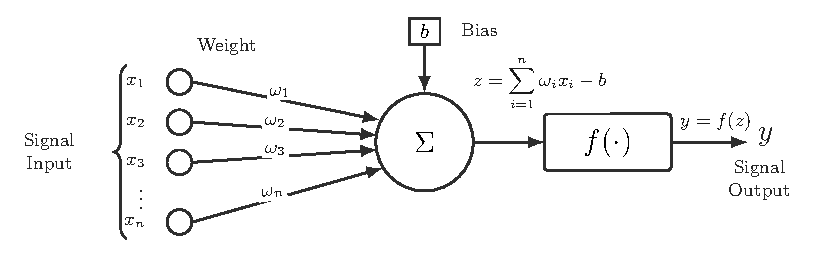
\includegraphics[width=0.82\textwidth]{neuron_perceptron_with_activation.pdf}
    \caption{A single artificial neuron with input vector $\vect{x}$, weight vector $\vect{w}$, bias $b$, and pre-activation output $z$. The activation function $f$ is applied to $z$ to produce the final output $y$.}
    \label{fig:neuron_affine_unit}
\end{figure}

The term $\vect{w}^T \vect{x}$ measures how strongly the input matches the learned weights. This affine computation is the basic operation repeated across layers in larger neural networks.

% !TEX root = ../../main_without_quantization.tex
\subsection{Activation Functions}

The neural network's ability to model complex patterns depends on the non-linear activation functions applied after each affine transformation. If we were to stack multiple layers without any non-linearity, the entire network would collapse into a single affine transformation.

Therefore, depth alone is not enough: neural networks require non-linear \textbf{activation functions} to model complex patterns \cite{Goodfellow2016}.

As shown in Figure~\ref{fig:neuron_affine_unit}, the activation function $f$ takes the pre-activation output $z$ and produces the final output $y=f(z)$. The choice of activation function can significantly affect the network's performance, convergence, and ability to learn from data.
\subsubsection{Classical Saturating Activations}

Sigmoid (Eq.\eqref{eq:sigmoid}) and hyperbolic tangent (Eq.\eqref{eq:tanh}) functions were often used in early networks. While these functions take real-valued inputs and output bounded values, which could be useful in the case of probabilities or normalized hidden states, they have very small derivatives when the input is very large or very small. This saturation causes learning to be very slow in deep networks \cite{Glorot2010,Goodfellow2016}.

\begin{equation}
    \label{eq:sigmoid}
    \sigma(x)=\frac{1}{1+e^{-x}}, \qquad \sigma:\mathbb{R}\rightarrow(0,1).
\end{equation}

\begin{equation}
    \label{eq:tanh}
    \tanh(x)=\frac{e^x-e^{-x}}{e^x+e^{-x}}, \qquad \tanh:\mathbb{R}\rightarrow(-1,1).
\end{equation}

\subsubsection{Rectified Activations}

Rectified Linear Units (ReLU) became common in deep learning because they are simple, computationally cheap, and reduce saturation for positive inputs \cite{Nair2010}. ReLU is defined as showing in Eq.\eqref{eq:relu}:
\begin{equation}
    \label{eq:relu}
    \operatorname{ReLU}(x)=\max(0,x), \qquad \operatorname{ReLU}:\mathbb{R}\rightarrow[0,\infty).
\end{equation}

Leaky ReLU keeps a small non-zero slope for negative inputs, reducing the risk that a unit becomes permanently inactive \cite{Maas2013}, as shown in Eq.\eqref{eq:leaky_relu}:
\begin{equation}
    \label{eq:leaky_relu}
    \operatorname{LeakyReLU}(x)=
    \begin{cases}
        x, & x \ge 0,\\
        \alpha x, & x<0,
    \end{cases}
    \qquad \alpha \in (0,1), \quad \operatorname{LeakyReLU}:\mathbb{R}\rightarrow\mathbb{R}.
\end{equation}

The Exponential Linear Unit (ELU) uses a smooth negative branch and a linear positive branch \cite{Clevert2016}, which can lead to faster convergence and improved performance in some cases, as shown in Eq.\eqref{eq:elu}:
\begin{equation}
    \label{eq:elu}
    \operatorname{ELU}(x)=
    \begin{cases}
        x, & x \ge 0,\\
        \alpha(e^x-1), & x<0,
    \end{cases}
    \qquad \alpha>0, \quad \operatorname{ELU}:\mathbb{R}\rightarrow(-\alpha,\infty).
\end{equation}

Modern Transformer architectures often use the Gaussian Error Linear Unit (GELU), a smooth activation that weights inputs by their value under the standard Gaussian cumulative distribution \cite{Hendrycks2016}, as shown in Eq.\eqref{eq:gelu}:
\begin{equation}
    \label{eq:gelu}
    \operatorname{GELU}(x)=x\Phi(x)\approx \frac{x}{2}\left(1+\tanh\left(\sqrt{\frac{2}{\pi}}(x+0.044715x^3)\right)\right).
\end{equation}

Figure~\ref{fig:activation_comparison} compares the shapes of these activation functions on the same input range. The plot makes the difference between saturating functions and rectified functions visible.

\begin{figure}[H]
    \centering
    \begin{tikzpicture}
        \begin{axis}[
            width=0.82\textwidth,
            height=6.2cm,
            xmin=-4, xmax=4,
            ymin=-1.4, ymax=4,
            axis lines=middle,
            xlabel={$x$},
            ylabel={$f(x)$},
            samples=200,
            grid=major,
            legend style={at={(0.02,0.98)},anchor=north west,font=\small},
        ]
            \addplot[deepmutedblue, very thick] {1/(1+exp(-x))};
            \addlegendentry{Sigmoid}
            \addplot[dustyteal, very thick] {tanh(x)};
            \addlegendentry{Tanh}
            \addplot[orange!85!black, very thick] {max(0,x)};
            \addlegendentry{ReLU}
            \addplot[slateblue, thick, dashed] {x < 0 ? 0.1*x : x};
            \addlegendentry{Leaky ReLU}
            \addplot[actreddark, thick, dashdotted] {x < 0 ? exp(x)-1 : x};
            \addlegendentry{ELU}
            \addplot[black, thick, dotted] {0.5*x*(1+tanh(sqrt(2/pi)*(x+0.044715*x^3)))};
            \addlegendentry{GELU}
        \end{axis}
    \end{tikzpicture}
    \caption{Comparison of common activation functions}
    \label{fig:activation_comparison}
\end{figure}

% !TEX root = ../../main_without_quantization.tex

\subsection{The Multi-Layer Perceptron (MLP)}

A single activated neuron can transform an input into a simple response, but practical models require many such units to work together. A Multi-Layer Perceptron extends the neuron model by organizing neurons into successive layers, so that each layer transforms the representation produced by the one before it.

Going from a single neuron to an MLP increases expressiveness by composing affine transformations with non-linear activations across layers~\cite{Rumelhart1986}. MLPs are \emph{feedforward} and typically \emph{fully connected}, meaning each neuron connects to all neurons in the next layer.

Eq.~\eqref{eq:mlp_layer_computation} formalizes the computation performed by each layer of an MLP, to transform the raw input $\vect{x}$ into the final output (prediction)$\vect{y}$.
\begin{equation}
\label{eq:mlp_layer_computation}
\begin{aligned}
	\vect{h}^{(0)} &= \vect{x},\\
	\vect{h}^{(\ell)} &= f(\matr{W}^{(\ell)}\vect{h}^{(\ell-1)} + \vect{b}^{(\ell)}) \quad \text{for } \ell = 1, 2, \ldots, L-1,\\
	\vect{y} &= f_{\text{out}}(\matr{W}^{(L)}\vect{h}^{(L-1)} + \vect{b}^{(L)}),
\end{aligned}
\end{equation}

	Figure~\ref{fig:mlp_architecture} illustrates a typical MLP with one input layer, two hidden layers, and one output layer.
\begin{figure}[ht]
    \centering
    \resizebox{0.82\textwidth}{!}{%
    \begin{tikzpicture}[
        scale=1.0,
        node distance=2.5cm,
        neuron/.style={circle, draw=black!70, fill=black!8, line width=1.4pt, minimum size=0.7cm},
        input/.style={circle, draw=black!85, fill=black!15, line width=1.6pt, minimum size=0.7cm},
        output/.style={circle, draw=black!70, fill=black!5, line width=1.4pt, minimum size=0.7cm},
        arrow/.style={-Stealth, color=black!30, thin},
        highlight/.style={-Stealth, color=black!65, very thick},
        annotation/.style={font=\scriptsize, color=black!65}
        ]

        % Input layer
        \foreach \i in {1,2,3,4} {
            \node[input] (x\i) at (0, -\i*1.2) {};   % was 1.5
        }
        \node[above=0.3cm of x1, color=black!75, font=\bfseries] {Input Layer};
        \node[right=0.2cm of x1, color=black!60, font=\small] {$x_1$};
        \node[right=0.2cm of x2, color=black!60, font=\small] {$x_2$};
        \node[right=0.2cm of x3, color=black!60, font=\small] {$x_3$};
        \node[right=0.2cm of x4, color=black!60, font=\small] {$x_4$};
        \node[below=0.3cm of x4, color=black!60, font=\small] {$\vect{h}^{(0)} \in \reals^{4}$};

        % Hidden layer 1
        \foreach \i in {1,2,3,4,5} {
            \node[neuron] (h1\i) at (4, -\i*1.1) {};   % was 1.3
        }
        \node[above=0.3cm of h11, color=black!75, font=\bfseries] {Hidden Layer 1};
        \node[below=0.3cm of h15, color=black!60, font=\small] {$\vect{h}^{(1)} \in \reals^{5}$};

        % Hidden layer 2
        \foreach \i in {1,2,3,4} {
            \node[neuron] (h2\i) at (8, -\i*1.2) {};   % was 1.5
        }
        \node[above=0.3cm of h21, color=black!75, font=\bfseries] {Hidden Layer 2};
        \node[below=0.3cm of h24, color=black!60, font=\small] {$\vect{h}^{(2)} \in \reals^{4}$};

        % Output layer
        \foreach \i in {1,2} {
            \node[output] (y\i) at (12, {-1.8-(\i-1)*1.8}) {};   % tightened gap
        }
        \node[above=0.3cm of y1, color=black!75, font=\bfseries] {Output Layer};
        \node[left=0.2cm of y1, color=black!60, font=\small] {$y_1$};
        \node[left=0.2cm of y2, color=black!60, font=\small] {$y_2$};
        \node[below=0.3cm of y2, color=black!60, font=\small] {$\vect{y} \in \reals^{2}$};

        % Connections: Input to Hidden 1
        \foreach \i in {1,2,3,4} {
            \foreach \j in {1,2,3,4,5} {
                \draw[arrow] (x\i) -- (h1\j);
            }
        }
        % Connections: Hidden 1 to Hidden 2
        \foreach \i in {1,2,3,4,5} {
            \foreach \j in {1,2,3,4} {
                \draw[arrow] (h1\i) -- (h2\j);
            }
        }
        % Connections: Hidden 2 to Output
        \foreach \i in {1,2,3,4} {
            \foreach \j in {1,2} {
                \draw[arrow] (h2\i) -- (y\j);
            }
        }

        % Highlight one example path
        \draw[highlight] (x2) -- (h13);
        \draw[highlight] (h13) -- (h22);
        \draw[highlight] (h22) -- (y1);

        % Weight matrix labels
        \node[color=black!65, font=\small\bfseries, align=center] at (2, -7.2) {$\matr{W}^{(1)}$\\[0.1cm] \scriptsize $(5 \times 4)$};
        \node[color=black!65, font=\small\bfseries, align=center] at (6, -7.2) {$\matr{W}^{(2)}$\\[0.1cm] \scriptsize $(4 \times 5)$};
        \node[color=black!65, font=\small\bfseries, align=center] at (10, -7.2) {$\matr{W}^{(3)}$\\[0.1cm] \scriptsize $(2 \times 4)$};

        % Bias vectors
        \node[annotation, align=center] at (2, -8.0) {$\vect{b}^{(1)} \in \reals^5$};
        \node[annotation, align=center] at (6, -8.0) {$\vect{b}^{(2)} \in \reals^4$};
        \node[annotation, align=center] at (10, -8.0) {$\vect{b}^{(3)} \in \reals^2$};

        % Activation annotations
        \node[annotation, align=center] at (2, 0.6) {$\vect{h}^{(1)} = \sigma(\matr{W}^{(1)}\vect{h}^{(0)} + \vect{b}^{(1)})$};
        \node[annotation, align=center] at (6, 0.6) {$\vect{h}^{(2)} = \sigma(\matr{W}^{(2)}\vect{h}^{(1)} + \vect{b}^{(2)})$};
        \node[annotation, align=center] at (10, 0.6) {$\vect{y} = \sigma(\matr{W}^{(3)}\vect{h}^{(2)} + \vect{b}^{(3)})$};

        % Legend
        \node[draw=black!30, fill=white, rounded corners, align=left, font=\scriptsize] at (15, -3) {
            \textbf{Legend:}\\[0.2cm]
            \tikz\draw[arrow] (0,0) -- (0.4,0); Weighted connection\\[0.15cm]
            \tikz\draw[highlight] (0,0) -- (0.4,0); Example path\\[0.15cm]
            \tikz\node[input, minimum size=0.4cm] at (0.2,0) {}; Input neuron\\[0.15cm]
            \tikz\node[neuron, minimum size=0.4cm] at (0.2,0) {}; Hidden neuron\\[0.15cm]
            \tikz\node[output, minimum size=0.4cm] at (0.2,0) {}; Output neuron
        };

        % Parameter count box
        \node[draw=black!30, fill=black!5, rounded corners, align=center, font=\scriptsize] at (6, -9.0) {
            \textbf{Total Parameters:} $(5\times4) + 5 + (4\times5) + 4 + (2\times4) + 2 = 59$
        };

        % Top annotation
        \node[annotation, font=\small\bfseries] at (6, 1.4) {Layer-wise composition of affine maps and activations};

    \end{tikzpicture}
    }
    \caption{Fully connected MLP with 4 input features, two hidden layers (5 and 4 neurons), and 2 output neurons.}
    \label{fig:mlp_architecture}
\end{figure}
\newpage
%The diagram shows the layer-wise transformations that define an MLP. The input layer stores the feature vector $\vect{h}^{(0)}=\vect{x}$. The first hidden layer computes $\vect{h}^{(1)}$ from all input features using $\matr{W}^{(1)}$ and $\vect{b}^{(1)}$, then applies a non-linearity. The second hidden layer repeats the same operation on $\vect{h}^{(1)}$, producing $\vect{h}^{(2)}$. Finally, the output layer maps the last hidden representation to the prediction vector $\vect{y}$. The highlighted orange path illustrates one route by which information from a single input feature can influence an output neuron, and the pale connections show that every layer is fully connected to the next.

%\subsection{Hidden Representations}
%
%The hidden layers of an MLP are its internal states. The $i$-th hidden layer effectively performs the $i$-th transformation of the data, mapping it into the $i$-th coordinate space discovered through training. The earlier hidden layers perform combinations of input features, while the later layers perform combinations of the earlier layer outputs, creating higher-level representations related to the task in question. The output of the last hidden layer is typically transformed into the appropriate output space. For classification, this means class scores or probabilities. For regression, it means one or more continuous values.
%
%The multi-layer representation is helpful, but it suffers from an obvious limitation. The MLP accepts its input as a single vector; therefore, there is no innate reason in the model for elements close to each other to be related, or for the elements of the vector to have an order. If such structure is required, it must be supplied by the architecture, which we will tackle later in Section~\ref{sec:specialized_architectures}.
%
%For now, we remain with the MLP and ask a more basic question.
%Once the architecture has fixed how information can flow from inputs to outputs, how are the actual parameters of this flow chosen? This is the role of learning: the weights and biases must be adjusted from data so that the network output becomes closer to the desired target. The next section \ref{sec:Optimization and Gradients}
%formulates this process as an optimization problem.

% !TEX root = ../../main_without_quantization.tex
\section{Optimization and Gradients}\label{sec:Optimization and Gradients}

We outlined how an MLP generates a prediction: by a composition of transformations applied at each layer. With forward computation, learning can be thought of as figuring out what the weights and biases should be given the data. Network construction then becomes an optimization problem: select the parameters that make the output as close as possible to the target on a training set.

Hence, a quantitative measure must be provided that can actually be minimized; this provides the rationale for empirical risk minimization.

\subsection{Empirical Risk Minimization}

Given a dataset $\mathcal{D} = \{(\vect{x}^{(i)}, y^{(i)})\}_{i=1}^{m}$, learning consists of finding parameters $\params$ that minimize the discrepancy between the model predictions $f_{\params}(\vect{x})$ and the target values. This is commonly formulated as empirical risk minimization \cite{Vapnik1998}:
\begin{equation}
    \params^* = \arg\min_{\params} \hat{R}(\params) = \arg\min_{\params} \frac{1}{m} \sum_{i=1}^{m} \loss(f_{\params}(\vect{x}^{(i)}), y^{(i)}).
    \label{eq:erm}
\end{equation}
where $m$ is the number of training samples; $\vect{x}^{(i)}$ and $y^{(i)}$ are the input and target of the $i$-th sample; $\params$ are the model parameters; $\hat{R}(\params)$ is the empirical risk, i.e.\ the average loss over the training set; and $\loss(\cdot,\cdot)$ is the per-sample loss function. For a $K$-class classification problem the prediction is a probability vector $\hat{\vect{y}} \in \Delta^{K}$ (the probability simplex over $K$ classes) with entries $\hat{y}_k$, the target $\vect{y}$ has entries $y_k$, and $c$ denotes the index of the true class; the Kullback--Leibler divergence ~\cite{cover2006}
$D_{\text{KL}}(\vect{y} \,\|\, \hat{\vect{y}})$ measures the excess cost of using $\hat{\vect{y}}$ in place of $\vect{y}$.

This empirical-risk objective in Eq.~\eqref{eq:erm} gives the general learning template: choose parameters by minimizing the average loss over the training set. It does not specify the loss itself. That choice is determined by the problem and the structure of the output.

\subsubsection{Loss Functions}

Now we have an optimization problem. But what are we minimizing? A loss function accounts for the discrepancy between predictions and targets and makes explicit assumptions about the problem and the output space. Table~\ref{tab:loss_functions} summarizes the most common loss functions used in neural network training, along with their formulas, target types, and properties. The choice of loss function depends on the task at hand (classification vs regression) and the nature of the targets (hard one-hot labels, soft probability distributions, or continuous real values.).
%\subsubsection{Cross-Entropy Loss}
%
%For classification tasks, neural networks typically produce a probability distribution over $K$ classes via a softmax output. Given a predicted distribution $\hat{\vect{y}} \in \Delta^{K}$ and a target distribution $\vect{y}$ (often a one-hot vector), the cross-entropy loss is defined as:
%\begin{equation}
%    \loss_{\text{CE}}(\hat{\vect{y}}, \vect{y}) = -\sum_{k=1}^{K} y_k \log \hat{y}_k.
%    \label{eq:ce}
%\end{equation}
%The cross-entropy expression in Equation~\eqref{eq:ce} quantifies the number of bits required on average to encode symbols from $\vect{y}$ using a code optimal for $\hat{\vect{y}}$. For a hard one-hot label, this becomes the negative log-likelihood of the true class $\loss_{\text{CE}} = -\log \hat{y}_c$, where $c$ is the index of the true class. This has the effect of pushing most of the probability mass onto the correct class, and preventing it from going anywhere else. For a hard label, this works out fine, but the moment the target becomes a distribution instead of a single class, the problem becomes more explicitly about how to quantify distance between distributions, which motivates the following point.
%
%\subsubsection{Kullback--Leibler Divergence}
%
%Cross-entropy implicitly compares two distributions, which raises a natural question: what is the right way to measure how far apart two probability distributions are? The Kullback--Leibler (KL) divergence \cite{Kullback1951} provides a principled answer rooted in information theory. Rather than measuring total encoding cost, it isolates the \emph{excess} cost incurred by using $\hat{\vect{y}}$ in place of the true distribution $\vect{y}$:
%\begin{equation}
%    D_{\text{KL}}(\vect{y} \,\|\, \hat{\vect{y}}) = \sum_{k=1}^{K} y_k \log \frac{y_k}{\hat{y}_k}.
%    \label{eq:kl}
%\end{equation}
%Expanding the KL divergence in Equation~\eqref{eq:kl} reveals the exact relationship with cross-entropy:
%\begin{equation}
%    D_{\text{KL}}(\vect{y} \,\|\, \hat{\vect{y}})
%    = \underbrace{-\sum_{k} y_k \log \hat{y}_k}_{\loss_{\text{CE}}(\hat{\vect{y}},\,\vect{y})}
%    \;-\; \underbrace{\left(-\sum_{k} y_k \log y_k\right)}_{H(\vect{y})},
%    \label{eq:kl_ce_decomp}
%\end{equation}
%where $H(\vect{y})$ is the entropy of the target distribution. The decomposition in Equation~\eqref{eq:kl_ce_decomp} shows why cross-entropy and KL divergence lead to the same optimization problem when the target distribution is fixed: $H(\vect{y})$ does not depend on the model parameters. If the target is a one-hot label then $H(\vect{y}) = 0$ and the two functions are equal; if the target is a soft distribution, then $H(\vect{y}) > 0$, and KL divergence is the clearly superior objective. The above loss functions are for when the output is a discrete probability distribution. For real-valued regression problems, an alternative family of loss functions are used.
%
%\subsubsection{Regression Losses}
%
%For regression, the output is a continuous value rather than a class index, and the appropriate loss changes accordingly. The mean squared error (MSE) is the standard choice:
%\begin{equation}
%    \loss_{\text{MSE}}(\hat{y}, y) = \frac{1}{m}\sum_{i=1}^{m}(\hat{y}^{(i)} - y^{(i)})^2.
%    \label{eq:mse}
%\end{equation}
%The MSE objective in Equation~\eqref{eq:mse} penalizes large regression errors quadratically. Under a Gaussian noise assumption on the targets, minimizing it is equivalent to maximum likelihood estimation of the model parameters. When the output distribution is heavier-tailed or contains outliers, the mean absolute error (L1 loss) $\loss_{\text{MAE}} = \frac{1}{m}\sum_i |\hat{y}^{(i)} - y^{(i)}|$ is more robust, as it does not square large deviations.
%
%\noindent\rule{0.4\linewidth}{0.55pt}
\begin{table}[ht]
\centering
\caption{Summary of common neural network loss functions.}
\label{tab:loss_functions}
\renewcommand{\arraystretch}{1.45}
\begin{tabularx}{\textwidth}{@{} l l X l X @{}}
\toprule
\textbf{Loss} & \textbf{Task} & \textbf{Formula} & \textbf{Target type} & \textbf{properties} \\
\midrule

Cross-Entropy
  & Classification
  & $\loss_{\text{CE}}(\hat{\vect{y}}, \vect{y}) = -\displaystyle\sum_{k=1}^{K} y_k \log \hat{y}_k$
  & Soft or one-hot
  & Measures total encoding cost of $\vect{y}$ under code optimal for $\hat{\vect{y}}$;
    reduces to $-\log\hat{y}_c$ for hard labels. \\

KL Divergence
  & Classification
  & $D_{\text{KL}}(\vect{y}\,\|\,\hat{\vect{y}}) = \displaystyle\sum_{k=1}^{K} y_k \log \dfrac{y_k}{\hat{y}_k}$
  & Soft distribution
  & Measures \emph{excess} encoding cost;
    $D_{\text{KL}} = \loss_{\text{CE}} - H(\vect{y})$.
    Preferred over CE when targets are soft. \\

MSE (L2)
  & Regression
  & $\loss_{\text{MSE}}(\hat{y}, y) = \dfrac{1}{m}\displaystyle\sum_{i=1}^{m}(\hat{y}^{(i)} - y^{(i)})^2$
  & Continuous
  & Penalises errors quadratically; equivalent to maximum likelihood estimation (MLE) under Gaussian noise.
    Sensitive to outliers. \\

MAE (L1)
  & Regression
  & $\loss_{\text{MAE}}(\hat{y}, y) = \dfrac{1}{m}\displaystyle\sum_{i=1}^{m}|\hat{y}^{(i)} - y^{(i)}|$
  & Continuous
  & Penalises errors linearly; robust to heavy-tailed distributions and outliers. \\

\bottomrule
\end{tabularx}

\smallskip
\begin{tabularx}{\textwidth}{@{} X @{}}
\small
\textbf{Notes.}
$K$: number of classes;
$\hat{\vect{y}}\in\Delta^{K}$: predicted probability vector (softmax output);
$\vect{y}$: target distribution (one-hot or soft);
$c$: index of the true class;
$H(\vect{y}) = -\sum_k y_k\log y_k$: entropy of the target;
$m$: number of samples;
$\hat{y}^{(i)}, y^{(i)}$: predicted and true scalar outputs for sample $i$.
When $\vect{y}$ is one-hot, $H(\vect{y})=0$ and $D_{\text{KL}}=\loss_{\text{CE}}$.
\\
\end{tabularx}
\end{table}

% !TEX root = ../../main_without_quantization.tex
\subsection{Algorithms for Gradient-Based Optimization}
\label{sec:gradient_based_optimization}
With the loss function established, the remaining question is how the resulting error signal propagates back through the network to update the parameters.

Training neural networks is usually a problem of finding a parameter vector $\theta \in \mathbb{R}^{d}$ that minimizes the scalar objective $J(\theta)$ where $J$ is the empirical risk defined by the loss function and the training data. Formally, we want to solve \eqref{eq:optimization_problem}:
\begin{equation}
    \theta^* = \arg\min_{\theta} J(\theta).
    \label{eq:optimization_problem}
\end{equation}

The parameter space in most contemporary neural networks is high-dimensional and the objective is largely non-convex so a solution in closed form for optimum parameters rarely exists. Training is hence iterative: the parameters are updated according to directions suggested by the gradient of the loss \cite{Bottou2018}.

The gradient $\nabla J(\theta)$ indicates the direction of steepest local increase of the objective, and optimizers will use it in reverse to adjust the parameters to  yield a lower loss. This concept forms the basis of the gradient descent algorithm as well as of all the adaptive optimization schemes currently used in training neural networks.

\subsubsection{Gradient Descent}

Gradient descent updates parameters in the negative-gradient direction. For iteration $t$ and learning rate $\eta>0$, the update is formulated in Eq.\eqref{eq:gradient_descent}:
\begin{equation}
    \label{eq:gradient_descent}
    \theta_{t+1} = \theta_t - \eta \nabla J(\theta_t).
\end{equation}

The learning rate controls the step size. If it is too small, optimization may progress slowly; if it is too large, the updates can overshoot useful regions of the objective surface. In large scale learning, the exact gradient over the full dataset is often replaced by a stochastic estimate computed on a mini-batch. This gives stochastic gradient descent, which is cheaper per update and is widely used for neural-network training \cite{Bottou2018}.

\subsubsection{Adam}

Adam is an adaptive gradient-based optimizer that combines momentum with per-parameter learning-rate adaptation \cite{kingma2015}. Instead of using only the current gradient, Adam keeps exponential moving averages of the first and second moments of the gradient, which are updated as shown in Eq.\eqref{eq:adam_moments}:
\begin {equation}
    \label{eq:adam_moments}
    m_t = \beta_1 m_{t-1} + (1-\beta_1)g_t,
    \qquad
    v_t = \beta_2 v_{t-1} + (1-\beta_2)g_t^2,
\end{equation}

%\begin{align}
%    m_t &= \beta_1 m_{t-1} + (1-\beta_1)g_t,\\
%    v_t &= \beta_2 v_{t-1} + (1-\beta_2)g_t^2,
%\end{align}
where $g_t=\nabla J(\theta_t)$ is the gradient estimate at iteration $t$, $m_t$ tracks the average direction of recent gradients, and $v_t$ tracks their squared magnitude.

Because both moving averages are initialized at zero, Adam applies bias correction computed as follows Eq.\eqref{eq:adam_bias_correction}:
\begin{equation}
    \label{eq:adam_bias_correction}
    \hat{m}_t = \frac{m_t}{1-\beta_1^t},
    \qquad
    \hat{v}_t = \frac{v_t}{1-\beta_2^t}.
\end{equation}
The parameter update is then given by \eqref{eq:adam_update}:
\begin{equation}
    \label{eq:adam_update}
    \theta_{t+1}
    =
    \theta_t
    -
    \eta \frac{\hat{m}_t}{\sqrt{\hat{v}_t}+\epsilon}.
\end{equation}

Adam is often utilized due to its robustness in relation to scaling differences among gradients for different parameters and typically requires less fine-tuning of learning rates as opposed to simple gradient descent. Subsequent versions of Adam include AdamW, which removes the weight decay from the adaptive learning component and is applicable to a variety of deep learning applications \cite{Loshchilov2019}.



Both gradient descent and Adam describe how the parameters should be updated, but they both require that the gradients be available. These computations can become expensive in deep, multi-layered networks and thus require an alternative method, termed backpropagation.
\subsection{Backpropagation}

Backpropagation computes these gradients efficiently by applying the chain rule from the output layer back through the network \cite{Rumelhart1986}. In compact form, it provides the quantities
$\nabla_{\theta}\mathcal{L}$
where $\theta$ denotes the trainable parameters and $\mathcal{L}$ is the loss function.

In the case of this pruning-oriented report we do not require the full derivation above. It is sufficient that back-propagation relates model error to specific parameters and structures, which will be exploited by the gradient-based pruning criteria, Taylor approximation, Fisher scores and post-pruning recovery process detailed in later chapters.

\section{Conclusion}

In this chapter, we have established the mathematical and optimization framework of deep neural networks. We described the building blocks-the affine and non-linear transformation of feed forward networks and formulated training of a feed forward network as an empirical risk minimization problem. We also described the central optimization concepts of gradient and Hessian matrices, crucial to the learning process of the networks and to pruning algorithms in assessing parameters relevance.


Though the above theory applies to any feed-forward network, the architecture used in modern NLP are often extremely specialized. To know how pruning is practically applied one must be aware of the mapping of generic matrix operations to the structures within an architecture. Therefore the subsequent chapter deals solely with the Transformer architecture and its components, how parameters are structured and the drastic bottleneck which necessitates compression.
\chapter{Transformer Architectures and Efficiency}
\label{sec:specialized_architectures}

\section{Introduction}
While Multi-Layer Perceptrons offer a generic learning model over vector inputs, they do not inherently leverage any underlying structure of the data. For this report, the architecture of interest is the Transformer. Since its introduction, the Transformer’s ability to model long-range dependencies in parallel has made it the foundation of state-of-the-art sequence modeling. However, this expressive power comes at a severe computational cost. To effectively compress such a model, one cannot treat it as a generic sequence of matrices; rather, one must deeply understand its internal wiring, where its parameters are concentrated, and how data moves through its layers during execution.

The purpose of this chapter is to dissect the Transformer architecture specifically through the lens of computational cost and structural parameterization. The chapter begins by detailing the core building blocks of the network—namely, the Multi-Head Attention mechanism and the position-wise Feed-Forward Networks (FFNs). Special emphasis is placed on the matrix dimensions and structural design of these components, as they dictate the exact locations of the parameters that pruning algorithms will later target.

Building on these components, the chapter then examines the complete Encoder-Decoder architecture before shifting focus to the primary motivation for this report: the computational bottleneck. We analyze the quadratic scaling of self-attention and the massive memory footprints of dense weight matrices. Finally, the chapter introduces hardware-aware efficiency metrics, such as FLOPs, memory bandwidth, and latency.



%, which has become the dominant model for sequence modeling tasks, particularly in natural language processing, and is the target of the compression methods discussed in later chapters.

%\subsection{Convolutional Neural Networks (CNNs)}
%
%CNNs are feedforward networks optimized for grid-like data, such as images. They stack multiple modules, typically consisting of:
%
%\begin{figure}[htbp]
%    \centering
%    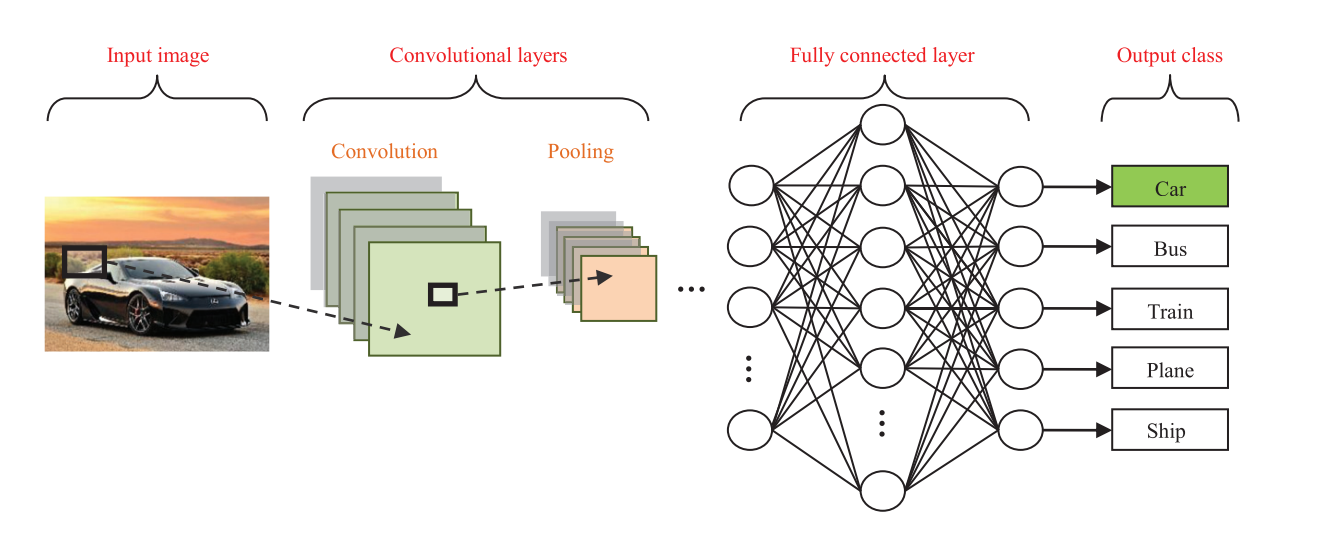
\includegraphics[width=0.85\textwidth]{figures/foundations/cnn_classification_pipeline}
%    \caption{Simple CNN architecture: input, convolution + activation, pooling, and fully connected layers \cite{Waseem2017}.}
%    \label{fig:cnn-simple}
%\end{figure}
%
%\begin{itemize}
%    \item \textbf{Convolutional Layers:} These act as feature extractors. A learnable filter (kernel) $K$ slides over the input $I$, performing element-wise multiplication and summation to create a feature map $S$. The operation is defined as:
%    \[
%    S(i, j) = (I * K)(i, j) = \sum_{m} \sum_{n} I(i+m, j+n) K(m, n)
%    \]
%    \item \textbf{Pooling Layers:} These reduce the spatial dimensions (width and height) of feature maps using summary statistics (e.g., Max or Average pooling) to decrease computational cost and overfitting.
%\end{itemize}
%
%\subsection{Recurrent Neural Networks (RNNs)}
%RNNs are designed for sequential data (e.g., time series, text). Unlike feedforward networks, RNNs utilize cyclic connections to maintain a \textit{hidden state} that captures historical information. The network dynamics are described by:
%\[
%h_t = \sigma(W_{hh} h_{t-1} + W_{xh} x_t + b_h)
%\]
%\[
%y_t = W_{hy} h_t + b_y
%\]
%where \( h_t \) is the hidden state, \( x_t \) the input, and \( y_t \) the output at time \( t \).
%\begin{figure}[htbp]
%  \centering
%  \begin{tikzpicture}[>=Stealth, node distance=10mm and 18mm, every node/.style={font=\small}]
%    \tikzstyle{inp} = [circle, draw=slateblue, fill=mistyblue!20, minimum size=7mm]
%    \tikzstyle{hid} = [rectangle, draw=dustyteal, fill=sagegreen!20, minimum size=9mm]
%    \tikzstyle{outnode} = [circle, draw=slateblue, fill=mistyblue!20, minimum size=7mm]
%    \tikzstyle{lbl} = [font=\scriptsize, color=slateblue]
%
%    % Inputs (bottom layer)
%    \node[inp] (x1) {$x_1$};
%    \node[inp] (x2) [right=of x1] {$x_2$};
%    \node[inp] (x3) [right=of x2] {$x_3$};
%    \node (xd) [right=of x3] {$\dots$};
%    \node[inp] (xT) [right=of xd] {$x_T$};
%
%    % Hidden (middle layer)
%    \node[hid] (h1) [above=of x1] {$h_1$};
%    \node[hid] (h2) [above=of x2] {$h_2$};
%    \node[hid] (h3) [above=of x3] {$h_3$};
%    \node[hid] (hT) [above=of xT] {$h_T$};
%    \node (hd) [right=of h3] {$\dots$};
%
%    % Outputs (top layer)
%    \node[outnode] (y1) [above=of h1] {$y_1$};
%    \node[outnode] (y2) [above=of h2] {$y_2$};
%    \node[outnode] (y3) [above=of h3] {$y_3$};
%    \node[outnode] (yT) [above=of hT] {$y_T$};
%
%    % Input to hidden
%    \draw[->] (x1) -- node[midway, left, lbl] {$W_{xh}$} (h1);
%    \draw[->] (x2) -- node[midway, left, lbl] {$W_{xh}$} (h2);
%    \draw[->] (x3) -- node[midway, left, lbl] {$W_{xh}$} (h3);
%    \draw[->] (xT) -- node[midway, left, lbl] {$W_{xh}$} (hT);
%
%    % Hidden recurrence
%    \draw[->] (h1) to[bend left=8] node[midway, above, lbl] {$W_{hh}$} (h2);
%    \draw[->] (h2) to[bend left=8] node[midway, above, lbl] {$W_{hh}$} (h3);
%    \draw[->] (h3) -- (hd);
%    \draw[->] (hd) to[bend left=8] node[midway, above, lbl] {$W_{hh}$} (hT);
%
%    % Hidden to Output
%    \draw[->] (h1) -- node[midway, left, lbl] {$W_{hy}$} (y1);
%    \draw[->] (h2) -- node[midway, left, lbl] {$W_{hy}$} (y2);
%    \draw[->] (h3) -- node[midway, left, lbl] {$W_{hy}$} (y3);
%    \draw[->] (hT) -- node[midway, left, lbl] {$W_{hy}$} (yT);
%
%    \node[below left=2mm and 6mm of h1, font=\scriptsize] (h0label) {$h_0$};
%    \draw[->] (h0label.north) to[bend left=20] (h1.west);
%  \end{tikzpicture}
%  \caption{RNN unrolled in time.}
%  \label{fig:rnn-compact}
%\end{figure}
%
%\subsection{Autoencoders (AEs)}
%
%Autoencoders are neural networks designed for unsupervised learning of efficient data codings. They act as an identity function that learns to compress and then reconstruct data. An AE consists of two main parts:
%
%\begin{figure}[htbp]
%    \centering
%    \begin{tikzpicture}[>=Stealth, node distance=15mm, every node/.style={font=\small}]
%
%        % Define styles matching your previous RNN colors
%        % If these colors are defined in your preamble, you can remove these \definecolor lines
%        \definecolor{slateblue}{RGB}{106,90,205}
%        \definecolor{mistyblue}{RGB}{224,238,238}
%        \definecolor{dustyteal}{RGB}{76,146,147}
%        \definecolor{sagegreen}{RGB}{193,225,193}
%
%        \tikzstyle{neuron} = [circle, draw=slateblue, fill=mistyblue!20, minimum size=7mm, inner sep=0pt]
%        \tikzstyle{bottleneck} = [circle, draw=dustyteal, fill=sagegreen!20, minimum size=7mm, inner sep=0pt]
%        \tikzstyle{lbl} = [font=\scriptsize, color=slateblue]
%
%        % --- Nodes ---
%
%        % Input Layer (x)
%        \node[neuron] (i1) at (0, 2.0) {};
%        \node[neuron] (i2) at (0, 1.0) {};
%        \node[neuron] (i3) at (0, 0.0) {};
%        \node[neuron] (i4) at (0, -1.0) {};
%        \node[neuron] (i5) at (0, -2.0) {};
%
%        % Encoder Hidden
%        \node[neuron] (e1) at (2, 1.2) {};
%        \node[neuron] (e2) at (2, 0) {};
%        \node[neuron] (e3) at (2, -1.2) {};
%
%        % Bottleneck / Latent Space (z)
%        \node[bottleneck] (z1) at (4, 0.5) {};
%        \node[bottleneck] (z2) at (4, -0.5) {};
%
%        % Decoder Hidden
%        \node[neuron] (d1) at (6, 1.2) {};
%        \node[neuron] (d2) at (6, 0) {};
%        \node[neuron] (d3) at (6, -1.2) {};
%
%        % Output Layer (x_hat)
%        \node[neuron] (o1) at (8, 2.0) {};
%        \node[neuron] (o2) at (8, 1.0) {};
%        \node[neuron] (o3) at (8, 0.0) {};
%        \node[neuron] (o4) at (8, -1.0) {};
%        \node[neuron] (o5) at (8, -2.0) {};
%
%        % --- Connections ---
%
%        % Input -> Encoder
%        \foreach \i in {1,...,5}
%            \foreach \j in {1,...,3}
%                \draw[->, slateblue!40] (i\i) -- (e\j);
%
%        % Encoder -> Bottleneck
%        \foreach \i in {1,...,3}
%            \foreach \j in {1,...,2}
%                \draw[->, slateblue!40] (e\i) -- (z\j);
%
%        % Bottleneck -> Decoder
%        \foreach \i in {1,...,2}
%            \foreach \j in {1,...,3}
%                \draw[->, slateblue!40] (z\i) -- (d\j);
%
%        % Decoder -> Output
%        \foreach \i in {1,...,3}
%            \foreach \j in {1,...,5}
%                \draw[->, slateblue!40] (d\i) -- (o\j);
%
%        % --- Labels ---
%
%        \node[below=0.2cm of i5] {Input $x$};
%        \node[below=0.2cm of o5] {Output $\hat{x}$};
%        \node[below=0.2cm of z2, align=center] {Latent\\Space $z$};
%
%        % Braces for Encoder/Decoder
%        \draw[decorate, decoration={brace, amplitude=10pt, raise=5pt}, thick, slateblue] (i1.north) -- (z1.north) node[midway, above=20pt] {\textbf{Encoder}};
%        \draw[decorate, decoration={brace, amplitude=10pt, raise=5pt}, thick, slateblue] (z1.north) -- (o1.north) node[midway, above=20pt] {\textbf{Decoder}};
%
%    \end{tikzpicture}
%    \caption{Autoencoder architecture: The input is compressed into a lower-dimensional latent space (Bottleneck) and then reconstructed.}
%    \label{fig:autoencoder}
%\end{figure}
%
%\begin{itemize}
%    \item \textbf{Encoder:} Maps the high-dimensional input $x$ to a lower-dimensional latent representation $z$.
%    \item \textbf{Decoder:} Reconstructs the output $\hat{x}$ from the latent representation $z$.
%\end{itemize}
%
%The network is trained to minimize the reconstruction error (e.g., Mean Squared Error) between the input and the output:
%\[
%L(x, \hat{x}) = || x - \hat{x} ||^2
%\]
%By forcing data through a bottleneck, the network learns to capture the most salient features of the data distribution.
%

\newpage
\section{Transformer Networks}

Transformer networks, introduced by \cite{vaswani2017attention}, changed sequence modeling by replacing recurrent processing with attention-based computation. Instead of processing tokens one after another, a Transformer can compare tokens across the whole sequence in parallel. This makes it highly effective for language modelling, translation, summarization, and other sequence tasks. The original architecture was an encoder-decoder model for machine translation, while later systems often use encoder-only variants such as BERT \cite{devlin2019bert} or decoder-only variants such as LLaMA \cite{touvron2023llama2}.

\section{Core Architectural Components: Building Blocks of the Transformer}

Before separating the model into encoder and decoder stacks, it is useful to define the components repeated inside those stacks. Transformer layers are built from token embeddings, positional information, attention projections, feed-forward channels, residual connections, and normalization layers. These components are also the main targets for compression, because they determine both parameter count and runtime cost.

\subsubsection{Input Representation: Embeddings and Positional Encoding}

Every token is mapped to a continuous embedding vector. Since self-attention does not inherently encode token order, positional information is added to the token representations. The original Transformer uses sinusoidal positional encodings \cite{vaswani2017attention}, shown in Eq.\eqref{eq:positional_encoding}, where $d_{\text{model}}$ is the embedding dimension and $i$ indexes the dimensions of the positional encoding:
\begin{equation}
  \label{eq:positional_encoding}
    PE_{(\text{pos}, 2i)} = \sin\left(\frac{\text{pos}}{10000^{2i/d_{\text{model}}}}\right), \quad
    PE_{(\text{pos}, 2i+1)} = \cos\left(\frac{\text{pos}}{10000^{2i/d_{\text{model}}}}\right).
\end{equation}

\subsubsection{Self-Attention Mechanism}

Self-attention allows each token representation to aggregate information from the rest of the sequence. The mechanism uses three learned projections of each input: queries, keys, and values \cite{vaswani2017attention}. Queries represent what a token is looking for, keys represent what each token offers for comparison, and values contain the information that will be aggregated.

For an input sequence representation $\matr{X} \in \reals^{n \times d_{\text{model}}}$, the projections are computed as shown in Eq.\eqref{eq:attention_projections}, where $\matr{W}^{Q}, \matr{W}^{K}, \matr{W}^{V} \in \reals^{d_{\text{model}} \times d_k}$ are learned weight matrices for queries, keys, and values respectively:
\begin{equation}
  \label{eq:attention_projections}
    \matr{Q} = \matr{X}\matr{W}^{Q}, \quad
    \matr{K} = \matr{X}\matr{W}^{K}, \quad
    \matr{V} = \matr{X}\matr{W}^{V}.
\end{equation}

Scaled dot-product attention is then computed as shown in Eq.\eqref{eq:scaled_dot_product_attention}, where $d_k$ is the dimension of the queries and keys:
\begin{equation}
  \label{eq:scaled_dot_product_attention}
    \operatorname{Attention}(\matr{Q}, \matr{K}, \matr{V})
    =
    \operatorname{softmax}\left(\frac{\matr{Q}\matr{K}^{\top}}{\sqrt{d_k}}\right)\matr{V}.
\end{equation}
The factor $\sqrt{d_k}$ prevents dot products from becoming too large, which would push the softmax into saturated regions with weak gradients.

\subsubsection{Multi-Head Attention}

Multi-head attention applies several attention mechanisms in parallel, allowing the model to attend to different representation subspaces and token relationships at the same time \cite{vaswani2017attention}. Eq.\eqref{eq:multi_head_attention} defines the computation for each head $i$, where $\matr{W}^{Q}_{i}, \matr{W}^{K}_{i}, \matr{W}^{V}_{i} \in \reals^{d_{\text{model}} \times d_k}$ are the projection matrices for head $i$:
\begin{equation}
  \label{eq:multi_head_attention}
    \operatorname{head}_i =
    \operatorname{Attention}(\matr{X}\matr{W}^{Q}_{i}, \matr{X}\matr{W}^{K}_{i}, \matr{X}\matr{W}^{V}_{i}),
    \quad i = 1,\ldots,h.
\end{equation}

The head outputs are concatenated and projected back to the model dimension as expressed in Eq.\eqref{eq:multi_head_concat_projection}, where $\matr{W}^{O} \in \reals^{hd_v \times d_{\text{model}}}$ is the output projection matrix:
\begin{equation}
  \label{eq:multi_head_concat_projection}
    \operatorname{MultiHead}(\matr{X}) =
    \operatorname{Concat}(\operatorname{head}_1,\ldots,\operatorname{head}_h)\matr{W}^{O}.
\end{equation}
\subsubsection{Feed-Forward Network}

After attention mixes information across tokens, a position-wise Feed-Forward Network (FFN) processes each token representation independently
The FFN usually expands the hidden representation to a larger intermediate dimension $d_{ff}$ and then projects it back to $d_{\text{model}}$. In the original Transformer, $d_{ff}$ is typically much larger than $d_{\text{model}}$, making FFN channels a major source of parameters and a natural target for structured pruning.

\subsubsection{Residual Connections and Layer Normalization}

Each attention or FFN sub-layer is wrapped by a residual path and layer normalization. Residual connections preserve a direct path for information and gradients, while normalization stabilizes the scale of hidden representations. This design is essential for training deep Transformer stacks and is also important when later compression methods remove heads, channels, or blocks \cite{vaswani2017attention,He2016,Ba2016}.

\subsection{Encoder and Decoder Architecture}

With the core components defined, the encoder and decoder can be described cleanly. The full encoder-decoder Transformer contains two main stacks:
\begin{itemize}
    \item \textbf{Encoder:} Processes the complete input sequence in parallel and produces contextual source representations.
    \item \textbf{Decoder:} Generates the output sequence autoregressively while attending to both previous target tokens and the encoder output.
\end{itemize}

The encoder converts the source sequence into a contextual memory representation $\matr{H}_{\text{enc}}$. The decoder uses this memory through cross-attention while also using masked self-attention to prevent access to future target tokens. The complete architecture is shown in Figure~\ref{fig:transformer-architecture}.

\begin{figure}[H]
  \centering
  \begin{tikzpicture}[scale=1.2, transform shape]
    \tikzstyle{Sanode} = [minimum height=1.4em, minimum width=7em, inner sep=3pt, rounded corners=1.5pt, draw=slateblue, fill=mistyblue!30]
    \tikzstyle{Resnode} = [minimum height=1.1em, minimum width=7em, inner sep=3pt, rounded corners=1.5pt, draw=dustyteal, fill=softgray!30]
    \tikzstyle{ffnnode} = [minimum height=1.4em, minimum width=7em, inner sep=3pt, rounded corners=1.5pt, draw=slateblue, fill=sagegreen!30]
    \tikzstyle{outputnode} = [minimum height=1.4em, minimum width=7em, inner sep=3pt, rounded corners=1.5pt, draw=slateblue, fill=mistyblue!50]
    \tikzstyle{inputnode} = [minimum height=1.4em, minimum width=3.5em, inner sep=3pt, rounded corners=1.5pt, draw=dustyteal, fill=mistyblue!20]
    \tikzstyle{posnode} = [minimum height=1.4em, minimum width=3.5em, inner sep=3pt, rounded corners=1.5pt, draw=dustyteal, fill=softgray!50]
    \tikzstyle{standard} = [rounded corners=3pt]

    \node [Sanode, anchor=west] (sa1) at (0,0) {\tiny \textbf{Self-Attention}};
    \node [Resnode, anchor=south] (res1) at ([yshift=0.3em]sa1.north) {\tiny \textbf{Add \& LayerNorm}};
    \node [ffnnode, anchor=south] (ffn1) at ([yshift=1em]res1.north) {\tiny \textbf{FFN}};
    \node [Resnode, anchor=south] (res2) at ([yshift=0.3em]ffn1.north) {\tiny \textbf{Add \& LayerNorm}};
    \node [inputnode, anchor=north west] (input1) at ([yshift=-1em,xshift=-0.5em]sa1.south west) {\tiny \textbf{Emb.}};
    \node [] (add1) at ([yshift=-1.6em,xshift=3.5em]sa1.south west) {$+$};
    \node [posnode, anchor=north east] (pos1) at ([yshift=-1em,xshift=0.5em]sa1.south east) {\tiny \textbf{Position}};
    \node [anchor=south] (encoder) at ([xshift=0.2em,yshift=0.6em]res2.north west) {\scriptsize \textbf{Encoder}};
    \draw [->,dustyteal] ([yshift=-4em]sa1.south) -- (add1);

    \draw [->,dustyteal] (sa1.north) -- (res1.south);
    \draw [->,dustyteal] (res1.north) -- (ffn1.south);
    \draw [->,dustyteal] (ffn1.north) -- (res2.south);
    \draw [->,dustyteal] ([yshift=-1em]sa1.south) -- (sa1.south);

    \node [Sanode, anchor=west] (sa2) at ([xshift=3em]sa1.east) {\tiny \textbf{Masked Self-Attn}};
    \node [Resnode, anchor=south] (res3) at ([yshift=0.3em]sa2.north) {\tiny \textbf{Add \& LayerNorm}};
    \node [Sanode, anchor=south] (ed1) at ([yshift=1em]res3.north) {\tiny \textbf{Cross-Attention}};
    \node [Resnode, anchor=south] (res4) at ([yshift=0.3em]ed1.north) {\tiny \textbf{Add \& LayerNorm}};
    \node [ffnnode, anchor=south] (ffn2) at ([yshift=1em]res4.north) {\tiny \textbf{FFN}};
    \node [Resnode, anchor=south] (res5) at ([yshift=0.3em]ffn2.north) {\tiny \textbf{Add \& LayerNorm}};
    \node [outputnode, anchor=south] (o1) at ([yshift=1em]res5.north) {\tiny \textbf{Linear + Softmax}};
    \node [inputnode, anchor=north west] (input2) at ([yshift=-1em,xshift=-0.5em]sa2.south west) {\tiny \textbf{Emb.}};
    \node [] (add) at ([yshift=-1.6em,xshift=3.5em]sa2.south west) {$+$};
    \node [posnode, anchor=north east] (pos2) at ([yshift=-1em,xshift=0.5em]sa2.south east) {\tiny \textbf{Position}};
    \node [anchor=east] (decoder) at ([xshift=-1em,yshift=-1.5em]o1.west) {\scriptsize \textbf{Decoder}};

    \draw[<-, dustyteal] (add.south) -- ++(0,-1.5em);

    \draw [->,dustyteal] (sa2.north) -- (res3.south);
    \draw [->,dustyteal] (res3.north) -- (ed1.south);
    \draw [->,dustyteal] (ed1.north) -- (res4.south);
    \draw [->,dustyteal] (res4.north) -- (ffn2.south);
    \draw [->,dustyteal] (ffn2.north) -- (res5.south);
    \draw [->,dustyteal] (res5.north) -- (o1.south);
    \draw [->,dustyteal] (o1.north) -- ([yshift=0.5em]o1.north);
    \draw [->,dustyteal] ([yshift=-1em]sa2.south) -- (sa2.south);

    \draw[->,standard,dustyteal] ([yshift=-0.5em]sa1.south) -- ([xshift=-4em,yshift=-0.5em]sa1.south) -- ([xshift=-4em,yshift=2.3em]sa1.south) -- ([xshift=-3.5em,yshift=2.3em]sa1.south);
    \draw[->,standard,dustyteal] ([yshift=0.5em]res1.north) -- ([xshift=-4em,yshift=0.5em]res1.north) -- ([xshift=-4em,yshift=3.3em]res1.north) -- ([xshift=-3.5em,yshift=3.3em]res1.north);
    \draw[->,standard,dustyteal] ([yshift=-0.5em]sa2.south) -- ([xshift=4em,yshift=-0.5em]sa2.south) -- ([xshift=4em,yshift=2.3em]sa2.south) -- ([xshift=3.5em,yshift=2.3em]sa2.south);
    \draw[->,standard,dustyteal] ([yshift=0.5em]res3.north) -- ([xshift=4em,yshift=0.5em]res3.north) -- ([xshift=4em,yshift=3.3em]res3.north) -- ([xshift=3.5em,yshift=3.3em]res3.north);
    \draw[->,standard,dustyteal] ([yshift=0.5em]res4.north) -- ([xshift=4em,yshift=0.5em]res4.north) -- ([xshift=4em,yshift=3.3em]res4.north) -- ([xshift=3.5em,yshift=3.3em]res4.north);
    \draw[->,standard, line width=1.2pt, slateblue] (res2.north) -- ([yshift=0.5em]res2.north) -- ([xshift=5em,yshift=0.5em]res2.north) -- ([xshift=5em,yshift=-2.2em]res2.north) -- ([xshift=6.5em,yshift=-2.2em]res2.north);
    \node[font=\tiny, slateblue] at ([xshift=5.5em,yshift=-1.5em]res2.north) {$\matr{H}_{\text{enc}}$};

  \end{tikzpicture}
  \caption{Complete Encoder-Decoder Transformer architecture}
  \label{fig:transformer-architecture}
\end{figure}

\subsubsection{The Encoder Stack}

An encoder layer contains multi-head self-attention followed by a feed-forward network, with residual connections and normalization around each sub-layer. In encoder self-attention, the queries, keys, and values all come from the same source sequence. This makes the encoder bidirectional: every input token can attend to every other input token. Figure~\ref{fig:encoder} shows the internal order of these operations before the resulting representation is passed to the decoder. After $N$ encoder layers, the output is the memory matrix $\matr{H}_{\text{enc}} \in \reals^{n \times d_{\text{model}}}$, which summarizes the source sequence for the decoder.

\begin{figure}[H]
  \centering
  \begin{tikzpicture}[scale=1.0, transform shape]
    \tikzstyle{Sanode} = [minimum height=1.4em, minimum width=7em, inner sep=3pt, rounded corners=1.5pt, draw=slateblue, fill=mistyblue!30]
    \tikzstyle{Resnode} = [minimum height=1.1em, minimum width=7em, inner sep=3pt, rounded corners=1.5pt, draw=dustyteal, fill=softgray!30]
    \tikzstyle{ffnnode} = [minimum height=1.4em, minimum width=7em, inner sep=3pt, rounded corners=1.5pt, draw=slateblue, fill=sagegreen!30]
    \tikzstyle{inputnode} = [minimum height=1.4em, minimum width=3.5em, inner sep=3pt, rounded corners=1.5pt, draw=dustyteal, fill=mistyblue!20]
    \tikzstyle{posnode} = [minimum height=1.4em, minimum width=3.5em, inner sep=3pt, rounded corners=1.5pt, draw=dustyteal, fill=softgray!50]
    \tikzstyle{standard} = [rounded corners=3pt]

    \node [Sanode, anchor=west] (sa1) at (0,0) {\tiny \textbf{Self-Attention}};
    \node [Resnode, anchor=south] (res1) at ([yshift=0.3em]sa1.north) {\tiny \textbf{Add \& LayerNorm}};
    \node [ffnnode, anchor=south] (ffn1) at ([yshift=1em]res1.north) {\tiny \textbf{FFN}};
    \node [Resnode, anchor=south] (res2) at ([yshift=0.3em]ffn1.north) {\tiny \textbf{Add \& LayerNorm}};
    \node [inputnode, anchor=north west] (input1) at ([yshift=-1em,xshift=-0.5em]sa1.south west) {\tiny \textbf{Emb.}};
    \node [] (add1) at ([yshift=-1.6em,xshift=3.5em]sa1.south west) {$+$};
    \node [posnode, anchor=north east] (pos1) at ([yshift=-1em,xshift=0.5em]sa1.south east) {\tiny \textbf{Position}};


    \draw[<-, dustyteal] (add1.south) -- ++(0,-1.5em);

    \draw [->,dustyteal] (sa1.north) -- (res1.south);
    \draw [->,dustyteal] (res1.north) -- (ffn1.south);
    \draw [->,dustyteal] (ffn1.north) -- (res2.south);
    \draw [->,dustyteal] ([yshift=-1em]sa1.south) -- (sa1.south);

    \draw[->,standard,dustyteal] ([yshift=-0.5em]sa1.south) -- ([xshift=-4em,yshift=-0.5em]sa1.south) -- ([xshift=-4em,yshift=2.3em]sa1.south) -- ([xshift=-3.5em,yshift=2.3em]sa1.south);
    \draw[->,standard,dustyteal] ([yshift=0.5em]res1.north) -- ([xshift=-4em,yshift=0.5em]res1.north) -- ([xshift=-4em,yshift=3.3em]res1.north) -- ([xshift=-3.5em,yshift=3.3em]res1.north);

  \end{tikzpicture}
  \caption{Transformer encoder layer architecture}
  \label{fig:encoder}
\end{figure}

\subsubsection{The Decoder Stack}

A decoder layer adds masked self-attention and cross-attention before the feed-forward network, enabling autoregressive generation while attending to encoder outputs. Masked self-attention restricts token $t$ to positions $\leq t$, preventing information leakage from future target tokens. Cross-attention then links the decoder to the encoder: decoder states act as queries, while encoder states provide keys and values. Figure~\ref{fig:decoder} shows this additional cross-attention block, which is the main structural difference between the decoder layer and the encoder layer.

\begin{figure}[H]
  \centering
  \begin{tikzpicture}[scale=1.0, transform shape]
    \tikzstyle{Sanode} = [minimum height=1.4em, minimum width=7em, inner sep=3pt, rounded corners=1.5pt, draw=slateblue, fill=mistyblue!30]
    \tikzstyle{Resnode} = [minimum height=1.1em, minimum width=7em, inner sep=3pt, rounded corners=1.5pt, draw=dustyteal, fill=softgray!30]
    \tikzstyle{ffnnode} = [minimum height=1.4em, minimum width=7em, inner sep=3pt, rounded corners=1.5pt, draw=slateblue, fill=sagegreen!30]
    \tikzstyle{outputnode} = [minimum height=1.4em, minimum width=7em, inner sep=3pt, rounded corners=1.5pt, draw=slateblue, fill=mistyblue!50]
    \tikzstyle{inputnode} = [minimum height=1.4em, minimum width=3.5em, inner sep=3pt, rounded corners=1.5pt, draw=dustyteal, fill=mistyblue!20]
    \tikzstyle{posnode} = [minimum height=1.4em, minimum width=3.5em, inner sep=3pt, rounded corners=1.5pt, draw=dustyteal, fill=softgray!50]
    \tikzstyle{standard} = [rounded corners=3pt]

    \node [Sanode, anchor=west] (sa2) at (0,0) {\tiny \textbf{Masked Self-Attn}};
    \node [Resnode, anchor=south] (res3) at ([yshift=0.3em]sa2.north) {\tiny \textbf{Add \& LayerNorm}};
    \node [Sanode, anchor=south] (ed1) at ([yshift=1em]res3.north) {\tiny \textbf{Cross-Attention}};
    \node [Resnode, anchor=south] (res4) at ([yshift=0.3em]ed1.north) {\tiny \textbf{Add \& LayerNorm}};
    \node [ffnnode, anchor=south] (ffn2) at ([yshift=1em]res4.north) {\tiny \textbf{FFN}};
    \node [Resnode, anchor=south] (res5) at ([yshift=0.3em]ffn2.north) {\tiny \textbf{Add \& LayerNorm}};
    \node [outputnode, anchor=south] (o1) at ([yshift=1em]res5.north) {\tiny \textbf{Linear + Softmax}};
    \node [inputnode, anchor=north west] (input2) at ([yshift=-1em,xshift=-0.5em]sa2.south west) {\tiny \textbf{Emb.}};
    \node [] (add) at ([yshift=-1.6em,xshift=3.5em]sa2.south west) {$+$};
    \node [posnode, anchor=north east] (pos2) at ([yshift=-1em,xshift=0.5em]sa2.south east) {\tiny \textbf{Position}};
    \node [anchor=south] (decoder) at ([xshift=0.2em,yshift=0.6em]o1.north west) {\scriptsize \textbf{Decoder}};

    \draw [->,dustyteal] ([yshift=-4em]sa2.south) -- (add);

    \draw [->,dustyteal] (sa2.north) -- (res3.south);
    \draw [->,dustyteal] (res3.north) -- (ed1.south);
    \draw [->,dustyteal] (ed1.north) -- (res4.south);
    \draw [->,dustyteal] (res4.north) -- (ffn2.south);
    \draw [->,dustyteal] (ffn2.north) -- (res5.south);
    \draw [->,dustyteal] (res5.north) -- (o1.south);
    \draw [->,dustyteal] (o1.north) -- ([yshift=0.5em]o1.north);
    \draw [->,dustyteal] ([yshift=-1em]sa2.south) -- (sa2.south);

    \draw[->,standard,dustyteal] ([yshift=-0.5em]sa2.south) -- ([xshift=4em,yshift=-0.5em]sa2.south) -- ([xshift=4em,yshift=2.3em]sa2.south) -- ([xshift=3.5em,yshift=2.3em]sa2.south);
    \draw[->,standard,dustyteal] ([yshift=0.5em]res3.north) -- ([xshift=4em,yshift=0.5em]res3.north) -- ([xshift=4em,yshift=3.3em]res3.north) -- ([xshift=3.5em,yshift=3.3em]res3.north);
    \draw[->,standard,dustyteal] ([yshift=0.5em]res4.north) -- ([xshift=4em,yshift=0.5em]res4.north) -- ([xshift=4em,yshift=3.3em]res4.north) -- ([xshift=3.5em,yshift=3.3em]res4.north);

  \end{tikzpicture}
  \caption{Transformer decoder layer architecture}
  \label{fig:decoder}
\end{figure}

\subsubsection{Encoder-Decoder Information Flow}

The complete sequence-to-sequence computation proceeds as follows:
\begin{enumerate}[leftmargin=*]
  \item \textbf{Encoding phase.} Source tokens $\vect{x}=(x_1,\ldots,x_n)$ are embedded, combined with positional information, and passed through $N$ encoder layers. The output is $\matr{H}_{\text{enc}}$.
  \item \textbf{Decoding phase.} Target tokens $\vect{y}=(y_1,\ldots,y_t)$ are embedded and processed autoregressively. Each decoder layer applies masked self-attention, cross-attention over $\matr{H}_{\text{enc}}$, and a feed-forward transformation.
  \item \textbf{Output phase.} The final decoder representation is projected to vocabulary logits. A softmax layer converts logits into token probabilities, and the selected token is fed back into the decoder at the next step.
\end{enumerate}



At this point in the report, we can view the Transformer as an arrangement of embedding layers, attention layers, feed-forward functions, and encoder--decoder connections. This architecture accounts for why it performs well on sequence modelling tasks, since each position can refine its representation using information from the rest of the sequence. This expressive structure, however, is computationally demanding. The next point examines where this cost arises inside the Transformer architecture.

\subsection{The Computational Bottleneck of Transformers}
\label{sec:transformer_bottleneck}
While powerful, the Transformer's success comes at a significant computational cost, which forms a central motivation for the compression techniques explored in this report. The standard Transformer architecture replaces recurrence with self-attention, enabling strong parallelism and high performance across sequence modelling tasks~\cite{vaswani2017attention}. However, this advantage comes with a major bottleneck: in full self-attention, each token attends to every other token in the sequence. For a sequence of length $n$, this requires an attention score matrix of size $n \times n$, making the attention component scale quadratically with sequence length in both computation and memory~\cite{beltagy2020longformer,tay2020efficient}.

This quadratic behaviour has direct practical implications. Doubling the sequence length from $512$ to $1024$ multiplies the attention matrix size by four, since $1024^2 / 512^2 = 4$. As a result, processing long documents or long-context inputs becomes substantially more expensive, which has motivated a large body of work on efficient Transformer variants and sparse or linear attention mechanisms~\cite{beltagy2020longformer,tay2020efficient}.

At the same time, modern language models benefit strongly from scaling model size, training data, and compute~\cite{kaplan2020scaling}. Later scaling-law work further showed that model size and the number of training tokens should be scaled together under a fixed compute budget, highlighting the continuing importance of large-scale training~\cite{hoffmann2022training}. This creates a tension between scale and deployment: larger models often achieve better performance, but practical inference is constrained by latency, memory, energy, and hardware availability. This tension motivates compression methods such as pruning, quantization, and knowledge distillation~\cite{han2015deep,sanh2019distilbert}.



The computational bottleneck defined above can be considered in several different ways. A Transformer may be expensive because of the size of its parameters, the memory required for activations, the number of arithmetic operations it performs, or the time required to run it on a specific hardware platform. Before discussing model efficiency in more detail, it is therefore useful to introduce the most common measures used to assess computational cost.


\subsection{Hardware-Aware Efficiency Metrics}

Compression is evaluated through several distinct efficiency metrics. Parameter count, memory footprint, arithmetic cost, latency, and throughput capture different aspects of model execution. Hardware-aware evaluation therefore requires separate treatment of storage cost, arithmetic cost, and runtime behavior~\cite{Sze2017EfficientDNN}.

\subsubsection{Parameter Count and Model Size}

Let $\params = \{W^{(l)}, b^{(l)}\}_{l=1}^{L}$ denote the parameters of a network. The total parameter count is definded by Eq.\eqref{eq:parameter_count}:
\begin{equation}
	\label{eq:parameter_count}
	P = \sum_{l=1}^{L} \left( |W^{(l)}| + |b^{(l)}| \right).
\end{equation}
If the parameters are stored with precision $b_w$ bits. Eq.\eqref{eq:model_size} gives the model size in bytes:
\begin{equation}
	\label{eq:model_size}
	M_{\text{model}} = \frac{P\, b_w}{8} \quad \text{bytes}.
\end{equation}
This follows from counting the stored elements and multiplying by the number of bytes used by each element~\cite{PyTorchNumel,PyTorchElementSize}.
This quantity determines whether a model fits within device memory and how much parameter traffic must be sustained during inference. Quantization reduces $b_w$, pruning reduces the number of active parameters, and low-rank factorization reduces the parameterization itself.

\subsubsection{MACs, FLOPs, and Arithmetic Intensity}

For a dense matrix multiplication $Y = AB$ with $A \in \reals^{m \times k}$ and $B \in \reals^{k \times n}$, the arithmetic cost is defined by Eq.~\eqref{eq:arithmetic_cost}:
\begin{equation}
	\label{eq:arithmetic_cost}
	\mathrm{MACs}(A,B) = mkn,
	\qquad
	\mathrm{FLOPs}(A,B) \approx 2mkn.
\end{equation}

One multiply-accumulate corresponds to one MAC, while FLOP counting often treats the multiply and the addition as two floating-point operations~\cite{NVIDIAMatrixMultiplication}. In Transformer layers, the feed-forward subnetwork contributes large dense matrix products, while self-attention adds the sequence-dependent $O(n^2 d_{\text{model}})$ cost of score computation and value aggregation.


\subsubsection{Latency, and Throughput}


Latency and throughput characterize runtime from complementary viewpoints. Latency is the time required to complete one inference request or one decoding step~\cite{Sze2017EfficientDNN} as shown in Eq.\eqref{eq:latency}:
\begin{equation}
	\label{eq:latency}
	T_{\text{latency}} = T_{\text{compute}} + T_{\text{memory}} + T_{\text{overhead}}.
\end{equation}
Throughput measures completed work per unit time, for example Eq.\eqref{eq:throughput} gives
requests per second or generated tokens per second~\cite{Sze2017EfficientDNN}:
\begin{equation}
	\label{eq:throughput}
	\mathrm{Throughput} = \frac{N_{\text{outputs}}}{T}.
\end{equation}

%\section{Genetic Algorithms and Search}
\label{sec:genetic_algorithms_pruning_only}

With the hardware-aware metrics introduced above, it becomes possible to compare model variants concretely. In particular, different designs may be compared with regard to prediction accuracy, parameter count, memory footprint, computational cost, memory bandwidth usage, and latency/throughput. In compression, these variants may correspond to different pruning masks, retained heads, feed-forward widths, removed layers, or layer-wise numerical precision.

Taken together, these choices form a large design space. Since enumerating all possible candidates is usually prohibitive, a search procedure is needed to explore this space and identify candidates that satisfy efficiency requirements while preserving prediction accuracy.

To manage this search, one can maintain a set of candidate designs instead of tracking a single design at a time. Each candidate corresponds to a possible compressed model. The candidates are evaluated, the more relevant ones are kept with higher probability, and new candidates are generated from existing ones through small changes or recombination. By repeating this process, the candidate set can move toward desirable regions of the design space.

A population-based search algorithm of this kind is known as a genetic algorithm. In this terminology, a candidate compressed model is an individual, the set of candidates is a population, and the evaluation measure is the fitness function. The following section introduces these notions together with encoding, selection, crossover, and mutation, then links them to compression design choices \cite{holland1975adaptation,goldberg1989genetic,deb2001multi}.

\subsection{Genetic Algorithm Fundamentals}

A Genetic Algorithm (GA) is a population-based search method inspired by biological evolution. It maintains candidate solutions, represents them in a form that can be modified, evaluates their quality, and repeatedly generates new candidates through selection, crossover, and mutation \cite{holland1975adaptation,goldberg1989genetic,michalewicz1996genetic}.

\subsubsection{Components of a Genetic Algorithm}

The basic object manipulated by a GA is an individual, also called a chromosome. Each individual encodes one candidate solution to the problem. A population is then a set of such individuals evaluated during the same generation. The fitness function assigns a quality score to each candidate, and the genetic operators define how new candidates are produced from existing ones \cite{goldberg1989genetic,michalewicz1996genetic}. These definitions establish what the algorithm manipulates; the next issue is how a candidate is written as a chromosome.

In model compression, an individual may represent a compressed architecture. For example, consider the chromosome
\begin{equation}
	\mathbf{c} = [1,0,1,1 \mid 2048,1024 \mid 8,4,4,8],
\end{equation}
where the first block indicates which attention heads are retained, the second block gives selected feed-forward widths, and the final block assigns layer-wise bit-widths. The fitness value then measures how good this candidate is with respect to the desired objective, such as validation accuracy, parameter count, memory footprint, or latency.

\subsubsection{Encoding Methods for Individuals}

The encoding determines how a candidate solution is written as a chromosome and therefore what kind of changes the algorithm can apply \cite{michalewicz1996genetic}. A \textbf{binary encoding} represents each gene with one bit, so every decision has two possible states. In compression, a bit value of $1$ may indicate that a neuron, head, or channel is retained, while $0$ indicates that it is removed. An \textbf{integer encoding} represents each gene with an integer selected from a finite set of choices. This is useful when a layer must choose one option among several possible bit-widths, such as $\{2,4,8,16\}$.

The choice of encoding is important because it determines what the genetic operators can change. A poor encoding may create invalid candidates or make useful solutions hard to reach. A good encoding reflects the structure of the compression problem while keeping the search space manageable. Once this representation is fixed, the algorithm can operate on a population across generations.

\subsubsection{Operation of Genetic Algorithms}

A GA begins by initializing a population, either randomly or from existing candidate designs. Each individual is evaluated using the fitness function. The algorithm then selects promising candidates, recombines their encoded decisions through crossover, and applies mutation to preserve exploration \cite{goldberg1989genetic}. The resulting candidates form the next population, and this cycle is repeated until a stopping criterion is reached, such as a maximum number of generations, convergence of the population, or an evaluation budget. The three operators below define how this update takes place.

\paragraph{Selection Operator.}
Selection chooses which individuals are allowed to reproduce. Better candidates should have a higher chance of being selected, but weaker candidates are not always discarded immediately because they may contain useful partial structures. Common strategies include roulette-wheel selection, rank-based selection, and tournament selection \cite{baker1985adaptive,miller1995genetic}. The selected candidates then serve as parents for crossover.

\paragraph{Crossover Operator.}
Crossover combines information from two or more parent individuals to produce offspring. In binary or integer encodings, this may exchange segments of chromosomes between parents. In uniform crossover, each gene can be inherited independently from either parent \cite{syswerda1989uniform}. For compression, crossover can combine useful pruning patterns or precision assignments discovered in different candidates. Since crossover reuses information already present in the population, mutation is used to introduce local changes.

\paragraph{Mutation Operator.}
Mutation introduces small random changes into an individual. It prevents the population from collapsing too early around one region of the search space and allows new structures to appear \cite{back1993optimal}. In a compression chromosome, mutation may flip a keep-or-remove bit, change the bit-width of a layer, or adjust a pruning threshold.

\vspace{0.4em}
\noindent\rule{0.35\textwidth}{0.4pt}
\vspace{0.4em}

With these mechanics defined, the compression problem can now be written as a genetic search problem.

\subsection{Compression as a Search Problem}

With the GA terminology in place, compression can be described as a search over encoded model variants. Let $\bx$ denote a compression configuration, such as a pruning mask, a vector of layer-wise bit-widths, or a set of structural choices. Evaluating $\bx$ produces a compressed model whose quality depends on both predictive performance and deployment cost.

In pruning, this means that a candidate can encode which Transformer structures remain active. For example, a chromosome may represent retained attention heads, selected FFN widths, or removed layers. The search procedure then compares complete candidates rather than isolated pruning decisions, which is important when the quality of one removal depends on the rest of the architecture.

%

\section{Conclusion}

In this chapter, we discussed in detail the structure of Transformer architecture and its computation analysis. After breaking down its major modules, such as Multi-Head Attention and Feed-Forward Networks, we pin-pointed exactly where these large majority parameters of this model are, and discovered the computation bottle necks this architecture imposes, that is, the quadratic complexity of self-attention mechanism and extremely huge bandwidth requirement for streaming the dense weight matrices in inference.


With these structures established, the hardware-aware metrics help relate them to deployment cost. Changes in parameter count must directly influence memory, FLOPs, arithmetic intensity, or latency to have an effect on deployment cost. From these, with our foundation from Chapter~\ref{chap:foundations}, we can proceed with modification to the weights and structure by introducing Neural Network Pruning as a systematic methodology for identifying and removing non-critical weights and structures to achieve efficient deployment.

	\chapter{Neural Network Pruning}
\label{chap:neural_network_pruning}

\section{Introduction}
\label{sec:pruning_intro}

Within the framework established in Chapters ~\ref{chap:foundations} and ~\ref{chap:specialized_architectures}, pruning can be understood as a
constrained reduction of a trained network. The optimization perspective defines how
pruning error is measured, the architectural structure of the network determines which
components can be removed, and deployment metrics determine
whether pruning leads only to nominal sparsity or to practical savings.

Pruning is an established deep neural network compression technique. Its purpose is to remove non-critical active parameters or operations in a network in a way that preserves the overall behavior of the pruned network to be similar to a reference network. In this removal process, the actual topology of the network is modified by setting weights, channels, filters, layers, or other units to zero, by masking them, or by removing them completely. The mask decision is simultaneously a compression choice and an architectural one.

The relevance of pruning follows from the over-parameterised nature of modern
neural networks. Large models often contain substantial redundancy distributed
unevenly across layers and parameter groups \cite{denil2013predicting,michel2022not}. Table~\ref{tab:model_sizes}
illustrates the scale: each parameter requires 4 bytes at full precision (FP32)
or 2 bytes at half precision (FP16), placing a hard memory floor on deployment
before activations or caches are considered
\cite{He2016,devlin2019bert,radford2019language,touvron2023llama2,achiam2023gpt}.

\begin{table}[H]
	\centering
	\caption{Parameter counts and memory footprints for selected modern models.
		FP32 assumes 4 bytes per parameter; FP16 assumes 2 bytes per parameter.}
	\label{tab:model_sizes}
	\small
	\renewcommand{\arraystretch}{1.3}
	\begin{tabularx}{\textwidth}{lrrrX}
		\toprule
		\textbf{Model} & \textbf{Params} & \textbf{FP32 (GB)} & \textbf{FP16 (GB)}
		& \textbf{Notes} \\
		\midrule
		ResNet-50          & 25.6 M  & 0.10 & 0.05 & Image classification \\
		BERT-Base          & 110 M   & 0.44 & 0.22 & Encoder model \\
		GPT-2 (XL)        & 1.56 B  & 6.24 & 3.12 & Autoregressive model \\
		LLaMA-2 (7B)      & 6.74 B  & 26.9 & 13.5 & Large decoder model \\
		LLaMA-2 (70B)     & 68.9 B  & 275  & 138  & Requires multiple GPUs \\
		GPT-4             & --       & --   & --   & Parameters not publicly disclosed \\
		\bottomrule
	\end{tabularx}
\end{table}

A simple parameter count shows why sparsity cannot be interpreted as savings by itself. For example, a
70B-parameter model requires about 140\,GB in FP16 under dense storage, and setting half of
its weights to zero without any type of physical pruning does not change this footprint unless the representation or execution pattern
also changes. Prior work on sparse neural network execution shows that practical acceleration depends on whether the sparse pattern is exploitable by the software and hardware stack \cite{gale2020sparsegpu,cheng2024survey}.
The pruning problem is therefore not only to reduce a numerical count of weights, but to choose
which parameters or structures remain active under a given cost constraint. This leads us in the next section to
formalize this choice using mask variables~\cite{kwon2022fast}.



\section{Theoretical Framework of Pruning}
\label{sec:pruning_theoretical_framework}
Pruning can be formalized as a constrained optimization problem where the goal is to find a binary mask that selects which parameters to keep while minimizing the loss increase. The mask effectively defines the pruned network by zeroing out the parameters that are removed. The optimization problem can be expressed in both constrained and regularized forms, and its solution is generally NP-hard ~\cite{dong2017learning}, leading to the use of approximate criteria based on Taylor expansions of the loss function.

\subsection{Formal Problem Formulation}
\label{subsec:pruning_formal_problem}

Given a parameterized network $f(\cdot;\Theta)$ whose $P$ parameters are
stored in $\Theta \in \mathbb{R}^P$, a binary mask $M \in \{0,1\}^P$ is
chosen such that those parameters selected to be kept (whose mask value is
$1$) can be retrieved and those not (mask value $0$) excluded from further
calculation by computing $f(x; M \odot \Theta)$, which zeros out parameters
for which $M_i = 0$ by elementwise product.

The goal is then to find the mask $M$ and the remaining weights $\Theta$ that
keep the loss $\mathcal{L}$ as low as possible while meeting a budget on how
many parameters are retained:
\begin{equation}
	\min_{\Theta, M}\; \mathcal{L}(M \odot \Theta)
	\quad
	\text{subject to}
	\quad
	\frac{\lVert M \rVert_0}{P} \le \kappa,
	\label{eq:constrained}
\end{equation}
where $\lVert M \rVert_0$ counts the nonzero entries of $M$ and $\kappa \in
(0,1]$ is the target density. In practice this hard constraint is often
replaced by a regularised objective that avoids having to fix $\kappa$ in
advance:
\begin{equation}
	\min_{\Theta, M}\; \mathcal{L}(M \odot \Theta) + \lambda\,\Omega(M),
	\label{eq:regularised}
\end{equation}
where $\lambda$ controls how aggressively compression is penalised and
$\Omega(M)$ can capture parameter count, memory footprint, or latency
depending on the deployment target. This regularised form folds the budget into the objective instead of enforcing it as a hard constraint (Eq.~\eqref{eq:regularised}).

Finding an optimal pruning solution is generally NP-hard, since the search
space grows exponentially with the number of parameters~\cite{dong2017learning}.
Practical methods thus resort to approximate measures which evaluate how pruning a parameter or structure affects performance without considering all possible masks. Such measures can be obtained by approximating the change in training loss due to pruning, commonly through a Taylor expansion \cite{molchanov2017variational}.

\subsection{Taylor Expansion Analysis of Pruning Loss}
\label{subsec:taylor_pruning_loss}

The impact of pruning on the loss can be characterised by expanding the loss around the trained weights $\Theta^*$. Let $\delta\Theta = M \odot \Theta^* - \Theta^*$ be the perturbation induced by masking:

\begin{equation}
	\Delta\mathcal{L}
	\approx
	\underbrace{\nabla\mathcal{L}(\Theta^*)^\top \delta\Theta}_{\text{1st order}}
	+
	\frac{1}{2}\,\underbrace{\delta\Theta^\top H(\Theta^*)\,\delta\Theta}_{\text{2nd order}}
	+ \mathcal{O}(\norm{\delta\Theta}^3),
	\label{eq:taylor}
\end{equation}

where $H(\Theta^*) \in \R^{P \times P}$ is the Hessian of the loss at $\Theta^*$. The expansion separates the pruning effect into first-order sensitivity and second-order curvature (Eq.~\eqref{eq:taylor}). The first-order term measures how sensitive the loss is to the direction of weight removal: a weight with a large gradient, when removed, shifts the loss proportionally. What the second-order term adds is curvature. It captures how steeply the gradient itself changes as weights are zeroed out, which determines whether removing a small weight from a sharp loss valley is actually safe. At a stationary point of training where $\nabla\mathcal{L}(\Theta^*) \approx 0$, the first-order term vanishes and curvature becomes the decisive quantity.

Depending on which terms are retained and how $H$ is approximated, this expansion gives rise to the full family of saliency criteria used in practice, from magnitude scoring (zeroth order, which ignores both terms and uses weight magnitude as a proxy) through gradient-based methods (first order) to blockwise curvature methods, each of which is developed in Section~\ref{sec:pruning_criteria} and applied to specific methods in Chapters ~\ref{chap:related_work_pruning_structured} and~\ref{chap:related_work_pruning_unstructured}.

For second-order criteria, the same Taylor expansion can be used while keeping
the curvature term. This gives a more accurate estimate of the loss change,
but it also requires approximating the Hessian, which is expensive at modern
scales. The original OBD criterion is a simple diagonal approximation, while
later methods apply the same idea blockwise to recover tractability.

\subsection{Optimal Brain Damage and Optimal Brain Surgeon}
\label{subsec:obd_obs}

OBD \cite{lecun1989optimal} is the simplest instantiation of the second-order
term of the Taylor expansion: it assumes the Hessian is diagonal and applies no compensating correction to the remaining weights after the removal of a single weight,
so the saliency of each weight reduces to

\begin{equation}
	S_i^{\mathrm{OBD}} = \frac{1}{2}\, H_{ii}\,\theta_i^2.
	\label{eq:obd}
\end{equation}

Under the OBD approximation, saliency becomes a Hessian-weighted square of the parameter (Eq.~\eqref{eq:obd}). This makes ranking cheap, but it ignores interactions between
weights. OBS \cite{hassibi1993second} drops the diagonal assumption
entirely: after each removal it solves for the optimal correction of the remaining weights
induced by removing a weight, achieving strictly lower loss increase than OBD. The price is the full
inverse Hessian, which is intractable at modern scales. This is where the
connection to modern post-training compression becomes direct: later methods recover
tractability by applying OBS-style updates blockwise, one layer at a time,
with the resulting per-layer formula derived in Section~\ref{subsec:second_order_criteria}
\cite{frantar2023sparsegpt,frantar2022gptq}.

\subsection{Density, Sparsity, and Effective Topology}
\label{subsec:density_sparsity_topology}

The saliency criteria above produce a score for each weight, but before
deciding which weights to remove it is useful to establish what a removal
decision actually means quantitatively. Given $N_\mathrm{act}$ active
(nonzero) parameters out of a total of $P$, the \emph{density} and
\emph{sparsity} of the pruned network are
\begin{equation}
	\rho = \frac{N_\mathrm{act}}{P}, \qquad s = 1 - \rho.
	\label{eq:density_sparsity}
\end{equation}

Density and sparsity define how many parameters remain active (Eq.~\eqref{eq:density_sparsity}). They say nothing about where the removed weights were located.
The same sparsity $s = 0.90$ can describe a network where zeros are scattered
uniformly across all layers, leaving every operation dense but smaller, or
one where zeros are concentrated in a few layers, leaving those layers nearly
intact while others are almost entirely zeroed out, or one where the pattern is
irregular enough that hardware cannot skip the zeroed operations without
specialised sparse-format support \cite{hoefler2021sparsity}. A sparsity ratio
is therefore a necessary but insufficient description of a pruned network; what
matters equally is the \emph{structure} of the removal pattern. This is what
the next section formalises.


%% ----------------------------------------------------------------------------
\section{Pruning Structures}
\label{sec:pruning_structures}
%% ----------------------------------------------------------------------------

The pattern in which weights are removed determines whether the resulting
model can be accelerated on real hardware, and how much freedom the pruning
criterion has in choosing which units to remove
\cite{cheng2024survey,hoefler2021sparsity}. Three structural regimes cover
the main options, each sitting at a different point on the trade-off between
pruning flexibility and deployment efficiency.

\subsection{Unstructured Pruning}
\label{subsec:unstructured_pruning}

\keyterm{Unstructured pruning} removes individual scalar weights without any
constraint on their positions in the weight matrix \cite{han2015deep}.
Formally, given an importance score $S(\theta_i)$ for each parameter
$\theta_i$, the binary mask $M \in \{0,1\}^P$ retains the top-$\kappa$
fraction of weights by score:
\begin{equation}
	M_i = \mathbf{1}\!\left[S(\theta_i) \ge \tau_\kappa\right],
	\label{eq:unstructured_mask}
\end{equation}
where $\tau_\kappa$ is the $(1-\kappa)$ quantile of the score distribution.
This connects the density constraint to a concrete mask rule: keep the weights above the score threshold and zero out the rest (Eqs.~\eqref{eq:constrained} and~\eqref{eq:unstructured_mask}).

This regime offers the most freedom because each weight is scored
independently, which tends to produce the best accuracy at a given sparsity
level \cite{frankle2018lottery}. The cost is deployment: the resulting zero
pattern is irregular, and standard hardware cannot skip zeroed multiplications
without sparse storage formats, such as compressed sparse row (CSR) formats that store only nonzero values and their indices, and specialised kernels that skip zero-valued operations. In practice, latency
reductions are modest unless sparsity exceeds roughly 90\%, and even then only
when paired with sparse execution support \cite{gale2020sparsegpu}.

\subsection{Semi-Structured Pruning ($N\!:\!M$ Sparsity)}
\label{subsec:semi_structured_pruning}

\keyterm{$N\!:\!M$ sparsity} is a constrained form of unstructured pruning
that imposes a regular local pattern \cite{mishra2021accelerating}. Instead
of allowing arbitrary weights to be removed anywhere in the matrix, the weight
vector is partitioned into consecutive non-overlapping groups $\mathcal{G}$ of
$M$ elements. Within each group, exactly $N$ elements are retained and the
remaining $M-N$ are zeroed:
\begin{equation}
	\lVert m_\mathcal{G} \rVert_0 = N \qquad \forall\,\mathcal{G},\;|\mathcal{G}|=M,
	\label{eq:nm_constraint}
\end{equation}
Here $m_\mathcal{G} \in \{0,1\}^M$ is the mask restricted to group
$\mathcal{G}$ and $\lVert \cdot \rVert_0$ counts its nonzero entries. The
constraint forces each local group to keep the same number of weights, which
makes the sparsity pattern more predictable than unconstrained unstructured
pruning.

A widely used instance of semi-structured sparsity is the 2:4 pattern,
where only two weights are kept in every group of four weights
\cite{pytorch2024semistructured,hu2024accelerating}. This gives the
hardware a predictable sparse layout based on small weight groups. NVIDIA
Ampere Sparse Tensor Cores support this fine-grained sparsity pattern and can
exploit it for faster matrix multiplication when the required 2:4 constraint
is satisfied \cite{nvidia2020a100,mishra2021accelerating}.

After arbitrary weight removal and local group-wise constraints, a question
that may come to mind is what happens if we try to remove coarser
structures, such as complete architectural components. This is the topic of
the next point.

\subsection{Structured Pruning}
\label{subsec:structured_pruning}

\keyterm{Structured pruning} removes entire vectors or submodules rather than
individual weights, producing a strictly smaller dense model with no irregular
sparsity \cite{li2017pruning}. Because the result is a standard dense matrix,
no sparse storage format or specialised kernel is needed; the compressed model
runs on any hardware that supports ordinary matrix multiplication.

The removable unit depends on the architecture. In a convolutional network it is typically a filter or a channel; in a fully connected network it may be a neuron or a hidden dimension. The specific Transformer instantiation is covered later in Section~\ref{sec:pruning_transformers}.

Formally, removing rows and columns from a weight matrix $W \in \R^{m \times n}$
using a row mask $r \in \{0,1\}^m$ and a column mask $c \in \{0,1\}^n$ yields
the submatrix
\begin{equation}
	W' = W[\mathcal{R}, \mathcal{C}] \in \R^{m' \times n'},
	\label{eq:structured_submatrix}
\end{equation}
where $\mathcal{R} = \{i : r_i = 1\}$ and $\mathcal{C} = \{j : c_j = 1\}$
are the index sets of retained rows and columns, and $m' = |\mathcal{R}|$,
$n' = |\mathcal{C}|$ are the reduced dimensions. The point of this construction is that structured pruning produces a smaller dense matrix, not a dense matrix with scattered zeros (Eq.~\eqref{eq:structured_submatrix}).

Figure~\ref{fig:structures} illustrates how the three regimes differ in their
removal patterns. In the unstructured case, zeroed weights are scattered
arbitrarily across the matrix, giving maximum freedom but producing no
contiguous blocks that hardware can skip. Semi-structured sparsity resolves
this by imposing a fixed retention ratio within each local group, aligning
the pattern with dedicated hardware engines. Structured pruning goes further:
removing entire rows or columns leaves a fully dense submatrix with no
irregular zeros and no sparse-format overhead.


\begin{figure}[H]
	\centering
	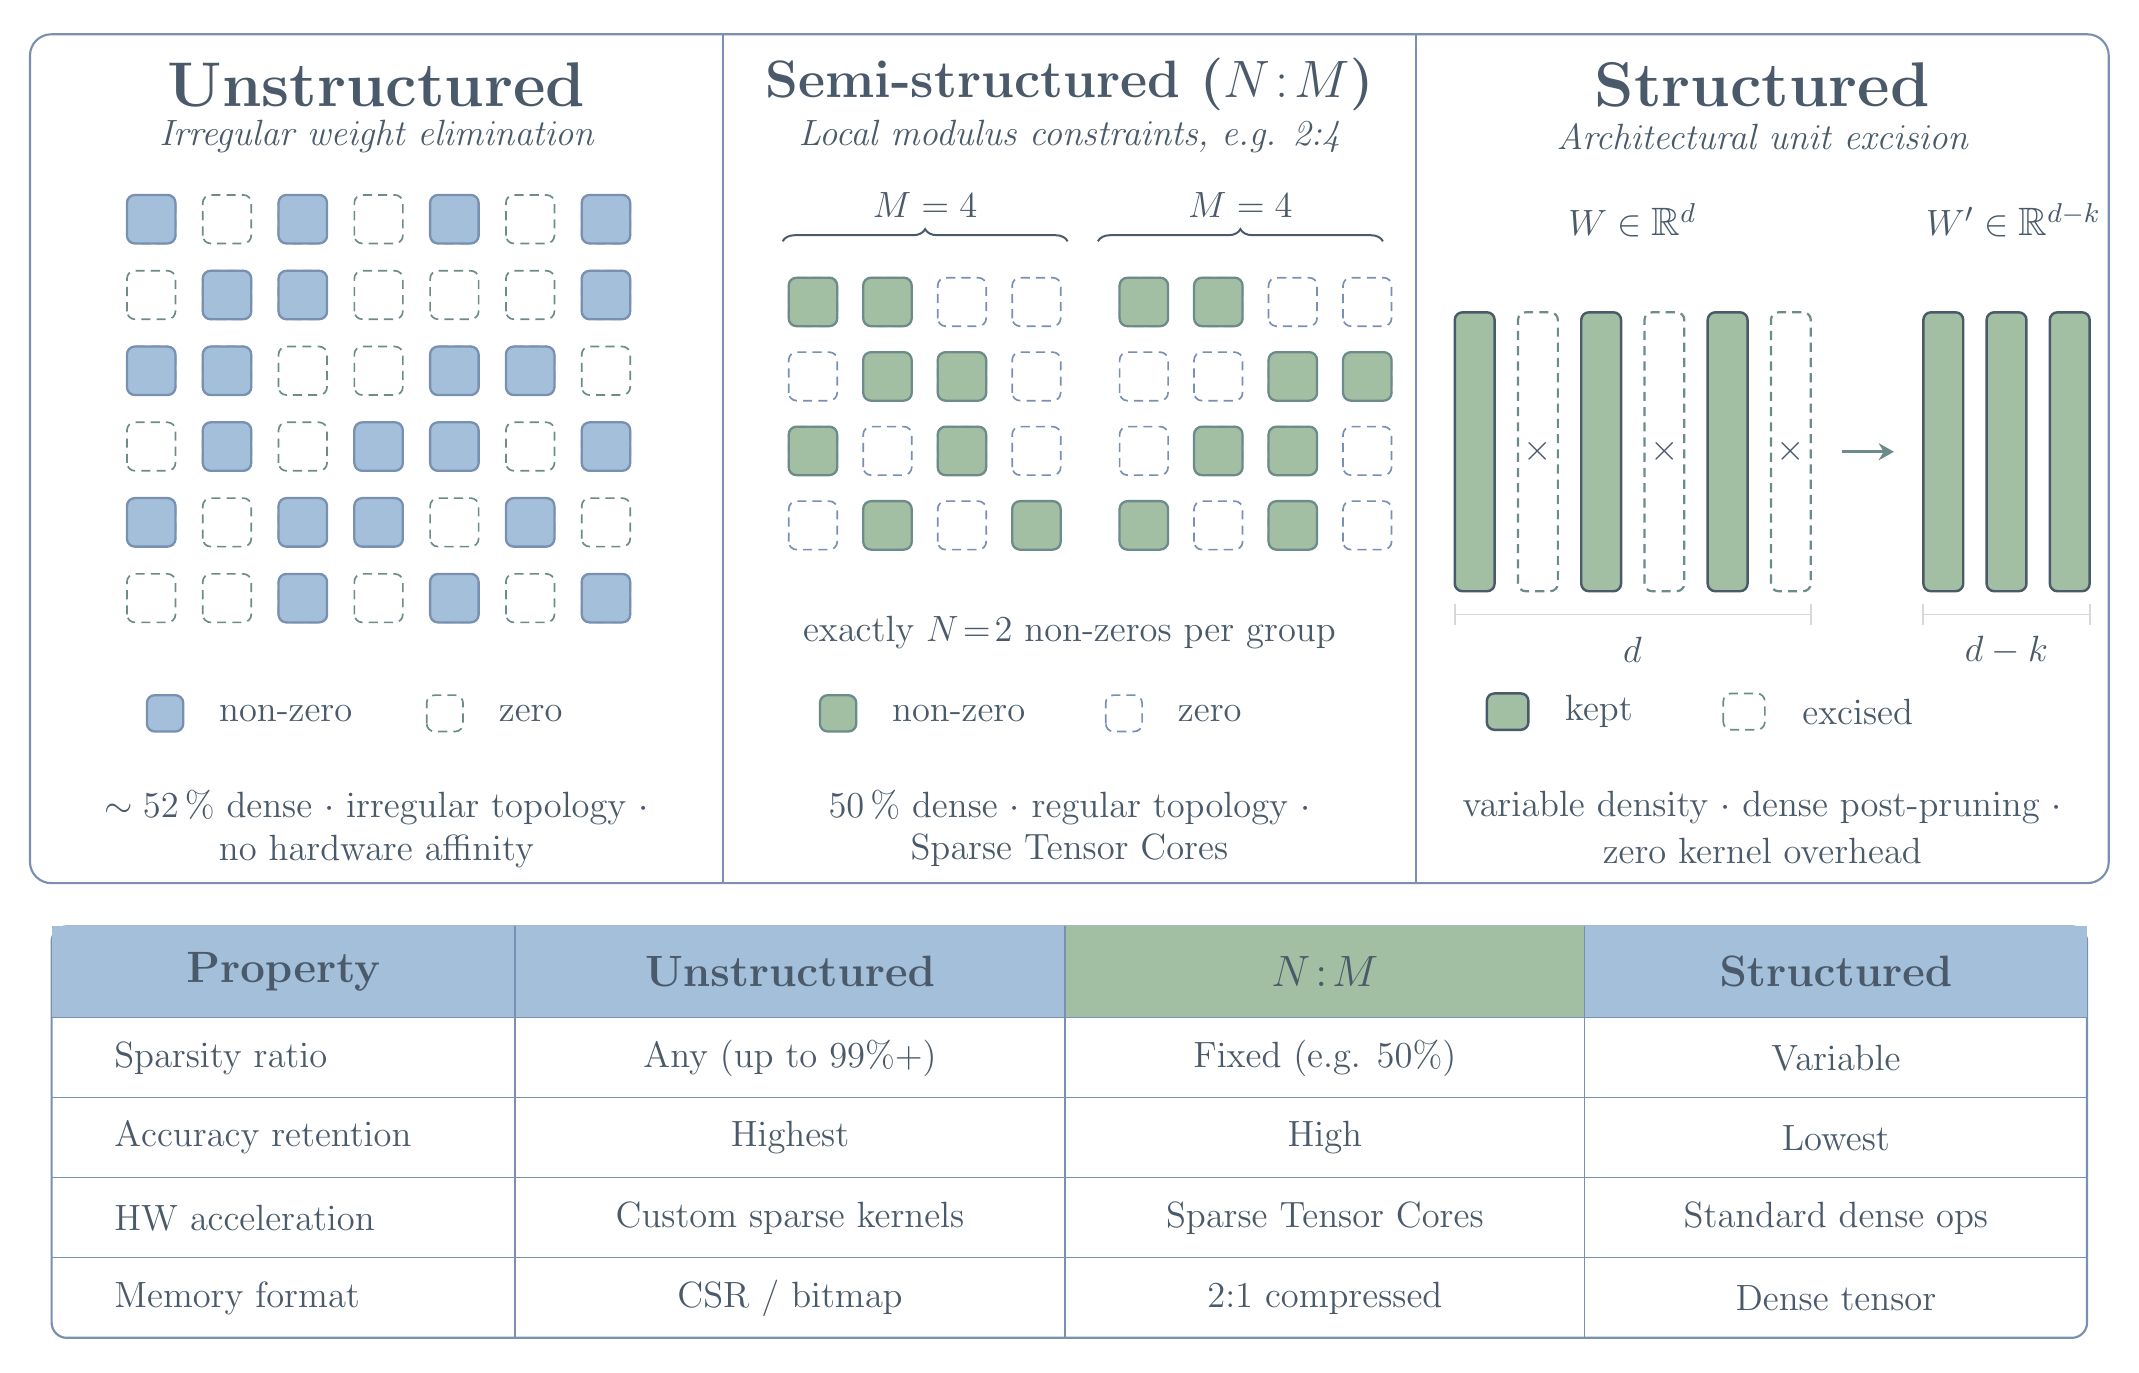
\includegraphics[width=\textwidth]{figures/compression/pruning_s_ss_ns.PNG}
	\caption{Comparison of unstructured, semi-structured, and structured sparsity
		patterns in a weight matrix.
%	White cells indicate removed weights. Unstructured
%		sparsity scatters zeros freely across the matrix; semi-structured sparsity
%		enforces a fixed retention ratio within each local group; structured sparsity
%		removes entire rows or columns, yielding a dense submatrix.
	}
	\label{fig:structures}
\end{figure}

%% ----------------------------------------------------------------------------
\section{Pruning Criteria}
\label{sec:pruning_criteria}

While the sparsity structure determines the shape and hardware footprint of the
compressed model, it says nothing about \emph{which} specific weights or units
should be removed. That decision is governed by the pruning criterion: given a
fixed removal budget, the criterion ranks the parameters or structures by their
estimated importance to the network's output, so that the least important ones
are removed first.
%% ----------------------------------------------------------------------------

A \keyterm{pruning criterion} assigns an importance score $S(\theta_i)$ (or
$S(g)$ for a structured group $g$) that serves as a proxy for the loss change
$\Delta\mathcal{L}$ induced by removing that element.  The ideal criterion
ranks units by \emph{true irreplaceability}: the unit with the lowest true
loss impact should be removed first.

\subsection{Magnitude-Based Criteria}
\label{subsec:magnitude_based_criteria}

The most common zeroth-order criterion evaluates a weight by its absolute value \cite{han2015learning}:
\begin{equation}
	S_{\mathrm{mag}}(w_i) = |w_i|.
	\label{eq:mag}
\end{equation}
For structured groups (e.g.\ a convolutional filter
$W_g \in \R^{c_\mathrm{out} \times c_\mathrm{in} \times k \times k}$), the
same idea is applied to the whole group rather than to one scalar weight. Common choices are the $\ell_1$, $\ell_2$, and $\ell_\infty$ norms:
\begin{align}
	S_g^{(1)} &= \norm{W_g}_1 = \sum_{i} |w_{g,i}|, \label{eq:mag_l1} \\
	S_g^{(2)} &= \norm{W_g}_2 = \sqrt{\sum_{i} w_{g,i}^2}, \label{eq:mag_l2} \\
	S_g^{(\infty)} &= \norm{W_g}_\infty = \max_i |w_{g,i}|. \label{eq:mag_linf}
\end{align}
These group scores extend the scalar magnitude rule to structured units: first score a whole tensor, then remove the groups with the smallest values. The $\ell_1$ score measures total absolute magnitude, the $\ell_2$ score measures Euclidean energy, and the $\ell_\infty$ score keeps only the largest entry in the group (Eqs.~\eqref{eq:mag}, \eqref{eq:mag_l1}, \eqref{eq:mag_l2}, and~\eqref{eq:mag_linf}).

The $\ell_2$ norm is the most common because it is differentiable and
rotation-invariant.  The $\ell_\infty$ norm is sensitive to outliers and
is less often used alone.

\textbf{Interpretation.} At a stationary point with a well-conditioned
Hessian, $S_{\mathrm{2nd}} = \tfrac{1}{2} H_{ii} w_i^2 \propto w_i^2$ if
$H_{ii}$ is approximately constant across parameters.  Under this assumption,
ranking by $|w_i|$ is equivalent to ranking by the second-order saliency \cite{lecun1989optimal}.
When Hessian diagonal entries vary greatly across layers (which they do in
practice), magnitude alone may rank units from poorly-conditioned layers too
aggressively.

\subsection{Gradient-Based Criteria}
\label{subsec:gradient_based_criteria}

First-order saliency estimates include the effect of the local gradient \cite{molchanov2017variational}:
\begin{equation}
	S_{\mathrm{grad}}(w_i)
	= \left|\frac{\partial\mathcal{L}}{\partial w_i}\cdot w_i\right|.
	\label{eq:grad}
\end{equation}
This is obtained from the first-order Taylor term with $\delta w_i = -w_i$
(complete removal), which turns the local gradient into a gradient-weight saliency score (Eq.~\eqref{eq:grad}). For structured pruning, the same criterion can be
extended to a removable group by summing over all constituent parameters:
\begin{equation}
	S_{\mathrm{grad}}(g)
	= \left|\sum_{i \in g}\frac{\partial\mathcal{L}}{\partial w_i}\cdot w_i\right|.
	\label{eq:grad_group}
\end{equation}
This produces one importance value for the whole group, not one value per scalar weight (Eq.~\eqref{eq:grad_group}) \cite{molchanov2017variational}.

\subsection{Second-Order Criteria}
\label{subsec:second_order_criteria}
For second-order criteria, the Taylor expansion is kept to the curvature term, which gives a more accurate estimate of the loss change but requires approximating the Hessian. The original OBD criterion is a simple diagonal approximation, while later methods apply the same idea blockwise to recover tractability.
There are two main approaches to second-order criteria: the diagonal approximation of OBD and the blockwise inverse Hessian of OBS.

\paragraph{Diagonal approximation (OBD style).}
\begin{equation}
	S_{\mathrm{2nd}}(w_i) = \frac{1}{2}\,H_{ii}\,w_i^2.
	\label{eq:second_order}
\end{equation}
The diagonal curvature term used in this score can be estimated from the Gauss-Newton approximation to the Hessian,
which requires computing per-sample gradients:
\begin{equation}
	H \approx G^\top G, \qquad G_{ij} = \frac{\partial \ell_j}{\partial w_i},
\end{equation}
where $\ell_j$ is the loss on sample $j$. The diagonal is then
$H_{ii} \approx \sum_j G_{ij}^2$, giving the curvature factor used by the second-order score (Eq.~\eqref{eq:second_order}).

\paragraph{Blockwise inverse Hessian.}
The full OBS correction is too expensive to apply to all parameters at once, so modern methods apply the same idea locally inside large linear layers \cite{hassibi1993second,frantar2023sparsegpt}. In a layer with weight matrix $W \in \R^{m \times n}$, the calibration activations are collected in $X \in \R^{n \times N}$, with one column per calibration sample. These activations give the empirical input Hessian $\hat{H}=XX^\top/N$, which describes how input directions interact inside the layer. The layer is then processed column by column: when one weight is removed, the remaining weights in the current block are adjusted so that the layer output changes as little as possible.
\begin{equation}
	W_{:,j}' = W_{:,j} - \frac{w_{:,j}}{[\hat{H}^{-1}]_{jj}}\, w_{:,j}^\top \hat{H}^{-1}_{j+1:, j},
	\label{eq:sparsegpt}
\end{equation}
This correction, written in Eq.~\eqref{eq:sparsegpt}, carries the pruning error into the surviving columns instead of leaving it concentrated at the removed weight. After each removal, the remaining inverse Hessian is updated efficiently, so the next pruning decision is made with the current block state rather than the original dense one. The total cost is $O(n^3 + mn^2)$ per layer.

\subsection{Activation-Aware Criteria}
\label{subsec:activation_aware_criteria}

Some criteria scale saliency by the activation statistics at the weight's
input. Concretely, the weight magnitude is multiplied by the $\ell_2$ norm of
the input feature it processes \cite{sun2023simple}:
\begin{equation}
	S_{\mathrm{act}}(W_{i,j}) = |W_{i,j}|\cdot\norm{x_j}_2,
	\label{eq:wanda}
\end{equation}
where $\norm{x_j}_2$ is the $\ell_2$ norm of the $j$-th input feature
computed over a calibration set of $N$ samples calculated as shown in Eq.~\eqref{eq:rms_activation}:
\begin{equation}
	\label{eq:rms_activation}
	\norm{x_j}_2 = \sqrt{\sum_{s=1}^{N} x_{s,j}^2\,}.
\end{equation}
This equals $\sqrt{N}$ times the root-mean-square (RMS) of that feature's
activations. RMS measures how much energy a feature carries on average
across inputs. A feature with consistently large activations has high RMS.
One that is rarely triggered has low RMS and contributes little to the
output regardless of its associated weight's magnitude. Equation~\eqref{eq:wanda}
makes the criterion sensitive to both: a small weight on a high-RMS feature
scores higher than a larger weight on a near-silent one.

Activation magnitudes are distributed unevenly across input features
\cite{sun2023simple,wei2022outlier}. Magnitude-only scoring ignores this.
It assigns identical importance to a weight on a high-energy feature and to
an equally large weight on a near-zero feature, systematically
underestimating the contribution of the first group. Scaling by
$\norm{x_j}_2$ corrects that bias directly.

\subsection{Learnable and Adaptive Criteria}
\label{subsec:learnable_adaptive_criteria}

A fourth family introduces \emph{trainable mask scores} $v \in \R^P$ that are optimised jointly with weights \cite{louizos2018learning,mallya2018packnet}:
\begin{equation}
	M_i = \sigma\!\left(\frac{v_i - \bar{v}}{\epsilon}\right),
	\quad
	\text{or}
	\quad
	M_i = \mathbf{1}[v_i \ge \tau],
	\label{eq:learnable}
\end{equation}
The mask can be kept soft during training or converted into a hard keep/remove decision (Eq.~\eqref{eq:learnable}). The discrete threshold is approximated during backpropagation by a straight-through estimator \cite{bengio2013estimating}, which passes the gradient through the threshold as if it were the identity. The learning objective then adds a sparsity penalty so that accurate but dense masks are discouraged:
\begin{equation}
	\mathcal{L}_{\mathrm{sparse}} = \mathcal{L}(\Theta, M(v)) + \lambda \norm{v}_1.
	\label{eq:learnable_loss}
\end{equation}
This objective balances task performance against mask sparsity (Eq.~\eqref{eq:learnable_loss}).

These approaches are valuable especially in the setting where the training
distribution is accessible and the budget for mask optimisation is not the
constraint. At moderate sparsities in fine-tuning, they outperform static
criteria \cite{sanh2020movement,louizos2018learning}.

\subsection{Criterion Comparison}
\label{subsec:criterion_comparison}

Table~\ref{tab:criterion_comparison} places the criteria of this section side by
side. Read from top to bottom, it traces a single trade-off: the cheaper
criteria near the top observe only the weights themselves, while the richer ones
below require gradients, curvature, activations, or a training signal. That extra
information is precisely what buys the accuracy gains in the last column. The
table is therefore best read as a map from \emph{what a criterion is allowed to
observe} to \emph{how well it ranks units for removal}, which is the trade-off a
practitioner balances against the available data and compute budget.

\begin{table}[H]
	\centering
	\caption{Summary comparison of pruning criteria.}
	\label{tab:criterion_comparison}
	\renewcommand{\arraystretch}{1.5}
	\begin{tabularx}{\textwidth}{lXXccl}
		\toprule
		\textbf{Criterion} & \textbf{Information used}
		& \textbf{Data needed}
		& \textbf{Grad?} & \textbf{$H$?}
		& \textbf{Typical accuracy} \\
		\midrule
		Magnitude & Weight values only
		& None & No & No & Baseline \\
		Gradient (Taylor) & Gradient $\times$ weight
		& Train/calib & Yes & No & +1--3\% over mag \\
		OBD (\S\ref{subsec:obd_obs}) & Diag.\ curvature
		& Train/calib & Yes & Diag & +1--5\% over mag \\
		Blockwise OBS (\S\ref{subsec:second_order_criteria}) & Full curvature per layer
		& Calibration & No & Block & Best (post-train) \\
		Activation-weighted & Magnitude $\times$ activation
		& Calibration & No & No & Strong post-train \\
		Learned / trajectory mask & Score trajectory
		& Fine-tune & Yes & No & Best for fine-tune \\
		\bottomrule
	\end{tabularx}
\end{table}

%% ----------------------------------------------------------------------------
\section{Pruning Strategies}
\label{sec:pruning_strategies}
%% ----------------------------------------------------------------------------

The criteria defined above state \emph{what} to remove. A related question is
\emph{when} this removal occurs and when to let the model recover in between
removals. A pruning schedule describes the pattern of mask updates and
recoveries during the course of training or preparing for inference, which is
what this section covers.

\subsection{One-Shot Pruning}
\label{subsec:one_shot_pruning}

In \keyterm{one-shot pruning}, importance scores are computed once from the
fully trained model and all removal decisions are made in a single pass
\cite{han2015deep}. Algorithm~\ref{alg:one_shot} shows the procedure.

\begin{algorithm}[H]
	\SetAlgoLined
	\KwIn{Trained model $f(\cdot;\Theta)$, target density $\kappa$}
	\KwOut{Pruned model $f(\cdot; M \odot \Theta)$}
	Compute $S(\theta_i)$ for all $i \in [P]$\;
	Set threshold $\tau \leftarrow$ $(1-\kappa)$ quantile of $\{S(\theta_i)\}$\;
	$M_i \leftarrow \mathbf{1}[S(\theta_i) \ge \tau]$\;
	\textbf{Optional:} fine-tune $\Theta$ with $M$ fixed\;
	\Return $M \odot \Theta$\;
	\caption{One-Shot Pruning}
	\label{alg:one_shot}
\end{algorithm}

One-shot pruning requires no additional training rounds and can be applied
directly to a pretrained model, which makes it simple to run. But that
simplicity has a cost. All removal decisions come from a single pass over the
loss landscape on a small calibration set, with no opportunity for the model
to recover between mask updates. Accuracy at a given sparsity is lower than
for iterative methods \cite{han2015deep,zhu2018prune}.

\subsection{Iterative Pruning and Recovery}
\label{subsec:iterative_pruning}

\keyterm{Iterative pruning} directly addresses the limitation of one-shot
pruning by interleaving mask updates with weight recovery steps \cite{zhu2018prune}. Instead of removing
all targeted weights at once, the model is pruned gradually over $R$ rounds,
with a fine-tuning phase after each round to let the remaining weights
compensate for what was removed. Algorithm~\ref{alg:iterative} shows a
common formulation using a cubic sparsity schedule.

\begin{algorithm}[H]
	\SetAlgoLined
	\KwIn{Trained model $\Theta$, target density $\kappa$, rounds $R$}
	\KwOut{Pruned model $M \odot \Theta$}
	$\kappa_0 \leftarrow 1.0$ \tcp*{start fully dense}
	\For{$r = 1$ \KwTo $R$}{
		$\kappa_r \leftarrow \textsc{Schedule}(\kappa,\, r,\, R)$ \tcp*{interpolate density toward target}
		Compute scores $S(\theta_i)$ on current $\Theta$ \tcp*{re-evaluate importance}
		Update mask $M$ to density $\kappa_r$ \tcp*{remove lowest-scoring units}
		Fine-tune $\Theta$ with $M$ fixed for $T_r$ steps \tcp*{recover accuracy}
	}
	\Return $M \odot \Theta$\;
	\caption{Iterative Pruning}
	\label{alg:iterative}
\end{algorithm}

The $\textsc{Schedule}$ function can take many forms such as linear, cubic,
cosine, or step, and the choice is often borrowed directly from learning
rate scheduling practice, since both problems share the same goal of
controlling how aggressively a quantity changes over the course of training
\cite{zhu2018prune}. Figure~\ref{fig:schedules} illustrates several common
variants.

\begin{figure}[H]
	\centering
	\begin{tikzpicture}
		\begin{axis}[
			width=0.92\linewidth, height=5.5cm,
			xlabel={Round ($r/R$)},
			ylabel={Sparsity $s_r$ (\%)},
			xmin=0, xmax=1, ymin=0, ymax=95,
			legend pos=south east,
			legend style={font=\small},
			grid=both, grid style={gray!15},
			xtick={0,0.25,0.5,0.75,1.0},
			ytick={0,20,40,60,80,90},
			title={Sparsity Schedules for Iterative Pruning ($\kappa = 0.10$)},
			title style={font=\small\bfseries},
			]
			\addplot[very thick, colBlueBorder, domain=0:1, samples=50]
			{90 * x};
			\addlegendentry{Linear}
			\addplot[very thick, headergreen, domain=0:1, samples=50]
			{90 * (1 - (1-x)^3)};
			\addlegendentry{Cubic (front-loaded)}
			\addplot[very thick, actreddark, const plot]
			coordinates {(0,0)(0.2,30)(0.4,60)(0.6,75)(0.8,85)(0.9,90)(1,90)};
			\addlegendentry{Step}
			\addplot[very thick, slateblue, domain=0:1, samples=50]
			{90 * 0.5 * (1 - cos(deg(pi * x)))};
			\addlegendentry{Cosine}
		\end{axis}
	\end{tikzpicture}
	\caption{ Variants of sparsity schedules}
%		Sparsity schedules for iterative pruning targeting 90\% sparsity
%		over $R$ rounds. Cubic and cosine schedules slow down near the target,
%		giving the model time to stabilise before the final mask is frozen;
%		linear and step schedules do not.}
	\label{fig:schedules}
\end{figure}

Linear growth applies equal increments each round, so the removal rate at
the end of training is the same as at the start, with no settling period at
high sparsity.
Cubic growth concentrates most of the pruning early: by $r/R = 0.5$ roughly
87\% of the target sparsity budget is already spent, and the remaining rounds
operate at near-final density with small incremental changes.
Step schedules skip continuous interpolation and instead apply discrete jumps
at fixed intervals, holding the mask constant between updates.
Cosine growth starts slowly and accelerates toward the midpoint, then
decelerates as sparsity approaches the target.
The last rounds under cosine resemble those of cubic. Both avoid committing
large removals at high sparsity, where each pruned weight carries a larger
marginal effect on the loss \cite{zhu2018prune}.

\subsection{Pruning During Training}
\label{subsec:pruning_during_training}

A third family integrates sparsity directly into the optimisation loop by
adding a regularisation term to the training loss, typically an $\ell_1$
penalty of the form $\lambda \sum_i |\theta_i|$ \cite{liu2017learning}.
This encourages weights toward zero throughout training, so that sparsity
emerges gradually rather than being imposed after the fact \cite{han2015deep,guo2016dynamic}. Weights that fall
below a threshold are later hard-pruned. The main requirement is access to
the full training distribution, which makes this approach most suitable when
training from scratch or during a supervised fine-tuning stage, rather than
for post-hoc compression of a frozen model.

\subsection{Post-Training Pruning}
\label{sec:post_training_pruning}

\keyterm{Post-training pruning} applies pruning to a frozen pretrained model
using only a small calibration set, without any gradient updates to the
original training loss \cite{frantar2023sparsegpt}. This makes it the
practical default for large pretrained networks, where full retraining over
the original training distribution is prohibitively expensive.

The procedure runs in four steps. First, a small calibration set of a few
hundred samples is forwarded through the frozen model to collect
layer-wise input activation statistics. Second, those statistics are combined
with the weight values to compute a saliency score $S(\theta_i)$ for each
weight or group. Third, the lowest-scoring units are zeroed out to produce
the binary mask $M^*$. Fourth, an optional weight correction step adjusts
the values of the remaining weights in each layer to compensate for the
damage caused by the removals, an idea inherited from OBS and applied
blockwise in modern post-training methods \cite{frantar2023sparsegpt}.
Figure~\ref{fig:ptp_pipeline} summarises these steps.

\begin{figure}[H]
	\centering
	\begin{adjustbox}{max width=\linewidth}
	\begin{tikzpicture}[
		font=\small,
		box/.style={rectangle, rounded corners=3pt, draw=colBlueBorder, fill=colBlue!15,
			minimum width=2.8cm, minimum height=0.7cm, align=center},
		data/.style={rectangle, rounded corners=3pt, draw=headergreen, fill=colGreen!25,
			minimum width=2.8cm, minimum height=0.7cm, align=center},
		arr/.style={-Stealth, thick, colBlueBorder}
		]
		\node[data]  (pretrain)   {Pretrained\\model $\Theta^*$};
		\node[data, below=0.5cm of pretrain] (calib)
		{Calibration\\set ($\le$512 samples)};
		\node[box, right=1.2cm of calib]  (stats)
		{Collect input\\activations\\per layer};
		\node[box, right=0.8cm of stats]  (score)
		{Compute saliency\\score $S(\theta_i)$\\per weight/group};
		\node[box, right=0.8cm of score]  (mask)
		{Zero out\\lowest-scoring\\units: mask $M^*$};
		\node[box, right=0.8cm of mask]   (opt)
		{Correct remaining\\weights to offset\\removed units};
		\node[data, below=0.7cm of opt]   (pruned)
		{Pruned model\\$M^* \odot \Theta^*$};

		\draw[arr] (pretrain) -| (stats);
		\draw[arr] (calib)    -- (stats);
		\draw[arr] (stats)    -- (score);
		\draw[arr] (score)    -- (mask);
		\draw[arr] (mask)     -- (opt);
		\draw[arr] (opt)      -- (pruned);
	\end{tikzpicture}
	\end{adjustbox}
	\caption{Post-training pruning pipeline.
%	A small calibration set is forwarded
%		through the frozen model to collect layer-wise activation statistics. These
%		are used to score each weight or group, after which the lowest-scoring units
%		are zeroed out. An optional weight correction step adjusts the remaining
%		weights to compensate for the removed ones. No
%		gradient update to the pretraining loss is performed at any stage.
	}
	\label{fig:ptp_pipeline}
\end{figure}


%% ----------------------------------------------------------------------------
So far, we have described pruning by means of three components: what structure should be eliminated, according to which evaluation measure, and which application strategy should be adopted. Because our specific interest is Transformers, these components now have to be identified within the architecture being compressed. In the next section, we therefore describe an instantiation of the pruning approach within Transformer models.

\section{Pruning Transformers}
\label{sec:pruning_transformers}
%% ----------------------------------------------------------------------------

The general framework described so far identifies three decisions: which
units to remove, by what criterion, and according to which schedule. Applying
this to a Transformer means mapping each decision to the specific computational
structures of the architecture. The three main removable units are attention
heads, FFN channels, and entire Transformer layers. Each carries a different
cost and requires a different adaptation of the pruning formulas.

\subsection{Attention Head Pruning}
\label{subsec:attention_head_pruning}

The multi-head attention module computes attention in $H$ parallel subspaces
called heads. Given an input sequence $X \in \R^{n \times d}$, where $n$ is
the sequence length and $d$ is the model dimension, each head $h$ projects $X$
into query, key, and value spaces of dimension $d_h = d/H$ using learned
matrices $W_{Q_h}, W_{K_h}, W_{V_h} \in \R^{d \times d_h}$, computes scaled
dot-product attention, and feeds the result through the shared output
projection $W_O \in \R^{d \times d}$.

A head mask $m \in \{0,1\}^H$ selects which of the $H$ heads contribute to
the output:
\begin{equation}
	\mathrm{MHA}_m(X) = \mathrm{Concat}(m_1\,\mathrm{head}_1(X), \ldots,
	m_H\,\mathrm{head}_H(X))\,W_O.
	\label{eq:mha_masked}
\end{equation}
Setting $m_h = 0$ zeros out $W_{Q_h}$, $W_{K_h}$, $W_{V_h}$, and the
corresponding block of columns in $W_O$ (Eq.~\eqref{eq:mha_masked}). Since each head uses query, key, value, and output projections, the number of parameters removed per
head is:
\begin{equation}
	\Delta P_{\mathrm{head}} = 4\,d\,d_h = \frac{4d^2}{H}.
	\label{eq:head_params}
\end{equation}

Early work on head importance found that a large share of heads can be removed
with no statistically significant drop in performance \cite{michel2022not,voita2019analyzing}.
Heads that carry out identifiable functions, such as attending to adjacent
tokens or tracking syntactic dependencies, are harder to remove, while heads
whose attention patterns closely resemble those of other heads in the same
layer are the most dispensable \cite{voita2019analyzing}. Importance varies
considerably across layers and no single head is universally critical
\cite{michel2022not}.

\subsection{FFN Channel Pruning}
\label{subsec:ffn_channel_pruning}

The feed-forward network in each Transformer layer expands the model dimension
by a factor $r$ before projecting back. For an input $X \in \R^{n \times d}$
and expansion ratio $r$, the standard FFN applies:
\begin{equation}
	\mathrm{FFN}(X) = \phi(X W_1 + b_1)\,W_2 + b_2,
	\label{eq:ffn_base}
\end{equation}
where $W_1 \in \R^{d \times rd}$, $W_2 \in \R^{rd \times d}$, and $\phi$ is
a pointwise activation function. This is the standard two-projection FFN block used before channel pruning (Eq.~\eqref{eq:ffn_base}). A channel mask
$g \in \{0,1\}^{rd}$ selects which of the $rd$ intermediate neurons to retain:
\begin{equation}
	\mathrm{FFN}_g(X) = \phi(XW_1 + b_1)\,\mathrm{diag}(g)\,W_2 + b_2.
	\label{eq:ffn_masked}
\end{equation}
Writing $\mathcal{K} = \{k : g_k = 1\}$ for the retained channel indices,
the masked FFN can be rewritten as a dense FFN of smaller width:
\begin{equation}
	\mathrm{FFN}_g(X) = \phi(X W_{1,\mathcal{K}} + b_{1,\mathcal{K}})\,
	W_{2,\mathcal{K},:} + b_2.
	\label{eq:ffn_compact}
\end{equation}
Removing one channel eliminates one row of $W_1$ and one column of $W_2$,
which is exactly what the masked and compact forms express (Eqs.~\eqref{eq:ffn_masked} and~\eqref{eq:ffn_compact}). Each removed channel therefore saves $2d$ parameters. For
$rd - |\mathcal{K}|$ removed channels the total saving is
$(2d)(rd - |\mathcal{K}|)$.

\subsection{Layer Pruning}
\label{subsec:layer_pruning}

Each Transformer block is an additive function: $F_l(x) = x + F_l^{(1)}(x)$,
where $F_l^{(1)}(x)$ is the composition of the attention sub-layer and the
FFN sub-layer. When $F_l^{(1)}(x)$ is small relative to $x$, the residual
connection carries the bulk of the signal and the block contributes little to
the representation. Removing it leaves downstream activations largely
unchanged.

A natural way to measure this is to compare the magnitude of $F_l(x)$ to the
magnitude of the input $x$ over a calibration set. Using the Frobenius norm
$\|\cdot\|_F$ (the square root of the sum of all squared entries of a matrix)
as the measure of size, the relative block contribution is:
\begin{equation}
	S_l^{\mathrm{block}} = \frac{\|F_l(X)\|_F}{\|X\|_F},
	\label{eq:block_sensitivity}
\end{equation}
where the norms are computed over a batch of calibration inputs $X$. A block
with a small relative contribution is close to an identity map, so it becomes a natural candidate for removal (Eq.~\eqref{eq:block_sensitivity}) \cite{michel2022not,kurtic2023ziplm}.

Layer pruning has the coarsest effect of any structured pruning decision since
a single removal eliminates all parameters in one attention module and one FFN,
a far larger parameter count than removing a head or a set of channels. This
makes it effective for reducing inference latency, which scales with the number
of layers, but recovery through fine-tuning is generally needed when more than
a small number of layers are removed \cite{kurtic2023ziplm}.

\section{Conclusion}
\label{sec:pruning_chapter_conclusion}

The chapter formalized pruning as a constrained optimization problem, surveyed
the three structural sparsity regimes, and compared the saliency criteria from
magnitude scoring through second-order blockwise methods.
Section~\ref{sec:pruning_transformers} covers the Transformer instantiation.

\noindent Pruning strategy determines when the mask is updated and how much
recovery the model gets between removals. One-shot, iterative, training-time,
and post-training regimes each carry a different accuracy-cost profile, and
the choice matters as much as the criterion. Together these components provide
the vocabulary the method-level review in
Chapters~\ref{chap:related_work_pruning_unstructured} and ~\ref{chap:related_work_pruning_structured}
builds on.
%	\chapter{Related Work}
\label{chap:related_work_pruning}

\section{Introduction}

Chapter~\ref{chap:neural_network_pruning} established the formal pruning problem, the main sparsity
regimes, the dominant saliency criteria, and the Transformer structures that
can be removed in practice. Against this background, the pruning literature
may be read as a sequence of increasingly structured responses to the same
core problem: how to remove computation while preserving the behavior of the
reference model under explicit deployment constraints.

The literature is not homogeneous: some methods target weight-level sparsity,
others remove executable structures such as heads, FFN channels, or layers,
and others treat pruning as a constrained configuration-search problem under
hardware or latency objectives. The discussion is therefore organized by
pruning mechanism and interpreted with attention to the evaluation regime used
by each paper, since compression level alone is insufficient to compare methods
that optimize different units, use different recovery pipelines, or report
different forms of efficiency.

\section{Related Work on Pruning}
Pruning is the most widely studied form of model compression, and it has been applied to Transformers in a variety of ways. The related work discussion is organized along two coupled axes: the topology of the induced sparsity pattern and the optimization signal used to identify removable units. This framing keeps the deployment question explicit from the outset, because similar nominal compression ratios may correspond to different execution regimes, different preprocessing costs, and different forms of realized speedup.

\subsection{Problem Setting and Taxonomy}

\providecommand{\methoddetail}[1]{%
    \par\medskip
    \noindent{\bfseries #1}\par
    \smallskip\noindent
}
\providecommand{\methodsep}{%
    \par\smallskip
    \noindent\rule{0.28\textwidth}{0.35pt}
    \par\smallskip
}

Building on the formal framework introduced in Chapter~\ref{chap:neural_network_pruning}, the related-work discussion is organized along two coupled axes: the topology of the induced sparsity pattern and the optimization signal used to identify removable units.

\subsubsection{Taxonomy of Transformer Pruning Methods}

The main sparsity topologies were introduced formally in Section~\ref{sec:pruning_structures} (see Figure~\ref{fig:structures}). From a deployment standpoint, they differ in whether pruning yields compressed storage alone or native dense-shape acceleration after model surgery.

The taxonomy adopted here follows four coupled axes. The \emph{removable unit} determines whether the method acts on scalar weights or executable structures such as attention heads, FFN channels, and layers \cite{michel2022not,kurtic2022optimal}. The \emph{optimization signal} ranges from magnitude and activation statistics to differentiable mask learning, first-order Taylor criteria, second-order curvature surrogates, or search-based objectives \cite{sun2023simple,xia2022structured,ma2023llmpruner,frantar2023sparsegpt,kwon2022fast}. The \emph{recovery stage} distinguishes direct post-training pruning from methods requiring LoRA recovery, gradual fine-tuning, or distillation. The \emph{deployment objective} determines whether the reported benefit is compressed storage, dense-shape acceleration, or measured speedup \cite{kurtic2023ziplm,evopress2024,darwinlm2025}.

Each family corresponds to a different deployment objective. Unstructured methods such as Wanda and SparseGPT primarily optimize weight-level saliency \cite{sun2023simple,frantar2023sparsegpt}. Structured methods span differentiable mask-learning (CoFi), dependency-aware gradient methods (LLM-Pruner), Fisher-based post-training frameworks, and runtime-aware second-order methods (ZipLM) \cite{xia2022structured,ma2023llmpruner,kwon2022fast,kurtic2023ziplm}. Search-based methods such as EvoPress and DarwinLM treat pruning as configuration optimization under explicit budget or hardware constraints \cite{evopress2024,darwinlm2025}. Figure~\ref{fig:pruning_taxonomy} and Table~\ref{tab:pruning_taxonomy} summarize this organization.

\begin{figure}[p]
	\centering
	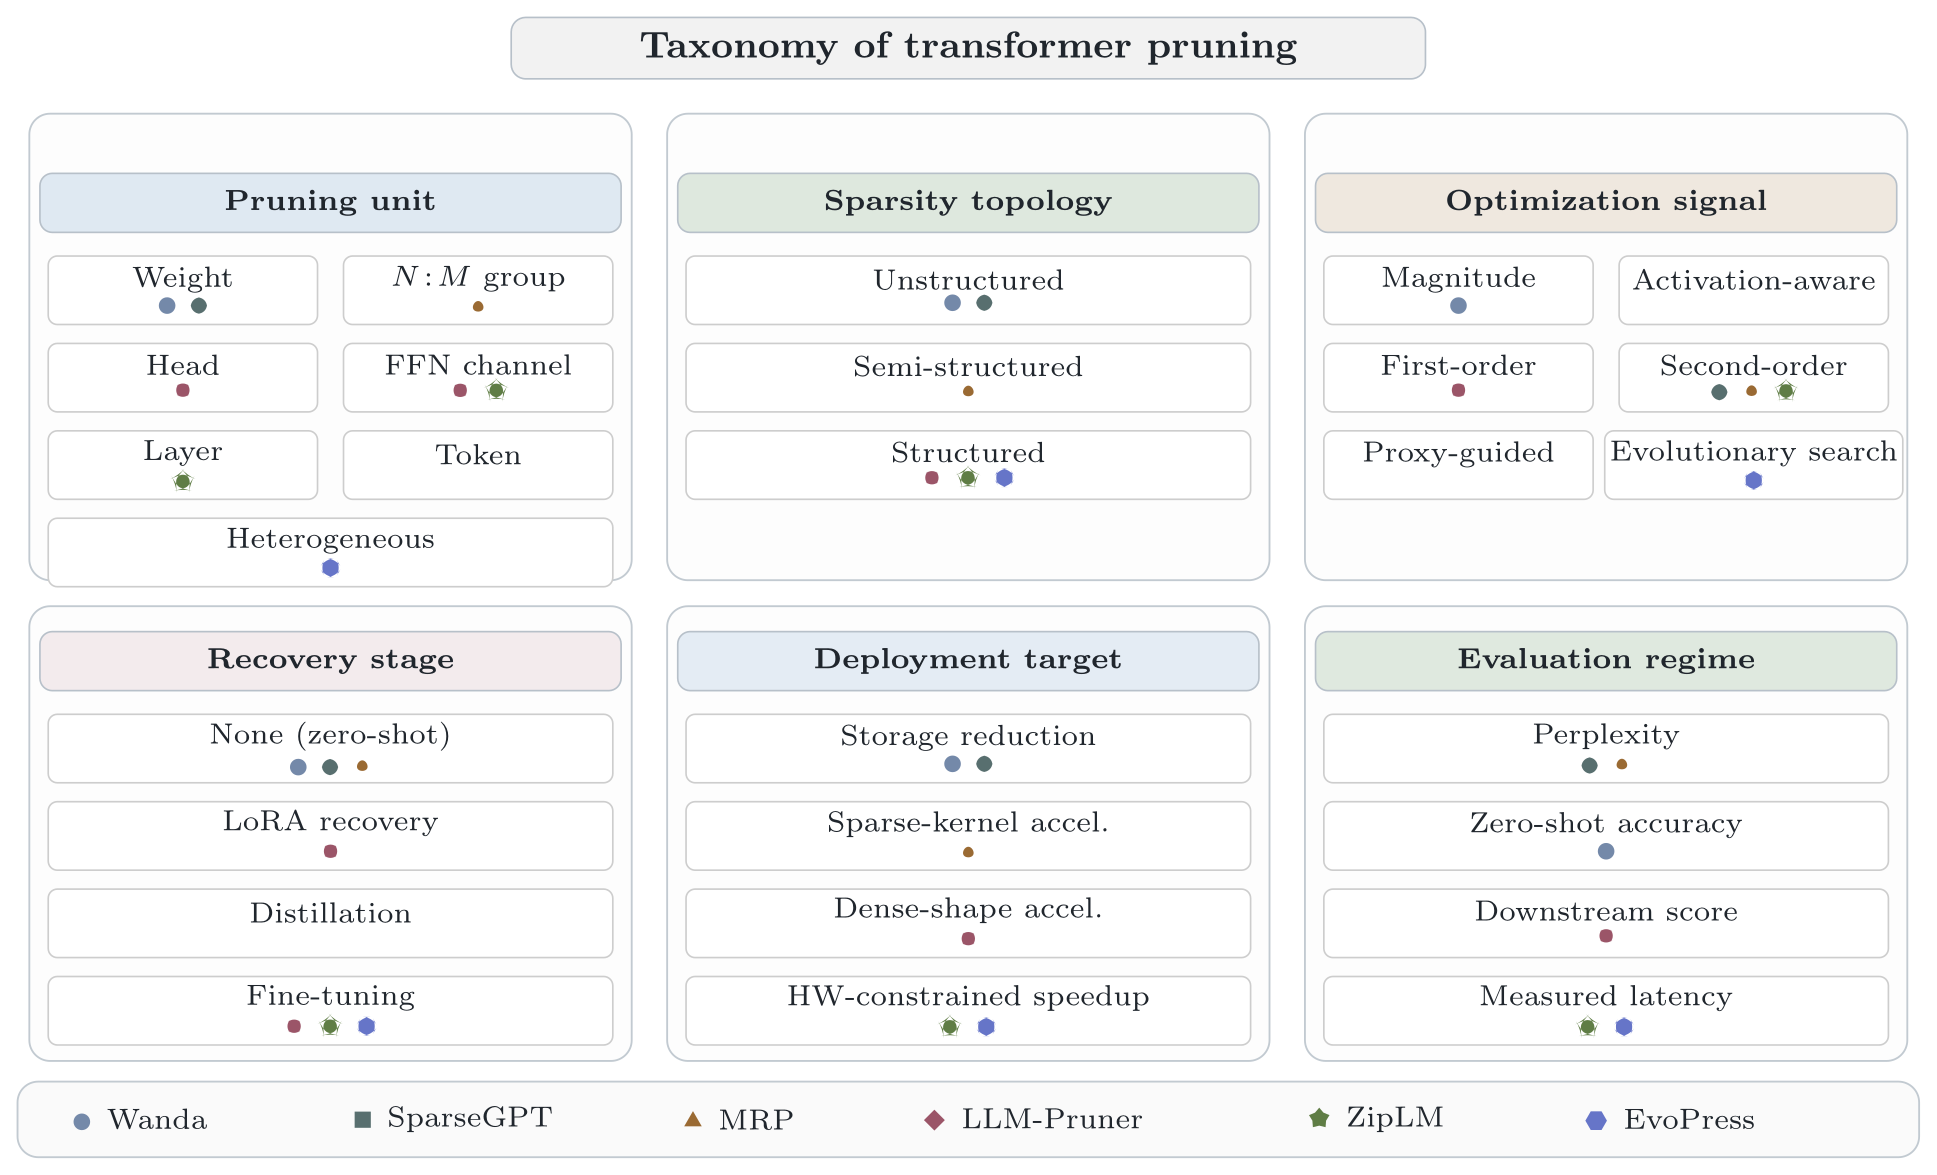
\includegraphics[width=\textwidth, height=0.88\textheight, keepaspectratio]{figures/compression/transformer_pruning_taxonomy.png}
	\caption{Taxonomy of the pruning methods considered in this chapter. The classification crosses the pruning unit, sparsity topology, optimization signal, recovery stage, deployment objective, and evaluation regime.}
	\label{fig:pruning_taxonomy}
\end{figure}

\begin{table}[H]
	\centering
	\caption{Taxonomy used to organize the pruning methods discussed in this chapter. The table distinguishes the removable unit, sparsity topology, optimization signal, recovery stage, and primary deployment claim for each method family.}
	\label{tab:pruning_taxonomy}
	\begin{tabularx}{\textwidth}{@{}l >{\raggedright\arraybackslash}X >{\raggedright\arraybackslash}X >{\raggedright\arraybackslash}X >{\raggedright\arraybackslash}X >{\raggedright\arraybackslash}X@{}}
		\toprule
		\textbf{Method} & \textbf{Unit} & \textbf{Topology} & \textbf{Signal} & \textbf{Recovery} & \textbf{Primary deployment claim} \\
		\midrule
		Wanda & Weight & Unstructured & Activation-aware saliency & None & Storage-oriented sparsity with strong zero-shot perplexity retention \\
		SparseGPT & Weight & Unstructured & Single-weight second-order compensation & None & High-sparsity pruning with local reconstruction \\
		CoFi & Layers / heads / FFN / hidden dimensions & Structured & Learned hard-concrete masks with $L_0$ control and distillation & Full task-specific pruning and fine-tuning & Dense-shape acceleration through jointly pruned Transformer structure \\
		LLM-Pruner & Heads / channels / blocks & Structured & First-order Taylor scoring with dependency groups & LoRA recovery & Structural compression with dense-shape execution \\
		Fast post-training pruning & Heads / FFN filters & Structured & Fisher-based constrained mask optimization & None beyond mask tuning & FLOPs- or latency-constrained structured pruning without retraining \\
		ZipLM & Heads / FFN dimensions & Structured & Second-order structured saliency with runtime-constrained search & Gradual fine-tuning and distillation & Measured speedup under device-specific constraints \\
		EvoPress / DarwinLM & Layer-wise compression levels & Heterogeneous structured & Proxy-guided or evolutionary search & Search-time evaluation or proxy training & Global configuration search under budget and hardware constraints \\
		\bottomrule
	\end{tabularx}
\end{table}

Figure~\ref{fig:pruning_taxonomy} should be read as a map of the chapter rather than as a ranking of methods. It separates the pruning literature by the kind of object being removed and by the signal used to decide removal. Table~\ref{tab:pruning_taxonomy} then makes this map concrete by assigning each reviewed method to a pruning unit, topology, scoring mechanism, recovery regime, and deployment claim.

The following subsections use this organization to review the selected pruning families in sequence: saliency-based methods, gradient-based structured methods, second-order methods, and search-based methods.

\clearpage
\subsection{Saliency-Based Methods}

Recall from Section~\ref{sec:pruning_criteria} that the Taylor expansion of the
loss change induced by pruning a weight $\theta_i$ produces a first-order term
proportional to the gradient and a second-order term capturing curvature
(Equation~\eqref{eq:taylor}). Saliency-based methods discard both terms and
instead use the weight magnitude or a proxy derived from activation statistics
as a surrogate for the true loss change. This zeroth-order approximation
requires no gradient computation and no calibration beyond a simple forward
pass, making these methods the cheapest option in the taxonomy.

\subsubsection{Magnitude and Activation-Aware Baselines}

\paragraph{Weight-Magnitude Pruning.}
Magnitude pruning uses absolute weight values as the saliency proxy:
\begin{equation}
	\mathcal{S}^{\mathrm{mag}}_{i,j} = |W_{i,j}|.
\end{equation}
Its core assumption is that small weights contribute less to the output and can be removed with limited degradation. The method requires no gradient-based recovery and remains the simplest baseline against which more sophisticated algorithms are evaluated.

\methodsep

\paragraph{Wanda (Weights $\times$ Activations).}
Wanda \cite{sun2023simple} refines this baseline by incorporating activation information from a small calibration set. The saliency score is
\begin{equation}
	\mathcal{S}^{\mathrm{wanda}}_{i,j} = |W_{i,j}| \cdot \|x_j\|_2,
\end{equation}
where $x_j$ is the $j$-th input activation channel and $\|x_j\|_2$ is its RMS norm estimated over $N$ calibration samples. The key insight is that importance is jointly encoded in weight magnitude and the energy of the coupled input channel.

\methoddetail{Algorithm Overview}
Both magnitude pruning and Wanda are one-shot post-training methods in the regime of Section~\ref{sec:post_training_pruning}: scores are computed once and no recovery training is applied afterward. Wanda processes each layer independently: it collects input activations on a small calibration set (typically 128 samples), computes per-weight saliency scores as the product of weight magnitude and activation norm, then prunes the lowest-scoring weights for each output neuron until the target sparsity $p$ is reached. No weight update or recovery step is applied. Magnitude pruning is a pure linear scan $O(|W|)$ with no calibration; Wanda adds only an activation-collection pass, keeping the overall cost near-linear.

These saliency methods are useful because they are cheap and easy to apply, but their decisions remain local. Once pruning moves from individual weights to heads, FFN channels, or layers, the method must account for structural dependencies between parameters. This motivates gradient-based structured pruning methods, where the score is computed over groups that can be removed consistently.

\subsection{Gradient-Based Methods}

Retaining the first-order term of the Taylor expansion (Equation~\eqref{eq:taylor}) gives a score proportional to the product of the gradient and the weight value. This makes the criterion sensitive to the direction of the loss landscape rather than just the weight magnitude, and it naturally extends to groups of weights by summing or aggregating the per-element scores. The methods in this section use exactly this first-order signal, applied to structured units such as heads, channels, and blocks rather than individual scalars.

Structured pruning replaces individual-weight saliency with group-level importance, because the natural units in a Transformer, namely attention heads, FFN channels, and entire layers, are coupled through residual pathways and shared projection matrices. Removing one head, for example, requires deleting consistent slices from $W_Q$, $W_K$, $W_V$, and $W_O$ together; removing an FFN channel removes coordinated rows and columns from the two projection matrices. Any pruning criterion applied at this level must therefore identify groups that can be removed as a unit without breaking the forward pass \cite{michel2022not,kurtic2022optimal}.

\paragraph{LLM-Pruner.}
LLM-Pruner \cite{ma2023llmpruner} addresses the dependency problem explicitly by constructing a graph over the neurons of the network. For neurons $N_i$ and $N_j$ with input set $\mathrm{In}(N)$ and output set $\mathrm{Out}(N)$, the graph encodes two rules:
\begin{align}
	N_j \in \mathrm{Out}(N_i) \wedge \deg^{-}(N_j)=1 &\implies N_j \text{ depends on } N_i, \label{eq:dep1}\\
	N_i \in \mathrm{In}(N_j) \wedge \deg^{+}(N_i)=1 &\implies N_i \text{ depends on } N_j. \label{eq:dep2}
\end{align}
Here $\deg^{-}(N_j)$ is the in-degree of $N_j$ (number of neurons feeding into it) and $\deg^{+}(N_i)$ is the out-degree of $N_i$. The transitive closure of these rules groups all coupled parameters into a single dependency group $\mathcal{G} = \{W_i\}_{i=1}^M$, which is the minimal unit that can be consistently removed.

Once groups are defined, each is scored using a first-order Taylor approximation of the loss increase over a small calibration set $\mathcal{D}$. The importance of a structure tensor $W_i$ is estimated as
\begin{equation}
	I_{W_i}
	\approx
	\left|
	\frac{\partial \mathcal{L}^{\top}(\mathcal{D})}{\partial W_i}W_i
	-\frac{1}{2}W_i^{\top}HW_i
	\right|,
	\label{eq:taylor-vector}
\end{equation}
where $H$ is the local Hessian. The first-order gradient is retained alongside the Hessian term because the calibration set is only a proxy for the pretraining distribution; discarding it would introduce bias. An element-wise variant replaces $H$ with a Fisher-diagonal approximation. Individual tensor scores within a group are aggregated by sum, product, max, or last-only operators, and groups with the lowest aggregate score are removed first.

LLM-Pruner sits between a post-training and a recovery regime: scoring is post-training and requires no gradient propagation through the full model, but the pruned network is then passed through a LoRA recovery stage in line with the iterative recovery approach of Section~\ref{subsec:iterative_pruning}. LoRA adapters \cite{hu2021lora} are inserted into all linear modules and fine-tuned for two epochs over roughly 50K samples. The low-rank factors are then merged back into the weight matrices, leaving no adapter overhead at inference time. The full scoring stage requires only 10 short calibration sequences, making the preprocessing cost modest relative to the recovery phase.

\methodsep

\paragraph{CoFi.}
CoFi \cite{xia2022structured} is the main structured-pruning example of the learnable-mask criteria introduced in Section~\ref{subsec:learnable_adaptive_criteria}. It places binary masks on attention blocks, heads, FFN blocks, intermediate channels, and the shared hidden dimension, then optimises these masks jointly with the task loss:
\begin{align}
	\mathrm{MHA}(X) &= z_{\mathrm{MHA}} \sum_{i=1}^{N_h} z_{\mathrm{head}}^{(i)} \,\mathrm{Att}\!\left(W_Q^{(i)},W_K^{(i)},W_V^{(i)},W_O^{(i)},X\right), \\
	\mathrm{FFN}(X) &= z_{\mathrm{FFN}}\, \mathrm{gelu}(XW_U)\,\mathrm{diag}(z_{\mathrm{int}})\,W_D,
\end{align}
where $N_h$ is the number of attention heads, $W_Q^{(i)}, W_K^{(i)}, W_V^{(i)}, W_O^{(i)}$ are the query, key, value, and output projection matrices of head $i$, and $W_U$, $W_D$ are the up- and down-projection matrices of the FFN. Each mask variable $z$ is relaxed to a continuous value during training using the hard-concrete distribution for $L_0$ regularisation, which allows gradients to flow through the mask. The training objective combines task loss with a distillation term and a Lagrangian sparsity constraint:
\begin{equation}
	\mathcal{L}_{\mathrm{prune}}
	=
	\mathcal{L}_{\mathrm{task}}
	+
	\mathcal{L}_{\mathrm{distil}}
	+
	\lambda_1(\hat s - s_0)
	+
	\lambda_2(\hat s - s_0)^2,
\end{equation}
where $s_0$ is the sparsity target and $\hat{s}$ is the expected sparsity under the current mask distribution. Because the masks at different granularities interact, CoFi can discover structured subnetworks that a simple per-group ranking would miss.

\methoddetail{Algorithm Overview}
CoFi is a training-time iterative method in the sense of Section~\ref{subsec:iterative_pruning}: mask decisions and weight updates are interleaved throughout training rather than applied once. A warm-up phase first stabilizes the model weights before mask learning begins, with the sparsity constraint applied softly. The main phase then jointly optimises masks and weights under the Lagrangian objective, progressively tightening the sparsity target toward $s_0$ over training. Once the target is reached, each continuous mask variable is thresholded against zero to produce a binary decision, and a final fine-tuning pass is run on the surviving subnetwork. Because masks at all granularities are trained simultaneously, the discovered subnetwork reflects cross-level interactions rather than independent per-unit decisions.

Gradient-based structured pruning improves the consistency of the removed units, but the score still depends on a local approximation of how removal affects the loss. When pruning becomes more aggressive, interactions among remaining and removed weights become more important. This leads to second-order methods, which use curvature information or local reconstruction objectives to compensate for the error introduced by pruning.

\subsection{Second-Order Methods}

The second-order term of the Taylor expansion (Equation~\eqref{eq:taylor})
captures the curvature of the loss around the current weights. Retaining this
term, rather than discarding it as saliency and gradient methods do, allows the
pruning criterion to account for how much a removal actually shifts the loss
given the local geometry of the loss landscape. As discussed in
Section~\ref{subsec:second_order_criteria}, this leads to the OBS framework,
where the optimal weight correction after a removal is derived from the inverse
Hessian. The methods in this section apply that same principle at the scale of
modern LLMs, recovering tractability by restricting the Hessian computation to
individual layers or column blocks.

\subsubsection{Optimal Brain Compression Formulation}

For a layer with weight matrix $\mathbf{W} \in \mathbb{R}^{d_{\text{out}} \times d_{\text{in}}}$ and calibration activations $\mathbf{X} \in \mathbb{R}^{d_{\text{in}} \times n}$, the layer-wise sparse reconstruction problem is
\begin{equation}
	\min_{\mathbf{W}^{\text{sparse}}}
	\|\mathbf{W}\mathbf{X} - \mathbf{W}^{\text{sparse}}\mathbf{X}\|_F^2
	\quad \text{s.t.} \quad
	\|\mathbf{W}^{\text{sparse}}\|_0 \leq (1-p)\, d_{\text{out}} d_{\text{in}},
\end{equation}
where $\|\cdot\|_F$ is the Frobenius norm, $\|\cdot\|_0$ counts the number of nonzero entries, and $p \in (0,1)$ is the target sparsity ratio. Using the empirical Hessian proxy $\mathbf{H} = \mathbf{X}\mathbf{X}^T / n$, this becomes a curvature-aware reconstruction problem whose solution depends on $\mathbf{H}^{-1}$ to redistribute pruning error across remaining weights. The methods that follow differ in how they instantiate this objective: SparseGPT removes one scalar weight at a time, MRP removes an entire N:M group jointly, Fisher-based pruning applies curvature scoring to structured masks, and ZipLM extends the same principle to executable Transformer structures under runtime constraints.

\subsubsection{Single-Weight Iterative Removal (SparseGPT)}

SparseGPT \cite{frantar2023sparsegpt} greedily prunes one weight at a time while applying compensation updates to remaining weights in the current block. This can be read as a blockwise version of the OBS correction introduced in Section~\ref{subsec:obd_obs} and formalised for large linear layers in Section~\ref{subsec:second_order_criteria}. Its local objective at iteration $t$ is
\begin{equation}\label{eq:srp}
	\min_{\delta w} \frac{1}{2}\delta w^T H \delta w
	\quad\text{s.t.}\quad
	(w+\delta w)\cdot e_t = 0,
\end{equation}
where $e_t$ is the one-hot selector for the pruned weight.

\methoddetail{Algorithm Overview}
SparseGPT is a post-training one-shot method in the regime of Section~\ref{sec:post_training_pruning}: pruning and compensation are applied in a single forward pass over the layers without any subsequent gradient-based recovery. It processes the weight matrix in column blocks of size $B$. For each block, it first constructs the regularized inverse Hessian $(XX^T + \lambda I)^{-1}$. Within each block, it iteratively identifies the weight with minimum local second-order loss, sets it to zero, then updates the remaining weights in that block using the corresponding column of $\mathbf{H}^{-1}$. After processing a block, lazy batch updates are applied to adjacent blocks. The method scales as $O(d_{\text{in}}^2 d_{\text{out}} + d_{\text{in}}^3/B)$ per layer, with a calibration budget of approximately 128 samples.

It is more instructive to understand SparseGPT as a weight-level, Hessian-compensated method for pruning: each decision to prune weights is made locally, and weights are updated to make the layer output's deviation as minimal as possible \cite{frantar2023sparsegpt}. It is through this same lens that SparseGPT's modification for semi-structured N:M sparsity can be understood, where the compensation method is kept and mask selection is constrained to local groups. If the block size is set to $B_s = M$, and from each group of $M$ weights the $N$ weights with the smallest OBS reconstruction score are selected for removal, the compensation becomes more localized to a block rather than the whole layer. Within that block, however, weights are still selected and compensated one at a time, so the compensation at each step does not account for the interactions among the other weights being simultaneously removed from the same group, which is the gap MRP directly addresses.

\methodsep

\subsubsection{Joint Optimization for Multi-Weight Removal (MRP)}

The MRP framework \cite{zhao2024pruning} generalizes second-order pruning to N:M groups. For a vectorized weight block $w$ and binary pruning mask $M$, where $M_i=1$ indicates that weight $i$ is pruned, the objective minimizes the second-order loss increase for the full group:
\begin{equation}\label{eq:ptp}
	\min_{\delta w} \frac{1}{2}\delta w^T H \delta w + g^T \delta w
	\quad\text{s.t.}\quad
	(w+\delta w)\odot M = 0,
\end{equation}
where $g$ is the gradient of the loss with respect to $w$, and $\odot$ denotes elementwise multiplication. Solving the group jointly yields a compensation update for the retained weights:
\begin{equation}
	\delta w^\star = -H_{\bar{M}\bar{M}}^{-1}(g_{\bar{M}} + H_{\bar{M}M}w_M),
\end{equation}
where $M$ denotes pruned indices, $\bar{M}$ retained indices, and $w_M$ the weight values at the pruned coordinates. This expression makes the role of the block Hessian explicit: in N:M pruning, the removed weights are not independent decisions, so compensation must be computed for the group rather than for a single scalar.

\methoddetail{Algorithm Overview}
MRP is a post-training one-shot method in the regime of Section~\ref{sec:post_training_pruning}: no gradient updates or recovery training are applied after pruning. It operates layer by layer. For each layer, the block Hessian is estimated from calibration activations. The weight tensor is partitioned into non-overlapping groups of $M$ consecutive weights. For each group, the joint second-order problem is solved: the mask selecting the $M-N$ weights with the highest reconstruction cost is identified, and the compensation update $\delta w^\star$ is applied to the retained $N$ weights before the next group is processed. Because the group is treated as a unit rather than a sequence of scalar removals, the method correctly accounts for interactions among simultaneously pruned coordinates within the block.

Figure~\ref{fig:hessian_compensation} illustrates this difference. SparseGPT compensates after removing one scalar weight, whereas MRP compensates after removing a constrained local group. The figure is therefore used to distinguish scalar second-order correction from group-level second-order correction.

\begin{figure}[H]
\centering
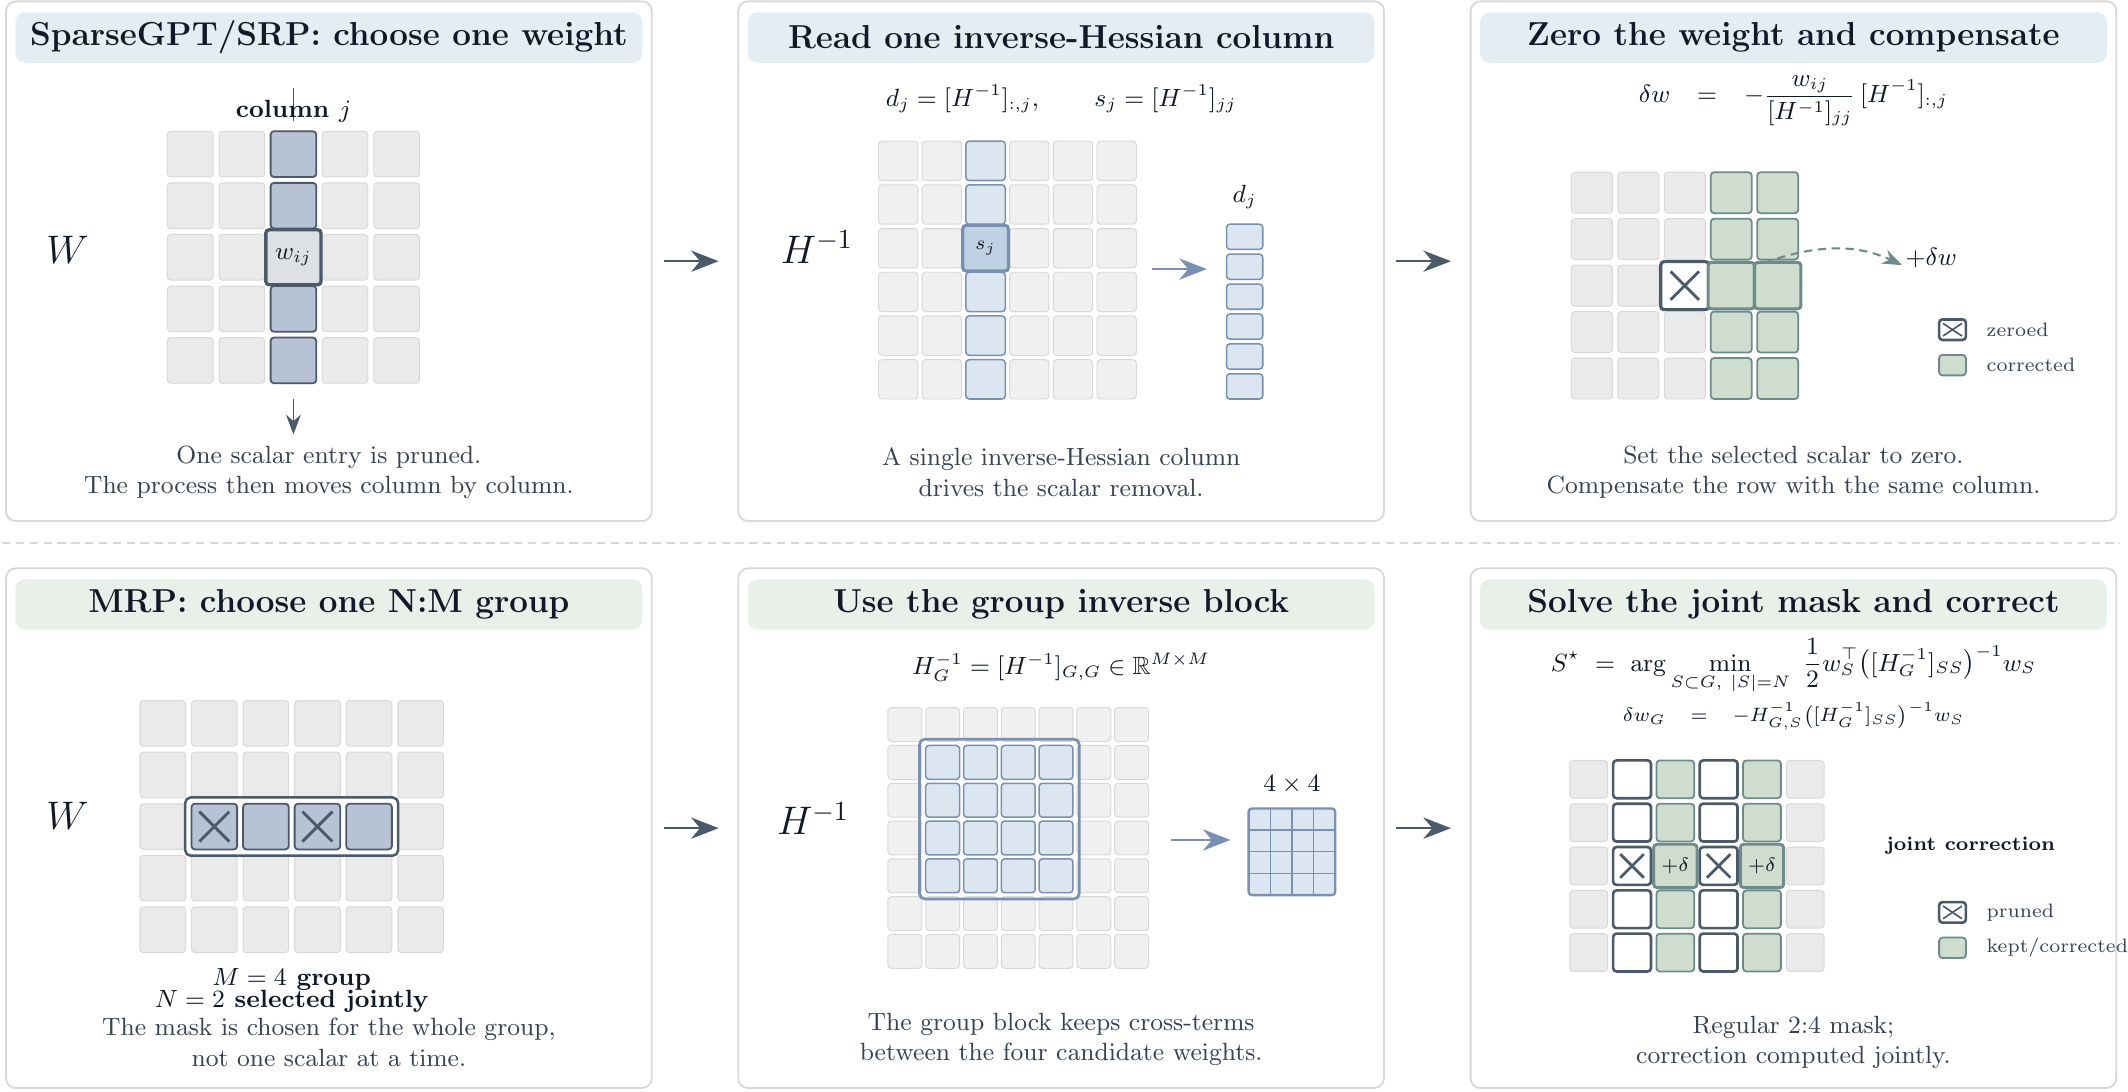
\includegraphics[width=\linewidth]{figures/compression/sparsegpt_mrp_compensation.png}
\caption{Second-order compensation strategies for unstructured and semi-structured pruning. SparseGPT removes one scalar weight per step and compensates using one column of $\hat{H}^{-1}$, while MRP removes an N:M group jointly and uses the block $(\hat{H}^{-1}_{MM})^{-1}$ to model interactions among simultaneously removed weights.}
\label{fig:hessian_compensation}
\end{figure}

\methodsep

\subsubsection{Fisher-Based Post-Training Structured Pruning}

The post-training framework of Kwon et al. \cite{kwon2022fast} applies second-order structured pruning without end-to-end post-pruning weight optimization. Binary masks over attention heads and FFN filters are found by solving
\begin{equation}
	\arg\min_{\mathbf{m}} \mathcal{L}(\mathbf{m})
	\quad \text{s.t.} \quad
	\mathrm{Cost}(\mathbf{m}) \leq C,
\end{equation}
where $\mathrm{Cost}$ is either a FLOPs or measured latency budget. Expanding around the dense mask and applying a diagonal Fisher approximation reduces the search to selecting units with the smallest diagonal Fisher scores subject to the cost constraint. For latency-constrained pruning, a piecewise-linear lookup table replaces the analytical cost model to incorporate real device behavior:
\begin{equation}
	\mathrm{LAT}(\mathbf{m}_{\ell}) =
	\begin{cases}
		0, & \|\mathbf{m}_{\ell}\|_0 = 0, \\
		c, & 0 < \|\mathbf{m}_{\ell}\|_0 \leq T, \\
		a(\|\mathbf{m}_{\ell}\|_0 - T) + c, & \|\mathbf{m}_{\ell}\|_0 > T,
	\end{cases}
\end{equation}
where $c$ is the base latency incurred by any non-empty layer configuration, $T$ is the structural threshold below which latency is approximately constant, and $a$ is the slope capturing how measured latency grows beyond that threshold. All three constants are read from device benchmarks rather than derived analytically.

\methoddetail{Algorithm Overview}
The method proceeds in four steps: (1) diagonal Fisher scores are computed for head and FFN-filter masks on a small calibration set (2K training examples); (2) a FLOPs- or latency-constrained mask search is solved under the diagonal Fisher objective; (3) a block-diagonal Fisher refinement is applied layer by layer to recover interactions ignored by the diagonal approximation; (4) surviving mask values are tuned by layer-wise linear least-squares reconstruction. Because only mask values are updated, the method avoids end-to-end weight retraining. The paper reports pruning times of 39 seconds on GLUE and 135 seconds on SQuAD, compared to 33 hours for CoFi on MNLI.

\methodsep

\subsubsection{Inference-Aware Structured Second-Order Pruning (ZipLM)}

ZipLM \cite{kurtic2023ziplm} applies an OBS-style reconstruction objective to executable Transformer structures rather than scalar weights. For a candidate structure $S$ with column mask $\mathbf{M}_S$, the removal score is
\begin{equation}
	\arg\min_S
	\sum_{i=1}^{d_{\text{row}}}
	\mathbf{W}_{i,\mathbf{M}_S}
	\left(\left(\mathbf{H}^{-1}\right)_{\mathbf{M}_S,\mathbf{M}_S}\right)^{-1}
	\mathbf{W}_{i,\mathbf{M}_S}^{T},
\end{equation}
where $d_{\text{row}}$ is the output dimension of the weight matrix and the sum aggregates the reconstruction cost across all output rows. After removing a structure, the exact compensation and Hessian update are applied through block Gaussian elimination, so that all subsequent saliency scores remain consistent with the already-pruned state.

\methoddetail{Inference-Aware Search}
ZipLM adds a device-level objective on top of the local second-order scoring. It benchmarks attention and FFN configurations on the target hardware and stores measured runtimes in a lookup table. The global search then minimizes layer-wise structural sensitivity subject to a real speed constraint $\sum_\ell \tau_{\ell,s_\ell} \leq T_{\text{target}}$.

\methoddetail{Algorithm Overview}
ZipLM follows an iterative pruning-and-recovery regime in the sense of Section~\ref{subsec:iterative_pruning}: pruning steps are interleaved with fine-tuning rounds rather than applied all at once. It operates in two phases (see Figure~\ref{fig:ziplm_pipeline}). In the global phase, attention-head and FFN configurations are benchmarked on the target environment and a layer-wise sparsity profile satisfying the speedup requirement is selected. In the local phase, each selected layer is compressed by iteratively scoring candidate structures with the structured saliency metric, applying the optimal weight compensation, and updating the inverse Hessian by block Gaussian elimination. Recovery follows a gradual prune-and-fine-tune schedule with combined task, logit, and token-level distillation losses, at a cost of 8--10 fine-tuning epochs per pruning step.

\begin{figure}[H]
	\centering
	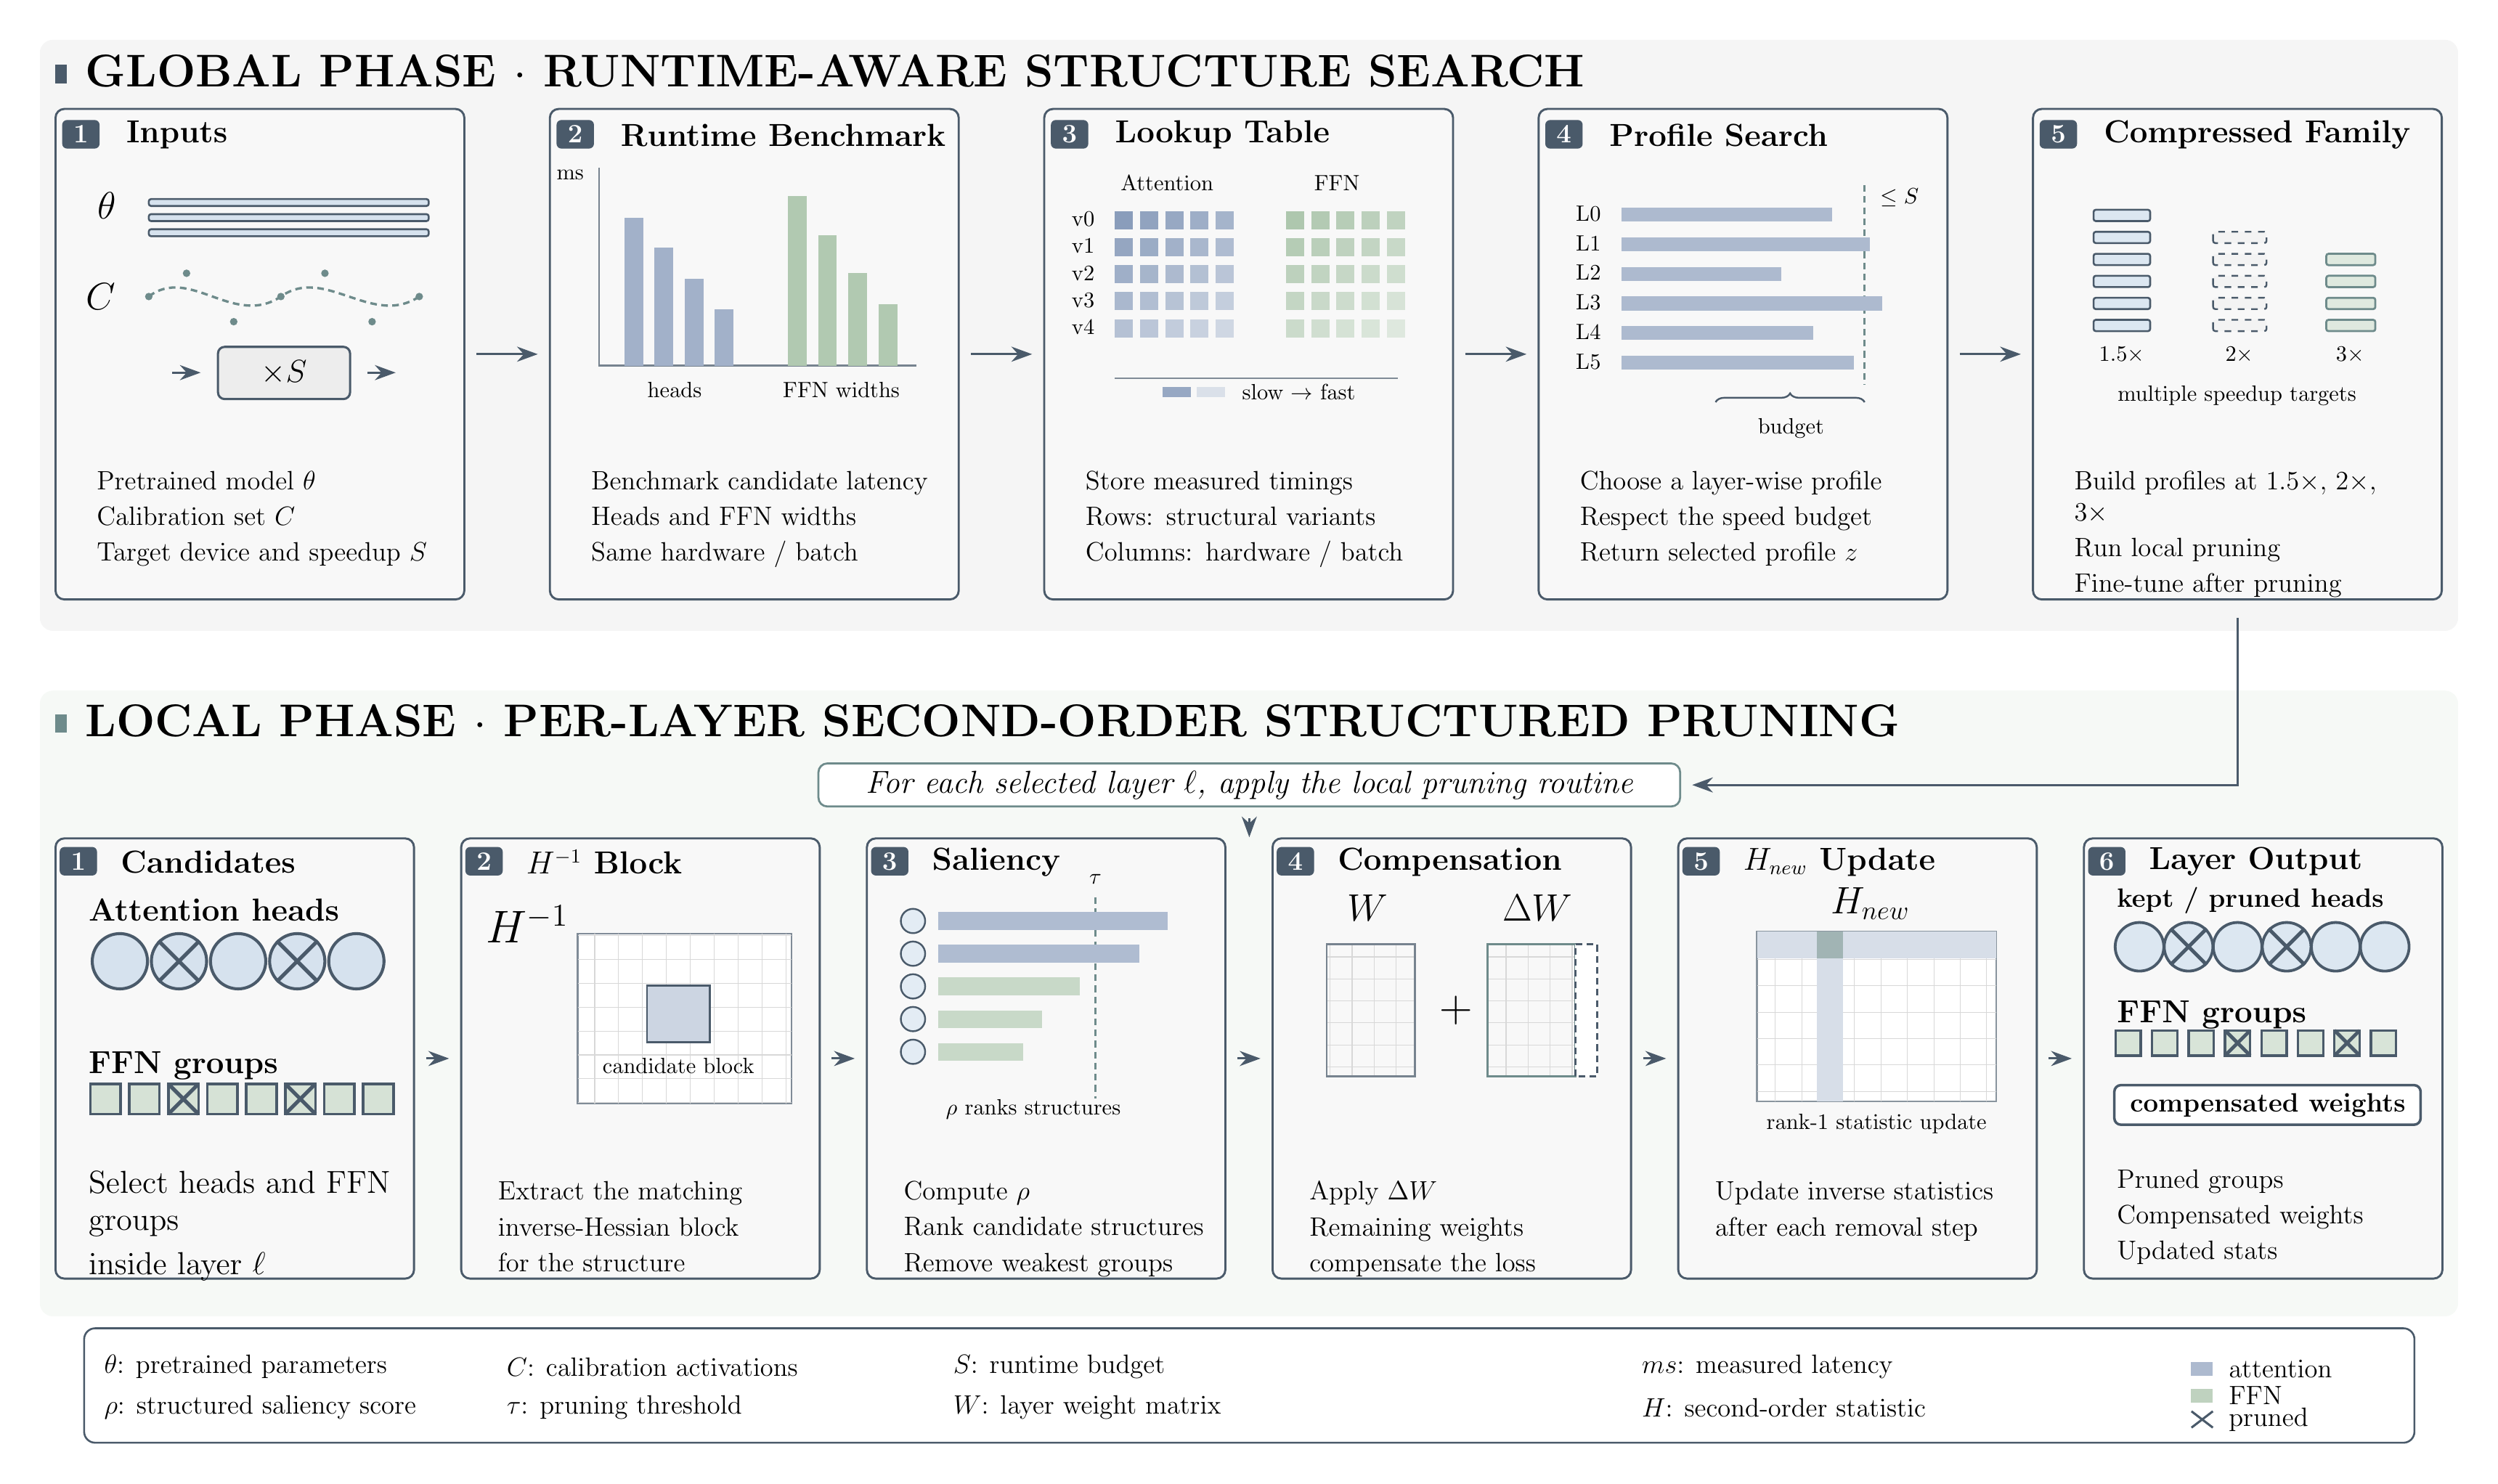
\includegraphics[width=0.96\textwidth]{figures/compression/ziplm_diagram.png}
	\caption{ZipLM pipeline. The global phase benchmarks attention-head and FFN configurations and searches for layer-wise sparsity profiles satisfying the required speedup. The local phase applies second-order structured pruning through inverse-Hessian scoring, compensation updates, and iterative Hessian refinement.}
	\label{fig:ziplm_pipeline}
\end{figure}

Second-order methods reduce local reconstruction error, but they do not fully resolve the allocation problem across the whole model. A method may know how to remove a head or channel with limited local damage and still not know how many heads or FFN channels should remain in each layer under a global budget. This is the point at which search-based methods become relevant.

\subsection{Search-Based Methods}

Search-based methods operate over complete sparsity configurations rather than applying a single closed-form ranking rule to individual units. This is especially relevant when the quality of a pruning decision depends on how several removals interact across layers.

\subsubsection{Constrained Evolutionary Frameworks}
\label{subsec:evopress_pruning}

\paragraph{EvoPress.}
EvoPress \cite{evopress2024} searches over discrete layer-wise compression profiles instead of assigning a single saliency score per layer. A candidate is a configuration $\mathbf{C} = \{c_1,\dots,c_L\}$ where $c_\ell \in \mathcal{S}_\ell$ is the compression level for layer $\ell$. Budget is preserved by level-switch mutation: one layer becomes more compressed only if another becomes less compressed, keeping the global average sparsity $S_{\text{glob}}$ fixed. Mutations are deliberately local, with most offspring differing from the parent by only one or two switches.

Selection proceeds in multiple rounds with increasing token budgets and decreasing survivor counts:
\begin{equation}
	\mathcal{P}^{(r+1)} =
	\operatorname{Top}_{n_{r+1}}
	\left(
	\left\{
	\mathcal{F}_{T_r}(C) \mid C \in \mathcal{P}^{(r)}
	\right\}
	\right),
	\qquad
	T_1<T_2<\cdots,\;
	n_1>n_2>\cdots,
\end{equation}
where the fitness signal is KL divergence to the reference model. This progressive evaluation scheme is what makes EvoPress practically efficient: early rounds use few tokens to discard poor candidates quickly, reserving the full calibration budget for finalists. The method converges in approximately 5--6 GPU hours for a standard Llama-2-7B sparsity search.

Figure~\ref{fig:evolutionary_pruning_flow} summarizes this search loop. The important point is that the algorithm evaluates complete compression profiles, selects promising candidates with increasing evaluation budgets, and mutates the retained profile while preserving the global compression constraint.

\begin{figure}[H]
\centering
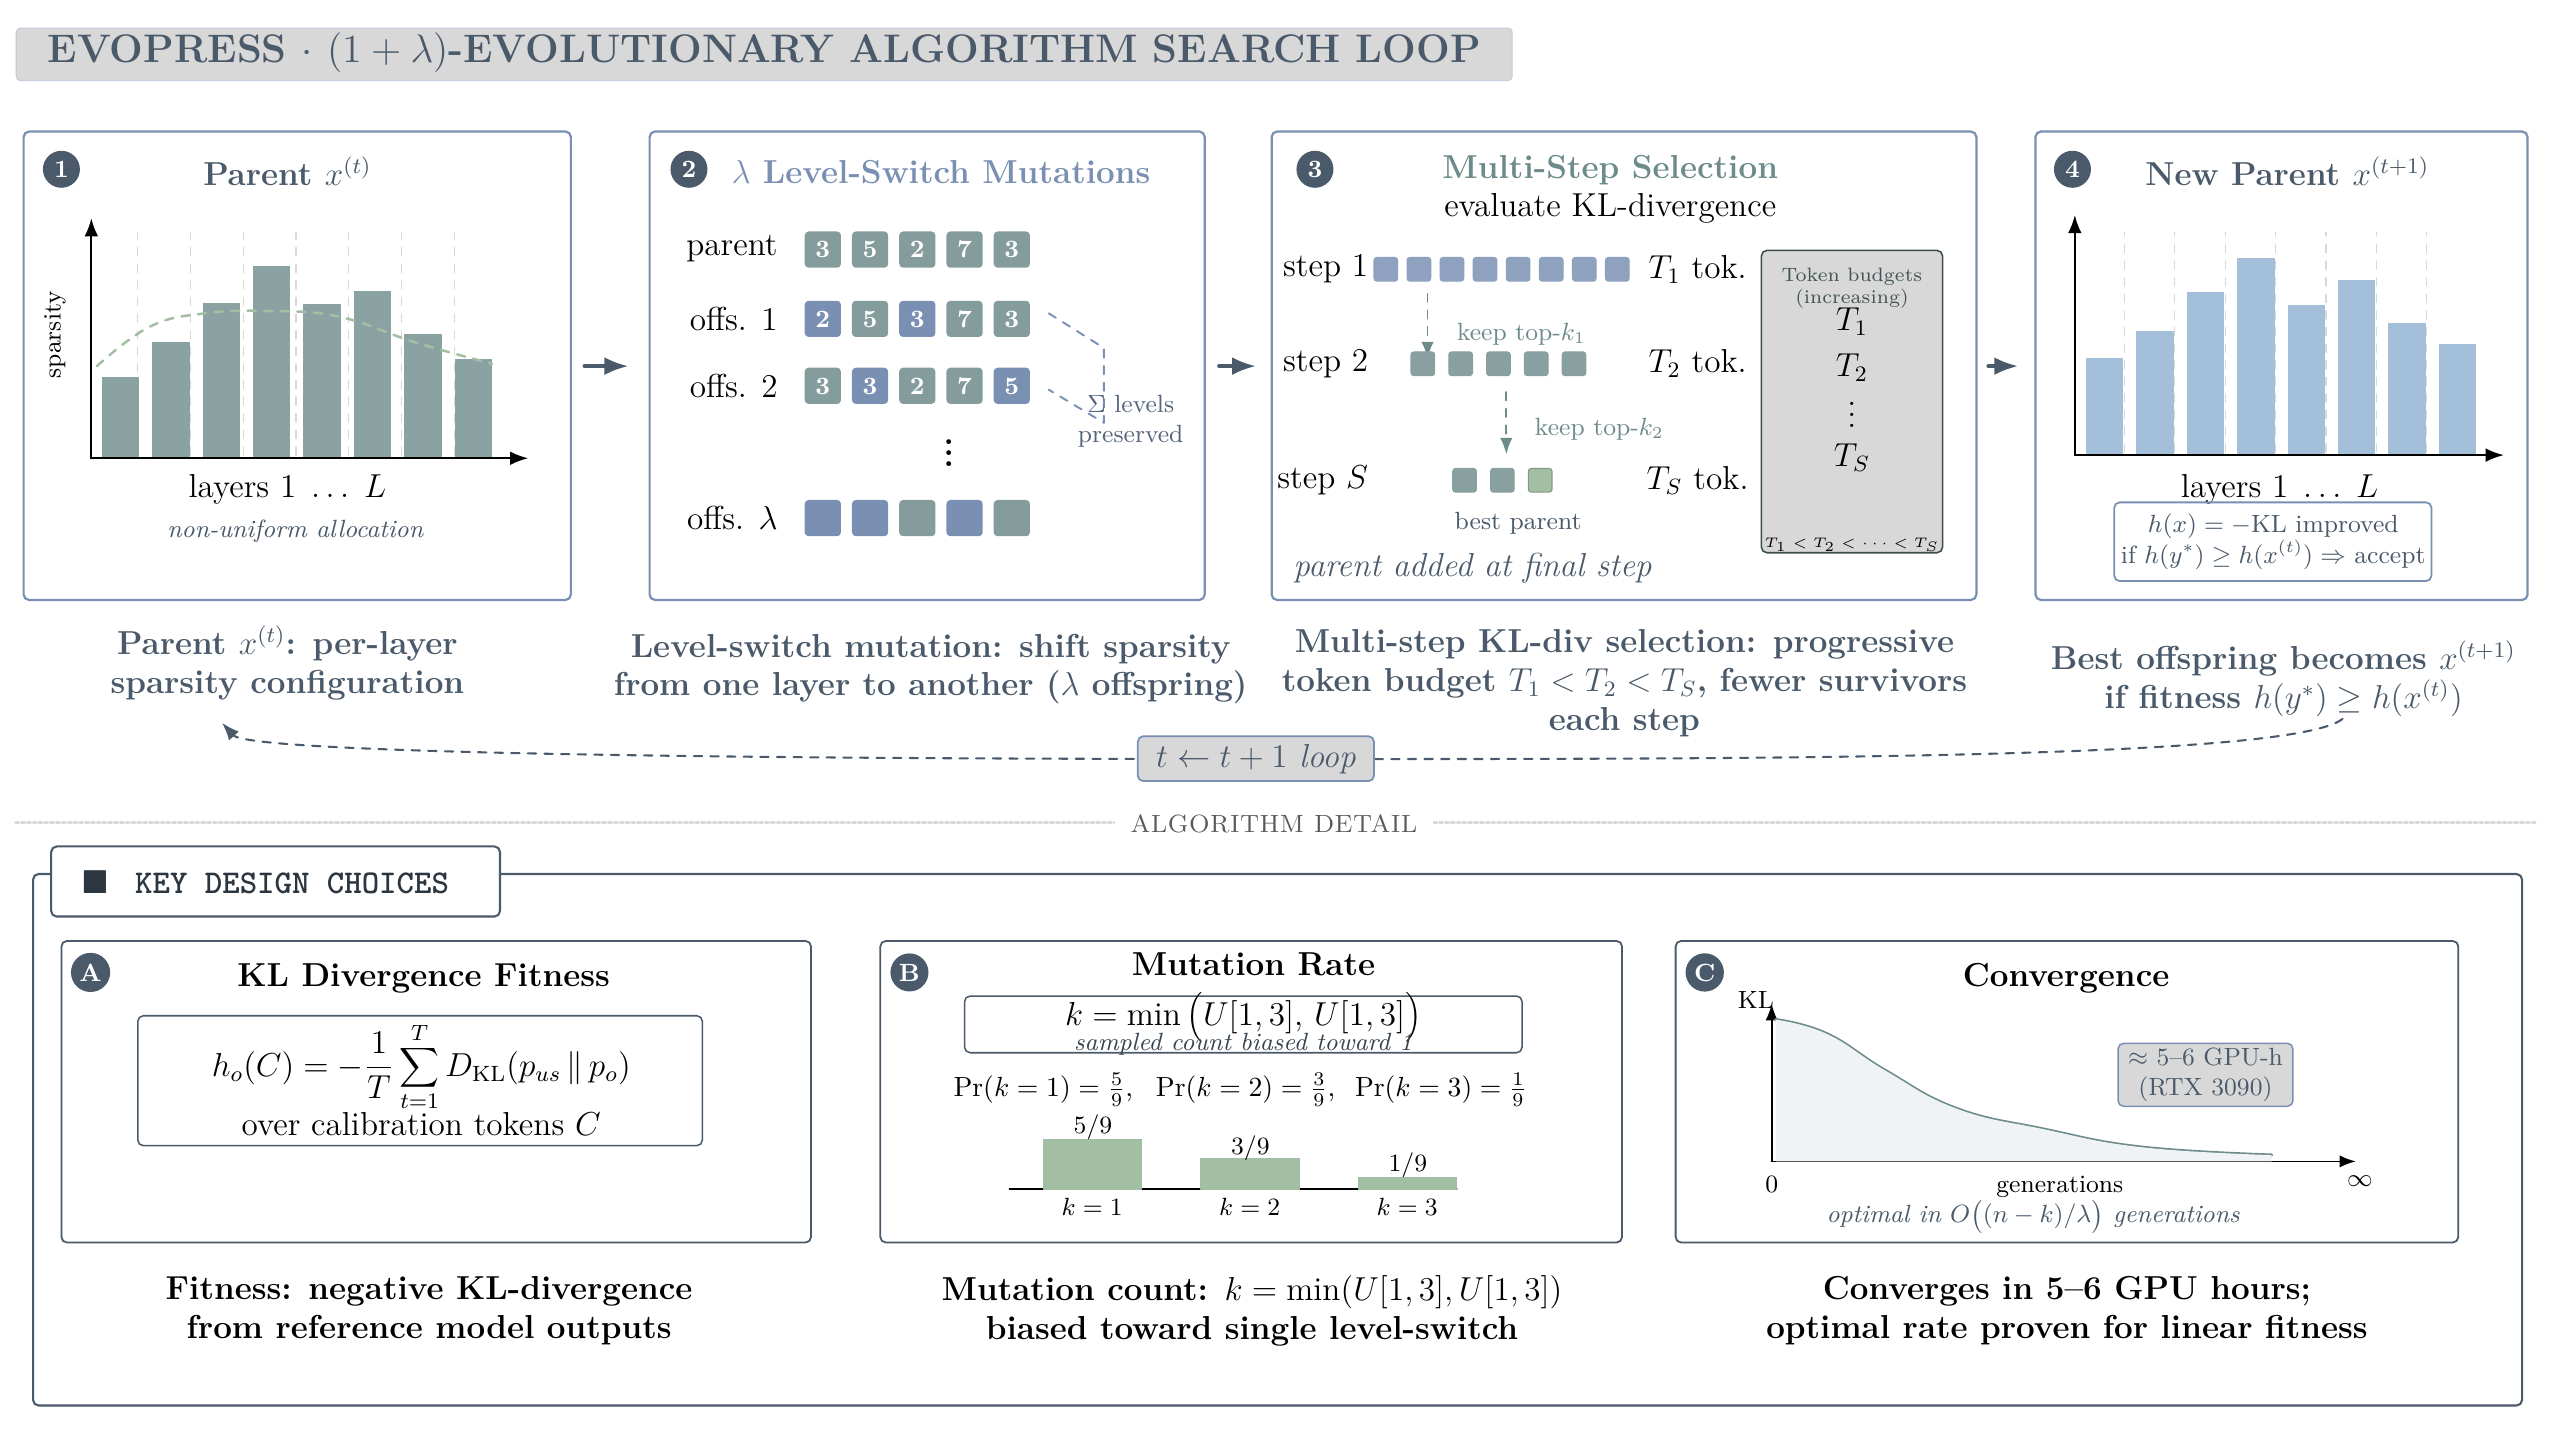
\includegraphics[width=0.94\linewidth,height=0.50\textheight,keepaspectratio]{figures/compression/evopress_search_loop.png}
\caption{EvoPress $(1+\lambda)$ evolutionary search loop for dynamic LLM compression \citep{evopress2024}. The method applies budget-preserving level-switch mutation and progressively evaluates candidates with larger calibration budgets.}
\label{fig:evolutionary_pruning_flow}
\end{figure}
\FloatBarrier

\methodsep

\paragraph{DarwinLM.}
DarwinLM \cite{darwinlm2025} extends evolutionary search to \emph{structured} pruning by unifying OBS-style second-order pruning with a training-aware offspring selection strategy. It differs from EvoPress on three axes: structured granularity (heads and FFN channels), front-loaded Hessian computation stored in a sparsity-level database (SLD), and fitness measured after a short lightweight finetune rather than from the one-shot pruned model.

\methoddetail{Sparsity Level Database}
For each module, DarwinLM solves the structured OBS problem at $N_l$ equally-spaced sparsity levels and stores the pruned-and-compensated weights. The optimal structured mask and compensation are:
\begin{align}
	M^* &= \arg\min_{M}\sum_{i=1}^{d_{\mathrm{row}}}
		\mathbf{W}_{i,M}\bigl(\hat{H}^{-1}_{MM}\bigr)^{-1}\mathbf{W}_{i,M}^\top, \\
	\delta^* &= -\mathbf{W}_{:,M}\bigl(\hat{H}^{-1}_{MM}\bigr)^{-1}\hat{H}^{-1}_{M,:},
\end{align}
where $d_{\mathrm{row}}$ is the output dimension of the module weight matrix, $M$ indexes the pruned columns, and $\hat{H}$ is the empirical Hessian computed from calibration activations. During search, candidate models are assembled by looking up stored entries, avoiding any Hessian recomputation.

\methoddetail{Training-Aware Selection}
Each candidate receives a short lightweight finetune before evaluation:
\begin{equation}
	\mathcal{F}(C_k) = D_{\mathrm{KL}}\!\bigl(\hat{M}\,\|\,\operatorname{finetune}(C_k,\, T_f)\bigr),
\end{equation}
where $\hat{M}$ is the output distribution of the dense reference model and $T_f$ is the fine-tuning token budget. Selection uses three progressive rounds ($T_f \in \{10\text{K}, 50\text{K}, 200\text{K}\}$ tokens) with decreasing survivor counts. The SLD must be computed once per model and sparsity range, making the upfront cost proportional to $L \cdot N_l$ structured OBS operations. DarwinLM compresses Llama-2-7B to 2.7B parameters with higher downstream accuracy than ShearedLlama using $5\times$ fewer post-training tokens (10B vs.\ 50B).

\methoddetail{Algorithm Overview}
DarwinLM sits between a post-training and an iterative regime: the SLD is built offline without end-to-end training, but each search candidate receives a lightweight fine-tune before fitness evaluation. In the offline phase, the SLD is built: for each module and each of $N_l$ sparsity levels, the structured OBS problem is solved and the pruned-and-compensated weights are stored, so that any candidate configuration can be assembled by table lookup rather than recomputation. In the search phase, candidate models are stitched together by selecting one SLD entry per module, then evaluated through that lightweight finetune. Mutation follows the same budget-preserving logic as EvoPress, swapping one module's sparsity level up only if another's is swapped down. Selection proceeds over three rounds with token budgets of 10K, 50K, and 200K and shrinking survivor counts, so weaker candidates are eliminated cheaply before the full evaluation budget is spent. The upfront SLD cost is proportional to $L \cdot N_l$ structured OBS operations and is paid once per model.

Figure~\ref{fig:darwinlm_pruning_flow} shows the corresponding DarwinLM workflow. Compared with EvoPress, the key visual distinction is the front-loaded sparsity-level database: candidate models are assembled from stored structured-pruning choices, then filtered through training-aware selection.

\begin{figure}[H]
\centering
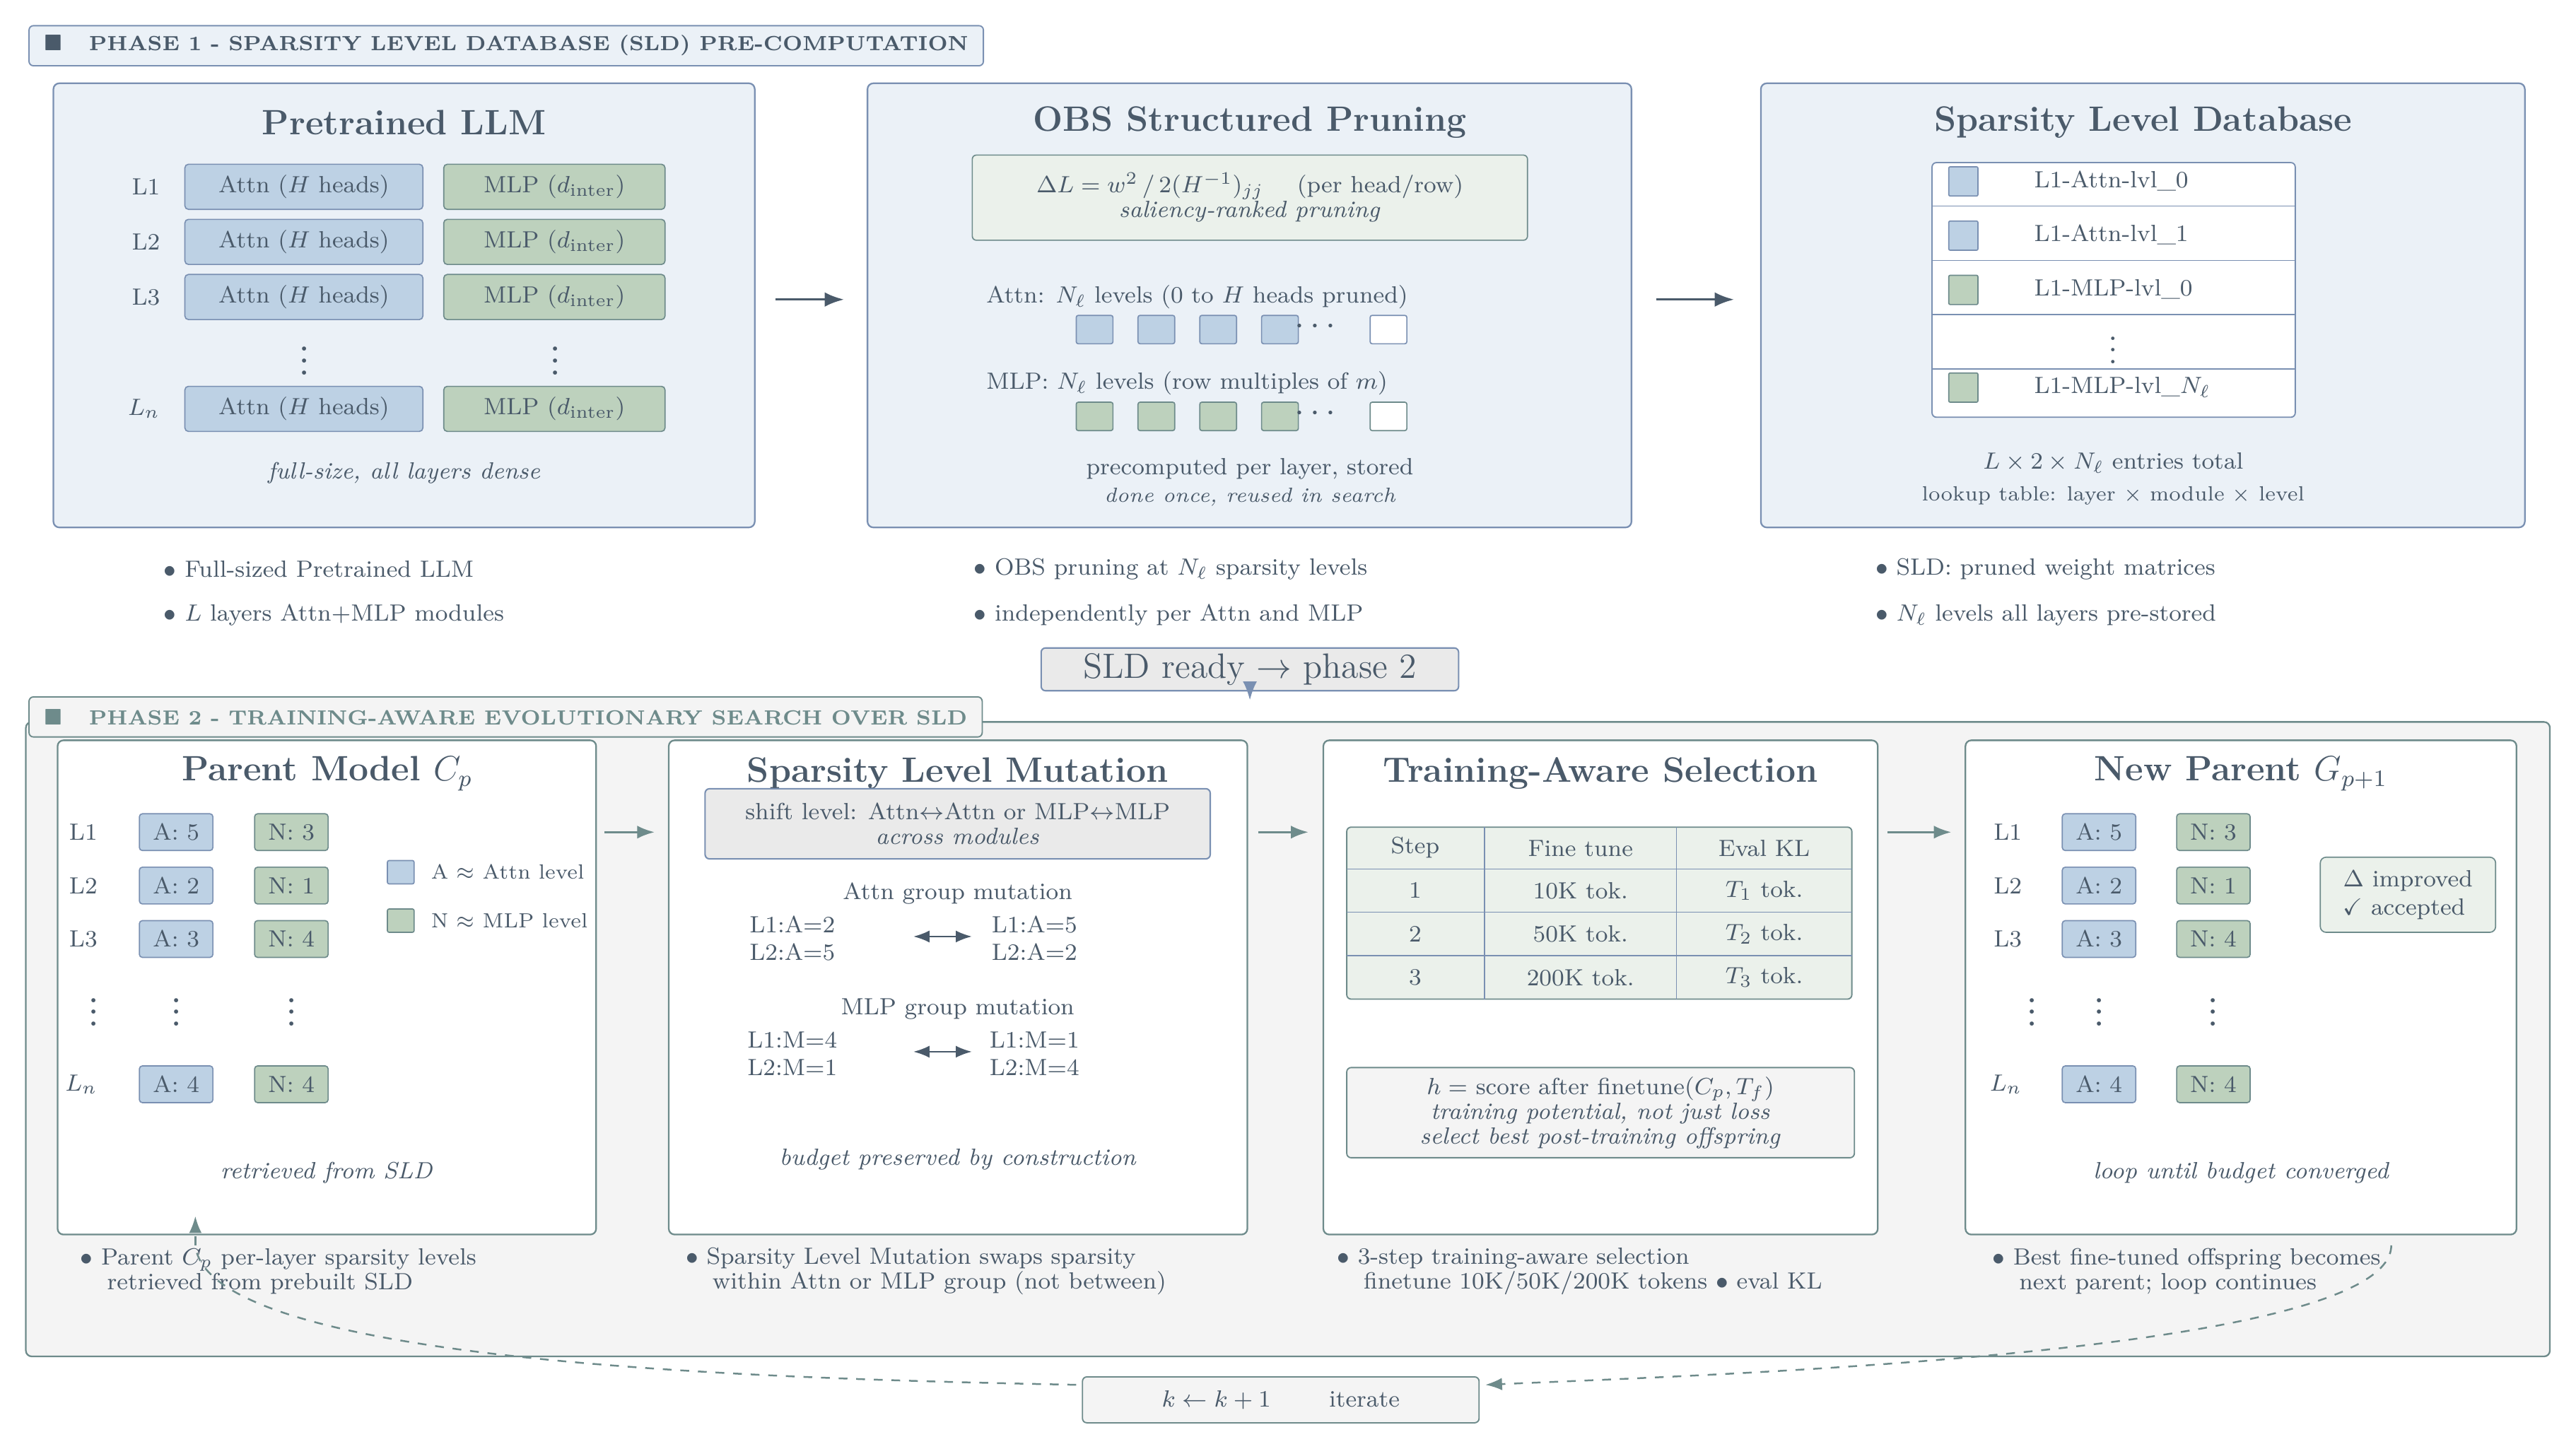
\includegraphics[width=0.94\linewidth,height=0.50\textheight,keepaspectratio]{figures/compression/darwinlm_search_loop.png}
\caption{DarwinLM search loop \citep{darwinlm2025}. The method first builds a sparsity-level database with OBS-style structured pruning, then performs training-aware evolutionary selection over stitched candidate models.}
\label{fig:darwinlm_pruning_flow}
\end{figure}

\FloatBarrier

Table~\ref{tab:preparation_cost_profile} compares the practical preparation cost of the reviewed families. This table is included separately from the empirical results because a method can report strong accuracy while still requiring a substantially different calibration, recovery, benchmarking, or search budget.

\begin{table}[H]
	\centering
	\caption{Preparation cost and evaluation requirements of representative pruning methods. The table separates low-cost post-training scoring, training-dependent structured pruning, curvature-based reconstruction, and population-based search.}
	\label{tab:preparation_cost_profile}
	\begin{tabularx}{\textwidth}{@{}>{\raggedright\arraybackslash}p{2.6cm}LL@{}}
		\toprule
		\textbf{Method} & \textbf{Dominant preprocessing cost} & \textbf{Additional requirement} \\ \midrule
		Magnitude & Linear scan $O(|W|)$ & None \\
		Wanda & Activation collection and linear scoring & Small calibration set ($\approx$128 samples) \\
		CoFi & Multi-epoch joint mask and weight optimization & Task-specific teacher; $\approx$33 h for MNLI \\
		LLM-Pruner & Forward/backward scoring over dependency groups & LoRA recovery ($\approx$2.5 h on RTX 4090) \\
		SparseGPT & Block-wise Hessian estimation and reconstruction & Calibration Hessian \\
		MRP & Group-wise mask search and compensation & Block curvature updates for N:M groups \\
		Fast PTPF & Diagonal or block Fisher estimation with mask tuning & Calibration set; optional latency lookup table \\
		ZipLM & Layer-wise Hessian updates and runtime-table search & Calibration set plus hardware benchmarking pass \\
		EvoPress / DarwinLM & Population search over compression profiles & 1--6 GPU-hours; SLD pre-computation for DarwinLM \\ \bottomrule
	\end{tabularx}
\end{table}

After the main method families have been described, the next step is to compare what they actually report. The empirical results below are therefore organized by pruning regime rather than by derivation, because perplexity, task accuracy, speedup, and recovery cost are not interchangeable measurements.

\subsection{Empirical Comparison}
\label{subsec:empirical_comparison}

The empirical evidence is organized by pruning regime. This avoids treating incompatible measurements as if they were directly comparable: unstructured and N:M methods mainly report perplexity under weight sparsity, structured methods report task accuracy or speedup after architectural removal, and search-based methods report the quality of full pruning configurations under budget constraints.

\subsubsection{Unstructured and Semi-Structured Results}

Table~\ref{tab:unsupported_comparison} keeps representative low, medium, and large model settings rather than listing every available row. The unstructured rows compare magnitude pruning, SparseGPT, and Wanda at 50\% sparsity, while the 2:4 rows show the semi-structured regime that motivates group-aware compensation such as MRP.

\begin{table}[H]
	\centering
	\caption{Representative unstructured and semi-structured pruning results on WikiText perplexity. PPL denotes perplexity; lower is better.}
	\label{tab:unsupported_comparison}
	\begin{tabular}{@{}llcccc@{}}
		\toprule
		\textbf{Model} & \textbf{Setting} & \textbf{Dense PPL} & \textbf{Magnitude PPL} & \textbf{SparseGPT PPL} & \textbf{Wanda PPL} \\
		\midrule
		LLaMA-7B  & 50\% unstructured & 5.68 & 17.29 & 7.22 & 7.26 \\
		LLaMA-30B & 50\% unstructured & 4.77 & 7.54  & 5.31 & 5.24 \\
		LLaMA-65B & 50\% unstructured & 3.56 & 5.90  & 4.57 & 4.57 \\
		\midrule
		OPT-13B   & 50\% unstructured & 10.13 & $1.2{\times}10^4$ & 11.17 & -- \\
		OPT-175B  & 50\% unstructured & 8.35  & $4.3{\times}10^4$ & 8.21  & -- \\
		\midrule
		OPT-13B   & 2:4 semi-structured & 10.13 & -- & 12.96 & -- \\
		OPT-66B   & 2:4 semi-structured & 9.34  & -- & 10.09 & -- \\
		OPT-175B  & 2:4 semi-structured & 8.35  & -- & 8.74  & -- \\
		\bottomrule
	\end{tabular}
\end{table}

The table shows two separate points. First, pure magnitude pruning can fail badly at 50\% sparsity, while activation-aware and second-order methods preserve perplexity much more effectively. Second, semi-structured 2:4 pruning remains more constrained than unconstrained unstructured pruning, so the compensation mechanism must respect the local group structure.

\subsubsection{Structured Pruning Results}

Table~\ref{tab:structured_summary} summarizes representative structured-pruning results without listing every benchmark. The rows are selected to show low, medium, and high compression or speedup regimes where available, while keeping the evaluation suite explicit: CoFi is reported on GLUE tasks and SQuADv1, Fast PTPF reports GLUE/SQuAD results, and ZipLM reports GLUE-style classification tasks as well as SQuADv1.

\begin{table}[H]
	\centering
	\caption{Representative structured Transformer pruning results across recovery regimes. GLUE denotes the General Language Understanding Evaluation benchmark, SQuADv1 denotes Stanford Question Answering Dataset version 1.1, acc. denotes accuracy, and F1 denotes question-answering F1 score.}
	\label{tab:structured_summary}
	\begin{tabular}{@{}llp{4.4cm}p{4.7cm}@{}}
		\toprule
		\textbf{Method} & \textbf{Model} & \textbf{Setting} & \textbf{Key result} \\
		\midrule
		LLM-Pruner \cite{ma2023llmpruner}
		  & LLaMA-7B & 20\% prune ratio & 98.6\% zero-shot accuracy retention after LoRA recovery \\
		  & LLaMA-7B & 50\% prune ratio & 83.6\% zero-shot accuracy retention after LoRA recovery \\
		\midrule
		CoFi \cite{xia2022structured}
		  & BERT Base & GLUE/MNLI, $\approx 12{\times}$ speedup & 80.6 acc. versus 78.8 for TinyBERT$_4$ at similar speedup \\
		  & BERT Base & SQuADv1, $\approx 8.7{\times}$ speedup & 82.6 F1, matching TinyBERT$_4$ at comparable speedup \\
		\midrule
		Fast PTPF \cite{kwon2022fast}
		  & BERT Base & GLUE and SQuADv1, FLOPs-constrained pruning & 60--70\% FLOPs with $\leq 1\%$ accuracy/F1 drop \\
		  & BERT Base & GLUE and SQuADv1, latency-constrained pruning on V100 & $1.34{\times}$--$1.47{\times}$ geometric-mean speedup depending on batch size \\
		\midrule
		ZipLM \cite{kurtic2023ziplm}
		  & BERT Base & GLUE/QNLI and MNLI, $2{\times}$ speedup & 91.4 / 84.8 acc.; essentially dense-level performance \\
		  & BERT Base & GLUE/QNLI and MNLI, $10{\times}$ speedup & 88.6 / 82.7 acc.; approximately 5M parameters \\
		  & BERT Large & SQuADv1, $10{\times}$ speedup & 89.1 F1 with 20.9M parameters \\
		\bottomrule
	\end{tabular}
\end{table}

The structured results are closer to deployment because they remove executable units, but they are also harder to compare directly. GLUE classification tasks and SQuADv1 question answering measure different behavior, and the recovery protocols also differ: CoFi uses task-specific training, LLM-Pruner depends on LoRA recovery, Fast PTPF is largely post-training, and ZipLM adds device-specific runtime profiling.

\subsubsection{Evolutionary and Search-Based Results}

Table~\ref{tab:search_summary} keeps representative search-based results and includes both EvoPress and DarwinLM. EvoPress illustrates configuration search for depth pruning and sparsity allocation, while DarwinLM shows structured evolutionary pruning with training-aware offspring selection.

\begin{table}[H]
	\centering
	\caption{Representative search-based pruning results. Wiki2 and C4 are perplexity values where lower is better; task average is accuracy where higher is better.}
	\label{tab:search_summary}
	\begin{tabular}{@{}llllccc@{}}
		\toprule
		\textbf{Setting} & \textbf{Model} & \textbf{Budget} & \textbf{Method} & \textbf{Wiki2$\downarrow$} & \textbf{C4$\downarrow$} & \textbf{Task Avg.$\uparrow$} \\
		\midrule
		Depth pruning
		  & Mistral-7B & 25\% & EvoPress & \textbf{8.66} & \textbf{12.04} & -- \\
		  & Mistral-7B & 25\% & ShortGPT & 43.26 & 40.16 & -- \\
		  & Mistral-7B & 25\% & Shortened LLaMA & 14.94 & 19.30 & -- \\
		\midrule
		Depth pruning
		  & Llama-2-7B & 37.5\% & EvoPress & \textbf{17.98} & \textbf{18.91} & -- \\
		  & Llama-2-7B & 37.5\% & ShortGPT & 70.94 & 63.51 & -- \\
		  & Llama-2-7B & 37.5\% & Shortened LLaMA & 35.37 & 26.07 & -- \\
		\midrule
		Unstructured allocation
		  & Mistral-7B & 70\% & EvoPress & \textbf{14.42} & \textbf{16.46} & \textbf{53.8} \\
		  & Mistral-7B & 70\% & OWL & 17.22 & 21.66 & 51.9 \\
		  & Mistral-7B & 70\% & Uniform & 23.08 & 30.03 & 49.9 \\
		\midrule
		Structured search
		  & Llama-2-7B & 2.7B model & DarwinLM & -- & -- & 62.8 after 10B-token post-training \\
		  & Llama-2-7B & 2.7B model & ShearedLLaMA & -- & -- & 62.6 after 50B-token post-training \\
		\bottomrule
	\end{tabular}
\end{table}

The search results support the same conclusion from two directions. EvoPress improves over local or heuristic allocation when multiple removals interact, and DarwinLM shows that training-aware evolutionary selection can produce stronger structured models with less post-training data than a fixed pruning baseline.

\subsubsection{Cross-Regime Synthesis}

Table~\ref{tab:pruning_empirical_summary} aggregates the evidence at a higher level. It is not meant to replace the detailed result tables above; it summarizes what each regime establishes for the design of a pruning-search method.

\begin{table}[H]
	\centering
	\caption{Aggregated interpretation of the empirical pruning evidence by regime.}
	\label{tab:pruning_empirical_summary}
	\begin{tabularx}{\textwidth}{@{}>{\raggedright\arraybackslash}p{2.5cm}>{\raggedright\arraybackslash}p{3.0cm}LL@{}}
		\toprule
		\textbf{Regime} & \textbf{Representative setting} & \textbf{Selected evidence} & \textbf{Reading} \\
		\midrule
		Weight-level unstructured
		& LLaMA-7B, 50\% sparsity
		& Dense PPL 5.68; magnitude 17.29; SparseGPT 7.22; Wanda 7.26.
		& Better saliency preserves perplexity, but the resulting pattern remains unstructured and does not guarantee dense-kernel speedup. \\
		\addlinespace
		Semi-structured N:M
		& OPT-13B, 2:4 sparsity
		& Dense PPL 10.13; SparseGPT-style compensation gives 12.96 under the 2:4 constraint.
		& N:M sparsity needs group-aware compensation, which motivates MRP-style joint treatment of simultaneously removed weights. \\
		\addlinespace
		Structured LLM pruning
		& LLM-Pruner on LLaMA-7B
		& 20\% prune ratio retains 98.6\% zero-shot accuracy after LoRA recovery; 50\% retains 83.6\%.
		& Dependency-aware pruning keeps the model executable, but the final quality depends strongly on recovery. \\
		\addlinespace
		Structured encoder pruning
		& CoFi, Fast PTPF, and ZipLM on BERT
		& CoFi reaches 80.6 MNLI acc. near $12{\times}$ speedup; Fast PTPF keeps 60--70\% FLOPs with $\leq$1\% drop; ZipLM reaches 88.6/82.7 QNLI/MNLI acc. at $10{\times}$ speedup.
		& Structured pruning can produce executable acceleration, but the protocols differ in training cost, hardware profiling, and recovery budget. \\
		\addlinespace
		Search-based pruning
		& EvoPress and DarwinLM
		& EvoPress improves depth-pruning and sparsity-allocation baselines; DarwinLM reports 62.8 average accuracy after 10B-token post-training versus 62.6 for ShearedLLaMA after 50B tokens.
		& Configuration search addresses global allocation, while training-aware selection improves structured candidates beyond one-shot scoring. \\
		\bottomrule
	\end{tabularx}
\end{table}

\begingroup
\def\RenderPruningReviewDiscussion{}
% ============================================================
%  Drop-in discussion sections, compile inside your main .tex
%  Requires: amsmath, booktabs, enumitem, hyperref, algorithm,
%            algpseudocode, multirow, tabularx, array, xcolor
% ============================================================

% =============================================================
\ifdefined\RenderPruningReviewDiscussion
\section{Discussion}
\label{sec:discussion}
% =============================================================

The distinction between the two questions has been separated between Chapters~\ref{chap:related_work_pruning_unstructured} and~\ref{chap:related_work_pruning_structured} and in the empirical comparison, Section~\ref{subsec:empirical_comparison}. One question is: for a single unit that is potentially removable, what criterion should be used to rank the units? Here, different magnitude-based, gradient-based, and curvature-based criteria offer varying estimates. The second question is: how is the overall budget of pruning shared among the units in the model? Here, the approaches tend to diverge more substantially, and much of the outstanding debate in the literature is focused on the latter. It will be discussed here, then the empirical data.

\subsection{Local Scoring Versus Global Allocation}
\label{subsec:local_vs_global}

The methods reviewed in this chapter differ in implementation, pruning unit, and recovery cost, but they can all be related to the same underlying objective:
\begin{equation}
  \min_{\mathcal{M} \in \mathcal{F}}\; \Delta\mathcal{L}(\mathcal{M}),
  \label{eq:master}
\end{equation}
where $\mathcal{M}$ denotes a feasible sparsity pattern or structured subnetwork and $\Delta\mathcal{L}$ denotes the loss increase caused by pruning. The difficulty is that $\mathcal{M}$ must satisfy a compression budget while preserving the behaviour of the model.

Another persistent issue with the pruning criteria discussed so far is their evaluation of weights and activations, which can be removed before the final compressed model is fixed. SparseGPT calculates approximate second-order local reconstruction costs of sets of weights \cite{frantar2023sparsegpt}, while Wanda sorts parameters by a product of weight magnitude and input activation norm \cite{sun2023simple}. These methods are successful in finding some locally removable weights but fail to determine the overall distribution of compression under a fixed budget across the layers \cite{hoefler2021sparsity,cheng2024pruningsurvey}. Though one-shot local pruning works well under low compression ratios, high compression rates require more sophisticated iterative and global-allocation-based pruning methods \cite{janusz2025oneshot}. Several of these recent methods implicitly or explicitly address this issue: ZipLM attempts to find explicit local and global correlations between layers, and EvoPress directly searches over the layer-wise compression budgets that minimize the distribution divergence of the output \cite{kurtic2023ziplm,evopress2024}.

\subsection{Limitations of Local Ranking at High Compression}
\label{subsec:inadequacy}

In the analyses above, we can observe one trend across these method families. It appears that local ranking criteria are successful when the compression ratio is relatively small to medium; when the targeted compression ratio becomes higher, the deficiencies of local ranking criteria tend to become apparent \cite{hoefler2021sparsity,sanh2020movement,bai2024sparsellm,janusz2025oneshot}. This pattern is expected from the definition of the pruning problem: local criteria judge removeable units while the ultimate compressed model has not been formed completely.

For Transformer models, structured pruning is naturally expressed as a layer-wise allocation problem over executable units. A pruned Transformer may retain different numbers of attention heads, FFN intermediate dimensions, hidden dimensions, or even complete MHA/FFN modules in different layers \cite{xia2022structured,kurtic2023ziplm,cheng2024pruningsurvey}. Thus, for a model with $L$ layers, $H$ attention heads per layer, and $F$ FFN channels per layer, the retained structure can be represented by an allocation vector
\[
  \mathbf{s} = (h_1, f_1, h_2, f_2, \ldots, h_L, f_L),
\]
subject to a global MAC budget $\Omega$. Recent layer-wise pruning work therefore treats compression as the problem of assigning adaptive sparsity ratios across layers which is just a specific case of non uniform pruning \cite{li2024dsa}.

Local ranking simply assigns each prunable unit a saliency and prunes the lowest ones until the budget is exhausted. it implicitly models global ranking with the assumption that each pruning decision can be made in isolation. EvoPress recognizes this assumption in the domain of depth pruning; block-scoring algorithms use the assumption that error is linear such that each block is thought to contribute equally to the overall compression error \cite{evopress2024}. ZipLM takes the reverse argument, stating that pruning has to capture both within layer local correlations and across layer global correlations \cite{kurtic2023ziplm}.

The compositional structure of the Transformer violates the independence approximation. Each Transformer block comprises the residual-connected attention and feed-forward sublayers and self-attention layers take representations as input which are generated from previous layers \cite{vaswani2017attention}. With regard to pruning, this indicates that any alteration on one layer will bring new input distribution for the following layers. SparseLLM is the first one who precisely identifies the problem by modeling an LLM as a chain of modules, where outputs of a module become the inputs for another, and points out that local layer error reduction only causes non-optimal performance for the global pruning at a high sparsity rate \cite{bai2024sparsellm}.

The same coupling is present for attention and the global budget constraint. Scaled dot-product attention normalizes the query-key score using a softmax, while multi-head attention merges multiple heads which act on the same input layer \cite{vaswani2017attention}. Experimentally, attention heads can have unequal importance, numerous can be dropped, beyond a threshold, attention collapses catastrophically, and different components of the attention function can have differing sensitivity \cite{michel2022not}. In addition, if the MAC budget is fixed, having high capacity in one layer means we must sacrifice capacity elsewhere. Prior works have indicated the necessity of across-layer uneven sparsity under high compression \cite{gale2019state,sanh2020movement,li2024dsa}.

% =============================================================
\section{Empirical Results}
\label{sec:empirical}
% =============================================================

Having argued that allocation is more important than local scoring at high compression, the question is whether the results reflect this. On the whole, they do but only if we treat apples and oranges distinctly. The results on the unstructured model isolate the saliency rule in the absence of weight sparsity and the structured/search based readings bring back the cost of recovery and the budget allocation aspect.

\subsection{Unstructured and Semi-Structured Methods}
\label{subsec:unstructured_results}

The unstructured pruning results allow three clean comparisons across increasing levels of local sophistication: magnitude baseline, Wanda (activation-aware saliency), and SparseGPT (second-order compensation).

The SparseGPT results primarily highlight the instability of pure magnitude pruning at high sparsity. At 50\% sparsity on OPT-13B, magnitude pruning produces a perplexity of $1.2\times10^4$ compared to the dense model's 10.13. This indicates severe representational degradation under weight selection based solely on individual magnitude. SparseGPT reduces the same setting to 11.17, corresponding to a $+1.04$ increase over the dense model.

The comparison between Wanda and SparseGPT on LLaMA models is also instructive. At 50\% sparsity on LLaMA-7B, Wanda achieves 7.26 versus SparseGPT's 7.22, a negligible 0.04 point difference. On LLaMA-13B, Wanda actually outperforms SparseGPT by 0.06 points (6.15 versus 6.21). This apparent paradox reflects two facts. First, the Wanda activation norm $\|x_j\|_2$ is an effective proxy for the weight's contribution to the output, particularly in models with large activation outliers, which LLaMA models exhibit. Second, the calibration set used for Hessian construction in SparseGPT introduces variance that at moderate sparsity levels can offset the theoretical advantage of curvature information. At higher sparsity levels (70\%+), the second-order advantage of SparseGPT becomes more consistent, because local reconstruction errors accumulate and the precise compensation direction matters more.

\subsection{Structured Methods}
\label{subsec:structured_results_discussion}

Both CoFi and ZipLM obtain similar accuracy at similar speedups but employ very different preparation pipeline. CoFi obtains 80.6 on MNLI with about $12\times$ speedups after 20 hours of combined mask and weight optimization, whereas ZipLM gets 81.7 at $35\times$ through scheduled fine-tuning interspersed with structured pruning stages and dedicated hardware benchmarking. Here the accuracies represent the accuracy of the whole pipeline not only the pruning criterion, because the recovery approaches they employ differ greatly and thus the two methods are not directly comparable.

\subsection{Cross-Method Comparison}
\label{subsec:cross_method}

The tables above support two conclusions. At 50\% unstructured sparsity on OPT-13B, magnitude pruning collapses to a perplexity of $1.2\times10^4$ while SparseGPT reaches 11.17 (Table~\ref{tab:unsupported_comparison}), showing that second-order compensation is necessary once individual weight interactions become non-negligible. At 70\% unstructured sparsity on Mistral-7B, EvoPress reaches 14.42 perplexity while uniform allocation reaches 23.08 (Table~\ref{tab:search_summary}), and at 37.5\% depth sparsity on Llama-2-7B, EvoPress gives 17.98 against ShortGPT's 70.94, showing that global allocation search becomes the dominant factor at high compression.

\section{Limitations of the Reviewed Methods}
\label{sec:limitations}

 The observations above suggest genuine differences between the methods. However, most of the disparity observed is can simply be a reflection of how each paper was evaluated. There are three consistent issues which have affected nearly every cross-paper assertion: unequal testing scenarios, disparate recovery budget sizes and sensitivity to a calibration set whose effect is usually not examined.

\subsection{Evaluation Protocol Heterogeneity}
\label{subsec:eval_protocol}

A significant drawback in the pruning literature is the lack of a universal evaluation protocol. Approaches are presented under five, and possibly more, different evaluation schemes. The first reports language model perplexity under fixed nominal sparsity, while the second measures zero-shot task performance accuracy with or without recovery. The third instead reports supervised fine-tuning performance accuracy with or without recovery, whereas the fourth measures actual wall-clock speedup or latency given particular hardware. Finally, the fifth reports FLOPs reduction compared to the dense model.

These five schemes are incommensurable. A method presenting $99\%$ dense accuracy after $2\times$ FLOPs reduction addresses a different evaluation goal compared to another method presenting $1.5\times$ wall-clock speedup at a $<1\%$ accuracy drop. FLOPs is a hardware-agnostic theoretical metric that does not necessarily linearly translate to wall-clock runtime, which depends on memory bandwidth, batch size, and the particular accelerator execution model. Certain sparse execution formats require hardware support, while the simple unstructured masks often do not result in a proportional wall-clock speedup over standard dense kernels.

The fragmentation of evaluation makes it difficult to compare across papers. If a table presents Wanda~\cite{sun2023simple}, CoFi~\cite{xia2022structured}, LLM-Pruner~\cite{ma2023llmpruner}, ZipLM~\cite{kurtic2023ziplm}, and EvoPress~\cite{evopress2024} in the same rows, one implicitly assumes that they all aim to solve the same problem. In reality, each method targets different budgets, recovery schemes, and deployment targets. When summarized without qualification, the methods present a false picture of one single Pareto frontier.

\subsection{Recovery Budget Inconsistency}
\label{subsec:recovery}

Relatedly is the issue of different recovery budgets. It's expected that structured pruning results in a larger loss in accuracy than unstructured pruning for a given sparsity, making the recovery stage particularly important \cite{xu2026lightweight}. The difference in terminology of ``post-training pruning'' versus ``pruning with fine-tuning'' in reality represents a wide range of recovery costs that contribute to reported accuracy. Among the methods in the above literature, Fisher post-training pruning only tunings the masks with zero weight updates and total tuning time about 39 sec. LLM-Pruner tunings using 2.5 hrs of LoRA recovery on 50k examples with rank 8 adapter. ZipLM tunes over 8-10 epochs per pruning steps with the whole model fine-tuning and full distillation. CoFi joint tunes mask and weights in 40 epochs with a task specific teacher model.

An appropriate comparison needs to keep recovery budgets constant. The model of 40 epochs fine-tuning for CoFi should not be compared to LLM-Pruner's 2.5 hrs of LoRA recovery. Given the same budget, the gap would be much smaller. Very few articles performed such fair comparisons, and thus, some accuracy differences we see in the literature should be attributed to the amount of recovery budget.

\subsection{Calibration Set Sensitivity}
\label{subsec:calibration}

All post-training pruning techniques rely on a calibration set in order to compute either saliency scores, Hessian surrogates, or Fisher information matrices. The specific selection of the calibration set results in differences in the resulting pruned model which are usually not explored in a principled way.

For language models, it is a common practice to use 128–2048 examples from a general language corpus like C4 or WikiText. This is a small fraction of the model’s training distribution, and may not be representative of activation statistics used to determine saliency. LLM-Pruner calibrates using 10 short examples, which is dramatically fewer than SparseGPT's 128 examples and may contribute to variance in its Taylor scores, and consequently in its reported zero-shot accuracies across trials. More generally, all methods employing a calibration set make the implicit assumption that a ranking based on calibration examples transfers to the whole evaluation distribution. It has recently been shown that the calibration set is extremely important in post-training pruning, especially for high sparsity rates, and that pruning works better with calibration data that matches the pre-training distribution \cite{ji2025calibration,bandari2024calibration}.{ji2025calibration,bandari2024calibration}.

% =============================================================
\fi
\ifdefined\RenderProposedPruningSearchFramework
\chapter{Proposed Pruning-Search Framework}
\label{sec:design}
\label{chap:proposed_pruning_search_framework}
% =============================================================

\section{Design Philosophy and Motivation}
\label{subsec:design_philosophy}

The design of the proposed framework follows directly from the gaps identified in Sections~\ref{sec:discussion}--\ref{sec:limitations}. The central premise is that structured pruning at moderate-to-high compression rates is a combinatorial optimisation problem over architectural configurations. The main methodological deficiency in the reviewed methods lies in global allocation strategy rather than in local saliency estimation alone. The pruning-search paper addresses this point explicitly by treating head retention, FFN width, and active depth as a joint discrete decision and by organising the search around feasibility, representation fidelity, and diversity preservation.

Three design principles follow from this premise.
z
\medskip\noindent\textbf{Principle 1: The configuration is the primary optimisation object.} The framework treats the allocation vector $\mathcal{C} = (\mathbf{h}, \mathbf{n})$ as the optimisation variable. Every operation is defined on complete configurations rather than on per-unit scores. This allows direct evaluation of the joint effect of all removals and keeps the budget constraint explicit throughout the search.

\medskip\noindent\textbf{Principle 2: The feasible set is explicitly enforced.} Rather than soft-penalising infeasible configurations, the framework enforces the MAC constraint and minimum active-depth requirement through a repair projection that maps every mutated configuration back into $\mathcal{F}$ before fitness evaluation. This guarantees that every evaluation corresponds to a deployable architecture.

\medskip\noindent\textbf{Principle 3: Diversity is as important as fitness.} Because the configuration space contains many local optima that are structurally distant from each other, a search that maximises raw fitness without diversity control will converge to one architectural type and miss better solutions elsewhere. The framework therefore maintains diversity explicitly through shared-fitness selection, MAP-Elites archiving, and Pareto preservation.

\section{Configuration Space Formalisation}
\label{subsec:config_space}

The pruning-search paper formalises the search variable as a joint head-and-neuron configuration. For a Transformer with $L$ layers and $H$ heads per layer, the candidate is
\begin{equation}
  \mathcal{C} = (\mathbf{h}, \mathbf{n}), \qquad
  \mathbf{h} \in \{0,1\}^{L \times H}, \quad
  \mathbf{n} \in \beta \mathbb{Z}_{\ge 0}^{L},
  \label{eq:design_candidate}
\end{equation}
where $h_{\ell,k}=1$ indicates that head $k$ of layer $\ell$ is retained and $n_\ell$ is the retained FFN width in multiples of a hardware-aligned block size $\beta$.

Let $S$ denote the sequence length, $d$ the hidden dimension, and $d_h=d/H$ the head dimension. The paper uses a direct MAC accounting model in which one retained head contributes
\begin{equation}
  c_h = 4Sd_hd,
  \qquad
  c_n = 2Sd
  \label{eq:design_mac_unit}
\end{equation}
per retained FFN neuron block. The total cost is therefore
\begin{equation}
  \mathrm{MAC}(\mathcal{C})
  = \sum_{\ell=1}^{L}
  \Bigl(
    \sum_{k=1}^{H} h_{\ell,k} c_h + n_\ell c_n
  \Bigr),
  \label{eq:design_mac}
\end{equation}
and the active depth is
\begin{equation}
  K(\mathcal{C})
  =
  \#\Bigl\{
    \ell : \sum_{k=1}^{H} h_{\ell,k}>0 \text{ and } n_\ell>0
  \Bigr\}.
  \label{eq:design_active_depth}
\end{equation}
The feasible set is
\begin{equation}
  \mathcal{F}
  =
  \Bigl\{
    \mathcal{C} : \mathrm{MAC}(\mathcal{C}) \leq \Omega,\; K(\mathcal{C}) \geq K_{\min}
  \Bigr\},
  \label{eq:design_feasible}
\end{equation}
which makes the resource constraint explicit at the level of the optimisation problem itself. This is a stronger design choice than targeting nominal sparsity, because the optimisation is posed directly in the computational budget space that governs deployment.

\section{Distillation Objective and Representation Signals}
\label{subsec:fitness_design}

The paper's fitness compares student and teacher representations at several levels of the masked computation graph. For each layer $l$, three signal families are recorded:
\begin{equation}
  \Delta^{(l)} = H^{(l)} - H^{(l-1)},
  \qquad
  A^{(l)},
  \qquad
  F^{(l)},
  \label{eq:design_signals}
\end{equation}
where $\Delta^{(l)}$ is the residual hidden-state update, $A^{(l)}$ is the attention branch, and $F^{(l)}$ is the FFN branch. This is a significant design choice because structured pruning modifies intermediate computation directly, not only the final hidden state.

For student and teacher tensors $\mathbf{X},\mathbf{Y}\in\mathbb{R}^{N\times d}$, the paper defines a blended distance
\begin{align}
  d_{\mathrm{cos}}(\mathbf{X},\mathbf{Y})
  &=
  1-\frac{1}{N}\sum_{i=1}^{N}
  \frac{\mathbf{x}_i^\top \mathbf{y}_i}{\|\mathbf{x}_i\|_2\|\mathbf{y}_i\|_2},
  \label{eq:design_dcos} \\
  d_{\mathrm{mag}}(\mathbf{X},\mathbf{Y})
  &=
  \frac{\|\mathbf{X}-\mathbf{Y}\|_F^2}
       {\tfrac12(\|\mathbf{X}\|_F^2+\|\mathbf{Y}\|_F^2)+\varepsilon},
  \label{eq:design_dmag} \\
  d_{\alpha}(\mathbf{X},\mathbf{Y})
  &=
  (1-\alpha)d_{\mathrm{cos}}(\mathbf{X},\mathbf{Y})
  + \alpha d_{\mathrm{mag}}(\mathbf{X},\mathbf{Y}),
  \qquad \alpha=0.35.
  \label{eq:design_dalpha}
\end{align}
The cosine term preserves directional agreement, while the magnitude term prevents norm collapse. This detail is empirically justified in the ablation study, where removing the magnitude component lowers SST-2 accuracy by $0.5$ points.

If $\mathcal{M}_l\subseteq\{\Delta,A,F\}$ denotes the set of available signals in layer $l$, the per-layer discrepancy is
\begin{equation}
  d_l(\mathcal{C})
  =
  \frac{1}{|\mathcal{M}_l|}
  \sum_{m\in\mathcal{M}_l}
  d_{\alpha}\!\bigl(\mathbf{S}^{(l,m)}_s,\mathbf{S}^{(l,m)}_t\bigr),
  \label{eq:design_dl}
\end{equation}
and the depth term is an importance-weighted aggregation,
\begin{equation}
  d_{\mathrm{deep}}(\mathcal{C})
  =
  \sum_{l=1}^{L}\bar{w}_l d_l(\mathcal{C}),
  \qquad
  \bar{w}_l
  =
  \frac{w_l \mathbf{1}[d_l \text{ available}]}
       {\sum_j w_j \mathbf{1}[d_j \text{ available}]},
  \label{eq:design_ddeep}
\end{equation}
where $w_l$ are normalised layer-importance weights. The paper reports a $0.7$ point SST-2 drop when this depth term is removed, which is direct evidence that intermediate supervision materially improves configuration ranking.

The fitness also includes a capacity-cliff penalty for abrupt FFN bottlenecks:
\begin{equation}
  P_{\mathrm{cliff}}(\mathcal{C})
  =
  \kappa\sum_{l=1}^{L-1}
  \Bigl[
    \frac{n_l-n_{l+1}}{n_{\max}}-\delta
  \Bigr]_+
  +
  \rho\,\mathbf{1}\!\Bigl[\frac{n_L}{n_{\max}}<\eta\Bigr],
  \label{eq:design_cliff}
\end{equation}
with $\kappa=2$, $\delta=0.25$, $\rho=0.5$, and $\eta=0.10$ in the paper. This term directly targets the bottleneck collapse discussed earlier, and its removal causes an additional $0.6$ point drop in the ablation study.

The final distance is
\begin{equation}
  d(\mathcal{C})
  =
  \gamma\, d_{\mathrm{cos}}\!\bigl(H_s^{(L)},H_t^{(L)}\bigr)
  + (1-\gamma)d_{\mathrm{deep}}(\mathcal{C})
  + P_{\mathrm{cliff}}(\mathcal{C}),
  \qquad \gamma = 0.35.
  \label{eq:design_fitness}
\end{equation}
This objective is substantially richer than local saliency scoring. It is the main mechanism by which the search converts a combinatorial pruning problem into a measurable representation-fidelity problem.

\section{Proxy Selection and Structure-Aware Initialisation}
\label{subsec:initialisation}

The initialisation stage is structured rather than random. The paper defines eleven training-free proxy metrics and selects a low-correlation subset instead of using the full set indiscriminately.

If $\Phi\in\mathbb{R}^{N_s\times 11}$ denotes the proxy matrix over $N_s=60$ sampled candidates, proxy $j$ receives a uniqueness score
\begin{equation}
  u_j
  =
  \frac{\bigl|\{\phi_j^{(1)},\ldots,\phi_j^{(N_s)}\}\bigr|}{N_s},
  \label{eq:design_proxy_uniqueness}
\end{equation}
and the selected subset $\mathcal{S}$ is built greedily by balancing uniqueness against pairwise correlation:
\begin{equation}
  j^*
  =
  \arg\max_{j\notin \mathcal{S}}
  u_j
  \Bigl(
    1-\max_{k\in\mathcal{S}}|\hat r_{jk}|
  \Bigr).
  \label{eq:design_proxy_select}
\end{equation}
This selection procedure ensures that the seed population reflects genuinely different notions of importance rather than near-duplicate rankings.

The sweep varies four structural axes: the active-layer count, the layer-selection pattern, the budget-shape profile across depth, and the attention-budget fraction. In the paper, the head-budget ratio is swept over $\rho_h\in\{0.25,0.40,0.55,0.70\}$, and each affordable active-depth value receives an equal quota of candidate seeds. The initial population is therefore distributed across multiple structural regimes instead of being concentrated around a single local ranking heuristic.

The ablation study confirms that this component is important. Replacing the proxy-guided sweep with random initialisation lowers SST-2 accuracy by $1.1$ points, which is the largest single ablation drop among the search-control components.

\section{Feasible Mutation and Repair}
\label{subsec:mutation}

The search does not rely on one or two generic mutations. The paper defines a sixteen-operator vocabulary split into micro operators and macro operators.

\medskip\noindent\textbf{Micro operators.} These are local, approximately budget-neutral edits such as head swap, neuron swap, head-for-neurons trade, neurons-for-head trade, Lamarckian greedy head refinement, sparsity shift, neuron rebalance, equilibrium mutation, and low-probability jitter. Their role is local exploitation within an already promising structural region.

\medskip\noindent\textbf{Macro operators.} These are larger structural edits such as layer drop, layer activation, multi-drop, head-neuron trade, macro budget shift, group reallocate, and layer rewire. Their role is exploration across different active-depth patterns and head-neuron allocations.

\medskip\noindent\textbf{Crossover.} The operator set is complemented by three crossover modes: topology-budget crossover, group-swap crossover at a layer cut, and layerwise inheritance. This is relevant because it allows the search to recombine high-performing depth patterns with high-performing budget shapes.

After mutation or crossover, the candidate is passed through a repair operator. Let $\mathcal{L}_{\mathrm{prot}}$ denote the set of the $K_{\min}$ most important layers. The repair step first ensures that each protected layer retains at least one head and one FFN block, then enforces global head-count bounds, and finally trims excess cost until the budget is satisfied. In the paper, trimming proceeds greedily by removing one $\beta$-block from the widest layer with probability $0.6$, otherwise removing the lowest-scored active head from the densest layer, and only deactivating an unprotected layer if finer adjustments are no longer available.

At the conceptual level,
\begin{equation}
  \mathcal{C}' \leftarrow \mathrm{Repair}(\widetilde{\mathcal{C}}),
  \label{eq:design_repair}
\end{equation}
and the paper proves finite-step termination under a mild feasibility condition on the protected core. Feasibility is therefore guaranteed by construction rather than encouraged indirectly through penalty terms.

\section{Adaptive Operator Selection with EXP3-IX}
\label{subsec:exp3}

The paper does not fix operator frequencies by hand. It uses EXP3-IX to adapt operator probabilities online, which is appropriate because different operators are useful in different regions of the search space and at different stages of stagnation.

The probability of selecting operator $k$ at iteration $t$ is
\begin{equation}
  p_k(t) = (1-\gamma)\frac{w_k(t)}{\sum_{j=1}^K w_j(t)} + \frac{\gamma}{K},
  \qquad \gamma = 0.07,
  \label{eq:exp3_prob}
\end{equation}
and the weights are updated according to
\begin{equation}
  w_k(t+1) = w_k(t) \cdot \exp\!\left(\frac{\gamma \hat{r}_k(t)}{K}\right),
  \label{eq:exp3_update}
\end{equation}
with the implicit-exploration estimator
\begin{equation}
  \hat{r}_k(t) = \frac{r_k(t)\,\mathbf{1}[k_t = k]}{p_k(t) + \gamma},
  \label{eq:exp3_reward}
\end{equation}
where the paper's reward blends local and global progress:
\begin{equation}
  r(t)=0.85\,r_{\mathrm{local}}(t)+0.15\,r_{\mathrm{global}}(t).
  \label{eq:design_reward_blend}
\end{equation}
This reward is more informative than parent-child improvement alone because it also credits operators that generate globally competitive candidates. The method further refines operator selection through a niche descriptor
\begin{equation}
  \psi(\mathcal{C})
  =
  \bigl(K(\mathcal{C}),\mathrm{mac\_bucket}(\mathcal{C}),\mathrm{shape\_bucket}(\mathcal{C})\bigr),
  \label{eq:design_niche_descriptor}
\end{equation}
and a niche-conditioned sampling rule
\begin{equation}
  \tilde p_k(\psi,t)\propto p_k(t)\bigl(0.5+q_{k,\psi}(t)\bigr),
  \label{eq:design_niche_sampling}
\end{equation}
so operator effectiveness is learned both globally and within structurally similar regions of the search space.

\section{Screening and Diversity Maintenance}
\label{subsec:diversity}

The paper combines cost control and diversity control. Cost control is achieved through a two-stage evaluation protocol: every offspring receives a cheap screening pass, while only a small, diversity-aware subset is promoted to full evaluation. This reduces full-token evaluations by about 85\% with less than 0.3\% quality loss on BERT-base.

To prevent premature convergence, the raw fitness is also modified by a structural sharing penalty. The distance between two configurations $\mathcal{C}^{(a)}$ and $\mathcal{C}^{(b)}$ is defined as
\begin{equation}
  \Delta(\mathcal{C}^{(a)}, \mathcal{C}^{(b)})
  = \frac{|\mathbf{h}^{(a)} \oplus \mathbf{h}^{(b)}|_0}{2LH}
  + \frac{\sum_{\ell=1}^L |n^{(a)}_\ell - n^{(b)}_\ell|}{2L(\max_\ell\max(n_\ell^{(a)},n_\ell^{(b)})+1)},
  \label{eq:distance}
\end{equation}
which combines head-mask edit distance and FFN-width deviation. The shared fitness is
\begin{equation}
  \tilde{d}(\mathcal{C}^{(i)})
  = d(\mathcal{C}^{(i)}) \cdot
  \sum_{j=1}^{|\mathcal{P}|}
  \max\!\left(0, 1 - \frac{\Delta(\mathcal{C}^{(i)}, \mathcal{C}^{(j)})}{\sigma_{\mathrm{share}}}\right),
  \label{eq:shared_fitness}
\end{equation}
Configurations structurally similar to many others have their fitness penalised, encouraging the search to maintain coverage of the configuration space.

A MAP-Elites archive complements fitness sharing by explicitly maintaining the best configuration found for each bin of a two-dimensional behavioural space $(K(\mathcal{C}), R_{\mathrm{hn}}(\mathcal{C}))$, where
\begin{equation}
  R_{\mathrm{hn}}(\mathcal{C})
  = \frac{\sum_\ell \sum_k h_{\ell,k}}{\sum_\ell n_\ell / \beta}
\end{equation}
is the ratio of retained heads to retained FFN neuron groups. The paper also keeps a Pareto archive over distance and MACs. Together, these archives ensure that the search preserves qualitatively different architectural solutions rather than only the single current best individual.

\section{Complete Search Pipeline}
\label{subsec:pipeline}

\begin{algorithm}[H]
  \caption{Structured Pruning Configuration Search}
  \label{alg:full_search}
  \begin{algorithmic}[1]
    \REQUIRE Dense model $\theta$, calibration set $\mathcal{D}$, budget $\Omega$, minimum depth $K_{\min}$,
             population size $N$, generations $T_{\max}$, proxy family $\{\phi_j\}_{j=1}^{11}$
    \ENSURE High-quality feasible configuration $\mathcal{C}^*$

    \STATE Draw sample candidates and build proxy matrix $\bm{\Phi}$
    \STATE Select a low-correlation proxy subset and run the structure-aware sweep
    \STATE Initialise population $\mathcal{P}$ with the best seeded feasible configurations
    \FOR{each $\mathcal{C}^{(i)} \in \mathcal{P}$}
      \STATE Compute $d(\mathcal{C}^{(i)})$ via Eq.~\eqref{eq:design_fitness}
      \STATE Update MAP-Elites and Pareto archives
    \ENDFOR
    \STATE Initialise EXP3-IX weights $w_k(0) = 1$ for all operators $k$
    \STATE Set stagnation counter $\tau \gets 0$

    \FOR{$t = 1$ to $T_{\max}$}
      \STATE Compute shared-fitness scores and structural distance matrix
      \STATE Set macro fraction and operator aggression from stagnation
      \STATE Select parents by tournament with novelty bonus
      \FOR{$i = 1$ to $N$}
        \STATE Choose mutation or crossover mode
        \STATE Sample operator $k$ from the niche-conditioned EXP3-IX distribution
        \STATE Generate offspring $\widetilde{\mathcal{C}}$ and repair it into $\mathcal{F}$
      \ENDFOR
      \STATE Cheap-evaluate all offspring and promote only a subset to full evaluation
      \FOR{each fully evaluated child $\mathcal{C}_c$}
        \STATE Compute reward from local and global improvement
        \STATE Update EXP3-IX weights and both archives
      \ENDFOR
      \STATE Merge elites, offspring, and archived candidates into the next population
    \ENDFOR

    \STATE $\mathcal{C}^* \leftarrow \arg\min_{\mathcal{C} \in \mathcal{P} \cup \text{archive}} d(\mathcal{C})$
    \RETURN $\mathcal{C}^*$ together with the final archive frontiers
  \end{algorithmic}
\end{algorithm}

\section{Conceptual Rationale of the Design}
\label{subsec:justification}

The design choices above address the main difficulty of structured pruning: compressed-model quality depends on the interaction among many coupled architectural decisions, not solely on the saliency of isolated removable units.

\medskip\noindent\textbf{Configuration-level search.} Treating the full configuration as the optimisation variable is necessary because the resource budget couples all layers. A locally attractive removal in one layer changes the budget available to all remaining layers, and therefore changes the value of later decisions. A configuration-level method addresses this dependency directly.

\medskip\noindent\textbf{Multi-signal distillation fitness.} A structured pruning objective should supervise intermediate computation as well as final outputs. Head removal and FFN shrinkage alter the internal processing path of the network, so a fitness that observes residual updates, attention branches, and FFN branches is better aligned with the actual mechanism of degradation than an output-only score.

\medskip\noindent\textbf{Proxy-guided initialisation.} The cold-start problem is structural, not incidental. Random feasible candidates tend to occupy implausible regions of the search space, which wastes the early search budget. A proxy-guided sweep addresses this by seeding the population with candidates that are already distributed across plausible depth and width regimes.

\medskip\noindent\textbf{EXP3-IX operator adaptation and diversity control.} A fixed operator schedule assumes that the same structural move is useful throughout the search. That assumption is rarely valid. Early iterations benefit from coarse reallocations, whereas later iterations benefit from smaller local refinements. Adaptive operator selection and diversity preservation address these two distinct search requirements.

\medskip\noindent\textbf{Screening and repair.} Feasibility control and staged evaluation are essential to make the method operational. Repair ensures that every evaluated candidate satisfies the resource constraint, while the cheap-to-full screening hierarchy prevents the evaluation budget from being spent uniformly on weak candidates.

\section{Comparison with Reviewed Method Families}
\label{subsec:final_comparison}

Table~\ref{tab:design_comparison} summarises how the proposed framework compares to reviewed methods along the axes that most directly affect deployment suitability: global allocation strategy, whether inter-layer interaction effects are captured, feasibility of the budget constraint, and total preparation cost. These dimensions are complementary to the initial taxonomy in Table~\ref{tab:pruning_taxonomy} and highlight design trade-offs that cross-method accuracy comparisons tend to obscure.

\begin{table}[H]
  \centering
  \caption{Design trade-offs across reviewed methods and the proposed framework.
    \emph{Allocation} distinguishes local per-unit scoring from layer-greedy or global configuration search.
    \emph{Interaction} indicates whether the method explicitly accounts for cross-layer dependencies.
    \emph{Feasibility} indicates whether the resource constraint is enforced by construction.
    \emph{Prep.\ cost} is a qualitative summary of the required computation beyond one forward pass.}
  \label{tab:design_comparison}
  \begin{tabular}{@{}p{2.8cm} p{2.5cm} p{1.5cm} p{1.8cm} p{3.2cm}@{}}
    \toprule
    \textbf{Method} & \textbf{Allocation} & \textbf{Inter-layer interaction} & \textbf{Feasibility enforcement} & \textbf{Prep.\ cost} \\
    \midrule
    Magnitude / Wanda    & Local score       & No  & Threshold only & Linear scan / activation collection \\
    SparseGPT            & Local Hessian     & No  & Threshold only & Block-wise Hessian inversion \\
    Fisher (Kwon)        & Layer-local       & No  & Budget search  & Diagonal Fisher + mask tuning (seconds) \\
    LLM-Pruner           & Dep.\ groups      & Partial & Ratio target & Gradient scoring + LoRA ($\approx$2.5 h) \\
    CoFi                 & Joint mask opt.   & Partial & Lagrangian penalty & Multi-epoch mask training ($\approx$33 h) \\
    ZipLM                & Layer-greedy      & No  & Latency table  & Gradual FT + HW benchmark \\
    EvoPress / DarwinLM  & Config.\ search   & Yes & Budget-neutral mutation & 1--6 GPU-hours \\
    \midrule
    \textbf{Proposed}    & \textbf{Global config.\ search} & \textbf{Yes} & \textbf{Repair operator} & \textbf{Population evaluation (no retraining)} \\
    \bottomrule
  \end{tabular}
\end{table}

The proposed framework targets a combination of properties that is absent from the reviewed methods: global configuration-level search over structured head-and-FFN allocations with explicit MAC constraint enforcement and without a separate post-search recovery stage. This places it between fast post-training methods, which lack global allocation reasoning, and training-intensive methods, which achieve strong results at substantially higher optimisation cost. The output is a structured, hardware-deployable configuration.

\section{Expected Advantages and Remaining Limitations}
\label{subsec:design_limitations}

The proposed framework's principal advantages relative to reviewed methods are: (i)~direct feasibility enforcement through the repair operator, eliminating wasted evaluations on infeasible configurations; (ii)~joint evaluation of complete configurations, capturing inter-layer interaction effects that unit-level scoring misses; (iii)~multi-signal fitness that detects intermediate-layer degradation before it propagates to output perplexity; (iv)~adaptive operator selection that adjusts the search strategy to the current phase without manual schedule design; and (v)~diversity maintenance that preserves multiple high-quality architectural types rather than converging to one.

The framework also has several limitations that should be acknowledged. First, evolutionary search remains materially more expensive than one-pass post-training pruning methods because it evaluates many full configurations rather than a single local ranking.

Second, the multi-signal distillation fitness measures fidelity to the original model's internal representations. This is an informative proxy for downstream task performance, although it is not identical to downstream accuracy. A configuration that minimises $d(\mathcal{C})$ on the calibration set may still be suboptimal for a downstream task whose distribution is insufficiently represented by that calibration set.

Third, the framework optimises a hardware-agnostic MAC budget rather than a measured latency constraint. Unlike ZipLM, the resulting configuration is optimised with respect to theoretical operations and may not minimise wall-clock latency on a specific device. Incorporating a hardware lookup table would address this limitation at the cost of device specificity.

Fourth, extrapolation to substantially larger decoder LLMs remains an open question because both the evaluation cost and the architectural coupling increase with model scale.
\fi

\endgroup

\section{Conclusion}

The methods reviewed in this chapter differ in what they score, what they remove, and how much recovery they require, but they share a common limitation at high compression: each method decides locally, before the joint effect of all removals is known. Magnitude and activation-aware methods score individual weights. Gradient and second-order methods improve that score but still apply it one unit at a time. Even dependency-aware structured methods such as LLM-Pruner rank groups independently across layers. The empirical results make the consequence visible: at aggressive depth or sparsity budgets, local ranking degrades rapidly while search over complete configurations does not.
4
	\providecommand{\methoddetail}[1]{}
\providecommand{\methodsep}{}
\chapter{Related work on pruning: Unstructured \& Heterogeneous Methods}
\label{chap:related_work_pruning_unstructured}

\section{Introduction}
Chapter \ref{chap:neural_network_pruning} established the formal pruning problem, the dominant saliency criteria, and the structural regimes of sparsity. Against this theoretical background, the actual pruning literature can be read as a sequence of increasingly sophisticated responses to the same core problem: how to remove computation while preserving the behavior of the reference model under explicit deployment constraints.

Since there is such a large and diverse body of pruning work, we break down our survey of the literature on methods into two chapters, according to the induced sparsity topology. Chapter \ref{chap:pruning_unstructured} details Unstructured and Heterogeneous methods, whereas Chapter 5 details Structured pruning methods. Before presenting the methods themselves, we introduce an organized taxonomy to help place these approaches.
\section{Taxonomy of pruning methods}
The main sparsity topologies were introduced formally in Section~\ref{sec:pruning_structures} (see Figure~\ref{fig:structures}). From a deployment standpoint, they differ in whether pruning yields compressed storage alone or native dense-shape acceleration after model surgery.

The taxonomy adopted here follows four coupled axes. The \emph{removable unit} determines whether the method acts on scalar weights or executable structures such as attention heads, FFN channels, and layers \cite{michel2022not,kurtic2022optimal}. The \emph{optimization signal} ranges from magnitude and activation statistics to differentiable mask learning, first-order Taylor criteria, second-order curvature surrogates, or search-based objectives \cite{sun2023simple,xia2022structured,ma2023llmpruner,frantar2023sparsegpt,kwon2022fast}. The \emph{recovery stage} distinguishes direct post-training pruning from methods requiring LoRA recovery, gradual fine-tuning, or distillation. The \emph{deployment objective} determines whether the reported benefit is compressed storage, dense-shape acceleration, or measured speedup \cite{kurtic2023ziplm,evopress2024,darwinlm2025}.

Each family corresponds to a different deployment objective. Unstructured methods such as Wanda and SparseGPT primarily optimize weight-level saliency \cite{sun2023simple,frantar2023sparsegpt}. Structured methods span differentiable mask-learning (CoFi), dependency-aware gradient methods (LLM-Pruner), Fisher-based post-training frameworks, and runtime-aware second-order methods (ZipLM) \cite{xia2022structured,ma2023llmpruner,kwon2022fast,kurtic2023ziplm}. Search-based methods such as EvoPress and DarwinLM treat pruning as configuration optimization under explicit budget or hardware constraints \cite{evopress2024,darwinlm2025}. Figure~\ref{fig:pruning_taxonomy} and Table~\ref{tab:pruning_taxonomy} summarize this organization.

\begin{figure}[H]
	\centering
	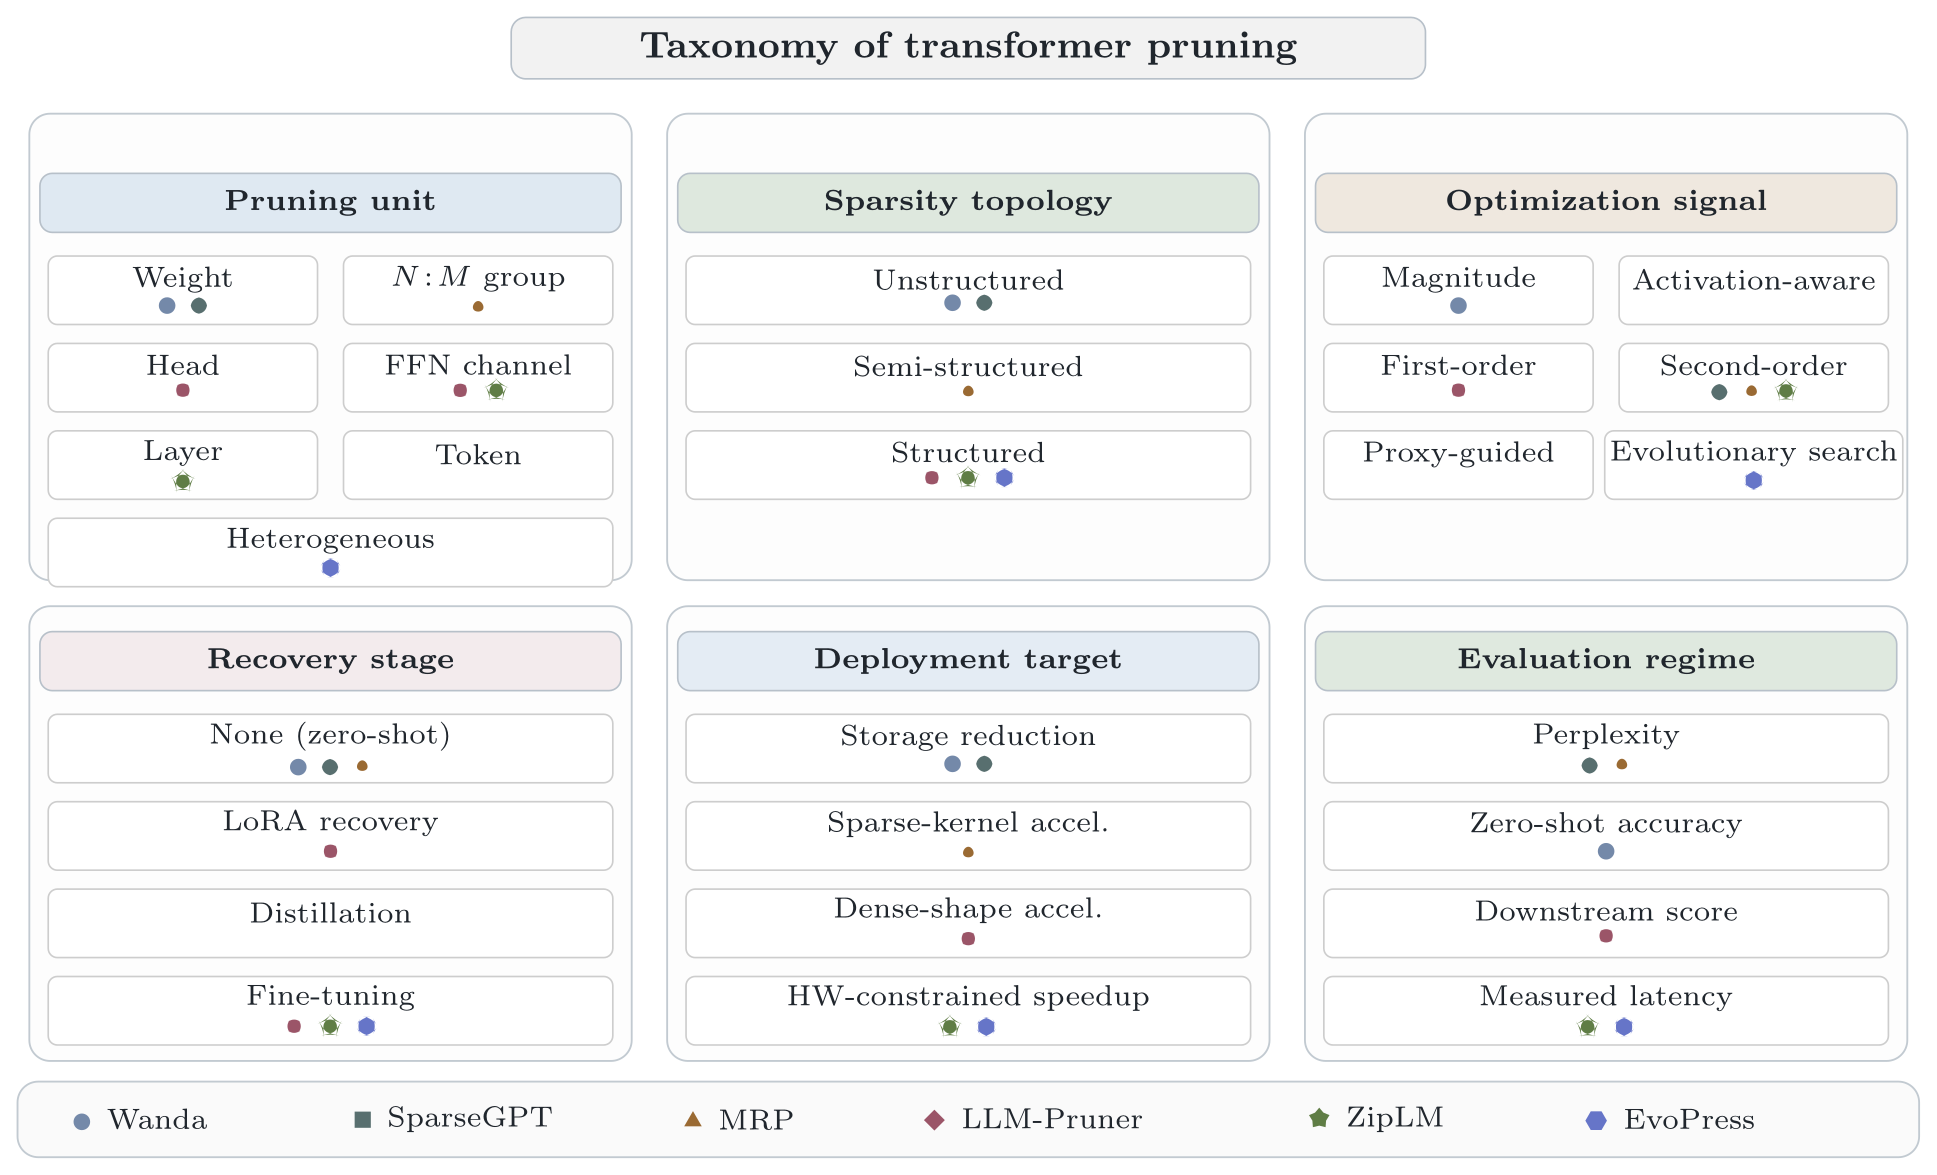
\includegraphics[width=\textwidth, height=0.88\textheight, keepaspectratio]{figures/compression/transformer_pruning_taxonomy.png}
	\caption{Classification of pruning methods by the unit of removal, sparsity topology, optimization signal, recovery stage, and primary deployment claim}
	\label{fig:pruning_taxonomy}
\end{figure}

\begin{table}[H]
	\centering
	\caption{Summary of pruning methods by unit, topology, signal, recovery, and deployment claim}
	\label{tab:pruning_taxonomy}
	\begin{tabularx}{\textwidth}{@{}l >{\raggedright\arraybackslash}X >{\raggedright\arraybackslash}X >{\raggedright\arraybackslash}X >{\raggedright\arraybackslash}X >{\raggedright\arraybackslash}X@{}}
		\toprule
		\textbf{Method} & \textbf{Unit} & \textbf{Topology} & \textbf{Signal} & \textbf{Recovery} & \textbf{Primary deployment claim} \\
		\midrule
		Wanda & Weight & Unstructured & Activation-aware saliency & None & Storage-oriented sparsity with strong zero-shot perplexity retention \\
		SparseGPT & Weight & Unstructured & Single-weight second-order compensation & None & High-sparsity pruning with local reconstruction \\
		CoFi & Layers / heads / FFN / hidden dimensions & Structured & Learned hard-concrete masks with $L_0$ control and distillation & Full task-specific pruning and fine-tuning & Dense-shape acceleration through jointly pruned Transformer structure \\
		LLM-Pruner & Heads / channels / blocks & Structured & First-order Taylor scoring with dependency groups & LoRA recovery & Structural compression with dense-shape execution \\
		Fast post-training pruning & Heads / FFN filters & Structured & Fisher-based constrained mask optimization & None beyond mask tuning & FLOPs- or latency-constrained structured pruning without retraining \\
		ZipLM & Heads / FFN dimensions & Structured & Second-order structured saliency with runtime-constrained search & Gradual fine-tuning and distillation & Measured speedup under device-specific constraints \\
		EvoPress / DarwinLM & Layer-wise compression levels & Heterogeneous structured & Proxy-guided or evolutionary search & Search-time evaluation or proxy training & Global configuration search under budget and hardware constraints \\
		\bottomrule
	\end{tabularx}
\end{table}

Figure~\ref{fig:pruning_taxonomy} separates the pruning literature by the unit being removed and by the metric used to decide removal. Table~\ref{tab:pruning_taxonomy} then makes this map concrete by assigning each reviewed method to a pruning unit, topology, scoring mechanism, recovery regime, and deployment claim.

Guided by this taxonomy, the remainder of this chapter reviews methods that prioritize maximum theoretical flexibility and search space exploration: Unstructured and Heterogeneous Search-based methods (Wanda, SparseGPT, EvoPress, and DarwinLM). Structured methods are reviewed in Chapter~\ref{chap:related_work_pruning_structured}.

\section{Saliency-Based Unstructured Methods}

Recall from Section~\ref{sec:pruning_criteria} that the Taylor expansion of the
loss change induced by pruning a weight $\theta_i$ produces a first-order term
proportional to the gradient and a second-order term capturing curvature
(Equation~\eqref{eq:taylor}). Saliency-based methods discard both terms and
instead use the weight magnitude or a proxy derived from activation statistics
as a surrogate for the true loss change. This zeroth-order approximation
requires no gradient computation and no calibration beyond a simple forward
pass, making these methods the cheapest option in the taxonomy.

\subsubsection{Magnitude and Activation-Aware Baselines}

\paragraph{Weight-Magnitude Pruning.}
Magnitude pruning uses absolute weight values as the saliency proxy:
\begin{equation}
	\mathcal{S}^{\mathrm{mag}}_{i,j} = |W_{i,j}|.
\end{equation}
Its core assumption is that small weights contribute less to the output and can be removed with limited degradation. The method requires no gradient-based recovery and remains the simplest baseline against which more sophisticated algorithms are evaluated.

\methodsep

\paragraph{Wanda (Weights $\times$ Activations).}
Wanda \cite{sun2023simple} refines this baseline by incorporating activation information from a small calibration set. The saliency score is
\begin{equation}
	\mathcal{S}^{\mathrm{wanda}}_{i,j} = |W_{i,j}| \cdot \|x_j\|_2,
\end{equation}
where $x_j$ is the $j$-th input activation channel and $\|x_j\|_2$ is its RMS norm estimated over $N$ calibration samples. The key insight is that importance is jointly encoded in weight magnitude and the energy of the coupled input channel.

\methoddetail{Algorithm Overview}
Both magnitude pruning and Wanda are one-shot post-training methods in the regime of Section~\ref{sec:post_training_pruning}: scores are computed once and no recovery training is applied afterward. Wanda processes each layer independently: it collects input activations on a small calibration set (typically 128 samples), computes per-weight saliency scores as the product of weight magnitude and activation norm, then prunes the lowest-scoring weights for each output neuron until the target sparsity $p$ is reached. No weight update or recovery step is applied. Magnitude pruning is a pure linear scan $O(|W|)$ with no calibration; Wanda adds only an activation-collection pass, keeping the overall cost near-linear.

These saliency methods are useful because they are cheap and easy to apply, but their decisions remain local. Once pruning moves from individual weights to heads, FFN channels, or layers, the method must account for structural dependencies between parameters. This motivates gradient-based structured pruning methods, where the score is computed over groups that can be removed consistently.

\methodsep

\section{Second-Order Unstructured Methods \& Semi-Structured Methods}
While magnitude and Wanda are purely zeroth-order, second-order methods such as SparseGPT \cite{frantar2023sparsegpt} and MRP \cite{kwon2022fast} attempt to capture curvature information to improve pruning decisions. SparseGPT estimates the Hessian of the loss with respect to weights using a block-wise approximation and applies a closed-form compensation to the remaining weights after pruning. MRP extends this idea to N:M sparsity patterns, where groups of weights are pruned together, and updates the compensation iteratively as more groups are removed. These methods are more expensive than local scoring but can achieve higher accuracy at high sparsity levels by accounting for the interactions between pruned and retained weights. However, they still operate at the weight level and do not consider the structural dependencies that arise when pruning entire heads, channels, or layers. This motivates the next family of methods that optimize for structured pruning with gradient-based criteria and recovery.

\subsection{Optimal Brain Compression Formulation}

For a layer with weight matrix $\mathbf{W} \in \mathbb{R}^{d_{\text{out}} \times d_{\text{in}}}$ and calibration activations $\mathbf{X} \in \mathbb{R}^{d_{\text{in}} \times n}$, the layer-wise sparse reconstruction problem is
\begin{equation}
	\min_{\mathbf{W}^{\text{sparse}}}
	\|\mathbf{W}\mathbf{X} - \mathbf{W}^{\text{sparse}}\mathbf{X}\|_F^2
	\quad \text{s.t.} \quad
	\|\mathbf{W}^{\text{sparse}}\|_0 \leq (1-p)\, d_{\text{out}} d_{\text{in}},
\end{equation}
where $\|\cdot\|_F$ is the Frobenius norm, $\|\cdot\|_0$ counts the number of nonzero entries, and $p \in (0,1)$ is the target sparsity ratio. Using the empirical Hessian proxy $\mathbf{H} = \mathbf{X}\mathbf{X}^T / n$, this becomes a curvature-aware reconstruction problem whose solution depends on $\mathbf{H}^{-1}$ to redistribute pruning error across remaining weights. The methods that follow differ in how they instantiate this objective: SparseGPT removes one scalar weight at a time, MRP removes an entire N:M group jointly, Fisher-based pruning applies curvature scoring to structured masks, and ZipLM extends the same principle to executable Transformer structures under runtime constraints.

\subsection{Single-Weight Iterative Removal (SparseGPT)}

SparseGPT \cite{frantar2023sparsegpt} greedily prunes one weight at a time while applying compensation updates to remaining weights in the current block. This can be read as a blockwise version of the OBS correction introduced in Section~\ref{subsec:obd_obs} and formalised for large linear layers in Section~\ref{subsec:second_order_criteria}. Its local objective at iteration $t$ is
\begin{equation}\label{eq:srp}
	\min_{\delta w} \frac{1}{2}\delta w^T H \delta w
	\quad\text{s.t.}\quad
	(w+\delta w)\cdot e_t = 0,
\end{equation}
where $e_t$ is the one-hot selector for the pruned weight.

\methoddetail{Algorithm Overview}
SparseGPT is a post-training one-shot method in the regime of Section~\ref{sec:post_training_pruning}: pruning and compensation are applied in a single forward pass over the layers without any subsequent gradient-based recovery. It processes the weight matrix in column blocks of size $B$. For each block, it first constructs the regularized inverse Hessian $(XX^T + \lambda I)^{-1}$. Within each block, it iteratively identifies the weight with minimum local second-order loss, sets it to zero, then updates the remaining weights in that block using the corresponding column of $\mathbf{H}^{-1}$. After processing a block, lazy batch updates are applied to adjacent blocks. The method scales as $O(d_{\text{in}}^2 d_{\text{out}} + d_{\text{in}}^3/B)$ per layer, with a calibration budget of approximately 128 samples.

It is more instructive to understand SparseGPT as a weight-level, Hessian-compensated method for pruning: each decision to prune weights is made locally, and weights are updated to make the layer output's deviation as minimal as possible \cite{frantar2023sparsegpt}. It is through this same lens that SparseGPT's modification for semi-structured N:M sparsity can be understood, where the compensation method is kept and mask selection is constrained to local groups. If the block size is set to $B_s = M$, and from each group of $M$ weights the $N$ weights with the smallest OBS reconstruction score are selected for removal, the compensation becomes more localized to a block instead of applying it for the whole layer. Within that block, however, weights are still selected and compensated one at a time, so the compensation at each step does not account for the interactions among the other weights being simultaneously removed from the same group, which is the gap MRP directly addresses.

\methodsep

\subsection{Joint Optimization for Multi-Weight Removal (MRP)}

The MRP framework \cite{zhao2024pruning} generalizes second-order pruning to N:M groups. For a vectorized weight block $w$ and binary pruning mask $M$, where $M_i=1$ indicates that weight $i$ is pruned, the objective minimizes the second-order loss increase for the full group:
\begin{equation}\label{eq:ptp}
	\min_{\delta w} \frac{1}{2}\delta w^T H \delta w + g^T \delta w
	\quad\text{s.t.}\quad
	(w+\delta w)\odot M = 0,
\end{equation}
where $g$ is the gradient of the loss with respect to $w$, and $\odot$ denotes elementwise multiplication. Solving the group jointly yields a compensation update for the retained weights:
\begin{equation}
	\delta w^\star = -H_{\bar{M}\bar{M}}^{-1}(g_{\bar{M}} + H_{\bar{M}M}w_M),
\end{equation}
where $M$ denotes pruned indices, $\bar{M}$ retained indices, and $w_M$ the weight values at the pruned coordinates. This expression makes the role of the block Hessian explicit: in N:M pruning, the removed weights are not independent decisions, so compensation must be computed for the group.

\methoddetail{Algorithm Overview}
MRP is a post-training one-shot method in the regime of Section~\ref{sec:post_training_pruning}: no gradient updates or recovery training are applied after pruning. It operates layer by layer. For each layer, the block Hessian is estimated from calibration activations. The weight tensor is partitioned into non-overlapping groups of $M$ consecutive weights. For each group, the joint second-order problem is solved: the mask selecting the $M-N$ weights with the highest reconstruction cost is identified, and the compensation update $\delta w^\star$ is applied to the retained $N$ weights before the next group is processed. Because the group is treated as a group, the method correctly accounts for interactions among simultaneously pruned coordinates within the block.

Figure~\ref{fig:hessian_compensation} illustrates this difference. SparseGPT compensates after removing one scalar weight, whereas MRP compensates after removing a constrained local group. The figure is therefore used to distinguish scalar second-order correction from group-level second-order correction.

\begin{figure}[H]
\centering
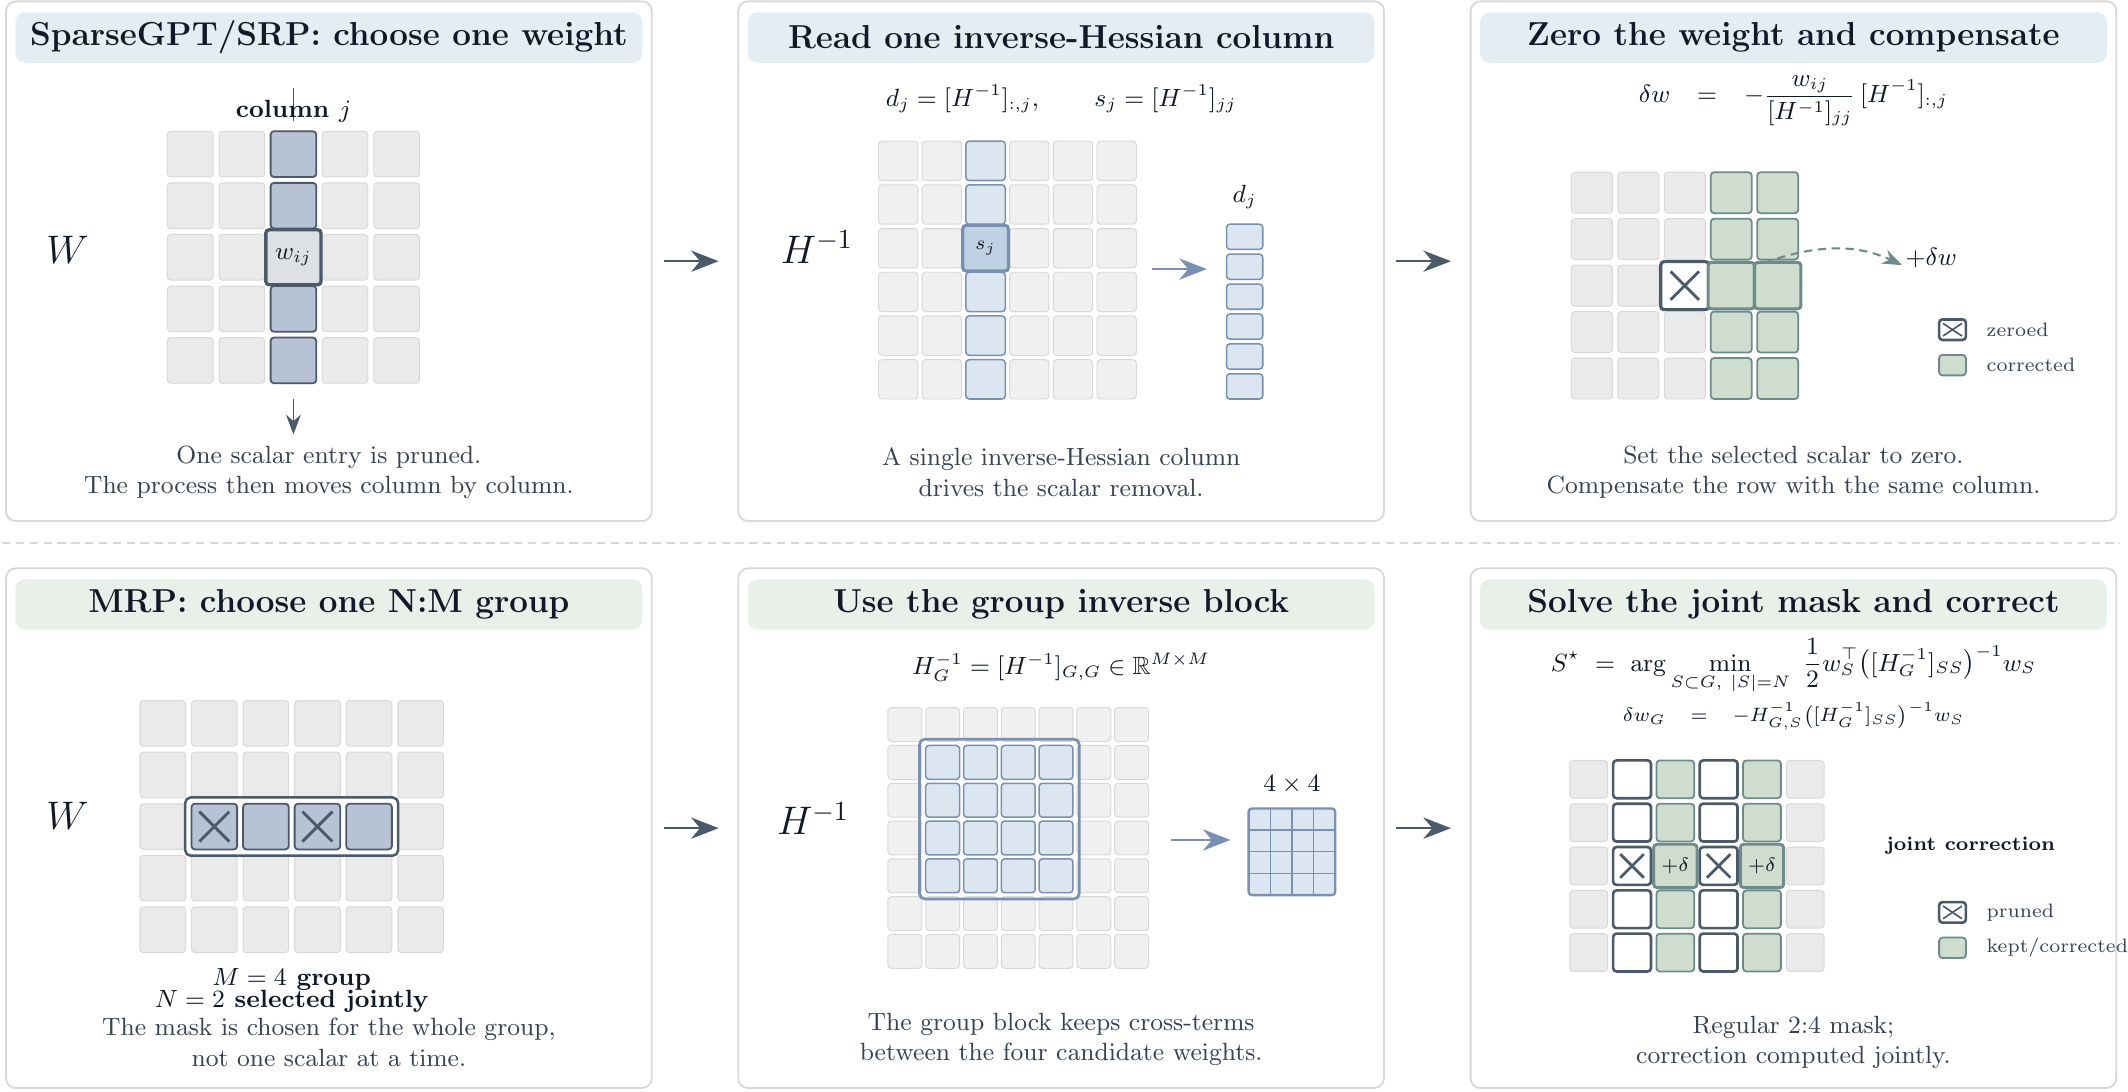
\includegraphics[width=0.8\linewidth]{figures/compression/sparsegpt_mrp_compensation.png}
\caption[Second-order compensation strategies for unstructured and semi-structured pruning.]{Second-order compensation strategies for unstructured and semi-structured pruning.}
\label{fig:hessian_compensation}
\end{figure}

\methodsep
\section{Search-Based Heterogeneous Methods}

Search-based methods operate over complete sparsity configurations instead of the aforementioned application of a single closed-form ranking rule to individual units. This is especially relevant when the quality of a pruning decision depends on how several removals interact across layers. Search-based methods are more expensive than local scoring, but they can explore a much larger space of configurations and find better-performing candidates at high compression levels. The two representative methods reviewed here are EvoPress, which performs an evolutionary search over discrete layer-wise compression profiles, and DarwinLM, which extends this search to structured pruning with training-aware selection.
\paragraph{EvoPress.}
EvoPress \cite{evopress2024} searches over discrete layer-wise compression profiles instead of assigning a single saliency score per layer. A candidate is a configuration $\mathbf{C} = \{c_1,\dots,c_L\}$ where $c_\ell \in \mathcal{S}_\ell$ is the compression level for layer $\ell$. Budget is preserved by level-switch mutation: one layer becomes more compressed only if another becomes less compressed, keeping the global average sparsity $S_{\text{glob}}$ fixed. Mutations are deliberately local, with most offspring differing from the parent by only one or two switches.

Selection proceeds in multiple rounds with increasing token budgets and decreasing survivor counts:
\begin{equation}
	\mathcal{P}^{(r+1)} =
	\operatorname{Top}_{n_{r+1}}
	\left(
	\left\{
	\mathcal{F}_{T_r}(C) \mid C \in \mathcal{P}^{(r)}
	\right\}
	\right),
	\qquad
	T_1<T_2<\cdots,\;
	n_1>n_2>\cdots,
\end{equation}
where the fitness signal is KL divergence to the reference model. This progressive evaluation scheme is what makes EvoPress practically efficient: early rounds use few tokens to discard poor candidates quickly, reserving the full calibration budget for finalists. The method converges in approximately 5--6 GPU hours for a standard Llama-2-7B sparsity search.

Figure~\ref{fig:evolutionary_pruning_flow} summarizes this search loop. The important point is that the algorithm evaluates complete compression profiles, selects promising candidates with increasing evaluation budgets, and mutates the retained profile while preserving the global compression constraint.

\begin{figure}[H]
\centering
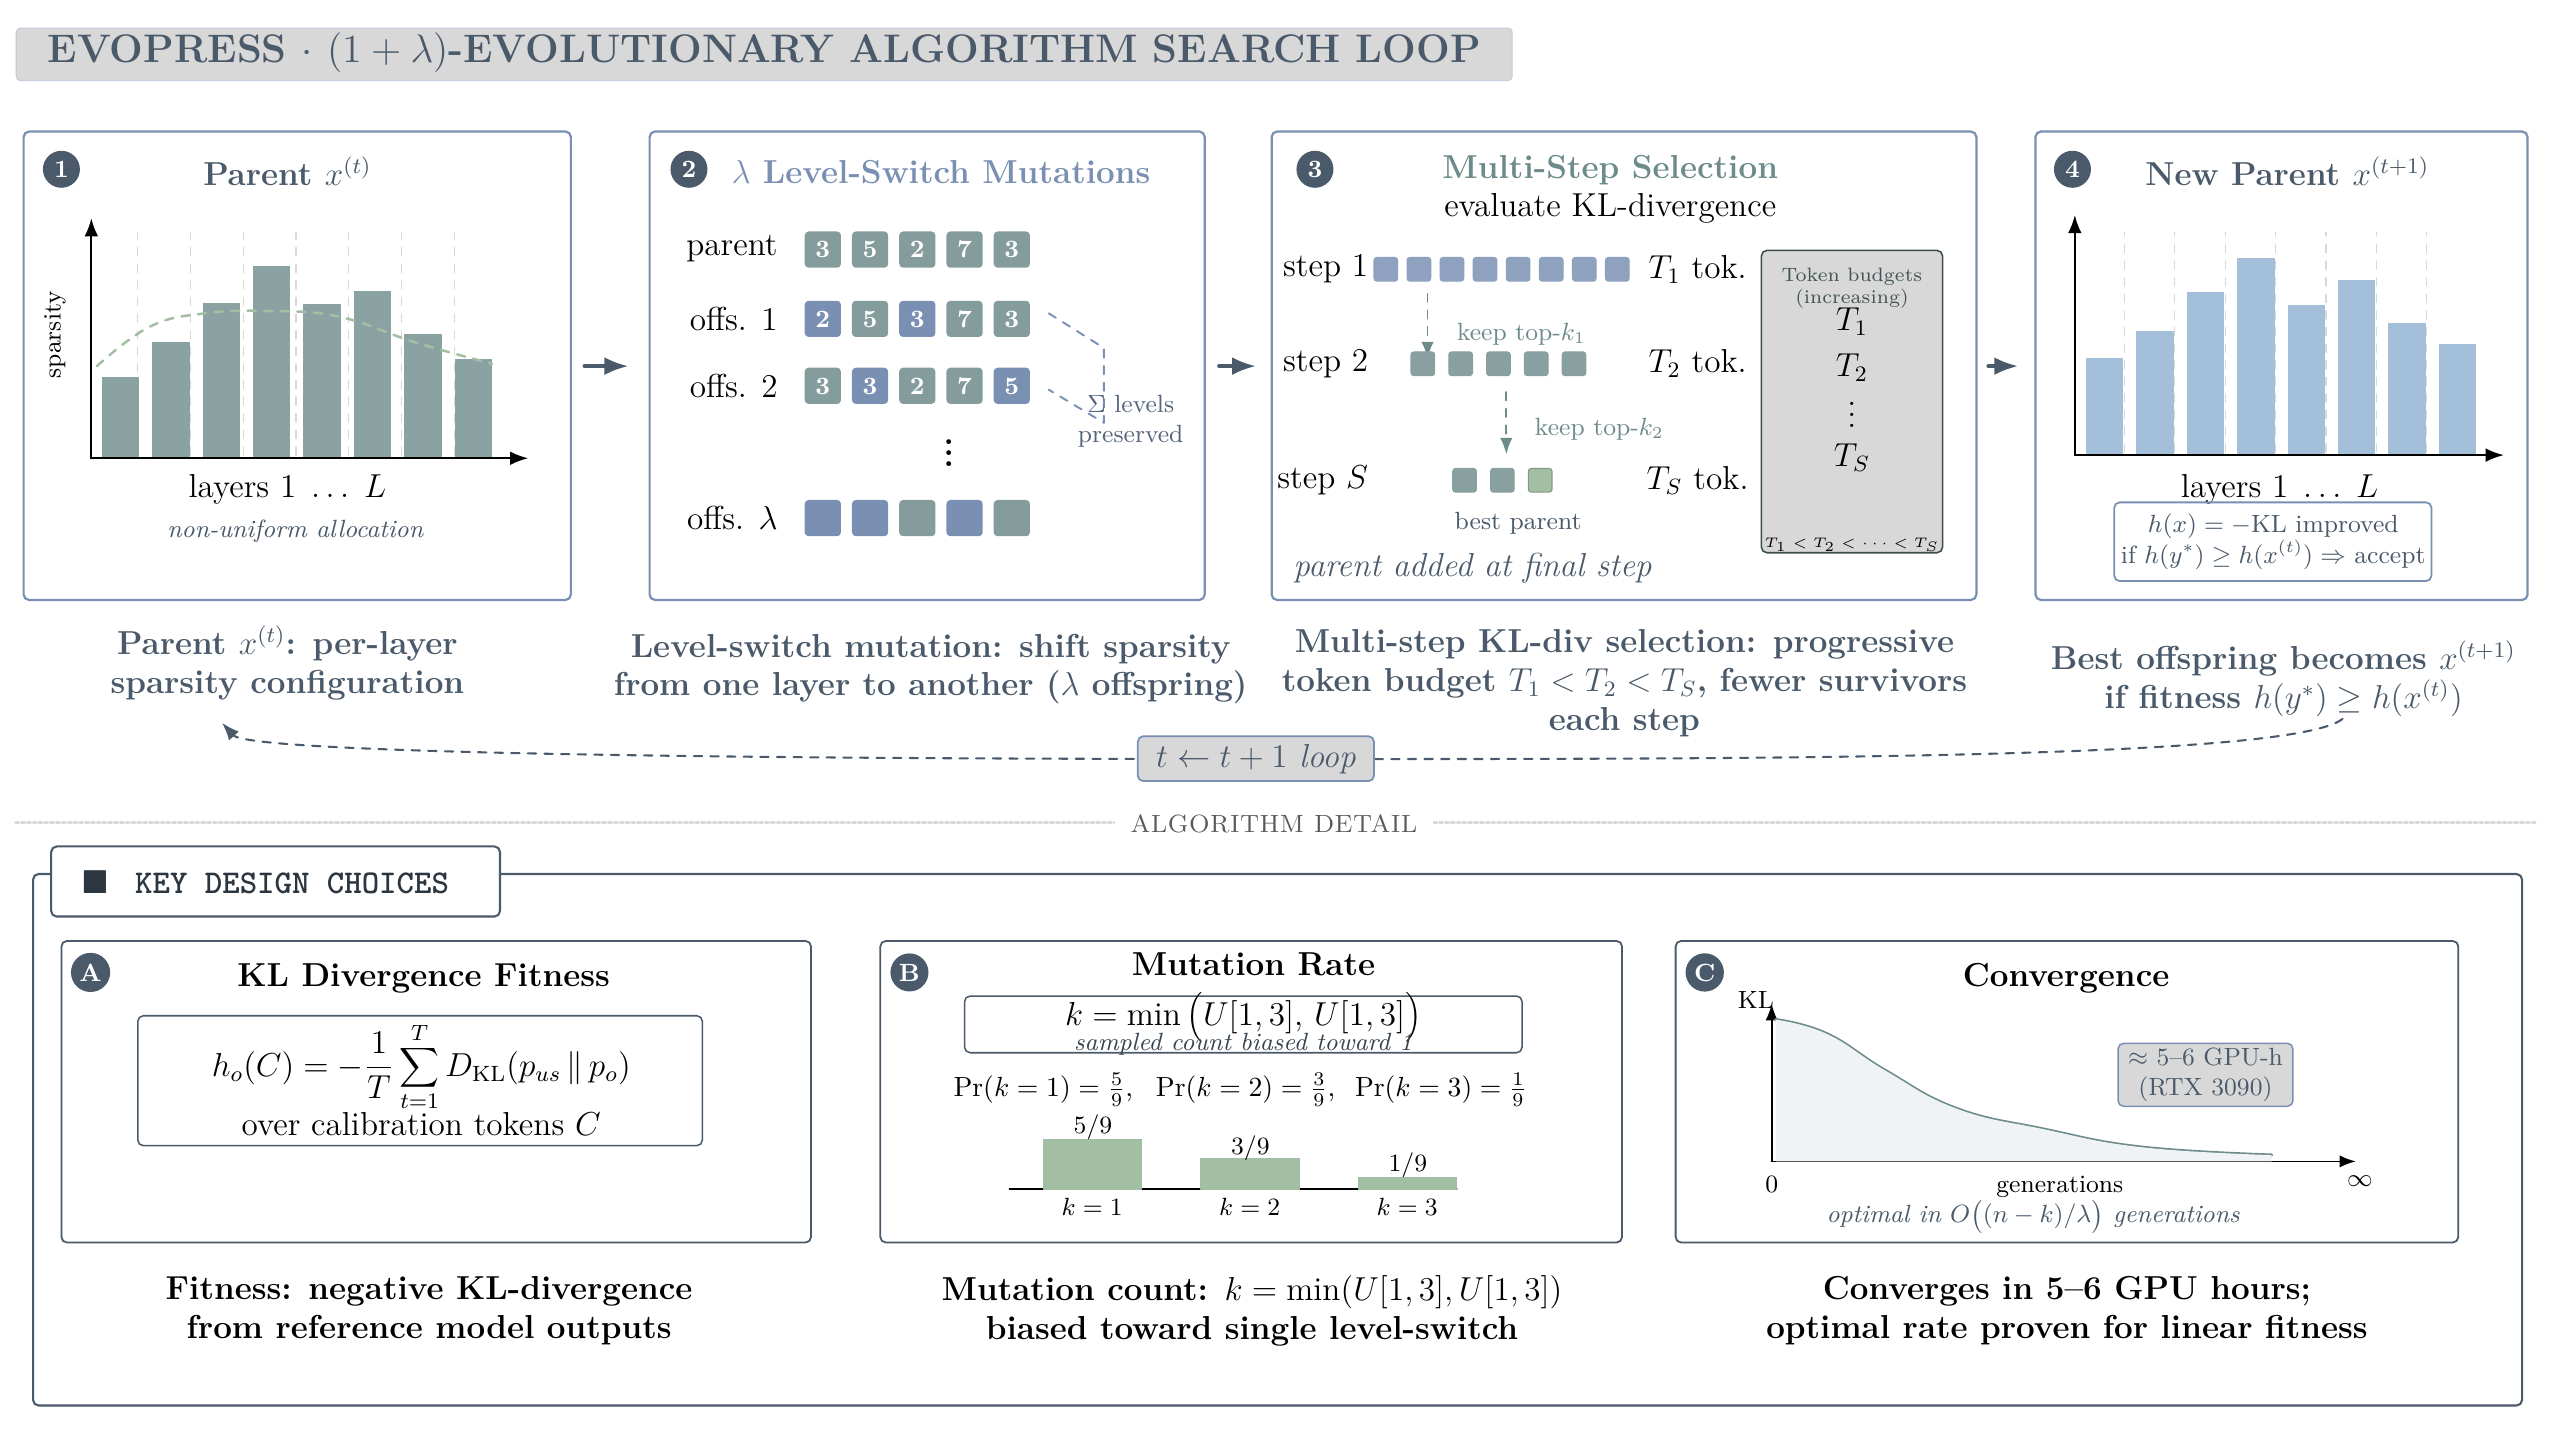
\includegraphics[width=0.94\linewidth,height=0.50\textheight,keepaspectratio]{figures/compression/evopress_search_loop.png}
\caption[EvoPress $(1+\lambda)$ evolutionary search loop for dynamic LLM compression \citep{evopress2024}.]{EvoPress $(1+\lambda)$ evolutionary search loop for dynamic LLM compression \citep{evopress2024}. The method applies budget-preserving level-switch mutation and progressively evaluates candidates with larger calibration budgets.}
\label{fig:evolutionary_pruning_flow}
\end{figure}
\FloatBarrier

\methodsep

\paragraph{DarwinLM.}
DarwinLM \cite{darwinlm2025} extends evolutionary search to \emph{structured} pruning by unifying OBS-style second-order pruning with a training-aware offspring selection strategy. It differs from EvoPress on three axes: structured granularity (heads and FFN channels), front-loaded Hessian computation stored in a sparsity-level database (SLD), and fitness measured after a short lightweight finetune.

\methoddetail{Sparsity Level Database}
For each module, DarwinLM solves the structured OBS problem at $N_l$ equally-spaced sparsity levels and stores the pruned-and-compensated weights. The optimal structured mask and compensation are:
\begin{align}
	M^* &= \arg\min_{M}\sum_{i=1}^{d_{\mathrm{row}}}
		\mathbf{W}_{i,M}\bigl(\hat{H}^{-1}_{MM}\bigr)^{-1}\mathbf{W}_{i,M}^\top, \\
	\delta^* &= -\mathbf{W}_{:,M}\bigl(\hat{H}^{-1}_{MM}\bigr)^{-1}\hat{H}^{-1}_{M,:},
\end{align}
where $d_{\mathrm{row}}$ is the output dimension of the module weight matrix, $M$ indexes the pruned columns, and $\hat{H}$ is the empirical Hessian computed from calibration activations. During search, candidate models are assembled by looking up stored entries, avoiding any Hessian recomputation.

\methoddetail{Training-Aware Selection}
Each candidate receives a short lightweight finetune before evaluation:
\begin{equation}
	\mathcal{F}(C_k) = D_{\mathrm{KL}}\!\bigl(\hat{M}\,\|\,\operatorname{finetune}(C_k,\, T_f)\bigr),
\end{equation}
where $\hat{M}$ is the output distribution of the dense reference model and $T_f$ is the fine-tuning token budget. Selection uses three progressive rounds ($T_f \in \{10\text{K}, 50\text{K}, 200\text{K}\}$ tokens) with decreasing survivor counts. The SLD must be computed once per model and sparsity range, making the upfront cost proportional to $L \cdot N_l$ structured OBS operations. DarwinLM compresses Llama-2-7B to 2.7B parameters with higher downstream accuracy than ShearedLlama using $5\times$ fewer post-training tokens (10B vs.\ 50B).

\methoddetail{Algorithm Overview}
DarwinLM sits between a post-training and an iterative regime: the SLD is built offline without end-to-end training, but each search candidate receives a lightweight fine-tune before fitness evaluation. In the offline phase, the SLD is built: for each module and each of $N_l$ sparsity levels, the structured OBS problem is solved and the pruned-and-compensated weights are stored, so that any candidate configuration can be assembled by table lookup. In the search phase, candidate models are stitched together by selecting one SLD entry per module, then evaluated through that lightweight finetune. Mutation follows the same budget-preserving logic as EvoPress, swapping one module's sparsity level up only if another's is swapped down. Selection proceeds over three rounds with token budgets of 10K, 50K, and 200K and shrinking survivor counts, so weaker candidates are eliminated cheaply before the full evaluation budget is spent. The upfront SLD cost is proportional to $L \cdot N_l$ structured OBS operations and is paid once per model.

Figure~\ref{fig:darwinlm_pruning_flow} shows the corresponding DarwinLM workflow. Compared with EvoPress, the key visual distinction is the front-loaded sparsity-level database: candidate models are assembled from stored structured-pruning choices, then filtered through training-aware selection.

\begin{figure}[H]
\centering
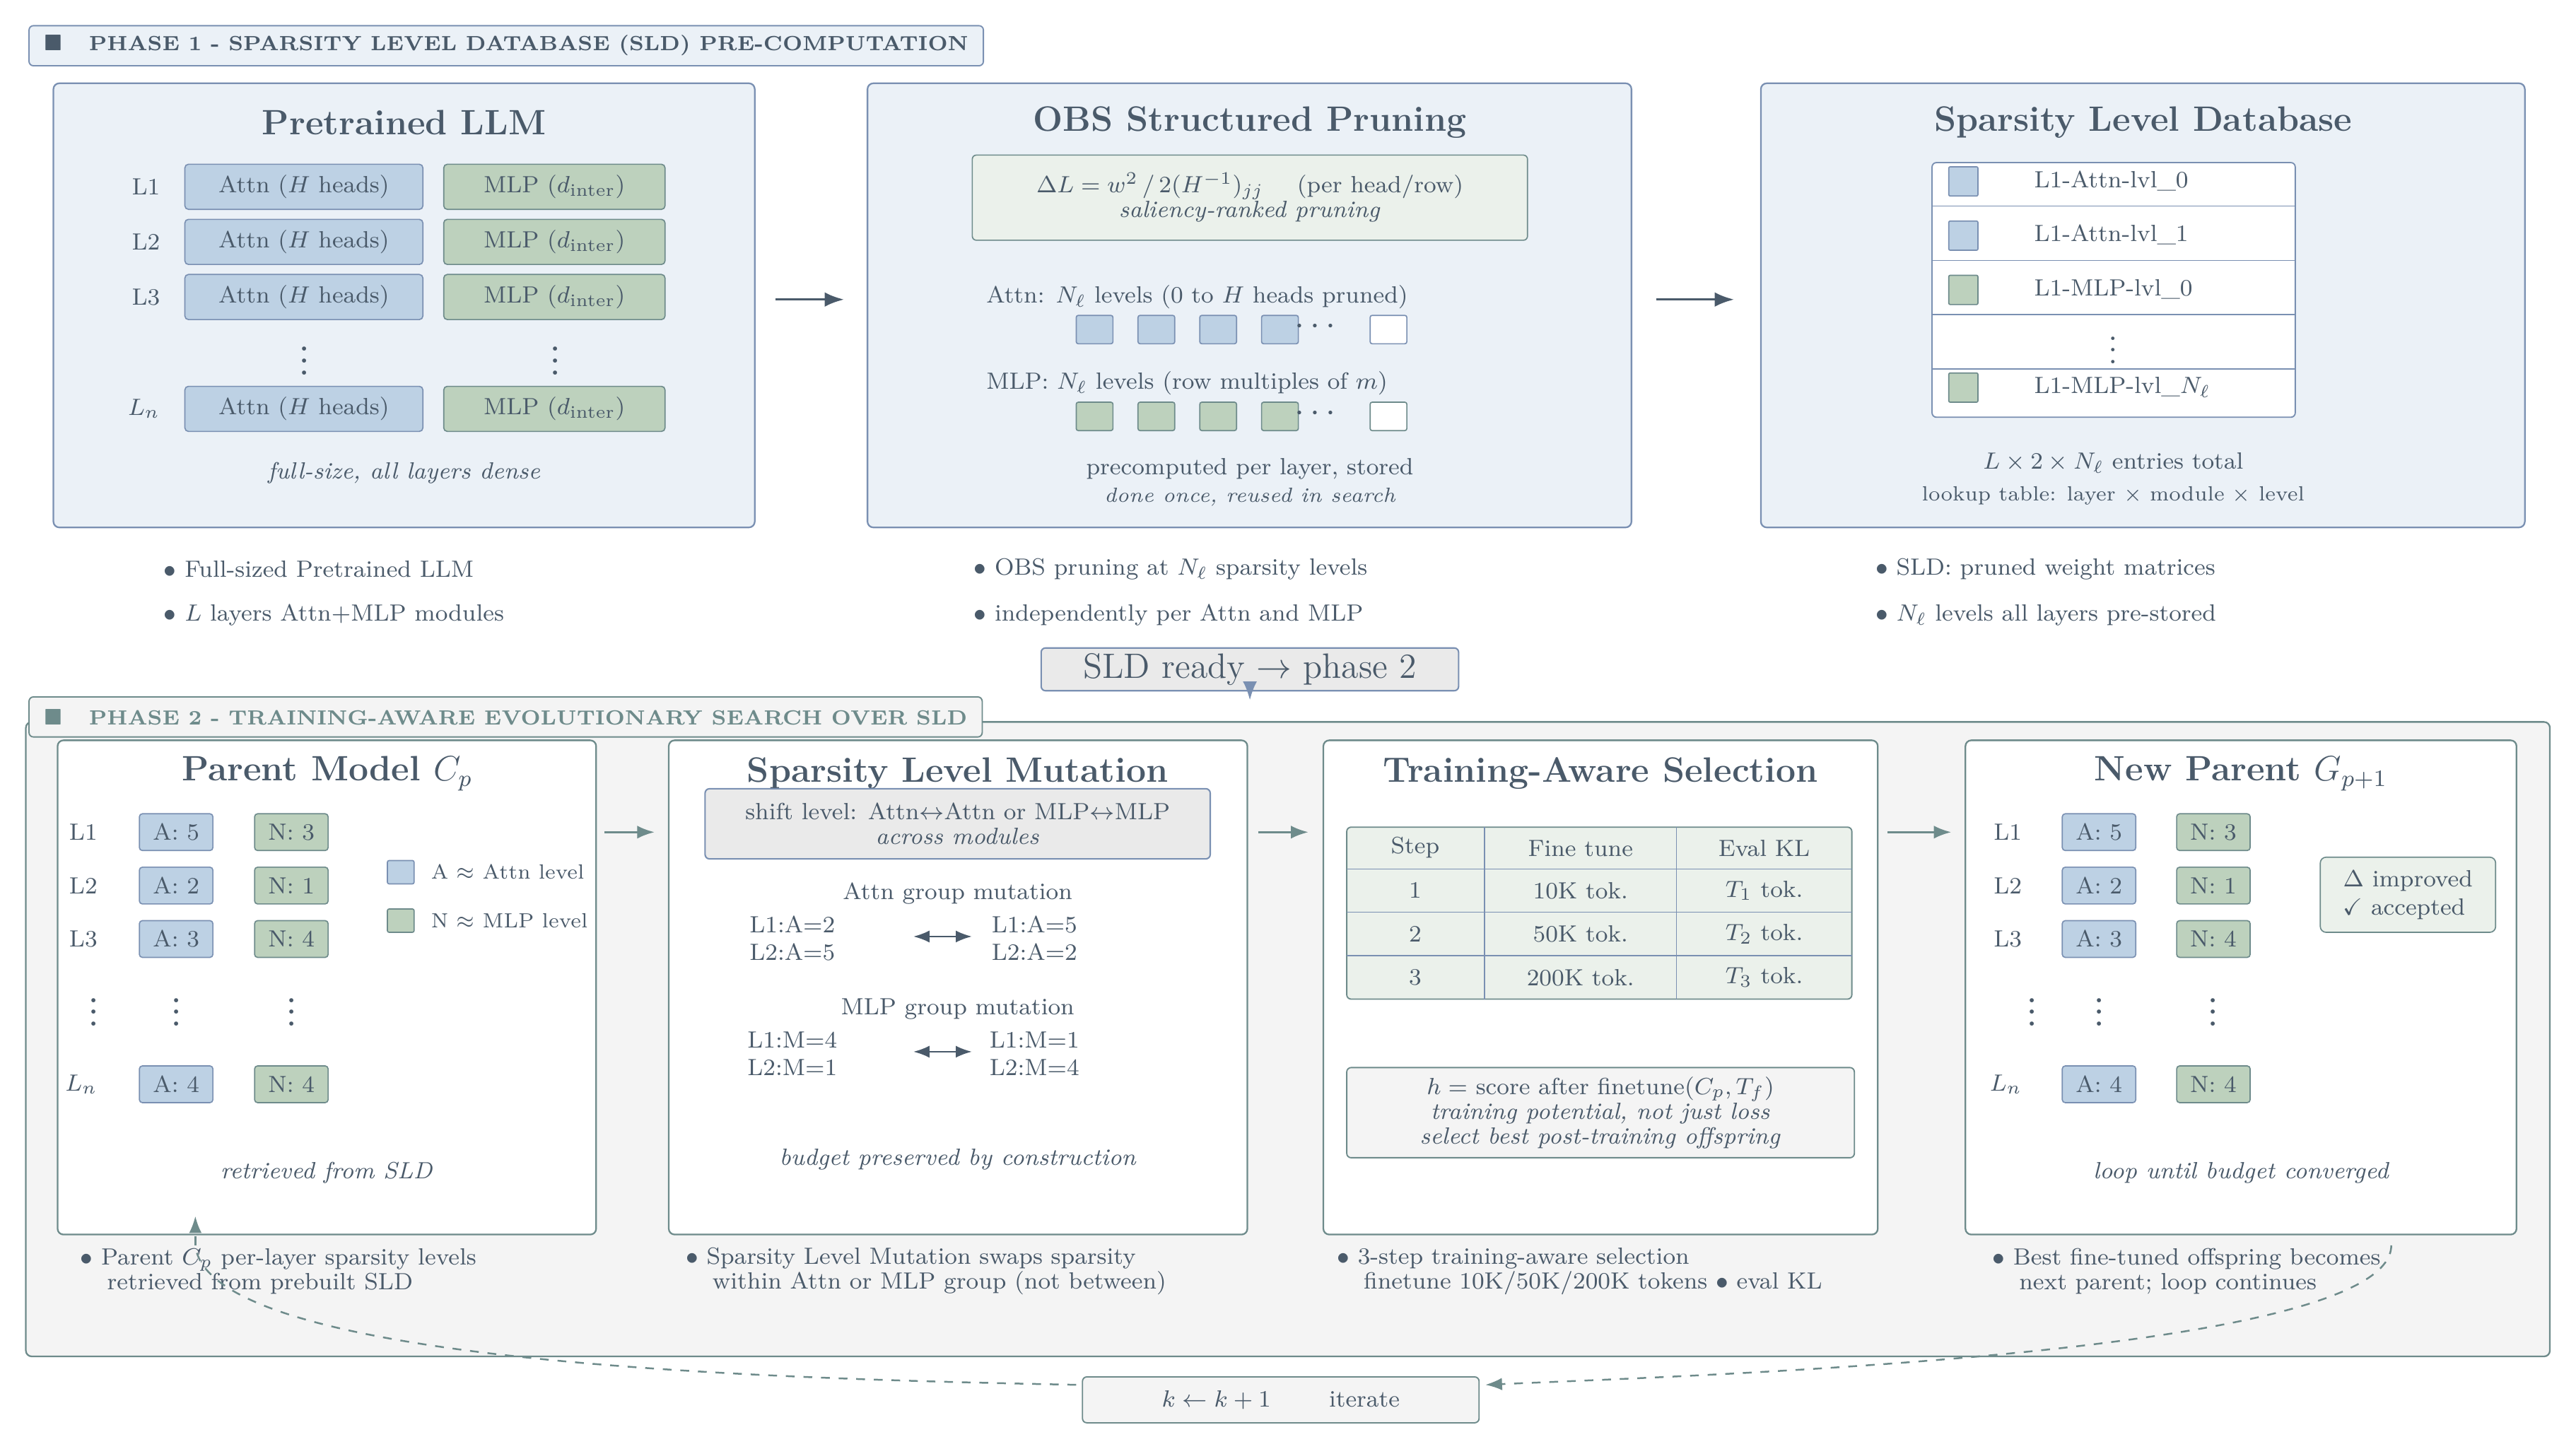
\includegraphics[width=0.94\linewidth,height=0.50\textheight,keepaspectratio]{figures/compression/darwinlm_search_loop.png}
\caption[DarwinLM search loop \citep{darwinlm2025}.]{DarwinLM search loop \citep{darwinlm2025}. The method first builds a sparsity-level database with OBS-style structured pruning, then performs training-aware evolutionary selection over stitched candidate models.}
\label{fig:darwinlm_pruning_flow}
\end{figure}

\FloatBarrier

Table~\ref{tab:preparation_cost_profile} compares the practical preparation cost of the reviewed families. This table is included separately from the empirical results because a method can report strong accuracy while still requiring a substantially different calibration, recovery, benchmarking, or search budget.

\begin{table}[H]
	\centering
	\caption[Preparation cost and evaluation requirements of representative pruning methods.]{Preparation cost and evaluation requirements of representative pruning methods. The table separates low-cost post-training scoring, training-dependent structured pruning, curvature-based reconstruction, and population-based search.}
	\label{tab:preparation_cost_profile}
	\begin{tabularx}{\textwidth}{@{}>{\raggedright\arraybackslash}p{2.6cm}LL@{}}
		\toprule
		\textbf{Method} & \textbf{Dominant preprocessing cost} & \textbf{Additional requirement} \\ \midrule
		Magnitude & Linear scan $O(|W|)$ & None \\
		Wanda & Activation collection and linear scoring & Small calibration set ($\approx$128 samples) \\
		CoFi & Multi-epoch joint mask and weight optimization & Task-specific teacher; $\approx$33 h for MNLI \\
		LLM-Pruner & Forward/backward scoring over dependency groups & LoRA recovery ($\approx$2.5 h on RTX 4090) \\
		SparseGPT & Block-wise Hessian estimation and reconstruction & Calibration Hessian \\
		MRP & Group-wise mask search and compensation & Block curvature updates for N:M groups \\
		Fast PTPF & Diagonal or block Fisher estimation with mask tuning & Calibration set; optional latency lookup table \\
		ZipLM & Layer-wise Hessian updates and runtime-table search & Calibration set plus hardware benchmarking pass \\
		EvoPress / DarwinLM & Population search over compression profiles & 1--6 GPU-hours; SLD pre-computation for DarwinLM \\ \bottomrule
	\end{tabularx}
\end{table}



\section{Conclusion}
We have reviewd in the chapter the pruning methods that prioritize theoretical flexibility and search space exploration, formally known as Unstructured and Heterogeneous Search-based methods. Unstructured methods such as Wanda and SparseGPT primarily optimize weight-level saliency, while search-based methods such as EvoPress and DarwinLM treat pruning as configuration optimization under explicit budget or hardware constraints. Those methods are especially relevant for high-sparsity regimes, where the quality of pruning decisions depends on how several removals interact across layers. Search-based methods are more expensive than local scoring, but they can explore a much larger space of configurations and find better-performing candidates at high compression levels. The next chapter will review structured methods that optimize for dense-shape acceleration through joint pruning of executable structures such as attention heads, FFN channels, and layers.
	\providecommand{\methoddetail}[1]{}
\providecommand{\methodsep}{}
\chapter{Related work on pruning: Structured Methods}
\label{chap:related_work_pruning_structured}


\section{Introduction}
While Chapter \ref{chap:related_work_pruning_unstructured} explored methods that remove individual weights or apply heterogeneous sparsity profiles, those approaches often rely on specialized sparse-execution hardware to achieve real-world latency reductions. This chapter shifts focus to the other side of our taxonomy: Structured Pruning.

Instead of scattering zeros throughout a weight matrix, structured pruning removes entire executable units such as attention heads, feed-forward channels, or complete Transformer layers. By excising these structural blocks, the resulting compressed model remains a standard, albeit smaller, dense neural network. This allows it to be accelerated on any standard hardware using highly optimized dense matrix multiplications, achieving immediate out-of-the-box speedups.

However, removing entire structural units is highly destructive to the model's forward pass, making the criteria for removal significantly more complex than unstructured weight magnitude. Based on the taxonomy established previously, this chapter reviews four prominent structured pruning methodologies: LLM-Pruner, CoFi, Fast Post-Training Pruning (Fast PTPF), and ZipLM. These methods represent the state-of-the-art in overcoming the destructive nature of structured removals, utilizing dependency graphs, learnable masks, and second-order optimization.

\section{Gradient-Based Methods}

The first order term of the Taylor expansion (Equation~\eqref{eq:taylor}) retains a value that is a product of the gradient and the weight value. The criterion thus becomes sensitive to the direction of loss change as well as the weight magnitude. The methods in this section utilize precisely this first order signal, however instead of single values it utilizes grouped structure, for example heads, channels and blocks.

Structured pruning replaces individual-weight saliency with group-level importance, because the natural units in a Transformer, namely attention heads, FFN channels, and entire layers, are coupled through residual pathways and shared projection matrices. Removing one head, for example, requires deleting consistent slices from $W_Q$, $W_K$, $W_V$, and $W_O$ together; removing an FFN channel removes coordinated rows and columns from the two projection matrices. Any pruning criterion applied at this level must therefore identify groups that can be removed as a unit without breaking the forward pass \cite{michel2022not,kurtic2022optimal}.

\paragraph{LLM-Pruner.}
LLM-Pruner \cite{ma2023llmpruner} addresses the dependency problem explicitly by constructing a graph over the neurons of the network. For neurons $N_i$ and $N_j$ with input set $\mathrm{In}(N)$ and output set $\mathrm{Out}(N)$, the graph encodes two rules:
\begin{align}
	N_j \in \mathrm{Out}(N_i) \wedge \deg^{-}(N_j)=1 &\implies N_j \text{ depends on } N_i, \label{eq:dep1}\\
	N_i \in \mathrm{In}(N_j) \wedge \deg^{+}(N_i)=1 &\implies N_i \text{ depends on } N_j. \label{eq:dep2}
\end{align}
Here $\deg^{-}(N_j)$ is the in-degree of $N_j$ (number of neurons feeding into it) and $\deg^{+}(N_i)$ is the out-degree of $N_i$. The transitive closure of these rules groups all coupled parameters into a single dependency group $\mathcal{G} = \{W_i\}_{i=1}^M$, which is the minimal unit that can be consistently removed.

Once groups are defined, each is scored using a first-order Taylor approximation of the loss increase over a small calibration set $\mathcal{D}$. The importance of a structure tensor $W_i$ is estimated as
\begin{equation}
	I_{W_i}
	\approx
	\left|
	\frac{\partial \mathcal{L}^{\top}(\mathcal{D})}{\partial W_i}W_i
	-\frac{1}{2}W_i^{\top}HW_i
	\right|,
	\label{eq:taylor-vector}
\end{equation}
where $H$ is the local Hessian. The first-order gradient is retained alongside the Hessian term because the calibration set is only a proxy for the pretraining distribution; discarding it would introduce bias. An element-wise variant replaces $H$ with a Fisher-diagonal approximation. Individual tensor scores within a group are aggregated by sum, product, max, or last-only operators, and groups with the lowest aggregate score are removed first.

LLM-Pruner sits between a post-training and a recovery regime: scoring is post-training and requires no gradient propagation through the full model, but the pruned network is then passed through a LoRA recovery stage in line with the iterative recovery approach of Section~\ref{subsec:iterative_pruning}. LoRA adapters \cite{hu2021lora} are inserted into all linear modules and fine-tuned for two epochs over roughly 50K samples. The low-rank factors are then merged back into the weight matrices, leaving no adapter overhead at inference time. The full scoring stage requires only 10 short calibration sequences, making the preprocessing cost modest relative to the recovery phase.

\methodsep

\paragraph{CoFi.}
CoFi \cite{xia2022structured} is the main structured-pruning example of the learnable-mask criteria introduced in Section~\ref{subsec:learnable_adaptive_criteria}. It places binary masks on attention blocks, heads, FFN blocks, intermediate channels, and the shared hidden dimension, then optimises these masks jointly with the task loss:
\begin{align}
	\mathrm{MHA}(X) &= z_{\mathrm{MHA}} \sum_{i=1}^{N_h} z_{\mathrm{head}}^{(i)} \,\mathrm{Att}\!\left(W_Q^{(i)},W_K^{(i)},W_V^{(i)},W_O^{(i)},X\right), \\
	\mathrm{FFN}(X) &= z_{\mathrm{FFN}}\, \mathrm{gelu}(XW_U)\,\mathrm{diag}(z_{\mathrm{int}})\,W_D,
\end{align}
where $N_h$ is the number of attention heads, $W_Q^{(i)}, W_K^{(i)}, W_V^{(i)}, W_O^{(i)}$ are the query, key, value, and output projection matrices of head $i$, and $W_U$, $W_D$ are the up- and down-projection matrices of the FFN. Each mask variable $z$ is relaxed to a continuous value during training using the hard-concrete distribution for $L_0$ regularisation, which allows gradients to flow through the mask. The training objective combines task loss with a distillation term and a Lagrangian sparsity constraint:
\begin{equation}
	\mathcal{L}_{\mathrm{prune}}
	=
	\mathcal{L}_{\mathrm{task}}
	+
	\mathcal{L}_{\mathrm{distil}}
	+
	\lambda_1(\hat s - s_0)
	+
	\lambda_2(\hat s - s_0)^2,
\end{equation}
where $s_0$ is the sparsity target and $\hat{s}$ is the expected sparsity under the current mask distribution. Because the masks at different granularities interact, CoFi can discover structured subnetworks that a simple per-group ranking would miss.

\methoddetail{Algorithm Overview}
CoFi is a training-time iterative method in the sense of Section~\ref{subsec:iterative_pruning} where mask decisions and weight updates are interleaved throughout training. A warm-up phase first stabilizes the model weights before mask learning begins, with the sparsity constraint applied softly. The main phase then jointly optimises masks and weights under the Lagrangian objective, progressively tightening the sparsity target toward $s_0$ over training. Once the target is reached, each continuous mask variable is thresholded against zero to produce a binary decision, and a final fine-tuning pass is run on the surviving subnetwork. Because masks at all granularities are trained simultaneously.

Gradient-based structured pruning improves the consistency of the removed units, but the score still depends on a local approximation of how removal affects the loss. When pruning becomes more aggressive, interactions among remaining and removed weights become more important. This leads to second-order methods, which use curvature information or local reconstruction objectives to compensate for the error introduced by pruning.



\section{Second-Order Structured Methods}

The second-order term of the Taylor expansion (Equation~\eqref{eq:taylor}) captures the curvature of the loss around the current weights. Retaining this term allows the
pruning criterion to account for how much a removal actually shifts the loss given the local geometry of the loss landscape. As discussed in Section~\ref{subsec:second_order_criteria}, this leads to the OBS framework, where the optimal weight correction after a removal is derived from the inverse Hessian. The methods in this section apply that same principle the scale of modern LLMs, recovering tractability by restricting the Hessian computation to individual layers or column blocks.

\subsection{Optimal Brain Compression Formulation}

For a layer with weight matrix $\mathbf{W} \in \mathbb{R}^{d_{\text{out}} \times d_{\text{in}}}$ and calibration activations $\mathbf{X} \in \mathbb{R}^{d_{\text{in}} \times n}$, the layer-wise sparse reconstruction problem is
\begin{equation}
	\min_{\mathbf{W}^{\text{sparse}}}
	\|\mathbf{W}\mathbf{X} - \mathbf{W}^{\text{sparse}}\mathbf{X}\|_F^2
	\quad \text{s.t.} \quad
	\|\mathbf{W}^{\text{sparse}}\|_0 \leq (1-p)\, d_{\text{out}} d_{\text{in}},
\end{equation}
where $\|\cdot\|_F$ is the Frobenius norm, $\|\cdot\|_0$ counts the number of nonzero entries, and $p \in (0,1)$ is the target sparsity ratio. Using the empirical Hessian proxy $\mathbf{H} = \mathbf{X}\mathbf{X}^T / n$, this becomes a curvature-aware reconstruction problem whose solution depends on $\mathbf{H}^{-1}$ to redistribute pruning error across remaining weights. The methods that follow differ in how they instantiate this objective: SparseGPT removes one scalar weight at a time, MRP removes an entire N:M group jointly, Fisher-based pruning applies curvature scoring to structured masks, and ZipLM extends the same principle to executable Transformer structures under runtime constraints.

\subsection{Single-Weight Iterative Removal (SparseGPT)}

SparseGPT \cite{frantar2023sparsegpt} greedily prunes one weight at a time while applying compensation updates to remaining weights in the current block. This can be read as a blockwise version of the OBS correction introduced in Section~\ref{subsec:obd_obs} and formalised for large linear layers in Section~\ref{subsec:second_order_criteria}. Its local objective at iteration $t$ is
\begin{equation}\label{eq:srp}
	\min_{\delta w} \frac{1}{2}\delta w^T H \delta w
	\quad\text{s.t.}\quad
	(w+\delta w)\cdot e_t = 0,
\end{equation}
where $e_t$ is the one-hot selector for the pruned weight.

\methoddetail{Algorithm Overview}
SparseGPT is a post-training one-shot method in the regime of Section~\ref{sec:post_training_pruning}: pruning and compensation are applied in a single forward pass over the layers without any subsequent gradient-based recovery. It processes the weight matrix in column blocks of size $B$. For each block, it first constructs the regularized inverse Hessian $(XX^T + \lambda I)^{-1}$. Within each block, it iteratively identifies the weight with minimum local second-order loss, sets it to zero, then updates the remaining weights in that block using the corresponding column of $\mathbf{H}^{-1}$. After processing a block, lazy batch updates are applied to adjacent blocks. The method scales as $O(d_{\text{in}}^2 d_{\text{out}} + d_{\text{in}}^3/B)$ per layer, with a calibration budget of approximately 128 samples.

It is more instructive to understand SparseGPT as a weight-level, Hessian-compensated method for pruning: each decision to prune weights is made locally, and weights are updated to make the layer output's deviation as minimal as possible \cite{frantar2023sparsegpt}. It is through this same lens that SparseGPT's modification for semi-structured N:M sparsity can be understood, where the compensation method is kept and mask selection is constrained to local groups. If the block size is set to $B_s = M$, and from each group of $M$ weights the $N$ weights with the smallest OBS reconstruction score are selected for removal, the compensation becomes more localized to a block instead of applying it for the entire layer and that is to save computation. Within that block, however, weights are still selected and compensated one at a time, so the compensation at each step does not account for the interactions among the other weights being simultaneously removed from the same group, which is the gap MRP directly addresses.

\methodsep

\subsection{Joint Optimization for Multi-Weight Removal (MRP)}

The MRP framework \cite{zhao2024pruning} generalizes second-order pruning to N:M groups. For a vectorized weight block $w$ and binary pruning mask $M$, where $M_i=1$ indicates that weight $i$ is pruned, the objective minimizes the second-order loss increase for the full group:
\begin{equation}\label{eq:ptp}
	\min_{\delta w} \frac{1}{2}\delta w^T H \delta w + g^T \delta w
	\quad\text{s.t.}\quad
	(w+\delta w)\odot M = 0,
\end{equation}
where $g$ is the gradient of the loss with respect to $w$, and $\odot$ denotes elementwise multiplication. Solving the group jointly yields a compensation update for the retained weights:
\begin{equation}
	\delta w^\star = -H_{\bar{M}\bar{M}}^{-1}(g_{\bar{M}} + H_{\bar{M}M}w_M),
\end{equation}
where $M$ denotes pruned indices, $\bar{M}$ retained indices, and $w_M$ the weight values at the pruned coordinates. This expression makes the role of the block Hessian explicit: in N:M pruning, the removed weights are not independent decisions, so compensation must be computed for the group.

\methoddetail{Algorithm Overview}
MRP is a post-training one-shot method in the regime of Section~\ref{sec:post_training_pruning}: no gradient updates or recovery training are applied after pruning. It operates layer by layer. For each layer, the block Hessian is estimated from calibration activations. The weight tensor is partitioned into non-overlapping groups of $M$ consecutive weights. For each group, the joint second-order problem is solved: the mask selecting the $M-N$ weights with the highest reconstruction cost is identified, and the compensation update $\delta w^\star$ is applied to the retained $N$ weights before the next group is processed. Because the group is treated as a unit or a group, the method correctly accounts for interactions among simultaneously pruned coordinates within the block.

Figure~\ref{fig:hessian_compensation} illustrates this difference. SparseGPT compensates after removing one scalar weight, whereas MRP compensates after removing a constrained local group. The figure is therefore used to distinguish scalar second-order correction from group-level second-order correction.

\begin{figure}[H]
\centering
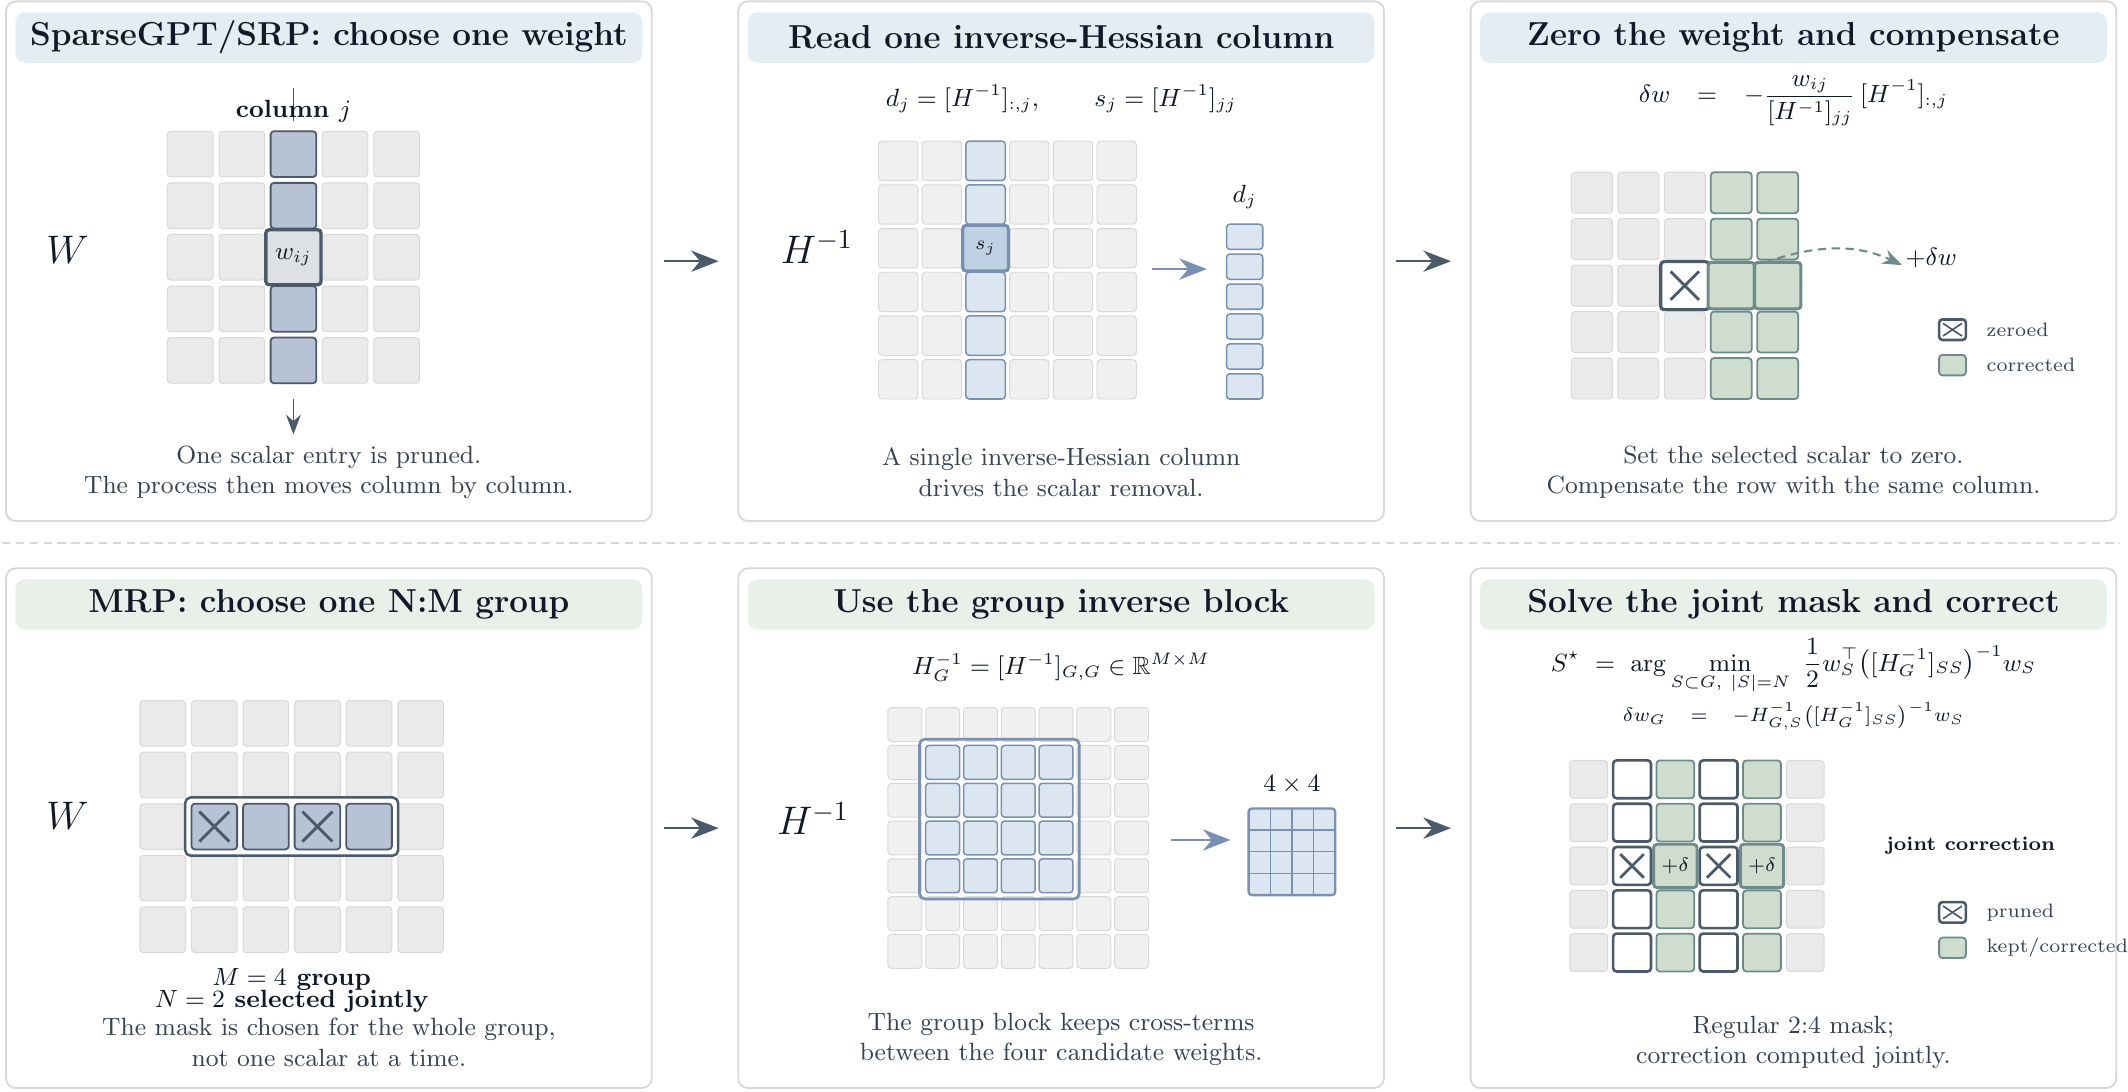
\includegraphics[width=0.8\linewidth]{figures/compression/sparsegpt_mrp_compensation.png}
\caption[Second-order compensation strategies for unstructured and semi-structured pruning.]{Second-order compensation strategies for unstructured and semi-structured pruning.}
\label{fig:hessian_compensation}
\end{figure}

\methodsep

\subsection{Fisher-Based Post-Training Structured Pruning}

The post-training framework of Kwon et al. \cite{kwon2022fast} applies second-order structured pruning without end-to-end post-pruning weight optimization. Binary masks over attention heads and FFN filters are found by solving
\begin{equation}
	\arg\min_{\mathbf{m}} \mathcal{L}(\mathbf{m})
	\quad \text{s.t.} \quad
	\mathrm{Cost}(\mathbf{m}) \leq C,
\end{equation}
where $\mathrm{Cost}$ is either a FLOPs or measured latency budget. Expanding around the dense mask and applying a diagonal Fisher approximation reduces the search to selecting units with the smallest diagonal Fisher scores subject to the cost constraint. For latency-constrained pruning, a piecewise-linear lookup table replaces the analytical cost model to incorporate real device behavior:
\begin{equation}
	\mathrm{LAT}(\mathbf{m}_{\ell}) =
	\begin{cases}
		0, & \|\mathbf{m}_{\ell}\|_0 = 0, \\
		c, & 0 < \|\mathbf{m}_{\ell}\|_0 \leq T, \\
		a(\|\mathbf{m}_{\ell}\|_0 - T) + c, & \|\mathbf{m}_{\ell}\|_0 > T,
	\end{cases}
\end{equation}
Where $c$ represents the base latency for any non-empty layer settings, $T$ denotes the structural threshold below which the latency remains relatively constant, and $a$ is the slope describing how measured latency increases beyond $T$. The lookup table is accessed when searching for the mask to get an estimate for the latency of each pruned MHA or FFN layer on the target device, enabling the selection of a mask that fulfills a measured latency budget.

\methoddetail{Algorithm Overview}
The method proceeds in four steps: (1) diagonal Fisher scores are computed for head and FFN-filter masks on a small calibration set (2K training examples); (2) a FLOPs- or latency-constrained mask search is solved under the diagonal Fisher objective; (3) a block-diagonal Fisher refinement is applied layer by layer to recover interactions ignored by the diagonal approximation; (4) surviving mask values are tuned by layer-wise linear least-squares reconstruction. Because only mask values are updated, the method avoids end-to-end weight retraining. The paper reports pruning times of 39 seconds on GLUE and 135 seconds on SQuAD, compared to 33 hours for CoFi on MNLI.

\methodsep

\subsection{Inference-Aware Structured Second-Order Pruning (ZipLM)}

ZipLM\cite{kurtic2023ziplm} extends the OBS-style reconstruction objective from individual weights to executable Transformer structures. The pruned objects are attention heads, FFN intermediate channels, and, at the coarser level, entire residual modules such as the attention block or the FFN block. For a candidate structure $S$ with column mask $\mathbf{M}_S$, the removal score is
\begin{equation}
	\arg\min_S
	\sum_{i=1}^{d_{\text{row}}}
	\mathbf{W}_{i,\mathbf{M}_S}
	\left(\left(\mathbf{H}^{-1}\right)_{\mathbf{M}_S,\mathbf{M}_S}\right)^{-1}
	\mathbf{W}_{i,\mathbf{M}_S}^{T},
\end{equation}
where $d_{\text{row}}$ is the output dimension of the weight matrix and the sum aggregates the reconstruction cost across all output rows. After removing a structure, the exact compensation and Hessian update are applied through block Gaussian elimination, so that all subsequent saliency scores remain consistent with the already-pruned state.

\methoddetail{Inference-Aware Search}
ZipLM adds a device-level objective on top of the local second-order scoring. It benchmarks attention and FFN configurations on the target hardware and stores measured runtimes in a lookup table. The global search then minimizes layer-wise structural sensitivity subject to a real speed constraint $\sum_\ell \tau_{\ell,s_\ell} \leq T_{\text{target}}$.

\methoddetail{Algorithm Overview}
ZipLM follows an iterative pruning-and-recovery regime in the sense of Section~\ref{subsec:iterative_pruning}: pruning steps are interleaved with fine-tuning rounds. It operates in two phases (see Figure~\ref{fig:ziplm_pipeline}). In the global phase, attention-head and FFN configurations are benchmarked on the target environment and a layer-wise sparsity profile satisfying the speedup requirement is selected. In the local phase, each selected layer is compressed by iteratively scoring candidate structures with the structured saliency metric, applying the optimal weight compensation, and updating the inverse Hessian by block Gaussian elimination. Recovery follows a gradual prune-and-fine-tune schedule with combined task, logit, and token-level distillation losses, at a cost of 8--10 fine-tuning epochs per pruning step.

\begin{figure}[H]
	\centering
	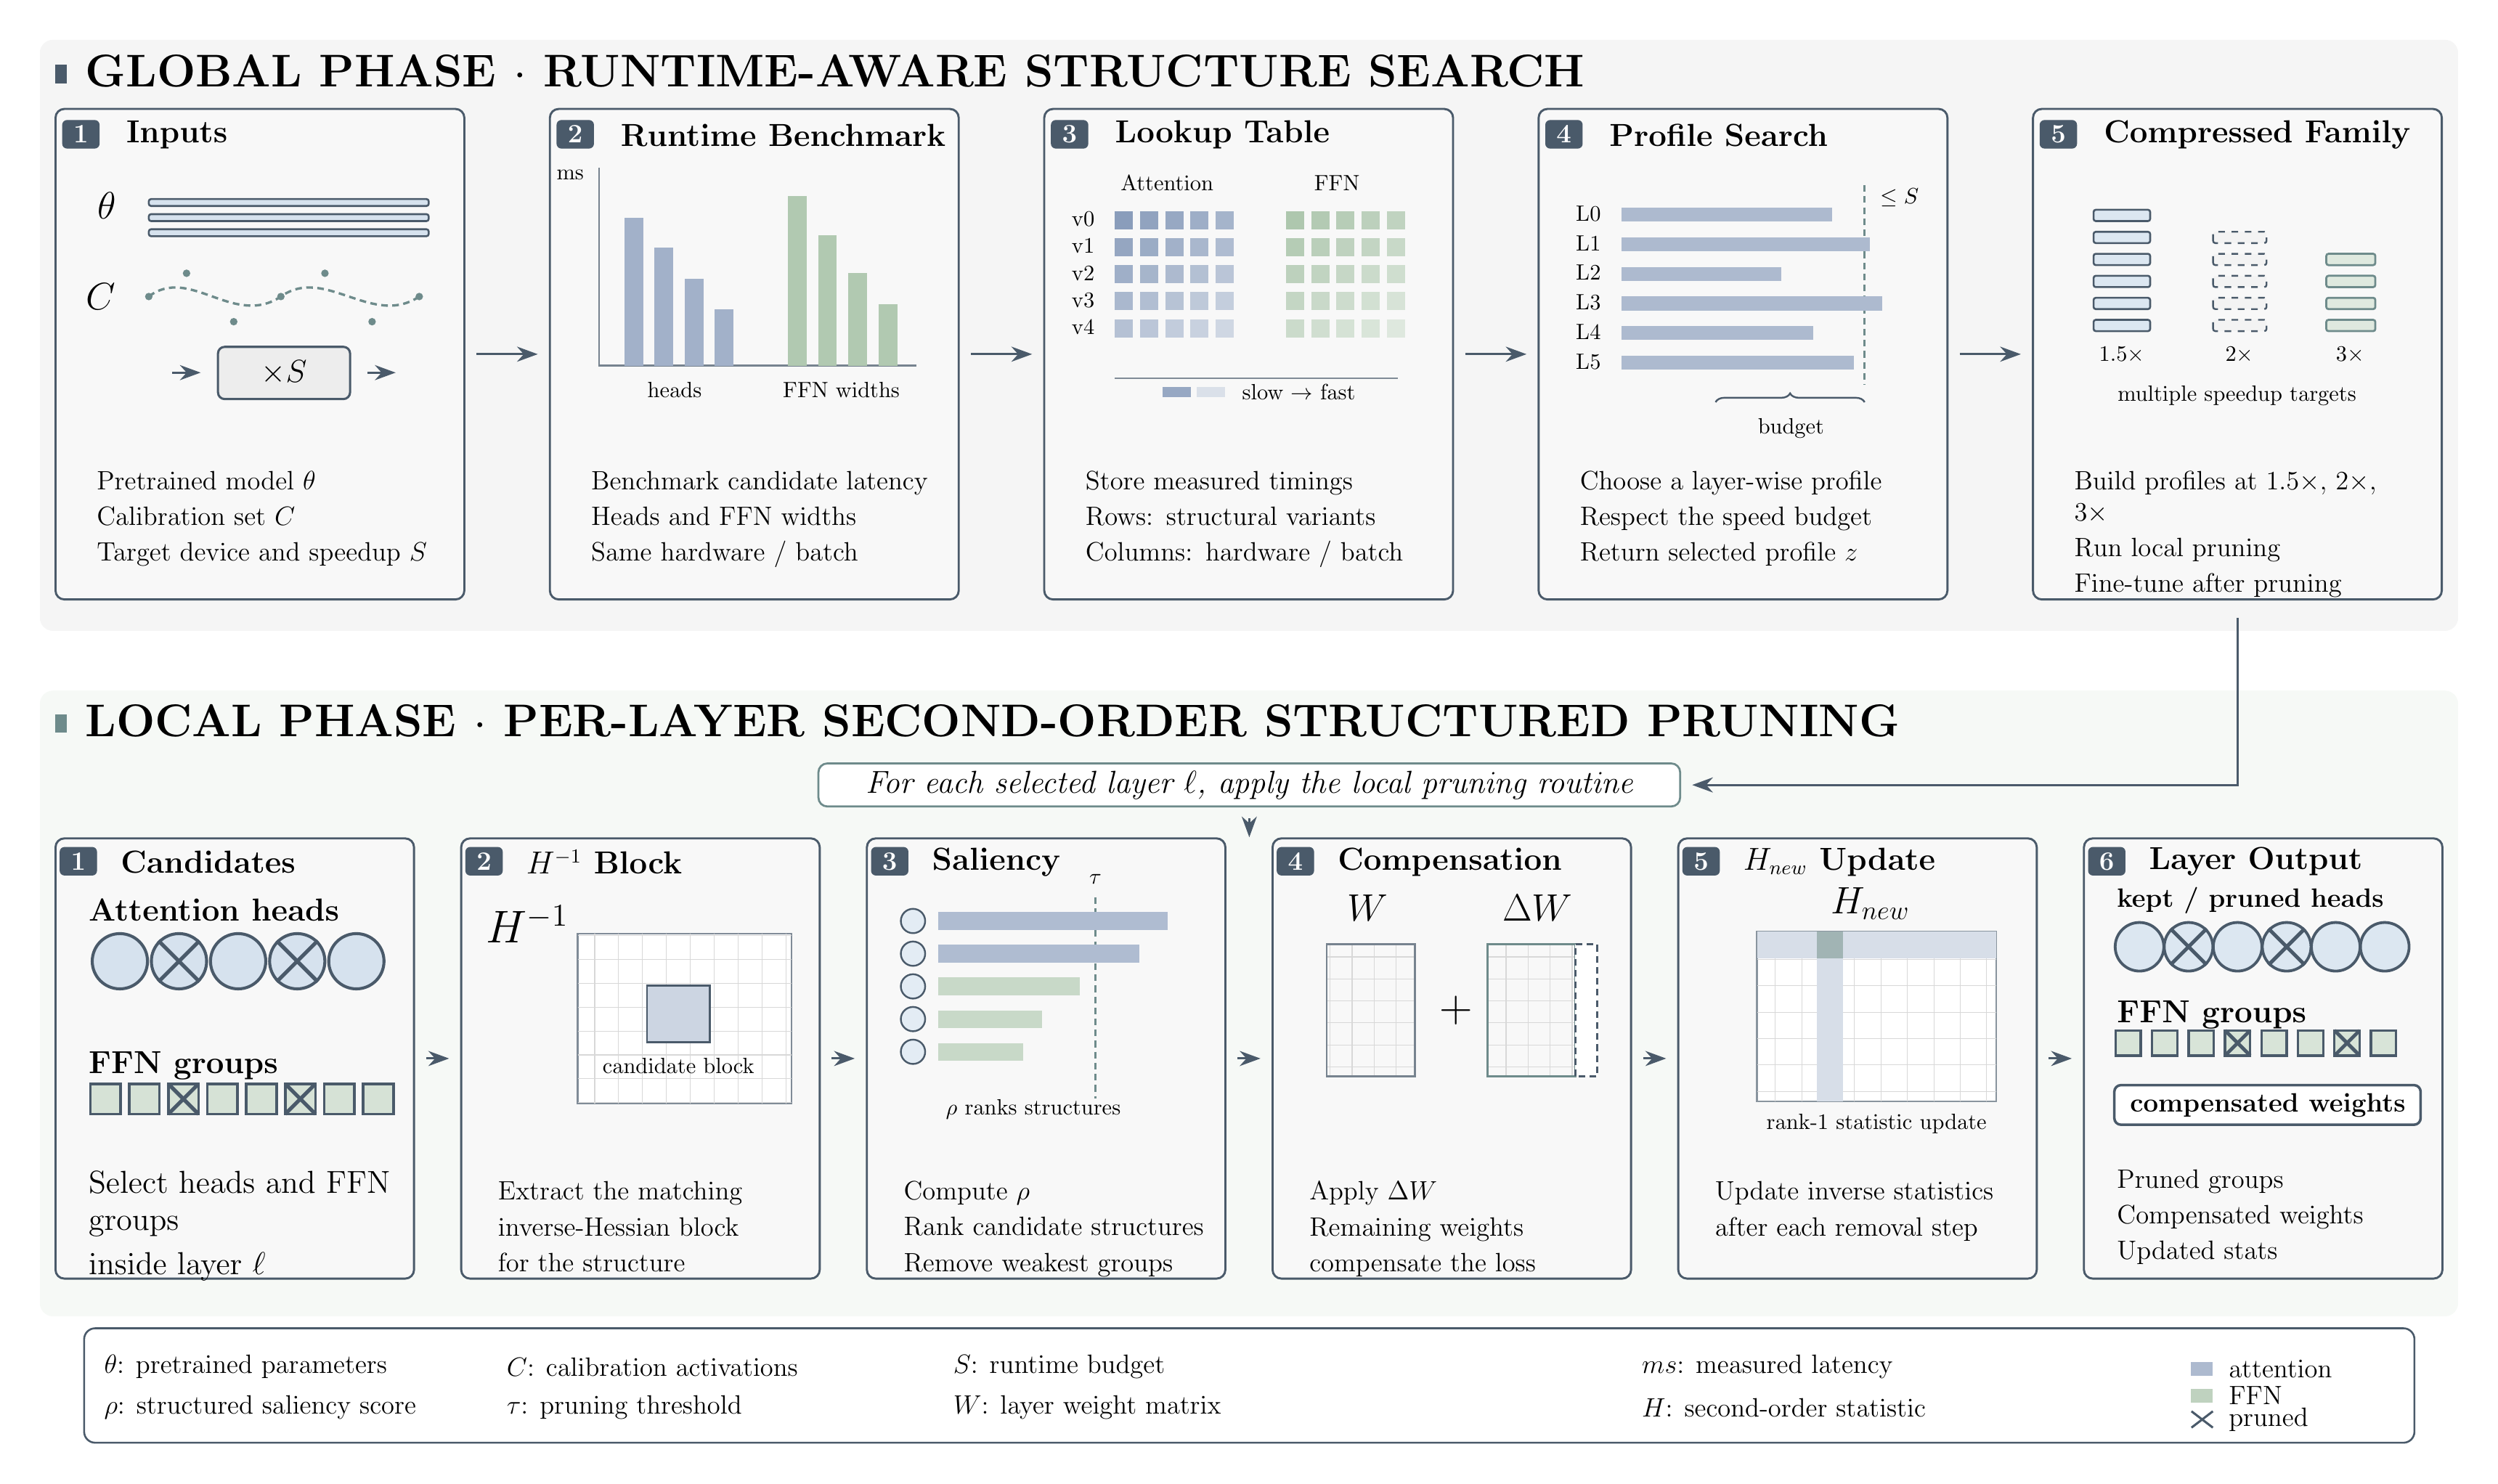
\includegraphics[width=0.96\textwidth]{figures/compression/ziplm_diagram.png}
	\caption[ZipLM pipeline.]{ZipLM pipeline. The global phase benchmarks attention-head and FFN configurations and searches for layer-wise sparsity profiles satisfying the required speedup. The local phase applies second-order structured pruning through inverse-Hessian scoring, compensation updates, and iterative Hessian refinement.}
	\label{fig:ziplm_pipeline}
\end{figure}

Second-order methods reduce local reconstruction error, but they do not fully resolve the allocation problem across the whole model. A method may know how to remove a head or channel with limited local damage and still not know how many heads or FFN channels should remain in each layer under a global budget. This is the point at which search-based methods become relevant.
\section{Conclusion}
This chapter examined structured pruning as a mechanism for generating hardware-agnostic, dense-shape acceleration. By reviewing LLM-Pruner, CoFi, Fast PTPF, and ZipLM, we illustrated how the pruning objective must adapt when removing highly coupled components like attention heads and feed-forward channels. Because structural removals are highly destructive, these methods rely on sophisticated techniques to preserve accuracy, ranging from dependency mapping to joint mask optimization and second-order Hessian compensations.

However, evaluating these methods in isolation only tells half the story. To understand the true state of Transformer compression, we must compare the structured methods discussed in this chapter with the unstructured and heterogeneous methods from Chapter 4. Therefore, the following chapter will provide a comprehensive cross-regime empirical comparison, identify the critical limitations in current evaluation protocols, and formally define the unresolved ``allocation problem'' that motivates the contribution of this thesis.



\chapter{Synthesis, Empirical Comparison, and Limitations}
\label{chap:pruning_comparison}
\section{Introduction}
The previous two chapters surveyed Transformer pruning through unstructured/heterogeneous methods (Chapter 4) and structured methods (Chapter 5). These methods optimize different units, rely on different recovery pipelines, and target different deployment metrics, so their results cannot be reduced to a single compression table. The comparison in this chapter focuses on what the evidence actually supports: where pruning remains accurate, where recovery dominates the result, and where local scoring fails to determine a strong global configuration.


\section{Empirical Comparison}
\label{subsec:empirical_comparison}

The empirical results are grouped by pruning regime because each regime reports a different kind of outcome. Unstructured and N:M methods mainly report perplexity under weight sparsity, structured methods report task accuracy or speedup after architectural removal, and search-based methods report complete pruning configurations under budget constraints.

\subsection{Unstructured and Semi-Structured Results}

Table~\ref{tab:unsupported_comparison} reports representative low, medium, and large model settings. The unstructured rows compare magnitude pruning, SparseGPT, and Wanda at 50\% sparsity, and the 2:4 rows show the semi-structured setting that motivates group-aware compensation such as MRP.

\begin{table}[H]
	\centering
	\caption[Representative unstructured and semi-structured pruning results on WikiText perplexity.]{Representative unstructured and semi-structured pruning results on WikiText perplexity. PPL denotes perplexity; lower is better.}
	\label{tab:unsupported_comparison}
	\begin{tabular}{@{}llcccc@{}}
		\toprule
		\textbf{Model} & \textbf{Setting} & \textbf{Dense PPL} & \textbf{Magnitude PPL} & \textbf{SparseGPT PPL} & \textbf{Wanda PPL} \\
		\midrule
		LLaMA-7B  & 50\% unstructured & 5.68 & 17.29 & 7.22 & 7.26 \\
		LLaMA-30B & 50\% unstructured & 4.77 & 7.54  & 5.31 & 5.24 \\
		LLaMA-65B & 50\% unstructured & 3.56 & 5.90  & 4.57 & 4.57 \\
		\midrule
		OPT-13B   & 50\% unstructured & 10.13 & $1.2{\times}10^4$ & 11.17 & -- \\
		OPT-175B  & 50\% unstructured & 8.35  & $4.3{\times}10^4$ & 8.21  & -- \\
		\midrule
		OPT-13B   & 2:4 semi-structured & 10.13 & -- & 12.96 & -- \\
		OPT-66B   & 2:4 semi-structured & 9.34  & -- & 10.09 & -- \\
		OPT-175B  & 2:4 semi-structured & 8.35  & -- & 8.74  & -- \\
		\bottomrule
	\end{tabular}
\end{table}

The results show that pure magnitude pruning can fail badly at 50\% sparsity, especially on OPT models, whereas activation-aware and second-order criteria preserve perplexity much more effectively. The 2:4 rows also show that semi-structured pruning is not just unstructured pruning with a different mask shape: the local group constraint changes the compensation problem and motivates methods such as MRP.

\subsection{Structured Pruning Results}

Table~\ref{tab:structured_summary} summarizes representative structured-pruning results across compression and speedup regimes. The table keeps the evaluation suite explicit: CoFi is reported on GLUE tasks and SQuADv1, Fast PTPF reports GLUE/SQuAD results, and ZipLM reports GLUE-style classification tasks and SQuADv1.

\begin{table}[H]
	\centering
	\caption[Representative structured Transformer pruning results across recovery regimes.]{Representative structured Transformer pruning results across recovery regimes. GLUE denotes the General Language Understanding Evaluation benchmark, SQuADv1 denotes Stanford Question Answering Dataset version 1.1, acc. denotes accuracy, and F1 denotes question-answering F1 score.}
	\label{tab:structured_summary}
	\begin{tabular}{@{}llp{4.4cm}p{4.7cm}@{}}
		\toprule
		\textbf{Method} & \textbf{Model} & \textbf{Setting} & \textbf{Key result} \\
		\midrule
		LLM-Pruner \cite{ma2023llmpruner}
		  & LLaMA-7B & 20\% prune ratio & 94.97\% zero-shot accuracy retention after LoRA recovery \\
		  & LLaMA-7B & 50\% prune ratio & 77.4\% zero-shot accuracy retention after LoRA recovery \\
		\midrule
		CoFi \cite{xia2022structured}
		  & BERT Base & GLUE/MNLI, $\approx 12{\times}$ speedup & 80.6 acc.; TinyBERT$_4$ reports 78.8 at similar speedup \\
		  & BERT Base & SQuADv1, $\approx 8.7{\times}$ speedup & 82.6 F1, matching TinyBERT$_4$ at comparable speedup \\
		\midrule
		Fast PTPF \cite{kwon2022fast}
		  & BERT Base & GLUE and SQuADv1, FLOPs-constrained pruning & 60--70\% FLOPs with $\leq 1\%$ accuracy/F1 drop \\
		  & BERT Base & GLUE and SQuADv1, latency-constrained pruning on V100 & $1.34{\times}$--$1.47{\times}$ geometric-mean speedup depending on batch size \\
		\midrule
		ZipLM \cite{kurtic2023ziplm}
		  & BERT Base & GLUE/QNLI and MNLI, $2{\times}$ speedup & 91.4 / 84.8 acc.; essentially dense-level performance \\
		  & BERT Base & GLUE/QNLI and MNLI, $10{\times}$ speedup & 88.6 / 82.7 acc.; approximately 5M parameters \\
		  & BERT Large & SQuADv1, $10{\times}$ speedup & 89.1 F1 with 20.9M parameters \\
		\bottomrule
	\end{tabular}
\end{table}

These results are closer to deployment because the methods remove executable units, but they still depend heavily on the evaluation and recovery setup. CoFi uses task-specific training, LLM-Pruner depends on LoRA recovery, Fast PTPF is largely post-training, and ZipLM adds device-specific runtime profiling. The numbers therefore show the achievable trade-offs within each protocol, not a clean ranking across methods.

\subsection{Evolutionary and Search-Based Results}

Table~\ref{tab:search_summary} reports representative search-based results for EvoPress and DarwinLM. EvoPress searches over depth-pruning and sparsity-allocation configurations, and DarwinLM uses structured evolutionary pruning with training-aware offspring selection.

\begin{table}[H]
	\centering
	\caption[Representative search-based pruning results]{Representative search-based pruning results. Wiki2 and C4 are perplexity values where lower is better; task average is accuracy where higher is better.}
	\label{tab:search_summary}
	\begin{tabular}{@{}llllccc@{}}
		\toprule
		\textbf{Setting} & \textbf{Model} & \textbf{Budget} & \textbf{Method} & \textbf{Wiki2$\downarrow$} & \textbf{C4$\downarrow$} & \textbf{Task Avg.$\uparrow$} \\
		\midrule
		Depth pruning
		  & Mistral-7B & 25\% & EvoPress & \textbf{8.66} & \textbf{12.04} & -- \\
		  & Mistral-7B & 25\% & ShortGPT & 43.26 & 40.16 & -- \\
		  & Mistral-7B & 25\% & Shortened LLaMA & 14.94 & 19.30 & -- \\
		\midrule
		Depth pruning
		  & Llama-2-7B & 37.5\% & EvoPress & \textbf{17.98} & \textbf{18.91} & -- \\
		  & Llama-2-7B & 37.5\% & ShortGPT & 70.94 & 63.51 & -- \\
		  & Llama-2-7B & 37.5\% & Shortened LLaMA & 35.37 & 26.07 & -- \\
		\midrule
		Unstructured allocation
		  & Mistral-7B & 70\% & EvoPress & \textbf{14.42} & \textbf{16.46} & \textbf{53.8} \\
		  & Mistral-7B & 70\% & OWL & 17.22 & 21.66 & 51.9 \\
		  & Mistral-7B & 70\% & Uniform & 23.08 & 30.03 & 49.9 \\
		\midrule
		Structured search
		  & Llama-2-7B & 2.7B model & DarwinLM & -- & -- & 62.8 after 10B-token post-training \\
		  & Llama-2-7B & 2.7B model & ShearedLLaMA & -- & -- & 62.6 after 50B-token post-training \\
		\bottomrule
	\end{tabular}
\end{table}

The search-based results make the allocation issue explicit. EvoPress improves over local or heuristic allocation when multiple removals interact, and DarwinLM shows that training-aware evolutionary selection can produce strong structured models with less post-training data than a fixed pruning baseline.

\subsection{Cross-Regime Synthesis}

Table~\ref{tab:pruning_empirical_summary} condenses these comparisons into the main implications for pruning-search design.

\begin{table}[H]
	\centering
	\caption{Aggregated interpretation of the empirical pruning evidence by regime.}
	\label{tab:pruning_empirical_summary}
	\begin{tabularx}{\textwidth}{@{}>{\raggedright\arraybackslash}p{2.5cm}>{\raggedright\arraybackslash}p{3.0cm}LL@{}}
		\toprule
		\textbf{Regime} & \textbf{Representative setting} & \textbf{Selected evidence} & \textbf{Reading} \\
		\midrule
		Weight-level unstructured
		& LLaMA-7B, 50\% sparsity
		& Dense PPL 5.68; magnitude 17.29; SparseGPT 7.22; Wanda 7.26.
		& Better saliency preserves perplexity, but the resulting pattern remains unstructured and does not guarantee dense-kernel speedup. \\
		\addlinespace
		Semi-structured N:M
		& OPT-13B, 2:4 sparsity
		& Dense PPL 10.13; SparseGPT-style compensation gives 12.96 under the 2:4 constraint.
		& N:M sparsity needs group-aware compensation, which motivates MRP-style joint treatment of simultaneously removed weights. \\
		\addlinespace
		Structured LLM pruning
		& LLM-Pruner on LLaMA-7B
		& 20\% prune ratio retains 98.6\% zero-shot accuracy after LoRA recovery; 50\% retains 83.6\%.
		& Dependency-aware pruning keeps the model executable, with final quality strongly tied to recovery. \\
		\addlinespace
		Structured encoder pruning
		& CoFi, Fast PTPF, and ZipLM on BERT
		& CoFi reaches 80.6 MNLI acc. near $12{\times}$ speedup; Fast PTPF keeps 60--70\% FLOPs with $\leq$1\% drop; ZipLM reaches 88.6/82.7 QNLI/MNLI acc. at $10{\times}$ speedup.
		& Structured pruning can produce executable acceleration, with protocols differing in training cost, hardware profiling, and recovery budget. \\
		\addlinespace
		Search-based pruning
		& EvoPress and DarwinLM
		& EvoPress improves depth-pruning and sparsity-allocation baselines; DarwinLM reports 62.8 average accuracy after 10B-token post-training versus 62.6 for ShearedLLaMA after 50B tokens.
		& Configuration search addresses global allocation, and training-aware selection improves structured candidates beyond one-shot scoring. \\
		\bottomrule
	\end{tabularx}
\end{table}


\begingroup
\def\RenderPruningReviewDiscussion{}
% ============================================================
%  Drop-in discussion sections, compile inside your main .tex
%  Requires: amsmath, booktabs, enumitem, hyperref, algorithm,
%            algpseudocode, multirow, tabularx, array, xcolor
% ============================================================

% =============================================================
\ifdefined\RenderPruningReviewDiscussion
\section{Discussion}
\label{sec:discussion}
% =============================================================

The distinction between the two questions has been separated between Chapters~\ref{chap:related_work_pruning_unstructured} and~\ref{chap:related_work_pruning_structured} and in the empirical comparison, Section~\ref{subsec:empirical_comparison}. One question is: for a single unit that is potentially removable, what criterion should be used to rank the units? Here, different magnitude-based, gradient-based, and curvature-based criteria offer varying estimates. The second question is: how is the overall budget of pruning shared among the units in the model? Here, the approaches tend to diverge more substantially, and much of the outstanding debate in the literature is focused on the latter. It will be discussed here, then the empirical data.

\subsection{Local Scoring Versus Global Allocation}
\label{subsec:local_vs_global}

The methods reviewed in this chapter differ in implementation, pruning unit, and recovery cost, but they can all be related to the same underlying objective:
\begin{equation}
  \min_{\mathcal{M} \in \mathcal{F}}\; \Delta\mathcal{L}(\mathcal{M}),
  \label{eq:master}
\end{equation}
where $\mathcal{M}$ denotes a feasible sparsity pattern or structured subnetwork and $\Delta\mathcal{L}$ denotes the loss increase caused by pruning. The difficulty is that $\mathcal{M}$ must satisfy a compression budget while preserving the behaviour of the model.

Another persistent issue with the pruning criteria discussed so far is their evaluation of weights and activations, which can be removed before the final compressed model is fixed. SparseGPT calculates approximate second-order local reconstruction costs of sets of weights \cite{frantar2023sparsegpt}, while Wanda sorts parameters by a product of weight magnitude and input activation norm \cite{sun2023simple}. These methods are successful in finding some locally removable weights but fail to determine the overall distribution of compression under a fixed budget across the layers \cite{hoefler2021sparsity,cheng2024pruningsurvey}. Though one-shot local pruning works well under low compression ratios, high compression rates require more sophisticated iterative and global-allocation-based pruning methods \cite{janusz2025oneshot}. Several of these recent methods implicitly or explicitly address this issue: ZipLM attempts to find explicit local and global correlations between layers, and EvoPress directly searches over the layer-wise compression budgets that minimize the distribution divergence of the output \cite{kurtic2023ziplm,evopress2024}.

\subsection{Limitations of Local Ranking at High Compression}
\label{subsec:inadequacy}

In the analyses above, we can observe one trend across these method families. It appears that local ranking criteria are successful when the compression ratio is relatively small to medium; when the targeted compression ratio becomes higher, the deficiencies of local ranking criteria tend to become apparent \cite{hoefler2021sparsity,sanh2020movement,bai2024sparsellm,janusz2025oneshot}. This pattern is expected from the definition of the pruning problem: local criteria judge removeable units while the ultimate compressed model has not been formed completely.

For Transformer models, structured pruning is naturally expressed as a layer-wise allocation problem over executable units. A pruned Transformer may retain different numbers of attention heads, FFN intermediate dimensions, hidden dimensions, or even complete MHA/FFN modules in different layers \cite{xia2022structured,kurtic2023ziplm,cheng2024pruningsurvey}. Thus, for a model with $L$ layers, $H$ attention heads per layer, and $F$ FFN channels per layer, the retained structure can be represented by an allocation vector
\[
  \mathbf{s} = (h_1, f_1, h_2, f_2, \ldots, h_L, f_L),
\]
subject to a global MAC budget $\Omega$. Recent layer-wise pruning work therefore treats compression as the problem of assigning adaptive sparsity ratios across layers which is just a specific case of non uniform pruning \cite{li2024dsa}.

Local ranking simply assigns each prunable unit a saliency and prunes the lowest ones until the budget is exhausted. it implicitly models global ranking with the assumption that each pruning decision can be made in isolation. EvoPress recognizes this assumption in the domain of depth pruning; block-scoring algorithms use the assumption that error is linear such that each block is thought to contribute equally to the overall compression error \cite{evopress2024}. ZipLM takes the reverse argument, stating that pruning has to capture both within layer local correlations and across layer global correlations \cite{kurtic2023ziplm}.

The compositional structure of the Transformer violates the independence approximation. Each Transformer block comprises the residual-connected attention and feed-forward sublayers and self-attention layers take representations as input which are generated from previous layers \cite{vaswani2017attention}. With regard to pruning, this indicates that any alteration on one layer will bring new input distribution for the following layers. SparseLLM is the first one who precisely identifies the problem by modeling an LLM as a chain of modules, where outputs of a module become the inputs for another, and points out that local layer error reduction only causes non-optimal performance for the global pruning at a high sparsity rate \cite{bai2024sparsellm}.

The same coupling is present for attention and the global budget constraint. Scaled dot-product attention normalizes the query-key score using a softmax, while multi-head attention merges multiple heads which act on the same input layer \cite{vaswani2017attention}. Experimentally, attention heads can have unequal importance, numerous can be dropped, beyond a threshold, attention collapses catastrophically, and different components of the attention function can have differing sensitivity \cite{michel2022not}. In addition, if the MAC budget is fixed, having high capacity in one layer means we must sacrifice capacity elsewhere. Prior works have indicated the necessity of across-layer uneven sparsity under high compression \cite{gale2019state,sanh2020movement,li2024dsa}.

% =============================================================
\section{Empirical Results}
\label{sec:empirical}
% =============================================================

Having argued that allocation is more important than local scoring at high compression, the question is whether the results reflect this. On the whole, they do but only if we treat apples and oranges distinctly. The results on the unstructured model isolate the saliency rule in the absence of weight sparsity and the structured/search based readings bring back the cost of recovery and the budget allocation aspect.

\subsection{Unstructured and Semi-Structured Methods}
\label{subsec:unstructured_results}

The unstructured pruning results allow three clean comparisons across increasing levels of local sophistication: magnitude baseline, Wanda (activation-aware saliency), and SparseGPT (second-order compensation).

The SparseGPT results primarily highlight the instability of pure magnitude pruning at high sparsity. At 50\% sparsity on OPT-13B, magnitude pruning produces a perplexity of $1.2\times10^4$ compared to the dense model's 10.13. This indicates severe representational degradation under weight selection based solely on individual magnitude. SparseGPT reduces the same setting to 11.17, corresponding to a $+1.04$ increase over the dense model.

The comparison between Wanda and SparseGPT on LLaMA models is also instructive. At 50\% sparsity on LLaMA-7B, Wanda achieves 7.26 versus SparseGPT's 7.22, a negligible 0.04 point difference. On LLaMA-13B, Wanda actually outperforms SparseGPT by 0.06 points (6.15 versus 6.21). This apparent paradox reflects two facts. First, the Wanda activation norm $\|x_j\|_2$ is an effective proxy for the weight's contribution to the output, particularly in models with large activation outliers, which LLaMA models exhibit. Second, the calibration set used for Hessian construction in SparseGPT introduces variance that at moderate sparsity levels can offset the theoretical advantage of curvature information. At higher sparsity levels (70\%+), the second-order advantage of SparseGPT becomes more consistent, because local reconstruction errors accumulate and the precise compensation direction matters more.

\subsection{Structured Methods}
\label{subsec:structured_results_discussion}

Both CoFi and ZipLM obtain similar accuracy at similar speedups but employ very different preparation pipeline. CoFi obtains 80.6 on MNLI with about $12\times$ speedups after 20 hours of combined mask and weight optimization, whereas ZipLM gets 81.7 at $35\times$ through scheduled fine-tuning interspersed with structured pruning stages and dedicated hardware benchmarking. Here the accuracies represent the accuracy of the whole pipeline not only the pruning criterion, because the recovery approaches they employ differ greatly and thus the two methods are not directly comparable.

\subsection{Cross-Method Comparison}
\label{subsec:cross_method}

The tables above support two conclusions. At 50\% unstructured sparsity on OPT-13B, magnitude pruning collapses to a perplexity of $1.2\times10^4$ while SparseGPT reaches 11.17 (Table~\ref{tab:unsupported_comparison}), showing that second-order compensation is necessary once individual weight interactions become non-negligible. At 70\% unstructured sparsity on Mistral-7B, EvoPress reaches 14.42 perplexity while uniform allocation reaches 23.08 (Table~\ref{tab:search_summary}), and at 37.5\% depth sparsity on Llama-2-7B, EvoPress gives 17.98 against ShortGPT's 70.94, showing that global allocation search becomes the dominant factor at high compression.

\section{Limitations of the Reviewed Methods}
\label{sec:limitations}

 The observations above suggest genuine differences between the methods. However, most of the disparity observed is can simply be a reflection of how each paper was evaluated. There are three consistent issues which have affected nearly every cross-paper assertion: unequal testing scenarios, disparate recovery budget sizes and sensitivity to a calibration set whose effect is usually not examined.

\subsection{Evaluation Protocol Heterogeneity}
\label{subsec:eval_protocol}

A significant drawback in the pruning literature is the lack of a universal evaluation protocol. Approaches are presented under five, and possibly more, different evaluation schemes. The first reports language model perplexity under fixed nominal sparsity, while the second measures zero-shot task performance accuracy with or without recovery. The third instead reports supervised fine-tuning performance accuracy with or without recovery, whereas the fourth measures actual wall-clock speedup or latency given particular hardware. Finally, the fifth reports FLOPs reduction compared to the dense model.

These five schemes are incommensurable. A method presenting $99\%$ dense accuracy after $2\times$ FLOPs reduction addresses a different evaluation goal compared to another method presenting $1.5\times$ wall-clock speedup at a $<1\%$ accuracy drop. FLOPs is a hardware-agnostic theoretical metric that does not necessarily linearly translate to wall-clock runtime, which depends on memory bandwidth, batch size, and the particular accelerator execution model. Certain sparse execution formats require hardware support, while the simple unstructured masks often do not result in a proportional wall-clock speedup over standard dense kernels.

The fragmentation of evaluation makes it difficult to compare across papers. If a table presents Wanda~\cite{sun2023simple}, CoFi~\cite{xia2022structured}, LLM-Pruner~\cite{ma2023llmpruner}, ZipLM~\cite{kurtic2023ziplm}, and EvoPress~\cite{evopress2024} in the same rows, one implicitly assumes that they all aim to solve the same problem. In reality, each method targets different budgets, recovery schemes, and deployment targets. When summarized without qualification, the methods present a false picture of one single Pareto frontier.

\subsection{Recovery Budget Inconsistency}
\label{subsec:recovery}

Relatedly is the issue of different recovery budgets. It's expected that structured pruning results in a larger loss in accuracy than unstructured pruning for a given sparsity, making the recovery stage particularly important \cite{xu2026lightweight}. The difference in terminology of ``post-training pruning'' versus ``pruning with fine-tuning'' in reality represents a wide range of recovery costs that contribute to reported accuracy. Among the methods in the above literature, Fisher post-training pruning only tunings the masks with zero weight updates and total tuning time about 39 sec. LLM-Pruner tunings using 2.5 hrs of LoRA recovery on 50k examples with rank 8 adapter. ZipLM tunes over 8-10 epochs per pruning steps with the whole model fine-tuning and full distillation. CoFi joint tunes mask and weights in 40 epochs with a task specific teacher model.

An appropriate comparison needs to keep recovery budgets constant. The model of 40 epochs fine-tuning for CoFi should not be compared to LLM-Pruner's 2.5 hrs of LoRA recovery. Given the same budget, the gap would be much smaller. Very few articles performed such fair comparisons, and thus, some accuracy differences we see in the literature should be attributed to the amount of recovery budget.

\subsection{Calibration Set Sensitivity}
\label{subsec:calibration}

All post-training pruning techniques rely on a calibration set in order to compute either saliency scores, Hessian surrogates, or Fisher information matrices. The specific selection of the calibration set results in differences in the resulting pruned model which are usually not explored in a principled way.

For language models, it is a common practice to use 128–2048 examples from a general language corpus like C4 or WikiText. This is a small fraction of the model’s training distribution, and may not be representative of activation statistics used to determine saliency. LLM-Pruner calibrates using 10 short examples, which is dramatically fewer than SparseGPT's 128 examples and may contribute to variance in its Taylor scores, and consequently in its reported zero-shot accuracies across trials. More generally, all methods employing a calibration set make the implicit assumption that a ranking based on calibration examples transfers to the whole evaluation distribution. It has recently been shown that the calibration set is extremely important in post-training pruning, especially for high sparsity rates, and that pruning works better with calibration data that matches the pre-training distribution \cite{ji2025calibration,bandari2024calibration}.{ji2025calibration,bandari2024calibration}.

% =============================================================
\fi
\ifdefined\RenderProposedPruningSearchFramework
\chapter{Proposed Pruning-Search Framework}
\label{sec:design}
\label{chap:proposed_pruning_search_framework}
% =============================================================

\section{Design Philosophy and Motivation}
\label{subsec:design_philosophy}

The design of the proposed framework follows directly from the gaps identified in Sections~\ref{sec:discussion}--\ref{sec:limitations}. The central premise is that structured pruning at moderate-to-high compression rates is a combinatorial optimisation problem over architectural configurations. The main methodological deficiency in the reviewed methods lies in global allocation strategy rather than in local saliency estimation alone. The pruning-search paper addresses this point explicitly by treating head retention, FFN width, and active depth as a joint discrete decision and by organising the search around feasibility, representation fidelity, and diversity preservation.

Three design principles follow from this premise.
z
\medskip\noindent\textbf{Principle 1: The configuration is the primary optimisation object.} The framework treats the allocation vector $\mathcal{C} = (\mathbf{h}, \mathbf{n})$ as the optimisation variable. Every operation is defined on complete configurations rather than on per-unit scores. This allows direct evaluation of the joint effect of all removals and keeps the budget constraint explicit throughout the search.

\medskip\noindent\textbf{Principle 2: The feasible set is explicitly enforced.} Rather than soft-penalising infeasible configurations, the framework enforces the MAC constraint and minimum active-depth requirement through a repair projection that maps every mutated configuration back into $\mathcal{F}$ before fitness evaluation. This guarantees that every evaluation corresponds to a deployable architecture.

\medskip\noindent\textbf{Principle 3: Diversity is as important as fitness.} Because the configuration space contains many local optima that are structurally distant from each other, a search that maximises raw fitness without diversity control will converge to one architectural type and miss better solutions elsewhere. The framework therefore maintains diversity explicitly through shared-fitness selection, MAP-Elites archiving, and Pareto preservation.

\section{Configuration Space Formalisation}
\label{subsec:config_space}

The pruning-search paper formalises the search variable as a joint head-and-neuron configuration. For a Transformer with $L$ layers and $H$ heads per layer, the candidate is
\begin{equation}
  \mathcal{C} = (\mathbf{h}, \mathbf{n}), \qquad
  \mathbf{h} \in \{0,1\}^{L \times H}, \quad
  \mathbf{n} \in \beta \mathbb{Z}_{\ge 0}^{L},
  \label{eq:design_candidate}
\end{equation}
where $h_{\ell,k}=1$ indicates that head $k$ of layer $\ell$ is retained and $n_\ell$ is the retained FFN width in multiples of a hardware-aligned block size $\beta$.

Let $S$ denote the sequence length, $d$ the hidden dimension, and $d_h=d/H$ the head dimension. The paper uses a direct MAC accounting model in which one retained head contributes
\begin{equation}
  c_h = 4Sd_hd,
  \qquad
  c_n = 2Sd
  \label{eq:design_mac_unit}
\end{equation}
per retained FFN neuron block. The total cost is therefore
\begin{equation}
  \mathrm{MAC}(\mathcal{C})
  = \sum_{\ell=1}^{L}
  \Bigl(
    \sum_{k=1}^{H} h_{\ell,k} c_h + n_\ell c_n
  \Bigr),
  \label{eq:design_mac}
\end{equation}
and the active depth is
\begin{equation}
  K(\mathcal{C})
  =
  \#\Bigl\{
    \ell : \sum_{k=1}^{H} h_{\ell,k}>0 \text{ and } n_\ell>0
  \Bigr\}.
  \label{eq:design_active_depth}
\end{equation}
The feasible set is
\begin{equation}
  \mathcal{F}
  =
  \Bigl\{
    \mathcal{C} : \mathrm{MAC}(\mathcal{C}) \leq \Omega,\; K(\mathcal{C}) \geq K_{\min}
  \Bigr\},
  \label{eq:design_feasible}
\end{equation}
which makes the resource constraint explicit at the level of the optimisation problem itself. This is a stronger design choice than targeting nominal sparsity, because the optimisation is posed directly in the computational budget space that governs deployment.

\section{Distillation Objective and Representation Signals}
\label{subsec:fitness_design}

The paper's fitness compares student and teacher representations at several levels of the masked computation graph. For each layer $l$, three signal families are recorded:
\begin{equation}
  \Delta^{(l)} = H^{(l)} - H^{(l-1)},
  \qquad
  A^{(l)},
  \qquad
  F^{(l)},
  \label{eq:design_signals}
\end{equation}
where $\Delta^{(l)}$ is the residual hidden-state update, $A^{(l)}$ is the attention branch, and $F^{(l)}$ is the FFN branch. This is a significant design choice because structured pruning modifies intermediate computation directly, not only the final hidden state.

For student and teacher tensors $\mathbf{X},\mathbf{Y}\in\mathbb{R}^{N\times d}$, the paper defines a blended distance
\begin{align}
  d_{\mathrm{cos}}(\mathbf{X},\mathbf{Y})
  &=
  1-\frac{1}{N}\sum_{i=1}^{N}
  \frac{\mathbf{x}_i^\top \mathbf{y}_i}{\|\mathbf{x}_i\|_2\|\mathbf{y}_i\|_2},
  \label{eq:design_dcos} \\
  d_{\mathrm{mag}}(\mathbf{X},\mathbf{Y})
  &=
  \frac{\|\mathbf{X}-\mathbf{Y}\|_F^2}
       {\tfrac12(\|\mathbf{X}\|_F^2+\|\mathbf{Y}\|_F^2)+\varepsilon},
  \label{eq:design_dmag} \\
  d_{\alpha}(\mathbf{X},\mathbf{Y})
  &=
  (1-\alpha)d_{\mathrm{cos}}(\mathbf{X},\mathbf{Y})
  + \alpha d_{\mathrm{mag}}(\mathbf{X},\mathbf{Y}),
  \qquad \alpha=0.35.
  \label{eq:design_dalpha}
\end{align}
The cosine term preserves directional agreement, while the magnitude term prevents norm collapse. This detail is empirically justified in the ablation study, where removing the magnitude component lowers SST-2 accuracy by $0.5$ points.

If $\mathcal{M}_l\subseteq\{\Delta,A,F\}$ denotes the set of available signals in layer $l$, the per-layer discrepancy is
\begin{equation}
  d_l(\mathcal{C})
  =
  \frac{1}{|\mathcal{M}_l|}
  \sum_{m\in\mathcal{M}_l}
  d_{\alpha}\!\bigl(\mathbf{S}^{(l,m)}_s,\mathbf{S}^{(l,m)}_t\bigr),
  \label{eq:design_dl}
\end{equation}
and the depth term is an importance-weighted aggregation,
\begin{equation}
  d_{\mathrm{deep}}(\mathcal{C})
  =
  \sum_{l=1}^{L}\bar{w}_l d_l(\mathcal{C}),
  \qquad
  \bar{w}_l
  =
  \frac{w_l \mathbf{1}[d_l \text{ available}]}
       {\sum_j w_j \mathbf{1}[d_j \text{ available}]},
  \label{eq:design_ddeep}
\end{equation}
where $w_l$ are normalised layer-importance weights. The paper reports a $0.7$ point SST-2 drop when this depth term is removed, which is direct evidence that intermediate supervision materially improves configuration ranking.

The fitness also includes a capacity-cliff penalty for abrupt FFN bottlenecks:
\begin{equation}
  P_{\mathrm{cliff}}(\mathcal{C})
  =
  \kappa\sum_{l=1}^{L-1}
  \Bigl[
    \frac{n_l-n_{l+1}}{n_{\max}}-\delta
  \Bigr]_+
  +
  \rho\,\mathbf{1}\!\Bigl[\frac{n_L}{n_{\max}}<\eta\Bigr],
  \label{eq:design_cliff}
\end{equation}
with $\kappa=2$, $\delta=0.25$, $\rho=0.5$, and $\eta=0.10$ in the paper. This term directly targets the bottleneck collapse discussed earlier, and its removal causes an additional $0.6$ point drop in the ablation study.

The final distance is
\begin{equation}
  d(\mathcal{C})
  =
  \gamma\, d_{\mathrm{cos}}\!\bigl(H_s^{(L)},H_t^{(L)}\bigr)
  + (1-\gamma)d_{\mathrm{deep}}(\mathcal{C})
  + P_{\mathrm{cliff}}(\mathcal{C}),
  \qquad \gamma = 0.35.
  \label{eq:design_fitness}
\end{equation}
This objective is substantially richer than local saliency scoring. It is the main mechanism by which the search converts a combinatorial pruning problem into a measurable representation-fidelity problem.

\section{Proxy Selection and Structure-Aware Initialisation}
\label{subsec:initialisation}

The initialisation stage is structured rather than random. The paper defines eleven training-free proxy metrics and selects a low-correlation subset instead of using the full set indiscriminately.

If $\Phi\in\mathbb{R}^{N_s\times 11}$ denotes the proxy matrix over $N_s=60$ sampled candidates, proxy $j$ receives a uniqueness score
\begin{equation}
  u_j
  =
  \frac{\bigl|\{\phi_j^{(1)},\ldots,\phi_j^{(N_s)}\}\bigr|}{N_s},
  \label{eq:design_proxy_uniqueness}
\end{equation}
and the selected subset $\mathcal{S}$ is built greedily by balancing uniqueness against pairwise correlation:
\begin{equation}
  j^*
  =
  \arg\max_{j\notin \mathcal{S}}
  u_j
  \Bigl(
    1-\max_{k\in\mathcal{S}}|\hat r_{jk}|
  \Bigr).
  \label{eq:design_proxy_select}
\end{equation}
This selection procedure ensures that the seed population reflects genuinely different notions of importance rather than near-duplicate rankings.

The sweep varies four structural axes: the active-layer count, the layer-selection pattern, the budget-shape profile across depth, and the attention-budget fraction. In the paper, the head-budget ratio is swept over $\rho_h\in\{0.25,0.40,0.55,0.70\}$, and each affordable active-depth value receives an equal quota of candidate seeds. The initial population is therefore distributed across multiple structural regimes instead of being concentrated around a single local ranking heuristic.

The ablation study confirms that this component is important. Replacing the proxy-guided sweep with random initialisation lowers SST-2 accuracy by $1.1$ points, which is the largest single ablation drop among the search-control components.

\section{Feasible Mutation and Repair}
\label{subsec:mutation}

The search does not rely on one or two generic mutations. The paper defines a sixteen-operator vocabulary split into micro operators and macro operators.

\medskip\noindent\textbf{Micro operators.} These are local, approximately budget-neutral edits such as head swap, neuron swap, head-for-neurons trade, neurons-for-head trade, Lamarckian greedy head refinement, sparsity shift, neuron rebalance, equilibrium mutation, and low-probability jitter. Their role is local exploitation within an already promising structural region.

\medskip\noindent\textbf{Macro operators.} These are larger structural edits such as layer drop, layer activation, multi-drop, head-neuron trade, macro budget shift, group reallocate, and layer rewire. Their role is exploration across different active-depth patterns and head-neuron allocations.

\medskip\noindent\textbf{Crossover.} The operator set is complemented by three crossover modes: topology-budget crossover, group-swap crossover at a layer cut, and layerwise inheritance. This is relevant because it allows the search to recombine high-performing depth patterns with high-performing budget shapes.

After mutation or crossover, the candidate is passed through a repair operator. Let $\mathcal{L}_{\mathrm{prot}}$ denote the set of the $K_{\min}$ most important layers. The repair step first ensures that each protected layer retains at least one head and one FFN block, then enforces global head-count bounds, and finally trims excess cost until the budget is satisfied. In the paper, trimming proceeds greedily by removing one $\beta$-block from the widest layer with probability $0.6$, otherwise removing the lowest-scored active head from the densest layer, and only deactivating an unprotected layer if finer adjustments are no longer available.

At the conceptual level,
\begin{equation}
  \mathcal{C}' \leftarrow \mathrm{Repair}(\widetilde{\mathcal{C}}),
  \label{eq:design_repair}
\end{equation}
and the paper proves finite-step termination under a mild feasibility condition on the protected core. Feasibility is therefore guaranteed by construction rather than encouraged indirectly through penalty terms.

\section{Adaptive Operator Selection with EXP3-IX}
\label{subsec:exp3}

The paper does not fix operator frequencies by hand. It uses EXP3-IX to adapt operator probabilities online, which is appropriate because different operators are useful in different regions of the search space and at different stages of stagnation.

The probability of selecting operator $k$ at iteration $t$ is
\begin{equation}
  p_k(t) = (1-\gamma)\frac{w_k(t)}{\sum_{j=1}^K w_j(t)} + \frac{\gamma}{K},
  \qquad \gamma = 0.07,
  \label{eq:exp3_prob}
\end{equation}
and the weights are updated according to
\begin{equation}
  w_k(t+1) = w_k(t) \cdot \exp\!\left(\frac{\gamma \hat{r}_k(t)}{K}\right),
  \label{eq:exp3_update}
\end{equation}
with the implicit-exploration estimator
\begin{equation}
  \hat{r}_k(t) = \frac{r_k(t)\,\mathbf{1}[k_t = k]}{p_k(t) + \gamma},
  \label{eq:exp3_reward}
\end{equation}
where the paper's reward blends local and global progress:
\begin{equation}
  r(t)=0.85\,r_{\mathrm{local}}(t)+0.15\,r_{\mathrm{global}}(t).
  \label{eq:design_reward_blend}
\end{equation}
This reward is more informative than parent-child improvement alone because it also credits operators that generate globally competitive candidates. The method further refines operator selection through a niche descriptor
\begin{equation}
  \psi(\mathcal{C})
  =
  \bigl(K(\mathcal{C}),\mathrm{mac\_bucket}(\mathcal{C}),\mathrm{shape\_bucket}(\mathcal{C})\bigr),
  \label{eq:design_niche_descriptor}
\end{equation}
and a niche-conditioned sampling rule
\begin{equation}
  \tilde p_k(\psi,t)\propto p_k(t)\bigl(0.5+q_{k,\psi}(t)\bigr),
  \label{eq:design_niche_sampling}
\end{equation}
so operator effectiveness is learned both globally and within structurally similar regions of the search space.

\section{Screening and Diversity Maintenance}
\label{subsec:diversity}

The paper combines cost control and diversity control. Cost control is achieved through a two-stage evaluation protocol: every offspring receives a cheap screening pass, while only a small, diversity-aware subset is promoted to full evaluation. This reduces full-token evaluations by about 85\% with less than 0.3\% quality loss on BERT-base.

To prevent premature convergence, the raw fitness is also modified by a structural sharing penalty. The distance between two configurations $\mathcal{C}^{(a)}$ and $\mathcal{C}^{(b)}$ is defined as
\begin{equation}
  \Delta(\mathcal{C}^{(a)}, \mathcal{C}^{(b)})
  = \frac{|\mathbf{h}^{(a)} \oplus \mathbf{h}^{(b)}|_0}{2LH}
  + \frac{\sum_{\ell=1}^L |n^{(a)}_\ell - n^{(b)}_\ell|}{2L(\max_\ell\max(n_\ell^{(a)},n_\ell^{(b)})+1)},
  \label{eq:distance}
\end{equation}
which combines head-mask edit distance and FFN-width deviation. The shared fitness is
\begin{equation}
  \tilde{d}(\mathcal{C}^{(i)})
  = d(\mathcal{C}^{(i)}) \cdot
  \sum_{j=1}^{|\mathcal{P}|}
  \max\!\left(0, 1 - \frac{\Delta(\mathcal{C}^{(i)}, \mathcal{C}^{(j)})}{\sigma_{\mathrm{share}}}\right),
  \label{eq:shared_fitness}
\end{equation}
Configurations structurally similar to many others have their fitness penalised, encouraging the search to maintain coverage of the configuration space.

A MAP-Elites archive complements fitness sharing by explicitly maintaining the best configuration found for each bin of a two-dimensional behavioural space $(K(\mathcal{C}), R_{\mathrm{hn}}(\mathcal{C}))$, where
\begin{equation}
  R_{\mathrm{hn}}(\mathcal{C})
  = \frac{\sum_\ell \sum_k h_{\ell,k}}{\sum_\ell n_\ell / \beta}
\end{equation}
is the ratio of retained heads to retained FFN neuron groups. The paper also keeps a Pareto archive over distance and MACs. Together, these archives ensure that the search preserves qualitatively different architectural solutions rather than only the single current best individual.

\section{Complete Search Pipeline}
\label{subsec:pipeline}

\begin{algorithm}[H]
  \caption{Structured Pruning Configuration Search}
  \label{alg:full_search}
  \begin{algorithmic}[1]
    \REQUIRE Dense model $\theta$, calibration set $\mathcal{D}$, budget $\Omega$, minimum depth $K_{\min}$,
             population size $N$, generations $T_{\max}$, proxy family $\{\phi_j\}_{j=1}^{11}$
    \ENSURE High-quality feasible configuration $\mathcal{C}^*$

    \STATE Draw sample candidates and build proxy matrix $\bm{\Phi}$
    \STATE Select a low-correlation proxy subset and run the structure-aware sweep
    \STATE Initialise population $\mathcal{P}$ with the best seeded feasible configurations
    \FOR{each $\mathcal{C}^{(i)} \in \mathcal{P}$}
      \STATE Compute $d(\mathcal{C}^{(i)})$ via Eq.~\eqref{eq:design_fitness}
      \STATE Update MAP-Elites and Pareto archives
    \ENDFOR
    \STATE Initialise EXP3-IX weights $w_k(0) = 1$ for all operators $k$
    \STATE Set stagnation counter $\tau \gets 0$

    \FOR{$t = 1$ to $T_{\max}$}
      \STATE Compute shared-fitness scores and structural distance matrix
      \STATE Set macro fraction and operator aggression from stagnation
      \STATE Select parents by tournament with novelty bonus
      \FOR{$i = 1$ to $N$}
        \STATE Choose mutation or crossover mode
        \STATE Sample operator $k$ from the niche-conditioned EXP3-IX distribution
        \STATE Generate offspring $\widetilde{\mathcal{C}}$ and repair it into $\mathcal{F}$
      \ENDFOR
      \STATE Cheap-evaluate all offspring and promote only a subset to full evaluation
      \FOR{each fully evaluated child $\mathcal{C}_c$}
        \STATE Compute reward from local and global improvement
        \STATE Update EXP3-IX weights and both archives
      \ENDFOR
      \STATE Merge elites, offspring, and archived candidates into the next population
    \ENDFOR

    \STATE $\mathcal{C}^* \leftarrow \arg\min_{\mathcal{C} \in \mathcal{P} \cup \text{archive}} d(\mathcal{C})$
    \RETURN $\mathcal{C}^*$ together with the final archive frontiers
  \end{algorithmic}
\end{algorithm}

\section{Conceptual Rationale of the Design}
\label{subsec:justification}

The design choices above address the main difficulty of structured pruning: compressed-model quality depends on the interaction among many coupled architectural decisions, not solely on the saliency of isolated removable units.

\medskip\noindent\textbf{Configuration-level search.} Treating the full configuration as the optimisation variable is necessary because the resource budget couples all layers. A locally attractive removal in one layer changes the budget available to all remaining layers, and therefore changes the value of later decisions. A configuration-level method addresses this dependency directly.

\medskip\noindent\textbf{Multi-signal distillation fitness.} A structured pruning objective should supervise intermediate computation as well as final outputs. Head removal and FFN shrinkage alter the internal processing path of the network, so a fitness that observes residual updates, attention branches, and FFN branches is better aligned with the actual mechanism of degradation than an output-only score.

\medskip\noindent\textbf{Proxy-guided initialisation.} The cold-start problem is structural, not incidental. Random feasible candidates tend to occupy implausible regions of the search space, which wastes the early search budget. A proxy-guided sweep addresses this by seeding the population with candidates that are already distributed across plausible depth and width regimes.

\medskip\noindent\textbf{EXP3-IX operator adaptation and diversity control.} A fixed operator schedule assumes that the same structural move is useful throughout the search. That assumption is rarely valid. Early iterations benefit from coarse reallocations, whereas later iterations benefit from smaller local refinements. Adaptive operator selection and diversity preservation address these two distinct search requirements.

\medskip\noindent\textbf{Screening and repair.} Feasibility control and staged evaluation are essential to make the method operational. Repair ensures that every evaluated candidate satisfies the resource constraint, while the cheap-to-full screening hierarchy prevents the evaluation budget from being spent uniformly on weak candidates.

\section{Comparison with Reviewed Method Families}
\label{subsec:final_comparison}

Table~\ref{tab:design_comparison} summarises how the proposed framework compares to reviewed methods along the axes that most directly affect deployment suitability: global allocation strategy, whether inter-layer interaction effects are captured, feasibility of the budget constraint, and total preparation cost. These dimensions are complementary to the initial taxonomy in Table~\ref{tab:pruning_taxonomy} and highlight design trade-offs that cross-method accuracy comparisons tend to obscure.

\begin{table}[H]
  \centering
  \caption{Design trade-offs across reviewed methods and the proposed framework.
    \emph{Allocation} distinguishes local per-unit scoring from layer-greedy or global configuration search.
    \emph{Interaction} indicates whether the method explicitly accounts for cross-layer dependencies.
    \emph{Feasibility} indicates whether the resource constraint is enforced by construction.
    \emph{Prep.\ cost} is a qualitative summary of the required computation beyond one forward pass.}
  \label{tab:design_comparison}
  \begin{tabular}{@{}p{2.8cm} p{2.5cm} p{1.5cm} p{1.8cm} p{3.2cm}@{}}
    \toprule
    \textbf{Method} & \textbf{Allocation} & \textbf{Inter-layer interaction} & \textbf{Feasibility enforcement} & \textbf{Prep.\ cost} \\
    \midrule
    Magnitude / Wanda    & Local score       & No  & Threshold only & Linear scan / activation collection \\
    SparseGPT            & Local Hessian     & No  & Threshold only & Block-wise Hessian inversion \\
    Fisher (Kwon)        & Layer-local       & No  & Budget search  & Diagonal Fisher + mask tuning (seconds) \\
    LLM-Pruner           & Dep.\ groups      & Partial & Ratio target & Gradient scoring + LoRA ($\approx$2.5 h) \\
    CoFi                 & Joint mask opt.   & Partial & Lagrangian penalty & Multi-epoch mask training ($\approx$33 h) \\
    ZipLM                & Layer-greedy      & No  & Latency table  & Gradual FT + HW benchmark \\
    EvoPress / DarwinLM  & Config.\ search   & Yes & Budget-neutral mutation & 1--6 GPU-hours \\
    \midrule
    \textbf{Proposed}    & \textbf{Global config.\ search} & \textbf{Yes} & \textbf{Repair operator} & \textbf{Population evaluation (no retraining)} \\
    \bottomrule
  \end{tabular}
\end{table}

The proposed framework targets a combination of properties that is absent from the reviewed methods: global configuration-level search over structured head-and-FFN allocations with explicit MAC constraint enforcement and without a separate post-search recovery stage. This places it between fast post-training methods, which lack global allocation reasoning, and training-intensive methods, which achieve strong results at substantially higher optimisation cost. The output is a structured, hardware-deployable configuration.

\section{Expected Advantages and Remaining Limitations}
\label{subsec:design_limitations}

The proposed framework's principal advantages relative to reviewed methods are: (i)~direct feasibility enforcement through the repair operator, eliminating wasted evaluations on infeasible configurations; (ii)~joint evaluation of complete configurations, capturing inter-layer interaction effects that unit-level scoring misses; (iii)~multi-signal fitness that detects intermediate-layer degradation before it propagates to output perplexity; (iv)~adaptive operator selection that adjusts the search strategy to the current phase without manual schedule design; and (v)~diversity maintenance that preserves multiple high-quality architectural types rather than converging to one.

The framework also has several limitations that should be acknowledged. First, evolutionary search remains materially more expensive than one-pass post-training pruning methods because it evaluates many full configurations rather than a single local ranking.

Second, the multi-signal distillation fitness measures fidelity to the original model's internal representations. This is an informative proxy for downstream task performance, although it is not identical to downstream accuracy. A configuration that minimises $d(\mathcal{C})$ on the calibration set may still be suboptimal for a downstream task whose distribution is insufficiently represented by that calibration set.

Third, the framework optimises a hardware-agnostic MAC budget rather than a measured latency constraint. Unlike ZipLM, the resulting configuration is optimised with respect to theoretical operations and may not minimise wall-clock latency on a specific device. Incorporating a hardware lookup table would address this limitation at the cost of device specificity.

Fourth, extrapolation to substantially larger decoder LLMs remains an open question because both the evaluation cost and the architectural coupling increase with model scale.
\fi

\endgroup



\section{Conclusion}
The reviewed methods score different units, remove different structures, and require different recovery budgets, but they converge on the same limitation at high compression: local decisions are made before the joint effect of all removals is known. Magnitude and activation-aware methods score individual weights; gradient and second-order methods improve those scores but still apply them one unit at a time; dependency-aware structured methods such as LLM-Pruner rank groups independently across layers. The empirical results show the consequence directly: local ranking degrades rapidly at aggressive depth or sparsity budgets, and search over complete configurations remains stronger.


	\chapter{Conclusion}
\label{chap:conclusion}

This report has offered a survey of the state of the art methods in pruning Transformers. We've highlighted that while local scoring approaches may perform well for relatively low compression levels, they are limited at high sparsity levels as they do not take into account the interaction between components that were pruned. As the ratio of compression increases, how the sparsity budget is allocated across the layers becomes of utmost importance and local scoring approaches are unable to do so.

From the studies of the current methods, it can be observed that the Transformer pruning task needs to be viewed from a new perspective which is that the pruning should not be modeled as a ranking task in local, but rather as a configuration searching task in global in future work. This view can provide better insights into the dependencies of pruned parts with each other and lead to an efficient pruning strategy which achieves more significant compression ratio.

In summary, from the disadvantages of local scoring methods to prune Transformer, we can clearly see that when designing a pruning method for Transformer, we should not neglect the interaction and configuration of the Transformer globally. We believe that the future works in this area should be based on searching strategies pruning framework which can properly search the huge configuration space of pruning and attain optimum performance in high sparsity.

	\printbibliography[nottype=misc,title={Bibliographie}]
	\printbibliography[type=misc,title={Webographie}]
	
	\appendix
	\appendixpage
	% Add appendix content here
	
	\clearpage
	\thispagestyle{empty}
	
\end{document}
